%%%%%%%%%%%%%%%%%%%%%%%%%%%%%%%%%%%%%%%%%%%%%%%%%%%%%%%%%%%%%%%
%
%     filename  = "Dissertation Index.tex",
%     version   = "Draft 1",
%     date      = "1/16/2013",
%     authors   = "Nicholas P. Nicoletti",
%     copyright = "Nicholas P. Nicoletti",
%     address   = "Department of Political Science,
%                  516 Park Hall,
%                  University at Buffalo,
%                  Buffalo, NY 14260,
%                  USA",
%     telephone = "(585) 752-5167",
%     email     = "npn@buffalo.edu",
%
%%%%%%%%%%%%%%%%%%%%%%%%%%%%%%%%%%%%%%%%%%%%%%%%%%%%%%%%%%%%%%%
%
% Change History:
%
% Draft Version 1.0 - No Changes.
%
%%%%%%%%%%%%%%%%%%%%%%%%%%%%%%%%%%%%%%%%%%%%%%%%%%%%%%%%%%%%%%%
%
% This is a template file to help get you started using the
% psuthesis.cls for theses and dissertations at Penn State
% University. You will, of course, need to put the
% psuthesis.cls file someplace that LaTeX will find it.
%
% We have set up a directory structure that we find to be clean
% and convenient. You can readjust it to suit your tastes. In
% fact, the structure used by our students is even a little
% more involved and commands are defined to point to the
% various directories.
%
% This document has been set up to be typeset using pdflatex.
% About the only thing you will need to change if typesetting
% using latex is the \DeclareGraphicsExtensions command.
%
% The psuthesis document class uses the same options as the
% book class. In addition, it requires that you have the
% ifthen, calc, setspace, and tocloft packages.
%
% The first additional option specifies the degree type. You
% can choose from:
%     Ph.D. using class option <phd>
%     M.S. using class option <ms>
%     M.Eng. using class option <meng>
%     M.A. using class option <ma>
%     B.S. using class option <bs>
%     B.A. using class option <ba>
%     Honors Baccalaureate using the option <honors>
%
% If you specify either ba or bs in addition to honors, it will
% just use the honors option and ignore the ba or bs option.
%
% The second additional option <inlinechaptertoc> determines
% the formatting of the Chapter entries in the Table of
% Contents. The default sets them as two-line entries (try it).
% If you want them as one-line entries, issue the
% inlinechaptertoc option.
%
% The class option ``honors'' should be used for theses
% submitted to the Schreyer Honors College. This option
% changes the formatting on the Title page so that the
% signatures appear on the Title page. Be sure and comment
% out the command \psusigpage when using this option since it
% is not needed and it messes up the vertical spacing on the
% Title page.
%
% The class option ``honorsdepthead'' adds the signature of the
% department head on the Title page for those baccalaureate
% theses that require this.
%
% The class option ``secondthesissupervisor'' should be used
% for baccalaureate honors degrees if you have a second
% Thesis Supervisor.
%
% The vita is only included with the phd option and it is
% placed at the end of the thesis. The permissions page is only
% included with the ms, meng, and ma options.
%%%%%%%%%%%%%%%%%%%%%%%%%%%%%%%%%%%%%%%%%%%%%%%%%%%%%%%%%%%%%%%
% Only one of the following lines should be used at a time.
\documentclass[draft,phd,12pt]{psuthesis}
%\documentclass[draft,phd,inlinechaptertoc]{psuthesis}
%\documentclass[draft,ms]{psuthesis}
%\documentclass[draft,honorsdepthead,honors]{psuthesis}
%\documentclass[draft,honors]{psuthesis}
%\documentclass[draft,secondthesissupervisor,honors]{psuthesis}
%\documentclass[draft,bs]{psuthesis}


%%%%%%%%%%%%%%%%%%%%%%%%%%%%
% Packages we like to use. %
%%%%%%%%%%%%%%%%%%%%%%%%%%%%
\usepackage{amsmath}
\usepackage{amssymb}
\usepackage{amsthm}
\usepackage{exscale}
\usepackage[mathscr]{eucal}
\usepackage{bm}
\usepackage{eqlist} % Makes for a nice list of symbols.
\usepackage[final]{graphicx}
\usepackage[dvipsnames]{color}
\DeclareGraphicsExtensions{.pdf, .jpg, .png}
\usepackage{natbib}
\usepackage{har2nat}
\usepackage{verbatim}
\usepackage{url}
\usepackage{longtable}
\usepackage{mathpazo}
\usepackage{pstricks}
\usepackage{sgamevar}
\usepackage{egameps}
\def\citeapos#1{\citeauthor{#1}'s \citeyear{#1}}
\newenvironment{my_enumerate}
{\begin{enumerate}
  \setlength{\itemsep}{1pt}
  \setlength{\parskip}{0pt}
  \setlength{\parsep}{0pt}}{\end{enumerate}}
\newenvironment{my_itemize}
{\begin{itemize}
  \setlength{\itemsep}{1pt}
  \setlength{\parskip}{0pt}
  \setlength{\parsep}{0pt}}{\end{itemize}}


%%%%%%%%%%%%%%%%%%%%%%%%
% Setting for fncychap %
%%%%%%%%%%%%%%%%%%%%%%%%
% Comment out or remove the next two lines and you will get
% the standard LaTeX chapter titles. We like these A LOT
% better.
\usepackage[Lenny]{fncychap}
\ChTitleVar{\Huge\sffamily\bfseries}


%%%%%%%%%%%%%%%%%%%%%%%%%%%%%%%
% Use of the hyperref package %
%%%%%%%%%%%%%%%%%%%%%%%%%%%%%%%
%added by czx
\usepackage{zref-xr}
\usepackage{xr}
%
\zexternaldocument{Chapter-1/Chapter-1}
\zexternaldocument{Chapter-2/Chapter-2}
\zexternaldocument{Chapter-3/Chapter-3}
\zexternaldocument{Chapter-4/Chapter-4}
\zexternaldocument{Chapter-5/Chapter-5}
\zexternaldocument{Chapter-6/Chapter-6}
\zexternaldocument{Chapter-7/Chapter-7}
\zexternaldocument{Chapter-8/Chapter-8}
\zexternaldocument{Appendix-A/Appendix-A}
\zexternaldocument{Appendix-B/Appendix-B}
\zexternaldocument{Appendix-C/Appendix-C}
\zexternaldocument{Appendix-D/Appendix-D}
%
% This is optional and is included only for those students
% who want to use it.
%
% To use the hyperref package, uncomment the following line:
\usepackage[colorlinks]{hyperref}
%
% Note that you should also uncomment the following line:
\renewcommand{\theHchapter}{\thepart.\thechapter}
%
% to work around some problem hyperref has with the fact
% the psuthesis class has unnumbered pages after which page
% counters are reset.
%

%%%%%%%%%%%%%%%%%%%%%%%%%%%%%%%%%%%%
%    SELF ADDED COMMENTS by ZXC    %
%%%%%%%%%%%%%%%%%%%%%%%%%%%%%%%%%%%%
%To avoid a black box at the end of line which reaches the width of that line
\overfullrule=0pt


%%%%%%%%%%%%%%%%%%%%%%%%%%%%%%%%%%%%
% SPECIAL SYMBOLS AND NEW COMMANDS %
%%%%%%%%%%%%%%%%%%%%%%%%%%%%%%%%%%%%
\input{SupplementaryMaterial/UserDefinedCommands}


%%%%%%%%%%%%%%%%%%%%%%%%%%%%%%%%%%%%%%%%%
% Renewed Float Parameters              %
% (Makes floats fit better on the page) %
%%%%%%%%%%%%%%%%%%%%%%%%%%%%%%%%%%%%%%%%%
\renewcommand{\floatpagefraction}{0.85}
\renewcommand{\topfraction}      {0.85}
\renewcommand{\bottomfraction}   {0.85}
\renewcommand{\textfraction}     {0.15}

% ----------------------------------------------------------- %

%%%%%%%%%%%%%%%%
% FRONT-MATTER %
%%%%%%%%%%%%%%%%
% Title
\title{Smoothed particle hydrodynamics method for compressible multiphase turbulent flow with application to volcanic plume modeling}

% Author and Date of Degree Conferral or Defense
\author{Zhixuan Cao}
% the degree will be conferred on this date
\degreedate{9/1/2018}
% year of your copyright. I have removed this from the cover page because UB's guidelines do not include it.
\copyrightyear{2018}

% This is the document type. For example, this could also be:
%     Comprehensive Document
%     Thesis Proposal
\documenttype{Disseration}
%The department where you will be submitting the document%
\dept{Department of Mechanical and Aerospace Engineering}
% This will generally be The Graduate School, though you can
% put anything in here to suit your needs. This has also been removes from the cover page via the psuthesis.cls document because UB guidelines do not allow for it.
\submittedto{The Graduate School}



%%%%%%%%%%%%%%%%%%
% Signatory Page %
%%%%%%%%%%%%%%%%%%
% You can have up to 7 committee members, i.e., one advisor
% and up to 6 readers.
%
% Begin by specifying the number of readers.
\numberofreaders{3}


% Input reader information below. The optional argument, which
% comes first, goes on the second line before the name.
\advisor[Thesis Advisor, Chair of Committee]
        {Abani K. Patra}
        {Professor of Mechanical and Aerospace Engineering \\
        Director and Professor of Computational Data Science and Engineering}

\readerone[Committee Member]
          {Marcus I. Bursik}
          {Professor of Geology}

\readertwo[Committee Member]
          {E. Bruce Pitman}
          {Professor of Materials Design and Innovation}

\readerthree[Committee Member]
            {Paul Bauman}
            {Professor of Mechanical and Aerospace Engineering \\
        Professor of Computational Data Science and Engineering}

%\readerfour[Optional Title Here]
%           {Reader Name}
%           {Professor of SomeThing}
%
%\readerfive[Optional Title Here]
%           {Reader Name}
%           {Professor of SomeThing}


% Makes use of LaTeX's include facility. Add as many chapters
% and appendices as you like.
\includeonly{%
Chapter-1/Chapter-1,%
Chapter-2/Chapter-2,%
Chapter-3/Chapter-3,%
Chapter-4/Chapter-4,%
Chapter-5/Chapter-5,%
Chapter-6/Chapter-6,%
Chapter-7/Chapter-7,%
Chapter-8/Chapter-8,%
Appendix-A/Appendix-A,%
Appendix-B/Appendix-B,%
Appendix-C/Appendix-C,%
Appendix-D/Appendix-D%
}

%%%%%%%%%%%%%%%%%
% THE BEGINNING %
%%%%%%%%%%%%%%%%%
\begin{document}
%%%%%%%%%%%%%%%%%%%%%%%%
% Preliminary Material %
%%%%%%%%%%%%%%%%%%%%%%%%
% This command is needed to properly set up the frontmatter.
\frontmatter

%%%%%%%%%%%%%%%%%%%%%%%%%%%%%%%%%%%%%%%%%%%%%%%%%%%%%%%%%%%%%%
% IMPORTANT
%
% The following commands allow you to include all the
% frontmatter in your thesis. If you don't need one or more of
% these items, you can comment it out. Most of these items are
% actually required by the Grad School -- see the Thesis Guide
% for details regarding what is and what is not required for
% your particular degree.
%%%%%%%%%%%%%%%%%%%%%%%%%%%%%%%%%%%%%%%%%%%%%%%%%%%%%%%%%%%%%%
% !!! DO NOT CHANGE THE SEQUENCE OF THESE ITEMS !!!
%%%%%%%%%%%%%%%%%%%%%%%%%%%%%%%%%%%%%%%%%%%%%%%%%%%%%%%%%%%%%%

% Generates the signature page. This is not bound with your
% thesis.
%\psusigpage

% Generates the title page based on info you have provided
% above.
\psutitlepage

%Generates Copyright Page
\copyrightpage{SupplementaryMaterial/Copyright}

\newpage
% Generates the committee page -- this is bound with your
% thesis. If this is an baccalaureate honors thesis, then
% comment out this line.
\psucommitteepage

% Generates the Epigraph/Dedication. The first argument should
% point to the file containing your Epigraph/Dedication and
% the second argument should be the title of this page.
\thesisdedication{SupplementaryMaterial/Dedication}{Dedication}

% Generates the Acknowledgments. The argument should point to
% the file containing your Acknowledgments.
\thesisacknowledgments{SupplementaryMaterial/Acknowledgments}

% Generates the Table of Contents
\thesistableofcontents

% Generates the List of Tables
\thesislistoftables

% Generates the List of Figures
\thesislistoffigures

% Generates the List of Symbols. The argument should point to
% the file containing your List of Symbols.
%\thesislistofsymbols{SupplementaryMaterial/ListOfSymbols}

% Generates the abstract. The argument should point to the
% file containing your abstract.
\thesisabstract{SupplementaryMaterial/Abstract}


%%%%%%%%%%%%%%%%%%%%%%%%%%%%%%%%%%%%%%%%%%%%%%%%%%%%%%
% This command is needed to get the main part of the %
% document going.                                    %
%%%%%%%%%%%%%%%%%%%%%%%%%%%%%%%%%%%%%%%%%%%%%%%%%%%%%%
\thesismainmatter

%%%%%%%%%%%%%%%%%%%%%%%%%%%%%%%%%%%%%%%%%%%%%%%%%%
% This is an AMS-LaTeX command to allow breaking %
% of displayed equations across pages. Note the  %
% closing the "}" just before the bibliography.  %
%%%%%%%%%%%%%%%%%%%%%%%%%%%%%%%%%%%%%%%%%%%%%%%%%%
\allowdisplaybreaks{
%
%%%%%%%%%%%%%%%%%%%%%%
% THE ACTUAL CONTENT %
%%%%%%%%%%%%%%%%%%%%%%
% Chapters
%SourceDoc ../YourName-Dissertation.tex
\chapter{Introduction} \label{chapter:introduction}
\section{Ash hazards forecast}
Explosive volcanism is one of the most catastrophic
phenomena on the earth.
Reducing risk and the losses caused by explosive volcanic hazards is one of the most important challenges.
Primary hazards associated with explosive volcanic eruptions include pyroclastic density currents (flows and surges), the widespread deposition of airfall tephra, and the threats to aviation posed by volcanic ash in the atmosphere. Simulation of all possible hazards with one model is difficult due to the fact that different length scales dominate different hazards. Focus of this work is the hazard related to volcanic ash in the atmosphere. For example, exposure of aircraft to ash can result in extensive damages to windshields, electrical and hydraulic systems, blocking of pitot tube, and leads to engine malfunction and failure \citep{peterson2008forecasting}. Flights are usually cancelled or rescheduled to avoid flying through volcano ash, resulting in massive economic loss.

In recent years significant advances have been made in the identification of volcanic ash through satellite observations, which provide snapshots of ash cloud concentration downwind, facilitates forecasting of ash forecast essentially.
However, satellite data are limited to the highest visible layer. Meteorological clouds obscure ash clouds beneath them and multiple ash layers may develop. Both factors compromise satellite measurements. Furthermore, satellites can provide timely observations of where the volcanic ash is currently located, but hazards assessments
require forecasting. Consequently, numerical estimation of ash distribution using known wind fields must accompany satellite estimates of ash concentration to accurately predict ash cloud evolution.

VATDs (volcanic ash transport and dispersion models) are usually used to numerically forecast the location and movement of ash clouds at timescales that range from hours to days. VATDs use eruption source parameters, such as plume height, mass eruption rate, duration, and the mass fraction distribution of erupted particles finer than about $4 \Phi$ (or $62.5 \mu$m), which can remain in the cloud for many hours or days. Observational data for such parameters are usually unavailable in the first minutes or hours after an eruption is detected. Moreover, these input parameters are subject to change during an eruption, requiring rapid re-assignment of new parameters. Usually, plume models are used to provide these source terms for VATDs and the forecast accuracy is critically dependent on these models. This thesis reports on a new 3D (three dimensional) volcanic plume model based on smoothed particle hydrodynamic (SPH) method with the expectation of providing more accurate source terms to VATDs.

\section{Volcanic Plume Modeling}
\subsection{Existing 1D plume models}
The basic physics of volcanic plumes has been studied for more than half a century \citep{morton1956turbulent, settle1978volcanic, wilson1978control}. The effects of magma type and vent conditions \citep{woods1988fluid, woods1995decompression}, atmospheric conditions \citep{ woods1993moist, sparks1997volcanic, bursik2001effect}, external surface water \citep{koyaguchi1996formation}, thermal disequilibrium, and particle fallout \citep{woods1991particle} have been assessed in increasing details based on observation, experiments and numerical studies.

Several 1D (one dimensional) volcanic plume models have been developed in the past few decades, ranging from the most basic 1D model \citep{woods1988fluid} which only accounts for mass conservation to more recently developed 1D models  \citep{bursik2001effect, mastin2007user, degruyter2012improving, woodhouse2013interaction, devenish2013using, girault2014effect, de2015plume, vitturi2015plume, folch2016fplume, pouget2016sensitivity} which tend to account for more comprehensive physics effects. 
For example, FPLUME-1.0 \citep{folch2016fplume} accounts for wind effect, entrainment of moisture, water phase change, particle fallout and re-entrainment and even wet aggregation of ash. However, in these 1D models, the entrainment of air is evaluated based on two coefficients: entrainment coefficient due to turbulence in the rising buoyant jet and the crosswind field. Different 1D models adopt different entrainment coefficients based on specific formulation or calibration against well-documented case studies. The feedback from plume to atmosphere is usually ignored in 1D models. Even though determination of essential parameters such as the entrainment is not based on first principles, such simple models nevertheless allow us to investigate the importance of physical mechanisms in a volcanic plume. In addition, these simplified models require little computational resource and can run on standard personal computers or on web sites in very short time. As a result, 1D software for volcanic plume development \citep[such as][]{267, 1194, 3541}, combined with VATDs \citep[such as][]{114} are widely used in research and practice. While these 1D models with calibrated parameters can generate well-matched results with 3D models for weak plumes, much greater variability is observed for strong plume scenarios, especially for local variables \citep{costa2016results}. In addition, there is need for greater skill in hazards forecasts especially where the plume model is used to generate source conditions for complex 2D (two dimensional) and 3D VATD models.

\subsection{Existing 3D plume models}

The development of 2D and 3D, time-dependent, and multiphase numerical models for volcanic plumes has provided new explanations for many features of explosive volcanism. One of the earliest of these is the 3D model PDAC (Pyroclastic Dispersion Analysis Code) \citep{neri2003multiparticle}  which is a non-equilibrium, multiphase, 3D compressible flow model. Conservation equations for each phase are solved separately with the finite volume method. A parallel computing version of PDAC was also developed later \citep{ongaro2007parallel}. Advanced numerical techniques, such as a second order scheme and semi-explicit time stepping, was also adopted afterwards to improve the accuracy of PDAC \citep{carcano2013semi}. 

Another 3D model, SK-3D \citep{suzuki2005numerical} is a 3D time-dependent fluid dynamics model that attempts to reproduce the entrainment process of eruption clouds with relatively simple physics but with high order numerical accuracy and high spatial resolution.
A series of simulations based on SK-3D was reported, including establishment of the relationship between the observable quantities of the eruption clouds and the eruption conditions at the vent \citep{suzuki2009three}, investigation of the effect of the intensity of turbulence in the umbrella cloud on dispersion and sedimentation of tephra \citep{koyaguchi2009effect}, determination of the entrainment coefficients of eruption columns as a function of height \citep{suzuki2010numerical} and investigation of the effect of wind field on entrainment coefficient \citep{suzuki20133d}. 

While SK-3D focuses on accurately capturing the entrainment caused by turbulent mixing with higher resolution and numerical method of higher order, PDAC takes the disequilibrium between different phases into account and hence is a true multiphase model. Another 3D model, ATHAM (Active Tracer High-Resolution Atmospheric Model) \citep{oberhuber1998volcanic} focuses more on microphysics within the volcanic plume. As pyroclastic flow is not the initial concern of ATHAM, dynamic and thermodynamic equilibrium is assumed in ATHAM. The dynamic core of ATHAM solves the compressible Euler equations for momentum, pressure and temperature of the gas particle mixture \citep{oberhuber1998volcanic}. The subgrid-scale turbulence closure scheme differentiates between the horizontal and vertical directions \citep{herzog2003prognostic} captures turbulent mixing. The cloud microphysics predicts the mass of hydrometeors in liquid and ice phase \citep{herzog1998effect}. Additional modules, including gas phase chemistry \citep{trentmann2002simulation} and gas scavenging by hydrometeors \citep{textor2003injection} were added afterwards. A further extension was made to include particle aggregation \citep{textor2006volcanic1, textor2006volcanic2}. However, the resolution of ATHAM is still coarse compared with SK-3D and PDAC.

Besides adding to their special strengths (ATHAM has been adding more and more microphysics, PDAC was extended to consider more phases), these models are also adding core strengths. PDAC development has begun to include the effect of microphysics into the model while ATHAM development has extended its ability to modeling pyroclastic flow. Both are using finer and finer resolution. 

Recently, a first order, nonequilibrium compressible 3D model, ASHEE \citep{cerminara2016ashee}, was introduced based on three dimensional N-phases Eulerian transportation equations, which are a full set of mass, momentum and energy transport equations for a mixture of gas and dispersed particles. ASHEE is valid for low concentration and low Stokes number region and much faster than N-phases Eulerian model. The model is based on the open source numerical solver OpenFOAM \citep{weller1998tensorial}, adapting its unstructured finite volume solver.

To summarize, each 3D model has its own focus based on the problem of interest and modeling/numerical choices made.
Accuracy of simulation (depending on comprehensiveness of the model, resolution of discretization, numerical error, and order of accuracy) and simulation time (depending on number of governing equations, resolution, numerical methods and parallel techniques) are always conflicting considerations in 3D plume simulations.

\section{Motivation of Developing 3D Model Based on SPH}

All of the existing 3D plume models use mesh based Eulerian methods, and there are no 3D plume models based on mesh free Lagrangian methods. Lagrangian methods have several features that are suitable for volcanic plume simulation that we outline below. Among such Lagrangian methods, smoothed particle hydrodynamics \citep{gingold1977smoothed,lucy1977numerical} based simulations have shown good agreement with experiments for many applications in fluid dynamics. Currently it is, by far, the most widely used mesh-free scheme.
Besides providing source terms for VATDs, I choose SPH as the numerical method for volcanic plume simulation to enable:
\begin{itemize}
\item better investigation of mixing phenomena;
\item accurate modeling of the development of ZFE (Zone of Flow Establishment), ZEF (Zone of Established Flow) investigation and relation to column collapse and the questions relating to the development of entrainment;
\item easy inclusion of particles of different sizes (phases) and investigation of detailed mechanics of sedimentation and drag force interaction in lower plume.
\end{itemize}

These are enabled by the following features of SPH:
\begin{itemize}
\item Advection term in the Navier-Stokes and Euler equations does not appear explicitly in discretized formula of SPH (as illustrated in Eq. (\ref{eq:gov-nc-rho}) to Eq. (\ref{eq:gov-nc-e})).
\item It is easy to include various physics effects (like self gravity, radiative cooling and chemical reaction) into the model. It does not require a major overhaul and re-tooling every time new physics is introduced \citep{monaghan1995sph}. This implies that accounting for more physics is easier for SPH model.
\item With more than one phase, each described by its own set of particles, interface problems between phases are often trivial for SPH but difficult for mesh based schemes. So multiphase flow can be easily handled by SPH. Adding of new phases to the model also does not require a major overhaul and re-tooling. As will be shown in later paragraphs, adding of new phases only leads to adding of several lines into the source code for new phases and additional interaction terms between existing phases and newly added phases.
\item Interface tracking is explicit in SPH through capturing of the locations of the particles. Less numerical effort is required for interface construction when we attempt to include the effects of mixing by resolving the detailed interface structure and dynamics of turbulence.
\end{itemize}

As discussed in the previous paragraph, existing 3D plume models focus on one or several specific aspects of plume and have been extended to be more comprehensive by accounting for more physics or more phases. Easy extensibility and capability of handling multiple phase flow with less additional numerical effort greatly facilitate future extension of SPH models. As volcanic plumes are in nature multiphase and without pre-defined boundary in the atmosphere, SPH is a suitable numerical method for plume modeling. The core physics, such as entrainment of air and thermal expansion, are essential for all plume modeling while some other physics, such as water condensation and aggregation etc., are important in specific scenarios. As an initial effort on exploiting advantages of SPH in volcanic plume modeling, we focus on capturing basic features in plume development using a numerically robust and computationally efficient framework with support for scalable parallel computing. %So our current model is far away from comprehensive. 

The final product of this work is an open source computational software, named Plume-SPH for volcanic plume modeling. Open source availability and the relatively easy extensibility of SPH will facilitate development of a more comprehensive community driven model.

\section{Numerical Challenges}

\subsection{Compressible high speed multiphase turbulent flow}
\label{sec:Compressible-high-speed-multiphase-turbulent-flow}
Portion of numerical challenges are raised by lack of implementations of SPH in compressible multiphase turbulent flow simulation, even though SPH has been known for several decades.

Researches of multiphase flow using SPH focus on constructing the interface between two incompressible fluids which is theoretically a stretched surface of zero thickness and it separates two different fluids at different pressure which is balanced by the surface tension.
\citet{colagrossi2003numerical} adopted several remedies over standard SPH to improve the stability and remove fictitious surface-tension effects present in the standard SPH. The new algorithm was implemented for numerical simulation of air entrapment in violent fluid-structure interactions. \citet{hu2007incompressible} developed numerical techniques to guarantee satisfactory of the zero-density-variation condition and the velocity-divergence-free condition in incompressible multiphase flow. \citet{adami2010new} proposed weakly compressible and incompressible multiphase SPH solvers in their papers focusing on handling of surface-tension force. \citet{monaghan2013simple} also proposed new formulations for weakly compressible fluid with speed of sound sufficiently large to guarantee that the relative density variations are typically $1\%$. Besides variations of standard SPH formulation, he included a repulsion force between different fluids without mathematically rigorous reason. \citet {chen2015sph} recently presented a new SPH model for weakly compressible multiphase flows with complex interfaces and large density differences. Their multiphase SPH model is based on the assumptions of pressure continuity without using any velocity smoothing algorithm or artificial surface tension. To improve the computational accuracy and smooth pressure field, the widely used density re-initialization is applied. In addition, a cut-off value of the particle density is applied to avoid negative particle pressures, which helps to stabilize the simulation but might be unphysical. None of them focus on compressible multiphase flow.
In compressible flow, there is no need to worry about zero-density-variation condition. Our assumption of immediate dynamic equilibrium between entrained air and erupted material leads to smooth change of pressure across interface. Only density of each phases are updated separately and might be different across interface. Thereby, no need to worry about surface tension.
 
These researches presented up to date pay less attention to interface capturing and mixing in multiphase flow. It is critical to capture or track the interface during simulation for immiscible multiphase flow. During the process of volcano plume development, the erupted material and surrounding air are miscible. Mixing between erupted material and atmosphere is more critical for volcanic plume simulation. Even though, clear transient interface do exist in miscible flow. There are experiments \citep {papantoniou1989large} showing clear interface between air and plume. Another experiment with higher resolution shows more detailed and more complicated interface \cite{crimaldi2001high}. 
It is through the interface (or boundary) where mixing happens. \citet{jacobson2008mixing} studied detailed mixing mechanism at a flat interface. Interface construction is fundamental when we attempt to include the effects of mixing by resolving the detailed interface structure and dynamics of turbulence. Quantifying the mixing in this way is challenging because of the scale disparity between the large-scale fluid motion and the diffusion processes on subtle interface that ultimately lead to mixing. Ideally, one would like to be able to include the effects of mixing on the large-scale dynamics without resolving the detailed interface structure and dynamics of turbulence to reduce computational cost. Such a strategy was also used in all other mesh-based 3D plume models \citep{oberhuber1998volcanic, neri2003multiparticle, suzuki2005numerical, cerminara2016ashee} (though different turbulence closures were adopted by different models). As will be discussed in following paragraph, turbulence model is also necessary to capture sub-particle-scale turbulent momentum and energy exchange with coarse resolution.

Large Reynolds number also raises new challenges.
The initial velocity of explosive eruption ranges between several tens of meters per second to several hundreds of meters per second resulting in large Reynolds number. For high-speed shearing flow, the momentum exchange and heat transfer are dominated by turbulent fluctuations since turbulent exchange coefficients are several magnitudes larger than corresponding physical coefficients (molecular viscosity and heat conduction coefficient). 
One way to include enough turbulence in the model is to use the SPH-SPS (SPH sub-particle-scale) turbulence model.
Among the first papers on SPH-SPS turbulence models are the implementations of the $SPH-\alpha$ turbulence model \citep{holm1999fluctuation, monaghan2002sph} and the RANS (Reynolds averaged Navier-Stokes) approach \citep{violeau2007numerical}. The first wall-bounded LES (large eddy simulation) simulation with SPH was performed by \citet{issa2005numerical}. An improved version of $SPH-\alpha$ method  \citep{monaghan2002sph} is proposed by \citet{monaghan2011turbulence}, which we refer to as $SPH-\varepsilon$ method. I adopt $SPH-\varepsilon$ method in my model. However, all researches regarding turbulence model constrain their focus to incompressible flow. I extended the turbulence model to compressible flow simulation.

\subsection{Mixing challenge}

The mixing between erupted material and surrounding air is one of the key factors that determine the development of volcanic plume. 
But classical SPH has problems correctly integrating fluid instabilities and mixing at boundaries \citep{read2010resolving}. We will call it ``mixing challenge" in later paragraph for short.

The ``mixing challenge" is actually has already been discussed in the Section \ref{sec:Compressible-high-speed-multiphase-turbulent-flow}. The author persists believing that the fundamental mechanism of mixing lies on the subtle interface between two phase. A good turbulence model currently seems to be the best choice for handle this issue considering the substantial amount of computational cost associated with subtle interface construction. However, since there are different opinions and attempts to address this issue, a brief review on these opinions is presented in this subsection. Several techniques, which are adopted in current work to address other challenges (other than the ``mixing challenge"), turn out to coincide with some strategies proposed to handle ``mixing challenge" by other researchers. These remedies include corrected formulation for tensile instability issue, smaller artificial viscosity coefficients, turbulence model including heat transfer effects.

\citet{read2010resolving} proposed several remedies over classical SPH to handling the ``mixing challenge". One of these remedies is based on fixing the clumping instability that is actually tensile instability. A different method \citep{chen1999improvement} is adopted in this thesis to handle the clumping issue. \citet{agertz2007fundamental} did a Kelvin-Helmholtz (KH) test showing that using smaller artificial viscosity coefficient can help get more mixing (Fig. 15 and discussion in Section 6.1 in his paper). In our model we also use a much smaller artificial viscosity based on parametric calibration. $\alpha =0.3$ is adopted, while traditionally $\alpha$ is taken as $1$. The original motivation of using smaller artificial viscosity was to avoid excessive artificial viscosity. As will be discussed in the next subsection, two new SPH scheme, the GSPH (Godunov SPH) and RSPH (Random Choice SPH) are also attempted to reduce artificial dissipation. \citet{price2008modelling} believes that the mixing issue is due to the fact that entropy is discontinuous at the boundaries while density is continuous. He found that adding thermal conductivity at boundaries can improve mixing in SPH as thermal conductivity can smooth the entropy. Such strategy has similar effect as the methods proposed by \citet{read2010resolving}. The thermal conductivity (heat transfer) due to turbulence is considered in our model, and the thermal conductivity coefficient is much larger at the interfaces due to large shearing effect there. This can definitely help to relieve the ``mixing challenge" if Price is correct. While, we were not motivated by Price's paper to adding a turbulent heat transfer term into our model -- we were motivatd by the need to have a turbulent heat transfer term for compressible flow in which energy conservation equation is coupled with momentum equation and mass conservation equation.
\citet{wadsley2008treatment} and \citet{ritchie2001multiphase} made similar arguments as Price. \citet{borgani2012hydrodynamic} believes that the ``mixing challenge" of SPH is due to its poor ability of capturing contact discontinuity. They show that using GSPH can avoid appearance of spurious pressure force and help to follow the Kelvin instability. GSPH and RSPH, with approximate Riemann solver, which accounts for contact discontinuity wave, such as HLLC, are better than classical SPH in terms of capturing contact discontinuity.

Since people still have different opinions on the sources of ``mixing challenge", it would be interesting to see the connections between these different opinions. Remedies of traditional SPH that are adopted and extended unintentionally in present work help to overcome or at least relieve the ``mixing challenge".

\subsection{Artificial viscosity}

Volcano plume might be supersonic with maximum eruption speed of hundreds meters per second.
Historically, SPH has difficulty in capturing discontinuities, such as shocks or contact discontinuities. Inviscid description of fluids becomes invalid at shock fronts, where specific entropy of the fluids increases through the conversion of mechanical energy into internal energy. Most SPH codes have included an artificial viscosity term explicitly, both for stabilizing the simulation and for handling shock discontinuities by dissipating local velocity differences and converting them into heat \citep{monaghan1983shock, monaghan1997sph, klapp2012strong}. Without knowing the minimum amount of dissipation for shock capturing, such methodology usually provides dissipation more than need and smears the discontinuity if the artificial viscosity coefficients are not tuned. The method of using constant artificial viscosity might also introduce spurious effects at region away from shocks, for instance, causing an unphysical damping of turbulent mixing (as shown, for example, by \citet{borgani2012hydrodynamic}) or spurious
shearing torques in rotating flows \citep{flebbe1994smoothed}. Selective application of artificial viscosity techniques, such as the time dependent viscosity \citep{morris1997switch, dolag2005turbulent} and shock-indicator-based viscosity \citep{cullen2010inviscid} have been tried for counteracting this. 
\citet{sigalotti2008adaptive} improved the standard SPH near sharp discontinuities adopting adaptive density kernel estimation (ADKE) techniques. However, the parameters for ADKE have to be tuned manually to the problem at hand \citep{puri2014comparison}. Hence it is hard to implement ADKE in real applications.

Besides adding dissipation explicitly, \citet{inutsuka2002reformulation} proposed an innovative approach to introduce dissipation implicitly by reformulating the SPH convolution integrals. Artificial viscosity is introduced implicitly by using iterative solution to a Riemann problem at an imaginary interface between an interacting particles pair. This method, named as Godunov SPH, is attractive because it eliminates parameterization and hence user intervention associated with artificial viscosity coefficients. The GSPH method has been shown to be able to handle shock discontinuities \citep{inutsuka2002reformulation, cha2003implementations,iwasaki2011smoothed, puri2014approximate}, introduces less damping to turbulent mixing \citep{cha2010kelvin, borgani2012hydrodynamic} than standard SPH, and ameliorate pressure ``blips" (or ``wiggle" called by others) at the contact discontinuity \citep{borgani2012hydrodynamic}. However, the amount of dissipation introduced by GSPH is still excessive than needs. When using a linear interpolation of the volume function, it has been shown \citep{borgani2012hydrodynamic} that the excess of diffusion, which manifests itself in the shock tube tests as a smooth transition at the rarefaction fan, is such to prevent the development of the KH instability.

Our initial attempt of implementing GSPH in plume model simulation resulted in collapse plume implying necessity of reducing artificial viscosity further. With such motivation, a new SPH scheme, named as RSPH, is proposed by integrating RCM (random choice method) within the framework of SPH. 
The new scheme inherits the attraction of classical RCM, introducing less but sufficient artificial viscosity causing less smearing of discontinuities than other methods for 1D problems. What's more, such desirable property of RCM method in 1D is retained in higher dimensional implementations while for classical RCM, which is implemented within framework of mesh based method, such attractive property only retains in 1D implementation. 
RSPH has the following advantages over standard SPH:
\begin{itemize}
\item RSPH is able to capture discontinuities with less smearing.
\item The RSPH is able to adaptively adjust equivalent artificial viscosity coefficients, assigning larger artificial viscosity coefficients around the shock and smaller artificial viscosity coefficients elsewhere.
\item RSPH is able to alleviate pressure ``wiggle" at the contact discontinuity, a common issue in classical SPH.
\end{itemize}
Compared with GSPH, which is also based on solution of local Riemann problems, RSPH introduces less but sufficient dissipation than GSPH, especially in the region away from shocks. Such feature of RSPH is especially beneficial for simulating of scenarios involving turbulent mixing, for which excessive dissipation would suppress mixing. In addition, RSPH also shows faster convergence rate than GSPH. 

\subsection{Boundary conditions}
Three types of boundary conditions are involved in Plume-SPH. The most popular implementations of SPH (and their original motivating implementation) has been in the simulation of free surface flow, such as breaking-waves and floods, which only involve wall boundary condition. Plenty of researches have been carried out regarding imposing of wall boundary conditions in SPH. Traditionally either ghost particles that mirror real particles across the boundary \citep {ferrari2009new} or boundary forces \citep {monaghan2009sph} have been used to impose the wall boundary conditions. One disadvantage of the latter  is that the boundary forces tend to corrupt the solution in the local neighborhood. A variation \citep {kumar2013parallel} of the ghost particle method is adopted in this thesis to impose wall boundary condtions. Since less attention has been paid to velocity inlet and pressure outlet boundary conditions which are required in plume modeling, accurate and computationally efficient way of imposing these two boundary conditions are developed in this thesis.

\section{Parallelization of SPH solver}

Accuracy of simulation and computational time to complete simulation are always conflicting considerations in 3D plume simulations. Accurate prediction of complicated phenomena like volcano plume in a given time window requires resolution (very high particle counts) that can not be accomplished without parallel computing. In addition, many physical effects are ignored or simplified in current version of Plume-SPH. These physical effects might become significant in some scenarios. Easy extensibility of SPH makes including of more physics easy in terms of programming. But more comprehensive physical model will be more computationally expensive. HPC need be leveraged to support more comprehensive plume model.

SPH solvers Parallelization have been attempted by many researchers on both Multi-core CPUs (central processing unit) and GPGPUs (general purpose graphics processing unit). Wenbo \cite{wenbo2014performance} presented a parallel SPH implementation on multi-core CPUs. Holmes \cite{holmes2011framework} presented a simulation framework that enables distributed numerical computing in multi-core shared-memory environments. Dominguez \cite{dominguez2011optimization} presented optimizations for both CPU and GPU parallelization of a SPH method. To bypass the memory constrain of single computational node, MPI (message passing interface) technique has been introduced to harness the advantage of distributed memory system, where hundreds of GPUs (or computational nodes) can be connected within a network. For exmaple, Goozee \cite{goozee2003distributed} implemented a simple SPH code using MPI, OpenMP and BSP. 
Ferrari \cite{ferrari2009new} parallelized a 3D SPH code using MPI standard, together with a dynamic load balancing strategy to improve the computational efficiency of the scheme. Kumar et. al. \cite{kumar2013parallel} implemented a parallel Godunov SPH in simulation of granular flows. \citet{crespo2015dualsphysics} accelerated DualSPHysics by up to two orders of magnitude compared to the performance of the serial version adopting GPUs parallelization. \citet{ji2016large} 
extended a single GPU SPH scheme to multi-GPU platform basing on an improved 3D domain decomposition and inter-node data communication strategy. \citet{oger2016distributed} discussed the various specificities affecting the parallelization of the SPH and particle methods in the context of massively parallel on thousands of cores.
The present work focuses on Parallelization using MPI technique on a distributed system. Even though the hybrid parallelism, either combining MPI with multi-core parallelism or GPGPU, could take more advantage of computer clusters, it will not attempted in this thesis.

Parallelizing a particle-based code on moderate numbers of cores can easily lead to an acceptable scalability while a scalable speedup on thousands of cores is much more difficult to obtain. The SPH method displays various peculiarities which naturally influence the adopted parallelization strategy, and affect the final speedup and expected efficiency. These aspects include: neighbour particle searching, domain decomposition and losing of load balance due to movement of particles. Besides peculiarities due to SPH method, extra requirements are imposed by the specific application and long-term target. Imposing some types of boundary conditions (such as wind field, eruption boundary condition at the vent) requires dynamically adding and removing particles during simulation. This requires an efficient and flexible data management scheme. Most implementations of the parallel SPH method presented to date are limited to standard SPH and benchmark problems like dam breaks, or relatively simple scenarios like breaking-waves, flooding, etc. While most of the peculiarities due to features of SPH are addressed, less attention is paid to efficient and flexible data management, which is necessary for any implementations of SPH in solving complicated problems. In addition, the flexibility of our data access methodology enables implementing mesh-free methods for solving more complicated problems and using more advanced techniques, such as dynamic particle splitting techniques\cite{vacondio2012accurate, feldman2007dynamic}, which will give higher resolution at the area of interest by splitting one large particle to several smaller ones.

The popular strategy, constrain neighbour searching in a subdomain by background grid, is adopted to reduce neighbour searching cost. Different domain decomposition strategies were attempted to handle workload imbalance raised by movement of SPH particles. \citet{dominguez2013new} applied a dynamic load balancing scheme improved the scalability and efficiency of multi-GPU SPH. The number of particles is adjusted basing on the runtime in each subdomain to achieve good load balance. One drawback of these strategies is that the domain decomposition is only in one dimension. Such strategies are extended to 2D domain decomposition by \citet{rustico2014advances}. \citet{oger2016distributed} presented and evaluated domain decomposition based on the notion of Orthogonal Recursive Bisection (ORB). This thesis adopt an easy-programming scheme based on SFC \cite{patra1999efficient} to decompose the domain in 3D.

Among existing parallelized SPH solvers, most of them focus on neighbor searching algorithms and dynamic load balancing. (e.g. \cite{ferrari2009new, crespo2015dualsphysics}). Less attention has been paid to developing more flexible data management schemes.
Fortunately, efficient and flexible data management strategies for parallel computing have been successfully implemented in mesh based methods (e.g. \cite{laszloffy2000simple} for adaptive hp finite element method (FEM), and \cite{patra2005parallel} for finite volume method (FVM)). Motivated by these techniques developed for mesh based methods, we present a complete framework for parallelizing SPH program with the MPI standard allowing flexible and efficient data access.

As for the actual storage of data representing the physical quantities associated to each particle, different strategies have been adopted in existing implementations of SPH. 
In DualSPHysics\cite{crespo2015dualsphysics}, the physical quantities of each particle (position, velocity, density...) are stored in arrays, and the particles (and the arrays with particle data) are reordered following the order of the cells. It is not flexible enough to add, delete and especially access particles for such fixed-size arrays. In addition, reordering of particle after their migrating from one cell to another is computationally expensive and cumbersome. Ferrari\cite{ferrari2009new} adopted linked lists using pointers so that particles can be deleted or added during the simulation. Storage problems caused by fixed-size arrays are thereby also eliminated. However, the element access speed becomes slow when total number of particles is large. Neither array nor list is able to achieve both flexibility and efficiency in terms of data management. In this thesis, hash table is attempted to achieve both flexibility and efficiency.

Some specific feature of the application can be utilized to improve computational efficiency. To the best of the author's knowledge, no current implementation of SPH has the feature of adjusting the computational domain based on simulation needs. For volcano plume simulation, this feature will greatly reduce computational cost by avoiding computing of uninfluenced fluids. An algorithm is developed in this work to enable such feature with small computational overhead.

\section{Summary}
This thesis targets at providing the first Lagrangian method based 3D volcanic plume simulation software (Plume-SPH) which can be used to generate more accurate initial condition for volcanic ash transportation forecasting. A two phase dusty-gas plume model is adopted representing eruption of well-mixed fine ash size erupted material from a flat ground into stationary atmosphere. SPH method is implemented, extended and tailored to address all relevant numerical challenges. The architecture of the software is designed to support efficient and flexible parallel computing. The output of the software is successfully used as input by a VATD eliminating user intervention, improving forecast capability of volcanic ash transportation and dispersion. The following are major contribution of this thesis.

\begin{itemize}
\item Methodology to impose pressure boundary conditions is developed by adding extra layers of static ghost particles. Additional constraints on the time step are used to avoid the growth of numerical fluctuations near the pressure boundary. Velocity inlet boundary condition is imposed by placing several layers of ghost particles which move with eruption velocity.
\item Several remedies regarding standard SPH is adopted to address numerical challenges in the specific application, such as, the corrected formulation of SPH \citep{chen1999improvement}.
\item  A LANS (Lagrangian Averaged Navier-Stokes) turbulence model \citep{monaghan2011turbulence}, which was originally proposed for incompressible flow, is adopted and extended for compressible flow accounting for turbulent heat exchange based on Reynolds analogy.
\item A new SPH scheme is proposed by integrating RCM into SPH framework obtaining a new numerical scheme which introduces less but sufficient artificial viscosity compared with standard SPH and GSPH.
\item The core solver of Plume-SPH is parallelized by distributed memory MPI (message passing interface standard) parallelism. In addition, a dynamic load balancing strategy is also developed. 
\item An efficient data management scheme is developed based on time dependent SFC (space filling curve) induced indexing and hash table with external linked list. The computational cost is further reduced by adjusting computational domain adaptively.
\item I carry out, for the first time, numerical volcanic ash transportation and dispersion simulation based on initial condition generated by 3D plume simulation and obtain good match with observation without any parameters calibration.
\end{itemize}

The physical model of the volcano plume, together with the analysis on hyperbolicity of the governing equations, are introduced in Chapter \ref{chapter:physics-model} of the thesis. Chapter \ref{chapter:classical-SPH} is dedicated to presenting
classical SPH method and discretization of the governing equations using classical SPH. Two new SPH schemes, the GSPH and RSPH, are presented in Chapter \ref{chapter:GSPH-RSPH} aiming at introducing artificial minimum but sufficient artificial viscosity. Chapter \ref{chapter:architecture-parallelism} is dedicated to code architecture and parallelization of the software. In Chapter \ref{chapter:case-studies} the software is verified by 1D shock tube problems and 3D JPUE (jet or plume that is ejected from a nozzle into a uniform environment), then the numerical simulation of the dynamics of volcanic eruption processes performed using Plume-SPH are reported and discussed. The software is applied to create initial conditions for volcanic ash transportation forecasting in Chapter \ref{chapter:ash-transportation} demonstrating improvement in prediction capacity of volcanic ash transportation by using Plume-SPH. Finally, in Chapter \ref{chapter:Future-Work}, I
make some concluding remarks and outline some directions for future work.
\chapter{Physical Model of Volcanic Plume} \label{chapter:physics-model}
\section{Introduction}
The volcanic plume development process is multiphase turbulent mixing flow accompanied by microphysics. Ignoring less dominant physical effects would reduce number of phases, number of governing equations, number of terms in governing equations making software development numerically, computationally and practically more feasible. Based on assumptions regarding the physics involved in plume development process, a complete mathematical description of the problem, written in form of a set of PDEs (partial differential equations), equation of state, initial conditions and boundary conditions, are obtained. These PDEs, also named as governing equations, originate naturally
from constitutive relationships and the application of the fundamental laws of conservation of mass, Newton's Second Law and the law of conservation of energy. Eigenstructure of the governing equations are also analyzed in this chapter. The eigenstructure analysis is essential for the implementation of advanced numerical methods, such as GSPH and RSPH.

\section{Volcanic plume development}
During an explosive eruption, a volcanic jet erupts out from a vent with a speed of several tens to more than 150 meters per second, driven by expanding gas. The jet is initially denser than the surrounding atmosphere and begins to decelerate through negative buoyancy and turbulent interaction with surrounding air. Cauliflower-like vortices are generated along jet margins, within which process, air is entrained and heated up, reducing the bulk density of the entire jet, in many cases, to less than that of the surrounding atmosphere. Once it becomes buoyant, such a jet develops into a plinian or subplinian plume, rising up to several kilometers to tens of kilometers until its heat is exhausted. Jets that lose their momentum before becoming buoyant collapse back onto the ground and transform into pyroclastic flows, surges and ignimbrites. During the process of plume rising up, relatively larger particles might separate from main stream of the plume, falling down onto the ground and possibly be re-entrained into the plume at a lower height \citep{ernst1996sedimentation}. Within this process, erupted vapor condenses to liquid (droplet) and even further to ice. Latent heat released from phase change of erupted vapor further heats up entrained air and further dilutes the bulk density. The entrained vapor might also experience a similar process and impact plume development. Particle aggregation processes \citep{carey1982influence,taddeucci2011aggregation}, either due to presence of liquid water, resulting from particle collision or driven by electrostatic forces might occur inside plume and thereby affect the sedimentation. 

All in all, the process of plume development is essentially a multiphase turbulent mixing process coupled with heat transfer and other microphysical and chemical reactions.

As an initial effort on exploiting the feasibility and advantage of SPH in plume modeling, our model is designed to describe an injection of well mixed solid and volcanic gas from a circular vent above a flat surface into a stratified stationary atmosphere following SK-3D \citep{suzuki2005numerical}. In this model, molecular viscosity and heat conduction is neglected since turbulent exchange coefficients are dominant. Erupted material consisting of solid with different size and mixture of gases is assumed to be well mixed and behave like a single-phase fluid (phase 2), which is valid for eruptions with fine particles and ash. Air (also a mixture of different gases) is assumed to be another phase (phase 1). Thermodynamic equilibrium is assumed so that no separate energy equation is needed for each phase. As a result, there is only one energy equation for both phases (heat exchange term between different phases does not show up under this assumption). Dynamic equilibrium is assumed so that no separate momentum equation is needed for each phase. As a result, there is only one vector momentum equation for both phases (drag force term does not show up with this assumption). 

Because of the above assumptions, all other microphysical processes (such as the phase changes of $HO_2$, aggregation, disaggregation, absorption of gas on the surface of solids, solution of gas into a liquid) and chemical processes are not considered in this model. These ignored microphysics factors would play critical roles under particular eruption conditions. Capturing of these processes needs a more comprehensive model. One critical element in plume development, the effect of wind, is also not yet considered in this model. The atmosphere is treated as stationary in Plume-SPH. Introducing wind effects in our model requires dynamic pressure boundary conditions, which requires more numerical effort and algorithm design. To summarize, our model is not valid for eruptions where wind effect plays a significant role in its development, usually referred as a weak plume. Our model also lacks the ability in modeling plumes with large particles or eruptions in which microphysics plays non-ignorable roles, such as an eruption of \textit{El Chich{\'o}n} volcano on April 4th 1982 \citep{sigurdsson19841982, folch2016fplume}. This thesis focuses on developing the SPH based methodology in the context of the more basic (and more critical) aspects for volcanic plume. Therefore, I devote my effort to this relative simpler model. It is worthwhile to mention here that because SPH is adopted as our numerical method, adding of these physics into our model would require much less work in terms of programming compared to mesh based methods. Since our plan is an open source distribution of the tool we believe some of these enhancements will rapidly ensue with community participation.

\section{Mathematical description}\label{sec:chp2-Mathematical-Description}

To summarize, assumptions made to simplify the physics are:
\begin{itemize}
\item Neglect molecular viscosity. Such assumption is a common practice when modeling turbulent flow, for which Reynolds number (ration between inertial force and viscous forces) is large.
\item Both erupted material (mixture of gases and solid) and air (also a mixture of different gases) are assumed to behave like single phase fluid.
\item Assume immediate thermodynamics equilibrium between entrained air and erupted material. 
\item Assume immediate dynamics equilibrium between entrained air and erupted material.
\item Ignore all other micro-physics process (like phase change of $H_2O$, aggregation, decomposition, absorption of gas on the surface of solid, solution of gas into the liquid) and chemical reactions.
\item Assume the effects of wind field is ignorable.
\end{itemize}

\subsection{Governing equations}
Based on above assumptions, the governing equations of our model are given as (which is the same as the governing equations of SK-3D \citep{suzuki2005numerical}):
\begin{align}
\dfrac{\partial \rho}{\partial t} + \nabla \cdot \left(\rho \textbf{v}\right) = 0 \label{eq:gov-cs-rho} \\
\dfrac{\partial \rho \xi}{\partial t} + \nabla \cdot \left(\rho \xi \textbf{v}\right) = 0 \label{eq:gov-cs-ks}\\
\dfrac{\partial \rho \textbf{v}}{\partial t} + \nabla \cdot \left(\rho \textbf{v} \textbf{v} + p\textbf{I}\right) = \rho \textbf{g} \label{eq:gov-cs-v} \\
\dfrac{\partial \rho E}{\partial t} + \nabla \cdot \left[\left(\rho E + p \right)\textbf{v}\right] = \rho \textbf{g} \cdot\textbf{v} \label{eq:gov-cs-e}
\end{align}
where $\rho$ is the density, $\textbf{v}$ is the velocity, $\xi$ is the mass fraction of ejected material, $\textbf{g}$ is the gravitational acceleration, $\textbf{I}$ is a unit tensor.
$E = e + K $ is the total energy which is a summation of kinetic energy $K$ and internal energy $e$.
An additional equation is required to close the system. In this model, the equation for closing the system is the following EOS (equation of state).
\begin{equation}
p = \left(\gamma_m - 1\right)\rho e \label{eq:EOS}
\end{equation}
where 
\begin{equation}
\gamma_m = R_m/C_{vm} + 1 \label{eq:gov-gm}
\end{equation}
\begin{equation}
R_m = \xi_g R_g + \xi_a R_a  \label{eq:gov-Rm}
\end{equation}
\begin{equation}
C_{vm} = \xi_s C_{vs} + \xi_g C_{vg} + \xi_a C_{va} \label{eq:gov-Cvm}
\end{equation}
\begin{equation}
\xi_a = 1 - \xi \label{eq:gov-na}
\end{equation}
\begin{equation}
\xi_g = \xi \cdot \xi_{g0} \label{eq:gov-ng}
\end{equation}
\begin{equation}
\xi_s = \xi - \xi_g \label{eq:gov-ns}
\end{equation}
where, $C_v$ is the specific heat with constant volume, $R$ is the gas constant. $\xi$ with subscript is the mass fraction of corresponding constituent. The subscript 
$m$ represents mixture of ejected material and air, $s$ represents solid portion in the ejected material, $g$ represents gas portion in the ejected material and $a$ represents air. $\xi_{g0}$ is the mass fraction of vapor in the erupted material.

In mesh based methods, governing equations in Eulerian form, Eq. (\ref{eq:gov-cs-rho}) to Eq. (\ref{eq:gov-cs-e}), are directly discretized. For SPH, governing equations in Lagrange form are needed. By deducting kinetic energy from energy equation, subtracting mass conservation from momentum equation, combining transient term and advection term into material derivative term (For any function $A$, material derivative is defined as $\frac{D A}{Dt} = \frac{\partial A}{\partial t} + \textbf{v} \cdot \nabla A$), the governing equations are put into the final form, in which advection term does not appear explicitly.
\begin{align}
\dfrac{D \rho}{D t} + \rho \nabla \cdot \textbf{v} = 0 \label{eq:gov-nc-rho}\\
\dfrac{D \rho \xi}{D t} + \rho \xi \nabla \cdot \textbf{v} = 0 \label{eq:gov-nc-ks}\\
\dfrac{D \textbf{v}}{D t} + \dfrac{\nabla P}{\rho} =\textbf{g} \label{eq:gov-nc-v}\\
\dfrac{D e}{D t} + \dfrac{P \nabla \cdot \textbf{v}}{\rho} = 0 \label{eq:gov-nc-e}
\end{align}

\subsection{Boundary conditions}
In the current model the initial domain is a box. As shown in Fig. \ref{fig:domain-BCs} the boundaries are categorized as the velocity inlet (a circular area at the center of the bottom of the box), wall boundary (box bottom), pressure outlet (other faces of the box).
%probably should add a section to list the input parameters in the verification section
\begin{figure}
\center
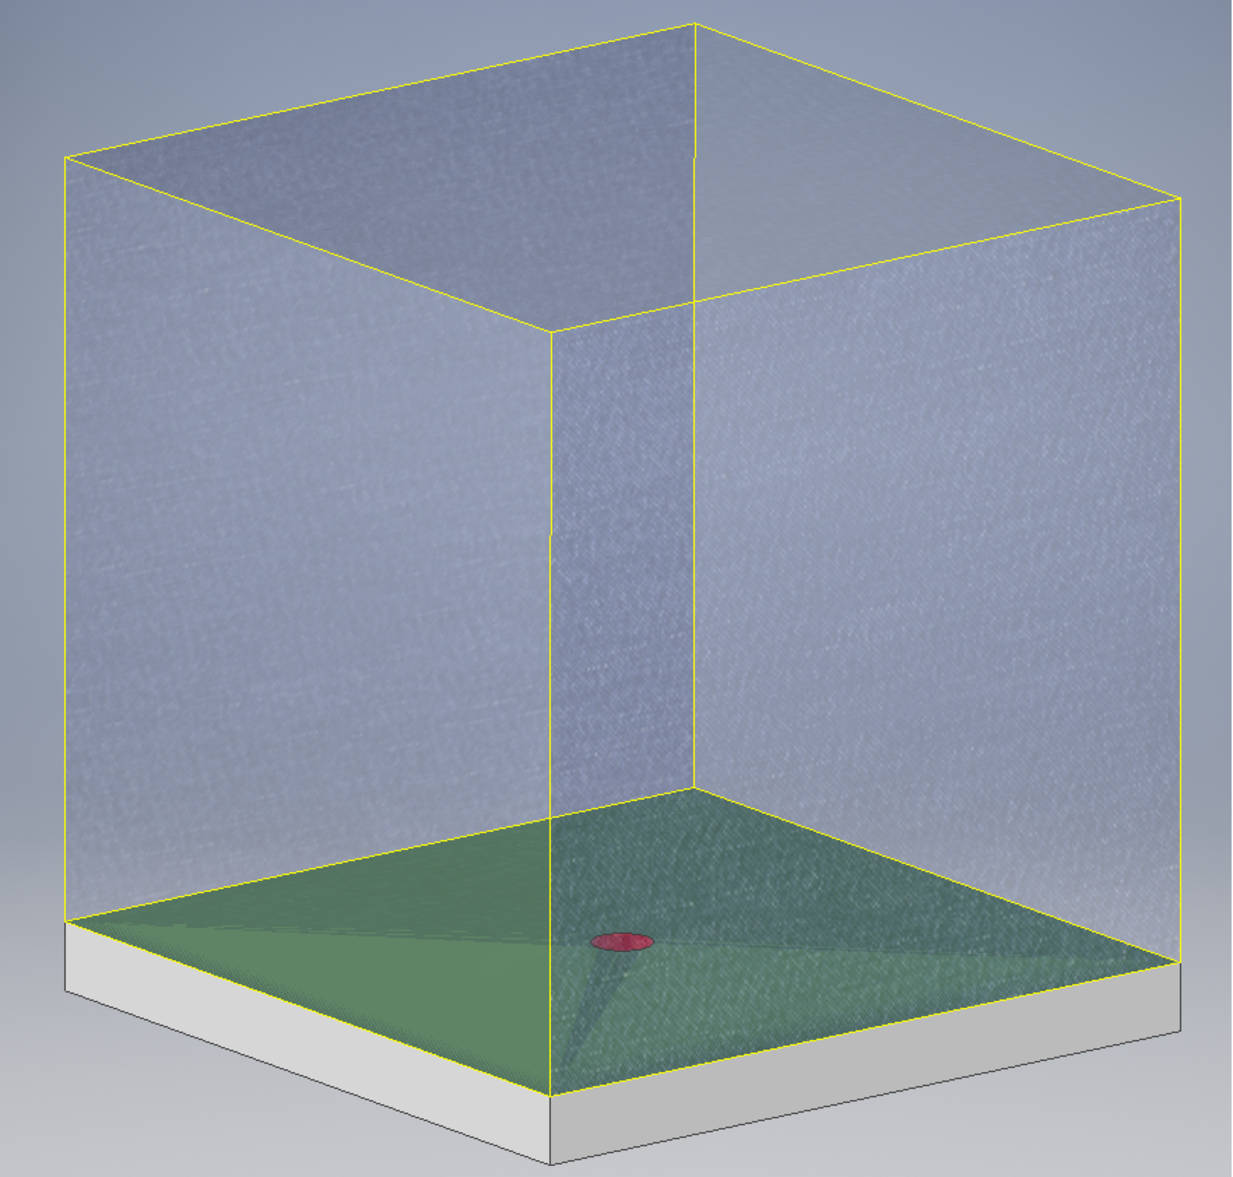
\includegraphics[width=8cm]{Chapter-2/Figures/Domain_good}
\caption{Computational domain and boundary conditions}
\label{fig:domain-BCs}
\end{figure}

\subsubsection{Velocity inlet}
At the vent, temperature of erupted material $T$, eruption velocity $\textbf{v}$, the mass fraction of vapor in erupted material $\xi_{g0}$ and mass discharge rate $\dot M$ are given. The pressure of erupted material $p$ is assumed to be the same as ambient pressure for pressure-balanced eruption. The radius of vent is determined from $\rho$, $\dot M$ and $\textbf{v}$. Equation (\ref{eq:erupt_bc_rho}) to (\ref{eq:erupt_bc_e}) gives velocity inlet boundary condition wrote in terms of primitive variables.
\begin{align}
\rho =const = p/\left(R_m T\right) \label{eq:erupt_bc_rho} \\
\xi=const=1 \label{eq:erupt_bc_xi}\\
\textbf{v} = const =\{0,0, \omega \}^T \label{eq:erupt_bc_v}\\
\dfrac{\partial e}{\partial n}=\dot M e /\left(\pi r^2\right) \label{eq:erupt_bc_e}
\end{align} 
where $r$ is the radius of the vent, $n$ is the direction normal to the boundary, value of $\omega$ can be constant or a function of location depending on the eruption profile.

\subsubsection{Non-slip wall boundary}
Velocity is zero for non-slip wall boundary. If we assume the boundary to be adiabatic, heat flux should be zero on the boundary. The flux of mass should also be zero. As a result, internal energy flux, which consists of heat flux and energy flux carried by mass flux, vanishes on the wall boundary. Equation (\ref{eq:wall_bc_rho}) to (\ref{eq:wall_bc_e}) gives no-slip wall boundary condition written in terms of primitive variables.
\begin{align}
\dfrac{\partial \rho}{\partial n} = const = 0\label{eq:wall_bc_rho} \\
\dfrac{\partial \xi}{\partial n} = const = 0 \label{eq:wall_bc_xi}\\ 
\textbf{v} = const =\{0,0,0\}^T \label{eq:wall_bc_v}\\
\dfrac{\partial e }{\partial n} = 0\label{eq:wall_bc_e}
\end{align} 

\subsubsection{Open outlet pressure boundary condition}
The pressure of the surrounding atmosphere is given. Except for the pressure, boundary values for density, velocity, and energy on the outlet should depend on the solution. As we ignore the viscosity, the shear stress is ignored and normal stress (whose magnitude equals to pressure) balances the ambient pressure.
\begin{equation}
p = p_a\left(z\right)  \label{eq:pressure_bc_p} 
\end{equation}

\section{Eigenstructure analysis}

Eigenstructures of the homogeneous governing equations is analysed to find the eigenvalues and eigenvectors, which is necessary to have better understanding on the system. In addition, it is also the basis for defining and solving of Riemann problems. In GSPH and RSPH, only a 1D Riemann problem need to be solved. So we only analyse the 1D homogeneous governing equations (Eq. (\ref{eq:gov-cs-rho-1d-hom}) $\sim$ Eq. (\ref{eq:gov-cs-e-1d-hom})) for simplification.
\begin{align}
\dfrac{\partial \rho}{\partial t} + \dfrac{\partial \rho u} {\partial x}= 0 \label{eq:gov-cs-rho-1d-hom} \\
\dfrac{\partial \rho \xi}{\partial t} + \dfrac{\partial \rho \xi u} {\partial x}= 0 \label{eq:gov-cs-ks-1d-hom}\\
\dfrac{\partial \rho u}{\partial t} + \dfrac{\partial \rho u u} {\partial x} + \dfrac{\partial p} {\partial x}= 0 \label{eq:gov-cs-v-1d-hom} \\
\dfrac{\partial \rho (e+\dfrac{1}{2}u^2)}{\partial t} + \dfrac{\partial \rho u (e+\dfrac{1}{2}u^2) } {\partial x} + \dfrac{\partial pu} {\partial x} = 0 \label{eq:gov-cs-e-1d-hom}
\end{align}
Where the vector velocity $\textbf{v}$ degenerates to a scalar velocity $u$. Equation (\ref{eq:gov-cs-rho-1d-hom}) $\sim$ (\ref{eq:gov-cs-e-1d-hom}) can be written in a more concise form:
\begin{equation}
\textbf{U(x,t)}_t + \textbf{F(\textbf{U}(x, t))}_x = 0
\end{equation}
With primitive variable vector
\begin{equation}
   \textbf{U}=\begin{bmatrix}
         u_1 \\
         u_2 \\
         u_3 \\
         u_4
     \end{bmatrix}
    =\begin{bmatrix}
         \rho \\
         \rho\xi \\
         \rho u   \\
         \rho(e+\frac{1}{2}u^2)
     \end{bmatrix}
\end{equation}
and flux vector: 
\begin{equation}
   \textbf{F}=\begin{bmatrix}
         \rho u \\
         \rho\xi u \\
         \rho u  u + p  \\
         \rho u(e+\frac{1}{2}u^2) + pu
     \end{bmatrix}
\end{equation}

It might facilitate analysis of the eigenstructure if the governing equations are formulated in terms of variables other than conserved quantities. One of the choices is using pressure in place of internal energy and using mass fraction in place of density of phase 2. Based on EOS (Eq. (\ref{eq:EOS})), the new formulation of the governing equations are obtained (see Eq. (\ref{eq:gov-PressForm-rho-1d-hom}) $\sim$ (\ref{eq:gov-PressForm-p-1d-hom}), which we refer as pressure equations in later section).

\begin{eqnarray}
\dfrac{\partial \rho}{\partial t} + u \dfrac{\partial \rho} {\partial x} + \rho \dfrac{\partial u} {\partial x}= 0 \label{eq:gov-PressForm-rho-1d-hom} \\
\dfrac{\partial \xi}{\partial t} + u \dfrac{\partial \xi} {\partial x}= 0 \label{eq:gov-PressForm-ks-1d-hom}\\
\dfrac{\partial u}{\partial t} + u \dfrac{\partial u} {\partial x} + \frac{1}{\rho} \dfrac{\partial p} {\partial x}= 0 \label{eq:gov-PressForm-v-1d-hom} \\
\dfrac{\partial p}{\partial t} + u \dfrac{\partial p} {\partial x} + \gamma_m p \dfrac{\partial u} {\partial x} = 0 \label{eq:gov-PressForm-p-1d-hom}
\end{eqnarray}
With the more concise formulation: 
\begin{equation}
\textbf{W}_t + \textbf{A(\textbf{W})} \textbf{W}_x = 0
\end{equation}
Where primitive variable vector
\begin{equation}
   \textbf{W}=\begin{bmatrix}
         w_1 \\
         w_2 \\
         w_3 \\
         w_4
     \end{bmatrix}
    =\begin{bmatrix}
         \rho \\
         \xi \\
         u   \\
         p
     \end{bmatrix}
\end{equation}
and Jacobian matrix: 
\begin{equation}
   \textbf{A(\textbf{W})}=\begin{bmatrix}
         u & 0 & \rho       & 0 \\
         0 & u & 0          & 0 \\
         0 & 0 & u          &\frac{1}{\rho} \\
         0 & 0 & \gamma_m p & u
     \end{bmatrix}
\end{equation}
The eigenvalues of the Jacobian are: $\lambda_1 = u-c$,  $\lambda_2 = \lambda_3 = u$ and $\lambda_4 = u+c$. Where $c=(\frac{\gamma_m p}{\rho})^{\frac{1}{2}}$ is the sound speed of mixture. The corresponding eigenvectors are: 
\begin{equation}
   k_1 =\begin{bmatrix}
         1 \\
         0 \\
         \frac{-c}{\rho} \\
         c^2
     \end{bmatrix},
   k_2 =\begin{bmatrix}
         1 \\
         0 \\
         0   \\
         0
     \end{bmatrix},
   k_3 =\begin{bmatrix}
         0 \\
         1 \\
         0   \\
         0
     \end{bmatrix},
   k_4 =\begin{bmatrix}
         1 \\
         0 \\
         \frac{c}{\rho} \\
         c^2
     \end{bmatrix}
     \label{eq:eigenvector-pressure}
\end{equation}

It can be proved that the characteristic fields associated with second and third eigenvalues are linear degenerate while these corresponding to first and forth are genuinely nonlinear. It is obvious that across these two waves associated with $\lambda_2$ and $\lambda_3$, only $\xi$ and $\rho$ changes, which will be proved in later section. Having an additional equation for mass fraction introduces an extra linear degenerate waves.

Based on the relationship between entropy, pressure and density (Eq. (\ref{eq:entropy-p-rho})), the governing equations can be written in term of $\rho	$, $\xi$, $u$, $s$ (the entropy).
\begin{equation}
s=C_v ln(\dfrac{p}{\rho^{\gamma_m}})+C_0 \label{eq:entropy-p-rho}
\end{equation}
Then
\begin{equation}
p=C_1 \rho^{\gamma_m} exp(\frac{s}{C_v})
\end{equation}
With $C_1=exp(-\frac{C_0}{C_v})$.
After lengthy derivation, the last governing equation can be written in terms of entropy and the complete set of governing equations (which will be referred as entropy equations in later sections) are: 
\begin{eqnarray}
\dfrac{\partial \rho}{\partial t} + u \dfrac{\partial \rho} {\partial x} + \rho \dfrac{\partial u} {\partial x}= 0 \label{eq:gov-EntropyForm-rho-1d-hom} \\
\dfrac{\partial \xi}{\partial t} + u \dfrac{\partial \xi} {\partial x}= 0 \label{eq:gov-EntropyForm-ks-1d-hom}\\
\dfrac{\partial u}{\partial t} + u \dfrac{\partial u} {\partial x} + \frac{c^2}{\rho} \dfrac{\partial \rho} {\partial x} + \frac{p ln(\rho) \Psi(\xi)}{\rho} \dfrac{\partial \xi} {\partial x} + \frac{p}{\rho C_v} \dfrac{\partial s} {\partial x} = 0 \label{eq:gov-EntropyForm-v-1d-hom} \\
\dfrac{\partial s}{\partial t} + u \dfrac{\partial s} {\partial x}= 0 \label{eq:gov-EntropyForm-e-1d-hom}
\end{eqnarray}
Where
\begin{equation}
\Psi(\xi) = \dfrac{\partial \gamma_m}{ \partial \xi}
= \frac{C_{va}R_g n_{g0} - C_{vg}R_a n_{g0} + C_{vs}R_a n_{g0} - C_{vs} R_a}{\left[(1-n_{g0}) \xi C_{vs} + \xi C_{vg} n_{g0}+(1-\xi)C_{va}\right]^2}
\end{equation}
The primitive variable vector is:
\begin{equation}
   \textbf{W}=\begin{bmatrix}
         w_1 \\
         w_2 \\
         w_3 \\
         w_4
     \end{bmatrix}
    =\begin{bmatrix}
         \rho \\
         \xi \\
         u   \\
         s
     \end{bmatrix}
\end{equation}
and the Jacobian matrix: 
\begin{equation}
   \textbf{A(\textbf{W})}=\begin{bmatrix}
         u & 0 & \rho & 0 \\
         0 & u & 0 & 0 \\
         \frac{c^2}{\rho} & \frac{ ln(\rho) \Psi(\xi) p}{\rho} & u &\frac{p}{\rho C_v} \\
         0 & 0 & 0 & u
     \end{bmatrix}
\end{equation}
The eigenvalues of the Jacobian matrix are still the same as those for pressure equations: $\lambda_1 = u-c$,  $\lambda_2 = \lambda_3 = u$ and $\lambda_4 = u+c$. While the corresponding eigenvectors are different: 
\begin{equation}
   k_1 =\begin{bmatrix}
         \frac{-\rho}{c} \\
         0 \\
         1 \\
         0
     \end{bmatrix},
   k_2 =\begin{bmatrix}
         1 \\
         0 \\
         0   \\
         -\frac{C_v c^2}{p}
     \end{bmatrix},
   k_3 =\begin{bmatrix}
         0 \\
         1 \\
         0   \\
         -C_v ln (\rho) \Psi(\xi)
     \end{bmatrix},
   k_4 =\begin{bmatrix}
         \frac{\rho}{c} \\
         0 \\
         1 \\
         0
     \end{bmatrix}
     \label{eq:eigenvector-entropy}
\end{equation}

Extra attention needed when analysing pressure equations or entropy equations as non-conservative formulations might give incorrect shock solution.
 
\section{Elementary wave solution for Riemann problem}
Based on Eigenstructure analysis in previous section, the wave structure of the system is discussed in detail in this section. 
The corresponding Riemann problem for the governing equation is defined as: 
\begin{equation}
\textbf{U(x,t)}_t + \textbf{F(\textbf{U}(x, t))}_x = 0
\end{equation}
With initial condition: 
\begin{equation}
\textbf{U}(x, 0) = \textbf{U}^0(x) = \begin{cases} 
      \textbf{U}_L & x< 0\\
      \textbf{U}_R & x\geq 0
\end{cases}
\end{equation}
As the two linear degenerate characteristic fields have the same wave speed, the solution of this Riemann Problem consists of 4 constant states separated by 4 waves (two contact discontinuities in the middle coincide). 
We assume that the initial data states $\textbf{U}_L$ and $\textbf{U}_R$ are connected by a single wave, all other waves have zero strength in the following elementary wave solution analysis.

\subsection{Contact discontinuity}
The contact discontinuity can be analysed by utilizing the Generalised Riemann Invariants. For a $m \times m$ hyperbolic system, with primitive variable $\textbf{W} = \left[ w_1, w_2, \cdot \cdot \cdot w_m \right]^T$ and right eigenvector $\textbf{K}^{(i)}=[k^{(i)}_1,k^{(i)}_2, \cdot\cdot\cdot, k^{(i)}_m]^T$. The ith Generalised Riemann Invariants are: 
\begin{equation}
\frac{dw_1}{k^{(i)}_1}=\frac{dw_2}{k^{(i)}_2}=\frac{dw_3}{k^{(i)}_3}=\cdot\cdot\cdot=\frac{dw_m}{k^{(i)}_m}
\label{eq:Generalised-Riemann-Invariants}
\end{equation}
Apply the Generalised Riemann Invariants to 2nd eigenvector of the pressure equations (Eq. (\ref{eq:gov-PressForm-rho-1d-hom}) $\sim$ (\ref{eq:gov-PressForm-p-1d-hom})): 
\begin{equation}
\frac{d \rho}{1}=\frac{d \xi}{0} = \frac{d u}{0} = \frac{d p}{0}
\end{equation}
Which implies that $xi$, $u$, $p$ keep constant across waves associated with $\lambda_2$. 
Similarly, Apply the Generalised Riemann Invariants to 3rd eigenvector of the pressure equations (Eq. (\ref{eq:gov-PressForm-rho-1d-hom}) $\sim$ (\ref{eq:gov-PressForm-p-1d-hom})):
\begin{equation}
\frac{d \rho}{0}=\frac{d \xi}{1} = \frac{d u}{0} = \frac{d p}{0}
\end{equation}
Which implies that $\rho$, $u$, $p$ keep constant across waves associated with $\lambda_3$.
To summarize $u$, $p$ keep constant across discontinuity waves associated with $\lambda_3$ and $\lambda_2$.

\subsection{Rarefaction waves}
The wave associated with $\lambda_1$ and $\lambda_4$ can be either rarefaction or shocks.
Rarefaction waves associated with genuinely nonlinear characteristic fields can also be inspected by utilizing Generalised Riemann Invariants. Apply it to $\lambda_1$ of entropy equations: 
\begin{equation}
\frac{d \rho}{-\frac{\rho}{c}}=\frac{d \xi}{0} = \frac{d u}{1} = \frac{d s}{0}
\end{equation}
So $\xi$ and $s$ keep constant. $u$ and $\rho$ have to satisfy: 
\begin{equation}
\frac{d \rho}{-\frac{\rho}{c}} = \frac{d u}{1}
\end{equation} 
Do the integral: 
\begin{equation}
u+\int \frac{c}{\rho} d\rho =const
\end{equation}
As $s$ keep constant, we can use isentropic equation: $\frac{p^{\frac{1}{\gamma_m}}}{\rho}=const$ and get: 
\begin{equation}
c^2=\gamma_m C_2 \rho^{(\gamma_m -1)}
\end{equation}
Where $C_2 = \left(\frac{p^{\frac{1}{\gamma_m}}}{\rho}\right)^{\gamma_m}$ is a constant. Plug $c$ into the integration: 
\begin{equation}
u+\frac{2c}{\gamma_m -1} = const
\label{eq:RP-solution-rarefaction-u-lamda1}
\end{equation}
Similarly, apply Generalised Riemann Invariants to $\lambda_4$ of entropy equations:
\begin{equation}
\xi = const \label{eq:RP-solution-rarefaction-xi}
\end{equation}
\begin{equation}
s = const \label{eq:RP-solution-rarefaction-s}
\end{equation}
\begin{equation}
u-\frac{2c}{\gamma_m -1} = const 
\label{eq:RP-solution-rarefaction-u-lamda4}
\end{equation}

\subsection{Shock waves}
Shock waves associated with either $\lambda_1$ or $\lambda_4$ can be analysed utilizing Rankine-Hugoniot condition. Assume a shock wave associated with $\lambda_4$ has speed $S_4$. Define the relative velocities as:
\begin{eqnarray}
\tilde{u}_L = u_L - S_4
\tilde{u}_R = u_R - S_4
\end{eqnarray}
Which transforms the frame of reference moving with the shock. Then apply Rankine-Hugoniot condition to the governing equations of conservative variables.
\begin{equation}
S=\frac{\textbf{F}(\textbf{U}_R)-\textbf{F}(\textbf{U}_L)}{\textbf{U}_R - \textbf{U}_L}
\end{equation}
As the shock keep stationary with respect to the new frame of reference:
\begin{eqnarray}
\rho_L \tilde{u}_L - \rho_R \tilde{u}_R = 0 \label{eq:RKH-rho-cs}\\
\rho_L \xi_L \tilde{u}_L - \rho_R \xi_R \tilde{u}_R = 0 \label{eq:RKH-xi-cs} \\
\rho_L \tilde{u}_L \tilde{u}_L - \rho_R \tilde{u}_R \tilde{u}_R + p_L - p_R = 0 \label{eq:RKH-u-cs} \\
(E_L + p_L) \tilde{u}_L - (E_R + p_R) \tilde{u}_R = 0 \label{eq:RKH-E-cs}\\
\end{eqnarray}
Where $E_I = \frac{1}{2} \tilde{u}^2_I \rho_I + \rho_I e_I$, with $I = L , R$.
Combining Eq. (\ref{eq:RKH-rho-cs}) and (\ref{eq:RKH-xi-cs}), we can easily conclude that $\xi_L = \xi_R$. That is to say, the mass fraction does not change across shock waves. The same conclusion can be drew for shock waves associated with $\lambda_1$ through a pretty similar analysis procedure. Recall that $\xi$ also keeps constant across rarefaction waves (Eq. (\ref{eq:RP-solution-rarefaction-xi})). Then we reach to an important conclusion: \textbf{mass fraction does not change across non-linear waves}. The eigenvectors $k_1$ and $k_4$ for pressure equations (Eq. (\ref{eq:gov-PressForm-rho-1d-hom}) $\sim$ (\ref{eq:gov-PressForm-p-1d-hom})) also implies that $\xi$ does not change across any non-linear waves (either shock or rarefaction).

\section{Decouple of mass fraction equation from other governing equations}
\begin{figure}
\center
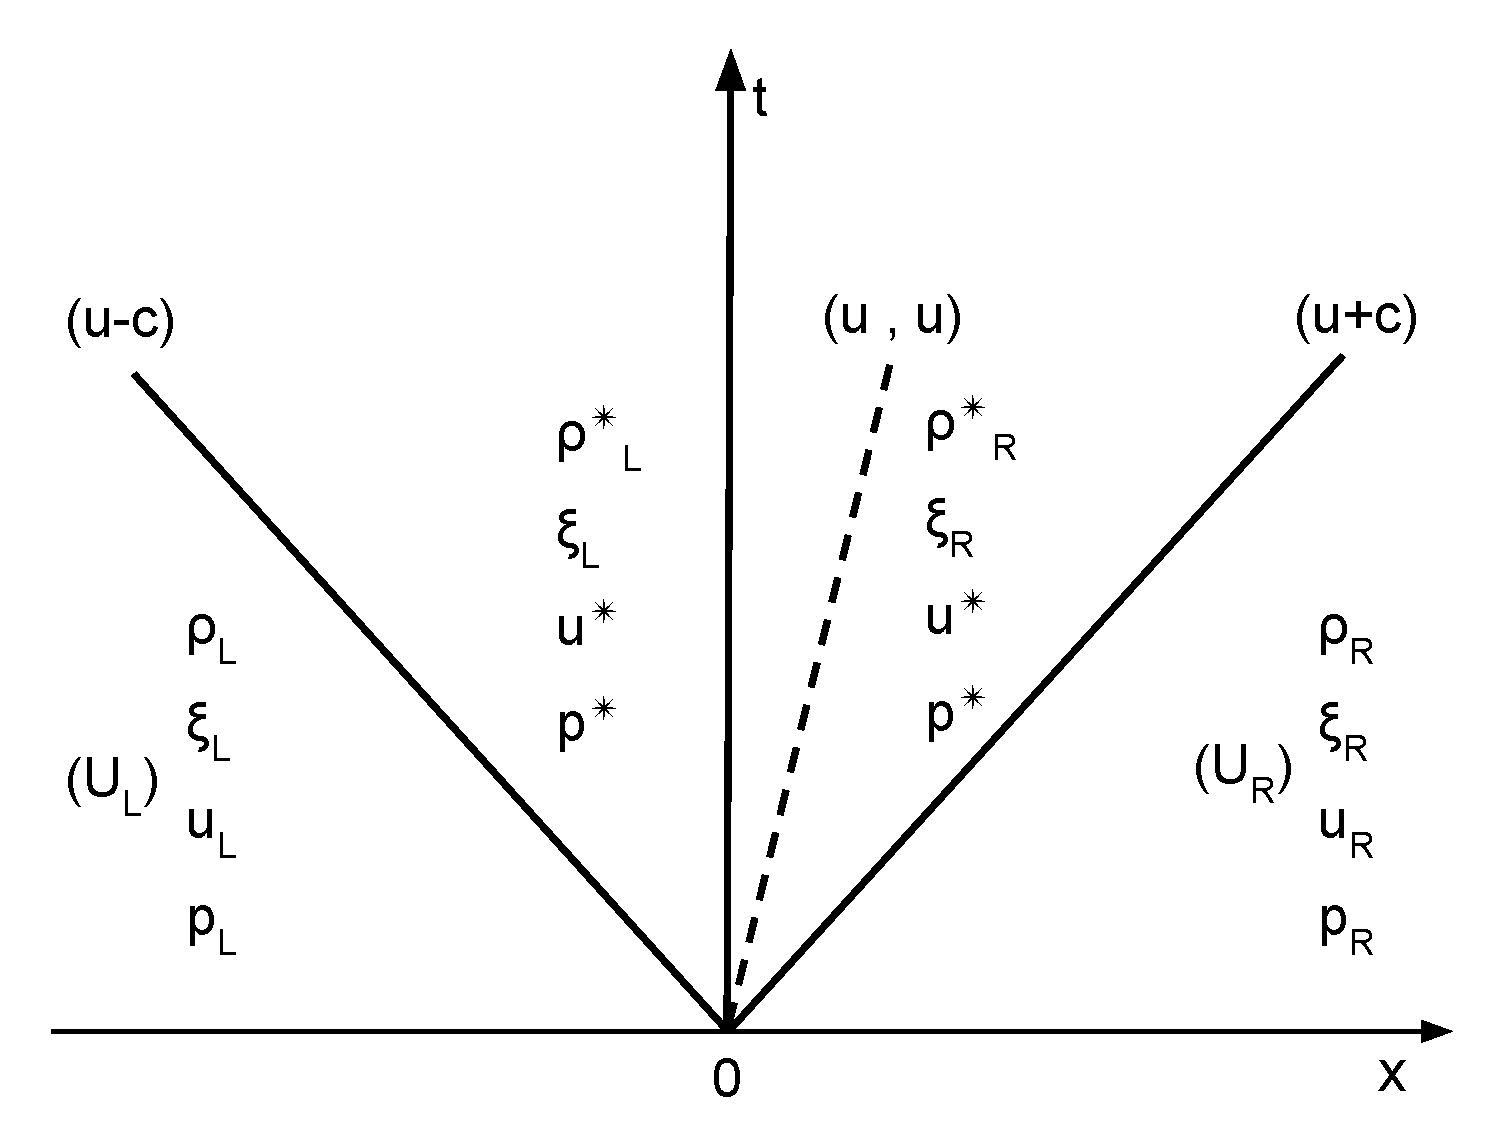
\includegraphics[width=6cm]{Chapter-2/Figures/Solution_Structure_RP}
\caption{The solution structure of Riemann problem for Plume-SPH governing equations}
\label{fig:Solution_Structure_RP}
\end{figure}
Based on the analysis on elementary wave solution for single waves, we get the structure of the solution of Riemann problem for system of governing equations as shown in Fig \ref{fig:Solution_Structure_RP}. The solution of mass fraction $\xi$ can be obtained separately from solving of other equations.
\begin{equation}
\xi =  \begin{cases} 
      \xi_L & x< ut\\
      \xi_R & x > ut
\end{cases}
\label{eq:RP_solution_xi}
\end{equation}
Since the solution of $\xi$ is independent of types of non-linear waves propagating left and right. $\xi$ can be updated separately before solving Riemann problems. This is easy to implement in discretized governing equations. The same discretized formulations (Eq. (\ref{eq:gov-sph-xi})) can be used to update mass fraction in GSPH.
\begin{figure}
\center
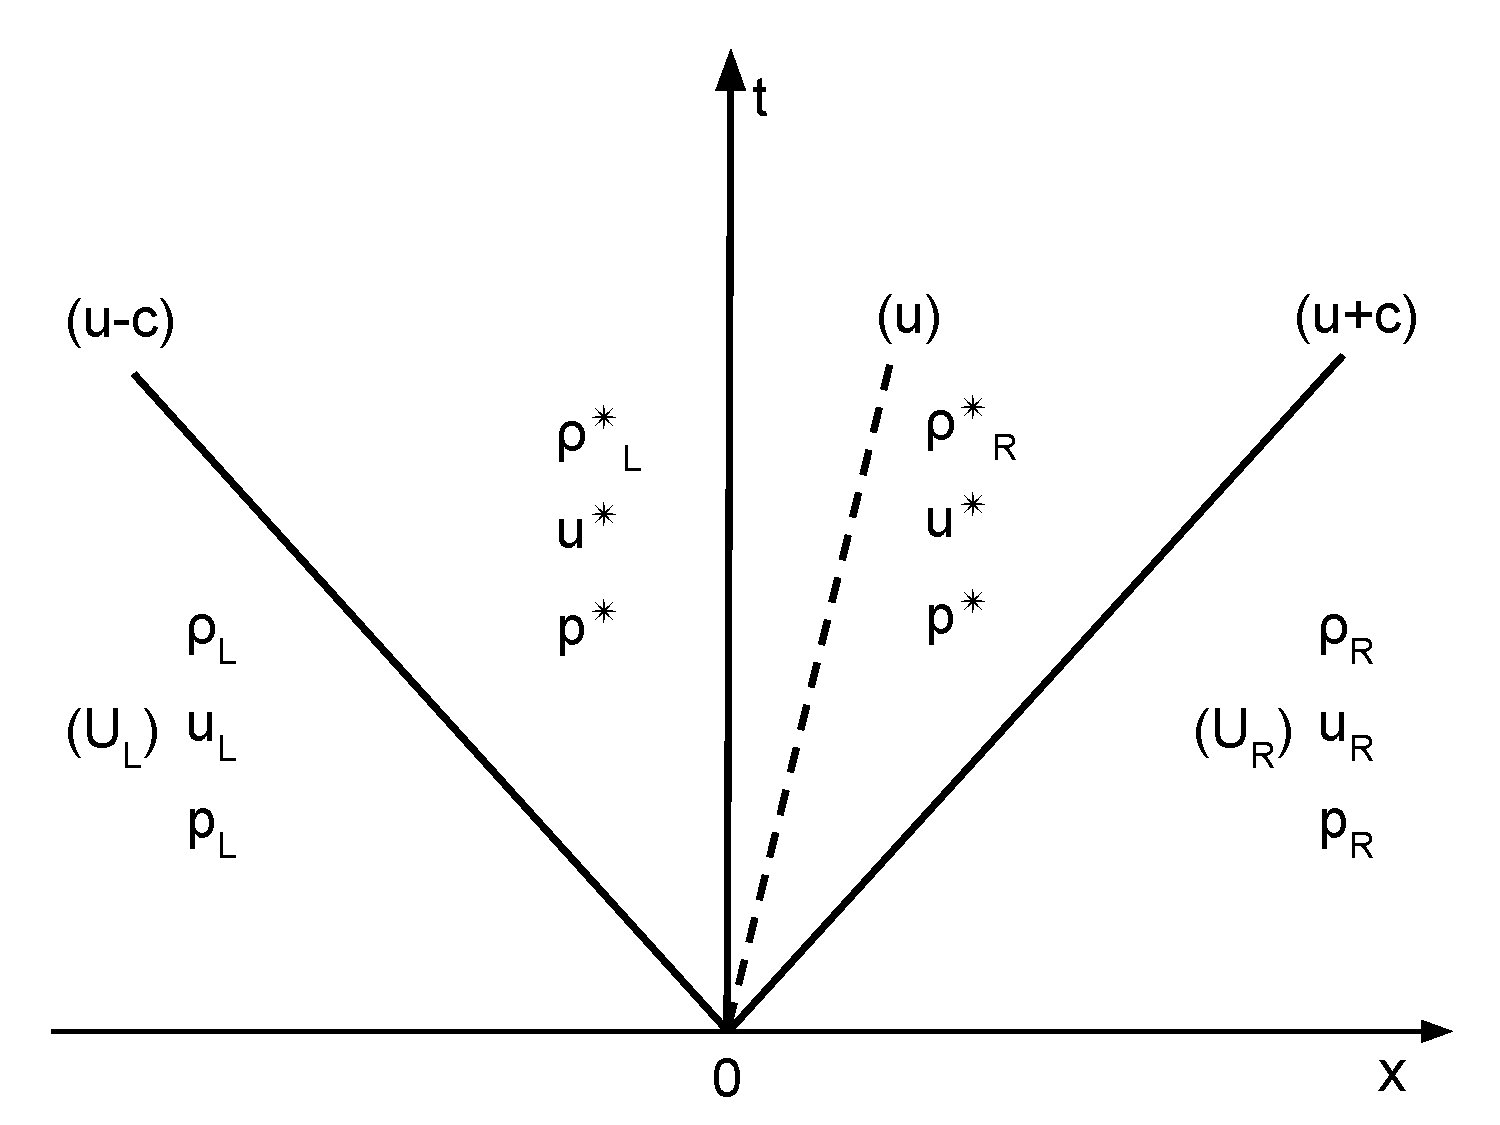
\includegraphics[width=6cm]{Chapter-2/Figures/Solution_Structure_RP_simplified}
\caption{The simplified solution structure of Riemann problems for Plume-SPH governing equations. The simplified solution structure is the same as that for Euler equation.}
\label{fig:Solution_Structure_RP_simplified}
\end{figure}
As the second equation in the original governing equations (Eq. (\ref{eq:gov-cs-rho}) $\sim$ (\ref{eq:gov-cs-e})) are weakly coupled with others and can be solved separately within each time step. Then remove Eq. (\ref{eq:gov-cs-ks}) from the original governing equations, the left will become Euler Equations. Equation (\ref{eq:gov-cs-rho}), (\ref{eq:gov-cs-v}), (\ref{eq:gov-cs-e}) together with Eq. (\ref{eq:EOS}) will form a complete system of equations with a space and time dependent $\gamma_{m}$. The solution structure of Riemann problems can be simplified as shown in Fig. \ref{fig:Solution_Structure_RP_simplified}, which is exactly the same as solution structure for Euler equations. There are plenty of (exact and approximate) Riemann solvers for Euler equations ready to use. Equation (\ref{eq:gov-nc-ks}) together with other equations, Eq. (\ref{eq:gov-gm}) - Eq. (\ref{eq:gov-ns}) will only be used to updating $\gamma_{m}$ which is a function of $\xi$. It is a separate procedure to update $\xi$ in SPH. Based on above analysis, it can be also a separate one in GSPH. In this way, equations are divided into two relatively independent groups, one represents Euler equations and the other one for updating $\gamma_{m}$.
The GSPH formulism \citep{inutsuka2002reformulation} proposed for solving Euler equations can be directly used. In this case, we can use usual Riemann solvers for ideal gas (with a time and space dependent $\gamma$). Input variables for Riemann solvers will be $\rho=\rho^a + \rho^{sg}$, prssure $p$ and velocity $\textbf{v}$.
 
The only trick is, in this case, the specific heat ratio $\gamma_{m}$ is not a constant in space and time. Usually exact Riemann solvers for ideal gas are developed based on constant $\gamma_{m}$ assumptions. And exact Riemann solver for not-constant gamma need to be driven in that case. Some numerical trick can be used. For example, when calculate $p^{ast}$ for the pair of two particles $\alpha$ and $\beta$, We can use Riemann solvers for a constant $\gamma_{m}=\frac{\gamma_{m,\alpha}+\gamma_{m,\beta}}{2}$.
Numerically, this treatment is sufficient. 

\chapter{Classical SPH Method} \label{chapter:classical-SPH}

\section{Introduction}
A mesh-free Lagragian method, SPH, is selected to numerically solve governing equations. There are several review papers by \citet{monaghan1992smoothed, monaghan2005smoothed, rosswog2009astrophysical, price2012smoothed, monaghan2012smoothed}, giving a pretty comprehensive view over SPH. We only refer here to the representation of the constitutive equations in SPH and put more focus on specific numerical techniques for plume modeling.

In SPH, the domain is discretized by a set of particles or discretization points and the position of each particle is updated at every time step based on the motion computed. Approximation of all field variables (velocity, density and pressure, ect.) is obtained by interpolation based on discretization points. The physical laws (such as conservation laws of mass, momentum and energy) written in the form of PDEs (partial differential equations) or ODEs (ordinary differential equations) need to be transformed into the Lagrangian particle formalism of SPH. Using a kernel function that provides the weighted estimation of the field variables at any point, the integral equations are estimated as sums over particles in a compact subdomain defined by the support of the kernel function associated with the discretization points. Thus, field variables associated to the particle are updated based on its neighbors. Each kernel function has a compact support determined by smoothing length of each particle.

\section{Fundamental principles}
There are several procedures for discretizing governing equations (PDEs or ODEs) with SPH. We present here one of them following \citet{monaghan1992smoothed, monaghan2005smoothed, monaghan2012smoothed}. The starting point of approximating a function with SPH is the translation property of the Dirac function $\delta(\textbf{x})$, for an arbitary function $A(\textbf{x})$, the following equation holds. 
\begin{equation}
A\left(\textbf{x}\right)=\int_{-\infty}^{\infty} A\left(\textbf{x} \prime\right) \delta \left(\textbf{x} \prime - \textbf{x}\right) d\textbf{x} \prime
\label{eq:Dirac-translation}
\end{equation}
The Dirac function in Eq. (\ref{eq:Dirac-translation}) can be approximated by a weighting function $w\left(\textbf{x}-\textbf{x}\prime, h\right)$ (or $w\left(\textbf{x}\prime-\textbf{x}, h\right)$) which tends to a Dirac function when the smoothing length $h \rightarrow 0$ :
\begin{equation}
\lim _{h \rightarrow 0} w\left(\textbf{x} \prime-\textbf{x}, h\right) =  \delta \left(\textbf{x} \prime - \textbf{x}\right)
\label{eq:SPH_kernel_delta}
\end{equation}
So it can be viewed as an approximate form of the Dirac function and should satisfy the normalization condition:
\begin{equation}
\int	 w\left(\textbf{x}-\textbf{x}\prime, h\right) d\textbf{x}\prime = 1
\label{eq:SPH-kernel-normalization-prop}
\end{equation}
Besides normalization, the weighting function of particle $a$ has to be symmetric with respect to $a$ to ensure that neighbor particles located at the same distance away from $a$ contribute equally to SPH summation equation, see Eq. (\ref{eq:SPH-kernel-symmetric}).
\begin{equation}
w\left(\textbf{x}- \textbf{x} \prime, h\right) = w\left(\textbf{x} \prime - \textbf{x}, h\right)
\label{eq:SPH-kernel-symmetric}
\end{equation}
The weighting function also needs to satisfy conditions such as positivity and compact support. In addition, the kernel function must be monotonically decreasing with the distance between particles.

There is a wide variety of possible weighting functions that can satisfy these requirements, such as spline functions (with different orders) and Gaussian functions. Generally, the accuracy increases with the order of the polynomials of the kernel function, but the computational cost also increases as number of interactions increase. 
We are adopting a truncated Gaussian function as the weighting function in our simulation.
\begin{equation}
w\left(\textbf{x} - \textbf{x} \prime \right) = 
\begin{cases} 
      \dfrac{1}{\left(h \sqrt{\pi}\right)^d} exp \left[- \left(\dfrac{\textbf{x} - \textbf{x} \prime}{h} \right)^2 \right] &  \vert \textbf{x} - \textbf{x} \prime \vert \leq 3h\\
      0 & \text{Otherwise}
\end{cases}
\label{eq:SPH-kernel}
\end{equation}
where $d$ is number of dimensions.
The derivative of the weighting function is:
\begin{equation}
\nabla w\left(\textbf{x} - \textbf{x} \prime \right) = 
\begin{cases} 
      -2\left(\dfrac{\textbf{x} - \textbf{x} \prime}{h}\right) \dfrac{1}{\left(h \sqrt{\pi}\right)^d} exp \left[- \left(\dfrac{\textbf{x} - \textbf{x} \prime}{h}\right)^2 \right] &  \vert \textbf{x} - \textbf{x} \prime \vert \leq 3h\\
      0 & \text{Otherwise}
\end{cases}
\label{eq:SPH-kernel-gradient}
\end{equation}

By replacing $\delta$ function in Eq. (\ref{eq:SPH_kernel_delta}) with the kernel function $w$, an arbitrary function $A\left(\textbf{x}\right)$ can then be approximated by:
\begin{equation}
A\left(\textbf{x}\right) \approx <A\left(\textbf{x}\right)> = \int_{\Omega} A\left(\textbf{x} \prime\right) w\left(\textbf{x}-\textbf{x}\prime, h\right) d\textbf{x}\prime + O\left(h^2\right)
\label{eq:SPH-fundamental-principle}
\end{equation}
As the weighting function is symmetric (Eq. (\ref{eq:SPH-kernel-symmetric})) and satisfies the normalization condition (Eq. (\ref{eq:SPH-kernel-normalization-prop})), odd error terms in Eq. (\ref{eq:SPH-fundamental-principle}) vanishe leading to a second order approximation. However, in practice, second order of accuracy can not be achieved because there is no guarantee on the symmetry of particle distribution in real simulation \citep{price2012smoothed}.
Recall that $d\textbf{x}\prime = \dfrac{dm (\textbf{x} \prime)}{\rho (\textbf{x} \prime)}$, the integration equation, Eq. (\ref{eq:SPH-fundamental-principle}), can be approximated by summation and lead to an approximation of the function $A$:
\begin{equation}
<A\left(\textbf{x}\right)> \approx \sum_b m_b \dfrac{A_b}{\rho_b} w\left(\textbf{x}-\textbf{x}_b, h\right)
\label{eq:SPH-approximation-sum}
\end{equation}
where the summation is over all the particles within the region of compact support (See Eq. (\ref{eq:SPH-kernel})) of the weighting function. 
Gradient terms may be straightforwardly calculated by taking the derivative of Eq. (\ref{eq:SPH-approximation-sum}), giving
\begin{equation}
\begin{split}
<\nabla A\left(\textbf{x}\right)> & = \dfrac{\partial }{\partial \textbf{x}} \int_{\Omega} A\left(\textbf{x} \prime\right) w\left(\textbf{x}-\textbf{x}\prime, h\right) d\textbf{x}\prime + O\left(h^2\right) \\
& \approx \sum_b m_b \dfrac{A_b}{\rho_b} \nabla w\left(\textbf{x} - \textbf{x}_b, h\right)
\end{split} 
\label{eq:SPH-scalar-function-gradient}
\end{equation}
For vector quantities the expressions are similar, simply replacing $A$ with $\textbf{A}$ in Eq. (\ref{eq:SPH-approximation-sum}) and Eq. (\ref{eq:SPH-scalar-function-gradient}), giving
\begin{align}
<\textbf{A}\left(\textbf{x}\right)> \approx \sum_b m_b \dfrac{\textbf{A}_b}{\rho_b} w\left(\textbf{x}-\textbf{x}_b, h\right) \\
<\nabla \cdot \textbf{A}\left(\textbf{x}\right)> \approx \sum_b m_b \dfrac{\textbf{A}_b}{\rho_b} \cdot \nabla w\left(\textbf{x} - \textbf{x}_b, h\right) \\
<\nabla \times \textbf{A}\left(\textbf{x}\right)> \approx \sum_b m_b \dfrac{\textbf{A}_b}{\rho_b} \times \nabla w\left(\textbf{x} - \textbf{x}_b, h\right) \\
<\nabla^j \textbf{A}^i\left(\textbf{x}\right)> \approx \sum_b m_b \dfrac{\textbf{A}_b^i}{\rho_b} \nabla^j w\left(\textbf{x} - \textbf{x}_b, h\right) 
\label{eq:SPH-vecctor-function}
\end{align}

\section{Adaptive smoothing length}
The spatial resolution of SPH is determined by the smoothing length, $h$. It is common for each particle to have its own time dependent smoothing length which adapts according to the local number density of particles. Adaptive smoothing length can automatically match the resolution length $h$ to the scale of the system and is especially necessary in certain scenarios where density varies in a large range, for example, Sj$\ddot{o}$green tests.
The adaptivity of smoothing length is less important for incompressible flow while pretty necessary for compressible flow. There are two different ways adjust the smoothing length.

One robust way of specifying the smoothing length $h$ is proposed by \citet{gingold1978binary}. He suggested that changing of the smoothing length should be related to density according to: 
\begin{equation}
h_a = \sigma \left(\frac{m_a}{\rho_a}\right)^{\frac{1}{d}}
\label{eq:adptive-sml-Gingold}
\end{equation}
Where $d$ is number of dimensions and he suggested to use 1.3 for $\sigma$.
There are many varitions of this formulation. For example, \citet{steinmetz1993capabilities} suggested to use averaged local density to determine the smoothing length. \citet{hernquist1989treesph} suggested to keep number of neighbour particles constatnt by adjusting smoothing length. \citet{inutsuka2002reformulation} suggested to use a more smooth density to avoid large varying of smoothing length within the neighborhood of each particle.
Equation (\ref{eq:adptive-sml-Gingold}) is a nonlinear equation for the single variable $\rho_a$  which can be solved rapidly by point iteration possibly combined with a Newton-Raphson scheme.

The introduction of time varying smoothing lengths can, however, lead to serious problems with and momentum energy conservation in certain situations \citep{hernquist1993some}. Few attention has been paid to losing of strict conservation feature in original SPH discretization when smoothing length varies in time and space. The problem arises from the fact that the use of variable smoothing lengths means that additional terms \citep{nelson1994variable} should appear in the particle equations of motion. In our implementation, we adopt a simple strategy \citep{evrard1988beyond}: $h$ takes the average of $h_a$ and $h_b$. Such strategy can help restore the strict conservation feature of classical SPH discretization providing that the two paired particles are in ``pool of neighbouring particles" of each other. 

\section{Artificial viscosity} \label{sec:artificial-viscosity}
In classical SPH, shock waves are handled by introducing artificial viscosity, a term that is defined based on second derivatives of velocity, to smear out discontinuities. As in the case of first order derivatives, second order derivatives can be estimated by differentiating a SPH interpolation twice. However, such a formulation has two disadvantages: first, it is very sensitive to irregular distribution of particles, second, the second derivative of the kernel can change sign and lead to unphysical representations (for example, viscous dissipation causes decrease of the entropy). 

One of the most commonly used models of artificial viscosity \citep{monaghan1983shock} is:
\begin{equation}
\Pi_{ab}=- \frac{\nu}{\bar{\rho}_{ab}} \dfrac{ \textbf{v}_{ab} \cdot \textbf{x}_{ab}}{\textbf{x}_{ab}^2 + \left(\eta h\right)^2}
\label{eq:art-vis-original}
\end{equation}
The coefficient $\nu$ is defined as:
\begin{equation}
\nu = \alpha \bar{h}_{ab} \bar{c}_{ab}
\end{equation}
where 
\begin{align}
\bar{c}_{ab} = \dfrac{c_a + c_b}{2} \\
\bar{\rho}_{ab} = \dfrac{\rho_a + \rho_b}{2} \\
\textbf{v}_{ab}=\textbf{v}_a-\textbf{v}_b \\
\textbf{x}_{ab}=\textbf{x}_a-\textbf{x}_b
\end{align}
The artificial viscosity term $\Pi_{ab}$ is a Galilean invariant and vanishes for rigid rotation. It produces a repulsive force between two particles when they are approaching each other and an attractive force when they are receding from each other. 

The SPH viscosity can be related to a continuum viscosity by converting the summation to integrals \citep{monaghan2005smoothed}. It has been shown that  shear viscosity coefficient $\eta = \frac{\rho \alpha h c}{8} $ and bulk viscosity coefficient $ \zeta = \frac{5 \eta}{3}$ are appropriate for two dimensional flows and modified to $\eta = \frac{\rho \alpha h c}{10} $ , $ \zeta = \frac{5 \eta}{3}$ for three dimensional flows.
An extra term was added to $\nu$ considering aspects of the dissipative term in shock solutions based on Riemann solvers and lead to a new formulation of artificial viscosity. We adopt this new formulation in our simulation:
\begin{equation}
\Pi_{ab}^{\beta} = 
\begin{cases} 
      \dfrac{- \alpha \mu_{ab} \bar{c}_{ab} + \beta \mu_{ab}^2} {\bar{\rho}_{ab}} & \textbf{v}_{ab} \cdot \textbf{x}_{ab} < 0\\
      0 & \textbf{v}_{ab} \cdot \textbf{x}_{ab} > 0
\end{cases}
\label{eq:art-vis-shock}
\end{equation}
where
\begin{equation}
\mu_{ab} = \dfrac{h \textbf{v}_{ab} \cdot \textbf{x}_{ab}}{\textbf{x}_{ab}^2 + \left(\eta h\right)^2} 
\end{equation}
%$\alpha$ and $\beta$ are two parameters that are free to be adjusted for each case. 
$\alpha$ and $\beta$ are two parameters that can be adjusted for different cases.
$\alpha = 1$ and $\beta = 2$ are  recommended by Monaghan for best results. In our simulation, these two parameters are calibrated to  $\alpha = 0.3$ and $\beta = 0.6$. $\eta$ is usually taken as 0.1 to prevent singularities.
%when $\textbf{x}_{ab} = 0$.

\section{Discretization of Euler equations and extensibility}
The basic interpolation given in Eq. (\ref{eq:SPH-approximation-sum}) to Eq. (\ref{eq:SPH-vecctor-function}) provides a general way to obtain SPH expressions of governing equations. The problem is that using these expressions ``{as is}" in general leads to quite poor gradient estimates. Various tricks can be used to conserve linear and angular momentum and thermal energy \citep{monaghan1992smoothed}. Special treatments are also needed for second order derivative terms \citep{monaghan2005smoothed}. We only refer here to one of these possible discretizations of compressible Euler equations with SPH:
\begin{align}
<\rho_a> = \sum_b m_b w_{ab} \left(h\right) \label{eq:ns-sph-d} \\
\left\langle\dfrac{d \textbf{v}_a}{d t}\right\rangle = -\sum_b m_b \left(\dfrac{p_b}{\rho_b^2} + \dfrac{p_a}{\rho_a^2} + \Pi_{ab}\right) \nabla_a w_{a b}\left(h\right) +\textbf{g} \label{eq:ns-sph-v} \\
\left\langle\dfrac{d e_a}{d t}\right\rangle=
 0.5\sum_b m_b \textbf{v}_{a b}\left(\dfrac{p_b}{\rho_b^2} + \dfrac{p_a}{\rho_a^2} + \Pi_{ab}\right) \cdot \nabla_a w_{a b}\left(h\right) \label{eq:ns-sph-e}
\end{align}
where, $a$ is the SPH particle index, $\textbf{v}_{a b} = \textbf{v}_a - \textbf{v}_b$. $\Pi$ is an artificial viscosity term, which is discussed in section \ref{sec:artificial-viscosity}. $w_{a b}\left(h\right)$ is a concise form of $w\left(\textbf{x}_a - \textbf{x}_b, h\right)$ and from here on, we will use this concise form.
%However, these discretized formulations will not guarantee conservation of entropy. We can obtain conservation of entropy by giving up on conservation of mass or thermal energy adopting  alternative discretized formulations \citep{monaghan1992smoothed}.
As a Lagrangian method, particle position is also updated at every time step.
\begin{equation}
\left\langle\dfrac{d \textbf{x}_a}{dt}\right\rangle = \textbf{v}_a \label{eq:SPH-update-pos}
\end{equation}

We highlight an important feature of the SPH methodology. Adding new physics and new phases into the model is trivial in terms of discretization. For example, adding of new source (or sink) into Eq. (\ref{eq:ns-sph-d}), adding a drag force into Eq. (\ref{eq:ns-sph-v})  and adding a heat exchange term into Eq. (\ref{eq:ns-sph-e}) leads to the new discretization form:
\begin{align}
<\rho_a> = \sum m_b w_{ab} \left(h\right) + \dot{\rho}\left(\textbf{x},t\right)\label{eq:ns-source-sph-d} \\
\left\langle\dfrac{d \textbf{v}_a}{d t}\right\rangle= -\sum_b m_b \left(\dfrac{p_b}{\rho_b^2} + \dfrac{p_a}{\rho_a^2} + \Pi_{ab}\right) \nabla_a w_{a b}\left(h\right) +\textbf{g} + D \sum	_b m_b \dfrac{\textbf{v}_b - \textbf{v}_a}{\rho_b} \label{eq:ns-drag-sph-v}
\end{align}
\begin{equation}
\begin{split}
\left\langle\dfrac{d e_a}{d t}\right\rangle
&= 0.5\sum_b m_b \textbf{v}_{a b}\left(\dfrac{p_b}{\rho_b^2} + \dfrac{p_a}{\rho_a^2} + \Pi_{ab}\right) \cdot \nabla_a w_{a b}\left(h\right) \\
&+ \sum_b \dfrac{m_b}{\rho_b}\left(\kappa_a + \kappa_b\right) \dfrac{\left(T_a - T_b\right)}{\textbf{r}_a - \textbf{r}_b} w_{ab}\left(h\right) \label{eq:ns-conduction-sph-e}
\end{split}
\end{equation}

where the source term $\dot{\rho}$ can be a "sink" of erupted vapor due to its phase change.
%(see microphysics modelling in ATHAM \citep{oberhuber1998volcanic}).
$D$ is a drag force coefficient. $\kappa$ is the heat conduction coefficient. $T$ is the temperature. Other physics can be added easily in a similar way. Adding of these new terms leads to modification of only a few lines in the source code. The drag force term should show up when dynamic disequilibrium between different phases is considered. In that case, each phase needs one set of governing equations of Navier-Stokes type. Adding of new phase into SPH code only needs adding few new lines for the new phase besides interaction terms introduced by the new phase.

\section{Time step}
The physical quantities (velocity, density and pressure) and particle position change every time step. The Courant condition, which is in spirit similar to the Courant condition for the mesh-based methods, is used to determine the time step $\Delta t$.
\begin{equation}
\Delta t = \textrm{CFL} \min_a \bigg \lbrace \dfrac{\left[\frac{m_a}{\rho_a}\right]^{\frac{1}{d}}}{c_a} \bigg \rbrace
\end{equation}
where $c_a$ is sound speed at particle $a$ and calculated based on heat specific ration of the mixture $\gamma_m$ (See Eq. (\ref{eq:sound-speed-mixture})). 
$d$ is number of dimensions. 
\begin{equation}
c_a = \left( \gamma_m \frac{p}{\rho} \right)^{0.5}
\label{eq:sound-speed-mixture}
\end{equation}

First order Euler integration, with $\textrm{CFL} = 0.2$, is used to advance in time.

\section{Tensile instability and corrected derivatives}
The classical SPH method was known to suffer from tensile instability and boundary deficiency. Tests of the standard SPH method indicate an instability in the tensile regime, while the calculations are stable in compression.  A simple example of such a test calculation exhibiting the instability involves a body which is subjected to an uniform initial stress, either compressive or tensile. If the initial stress is tensile, a very small velocity perturbation on a single particle can lead to particles clumping together, forming large voids and seriously corrupting density distribution. But if the initial stress is compressive, the small velocity perturbation on a single particle can not lead to any changes in particle distribution \citep{swegle1995smoothed}. To address these difficulties, \citep{chen1999improvement} proposed a corrected SPH formulation. For 1D case, employing a Taylor expansion for $A\left(x\right)$ about $x_a$, multiplying both sides by kernel function and then doing integration over the domain gives
\begin{equation}
\begin{split}
\int_{\Omega} A\left(x\right) w\left(x- x_a, h\right) dx 
& = A_a \int_{\Omega} w\left(x - x_a, h\right) dx \\
&+\dfrac{\partial A}{\partial x}(x_a) \int_{\Omega} \left(x-x_a\right) w\left(x - x_a, h\right) dx +...
\end{split}
\end{equation}
Ignoring derivative terms higher than first order, and writing the integral in particle approximation form leads to:
\begin{equation}
A_a = \frac{\sum_b m_b \dfrac{A_b}{\rho_b} w\left(x_a-x_b, h\right)}{\sum_b m_b \dfrac{1}{\rho_b} w\left(x_a-x_b, h\right)}
\label{eq:CSP-function-approximation-1d}
\end{equation}
Notice that the denominator in Eq. (\ref{eq:CSP-function-approximation-1d}) is actually summation approximation of Eq. (\ref{eq:SPH-kernel-normalization-prop}). That is to say, Eq. (\ref{eq:CSP-function-approximation-1d}) and Eq. (\ref{eq:SPH-approximation-sum}) are the same for particles far away from boundaries as the denominator in Eq. (\ref{eq:CSP-function-approximation-1d}) becomes $1$ in that case.
The first order derivative term can be obtained in a similar way:
\begin{equation}
\nabla A_a = \frac{\sum_b m_b \dfrac{A_b - A_a}{\rho_b} \nabla_a w\left(x_a-x_b, h\right)}{\sum_b m_b \dfrac{x_b - x_a}{\rho_b} \nabla_a w\left(x_a-x_b, h\right)}
\end{equation}

For problems of higher dimension, the expressions for function approximation are exactly the same as Eq. (\ref{eq:CSP-function-approximation-1d}), even though the derivation is different. The first order derivative can be obtained by solving system of equations explicitly or numerically \citep{chen1999improvement}.

\section{Mass fraction update}
Air and erupted material are represented by two different sets of SPH particles (or discretization points) in the model. Based on assumptions we made in section \ref{sec:chp2-Mathematical-Description}, only density needs to be updated respectively for each phase. Such assumption also eliminate the tension forces accross the interface and simplified numerical challenges. The updating of density is exactly the same as Eq. (\ref{eq:ns-sph-d}) in spirit.  Particles of phase 1 are not be counted while evaluating density of phase 2 and vice versa. Updating of density is then based on the following discretized equations.
\begin{equation}
<\rho_{\alpha}^a>=\frac{\sum m_b w_{\alpha b} \left(h\right)}{\sum \frac{m_b}{\rho_b} w_{\alpha b} \left(h\right) +\sum \frac{m_j}{\rho_j} w_{\alpha j} \left(h\right)} \label{eq:gov-sph-d1}
\end{equation}
\begin{equation}
<\rho_\alpha^{sg}>=\frac{\sum_j m_j w_{\alpha j} \left(h\right)}{\sum \frac{m_b}{\rho_b} w_{\alpha b} \left(h\right) +\sum \frac{m_j}{\rho_j} w_{\alpha j} \left(h\right)} \label{eq:gov-sph-d2}
\end{equation}
where the subscript $a$ and $b$ represents air particles (phase 1) while $i$ and $j$ represents erupted material. $\beta$ and $\alpha$ represents either erupted material or air.
$\rho_a^a$ is density of phase 1 (air). 
 $\rho_i^{sg}$ is density of phase 2 (erupted material).
$\rho=\rho^a + \rho^{sg}$ is density of mixture of air and erupted material. 
By definition, the mass fraction is updated according to Eq. (\ref{eq:gov-sph-xi}).
\begin{equation}
<\xi_{\alpha}> = \dfrac{\rho^{sg}_{\alpha}}{\rho_{\alpha}}
\label{eq:gov-sph-xi}
\end{equation}

In areas far away from the interface, updating of density is exactly the same as that for single phase flow. For example, in the right side and left side (or blue areas) in Fig. \ref{fig:SPH-multiple-density}, where there are only air particles, Eq.  (\ref{eq:gov-sph-d2}) evaluates to zero and total density is:
\begin{equation}
\rho_{\alpha}=\rho_{\alpha}^a=\frac{\sum m_b w_{\alpha b} \left(h\right)}{\sum \frac{m_b}{\rho_b} w_{\alpha b}}
\end{equation}
Which is a special case of Eq. (\ref{eq:CSP-function-approximation-1d}). For these areas occupied by only particles of phase 2 and far away from the interface, similarly, the equation for density update becomes: 
\begin{equation}
\rho_{\alpha}=\rho_{\alpha}^{sg}=\frac{\sum m_j w_{\alpha j} \left(h\right)}{\sum \frac{m_j}{\rho_j} w_{\alpha j}}
\end{equation}
That is to say, the same density updating equation can be applied for both phases and no additional numerical treatment needed to locate where the interface is.

\begin{figure}
\center
\includegraphics[width=12cm]{Chapter-3/Figures/Interface}
\caption{In the left figure, the blue particles (phaseID=1) represent air particles the red ones (phaseID=2) represent erupted material. The right figure shows corresponding mass fraction. Mass fraction are evaluated based on Eq. (\ref{eq:gov-sph-d1}) and Eq. (\ref{eq:gov-sph-d1}) without any other interface track or capture method.}
\label{fig:SPH-multiple-density}
\end{figure}

Interface construction will become necessary and important when attempt to include the effects of mixing by resolving the detailed interface structure and dynamics of turbulence. 
As a Lagrangian method, interface tracking in SPH is explicit through capturing of the locations of the particles, much simplier than Euleruan Methods.
The existence of complex evolving interfaces between phases presents severe challenges to conventional Eulerian grid-based numerical methods. Either interface tracking (Lagrangian) \citep{harlow1965numerical, wrobel1991computational, cheng1995simplified} or interface capturing (Eulerian) \citep{hirt1981volume, youngs1982time, gerlach2006comparison, gopala2008volume} methods are used to reconstruct the flow interface of free boundary flow. High computational cost, a tendency to form numerical instabilities and the inability to track complex topological changes are the significant drawbacks of tracking techniques \citep{hirt1981volume, unverdi1992front, anderson1998diffuse}. For interface capturing (Eulerian) method, the surrendering of surface detail before the phase transport calculation means that interface reconstruction is required between time steps to recover the interface information, which needs additional numerical effort \citep{hirt1981volume, youngs1982time}.
Since SPH is able to adaptively adjust the discretization and automatically construct the interface. SPH requires less additional numerical effort for interface construction and therefore is more suitable for volcanic plume simulation.
 
%SPH is able to handle multiphase problems with less additional numerical effort for dealing with interfaces by simply tagging particles of each phase.

\section{Turbulence modeling with SPH}
For high speed shearing flow, the momentum exchange and heat transfer are dominated by turbulent fluctuations as turbulent exchange coefficients are several magnitudes larger than corresponding physical coefficients (molecular viscosity and heat conduction coefficient). In addition to momentum and enrgy exchange, mixing between plume and air is important in plume modeling. Quantifying these mixing processes in real implementation is challenging because of the scale disparity between the large-scale fluid motion and the diffusion processes on interface that ultimately lead to mixing. 
%The energy transfer between these scales occurs through turbulent motion, created either by fluid instabilities or by breaking internal waves. For volcanic plume, a shearing flow, the fluid instabilities dominated the mixing process. 
One way to include enough turbulence in the model is to use the SPH-SPS (SPH sub-particle-scale) turbulence model. 
Another way is to use fine enough resolution (namely, the direct numerical simulation method) at the expense of much higher computational cost which results from both increase in number of particles and decrease in time steps constrained by the CFL (Courant-Friedrichs-Lewy) condition. Here we choose the SPH-SPS method. Among existing SPH-SPS turbulence models \citep{holm1999fluctuation, monaghan2002sph, violeau2007numerical, monaghan2011turbulence}, we adopt a LANS type turbulence model, the $SPH-\varepsilon$ turbulence model \citep{monaghan2011turbulence}. However, the $SPH-\varepsilon$ turbulence model was proposed only for incompressible flow. In the following section, we will extend it for compressible flow. It is necessary to mention that all other existing SPH-SPS turbulence models \citep{holm1999fluctuation, monaghan2002sph, violeau2007numerical} also only focus on incompressible flow.

\subsection{Langrangian average in $SPH-\varepsilon$}
\citet{monaghan2011turbulence} constructed $SPH-\varepsilon$ turbulence model within the framework of SPH in such a way that general principles such as conservation of energy, momentum and circulation are satisfied using the ideas associated with the LANS turbulence modeling. The basic idea of $SPH-\varepsilon$ is to determine a smoothed (averaged in space) velocity $\widehat{\textbf{v}}$ by a linear operation on the unsmoothed velocity $\textbf{v}$. The SPH particles move with this smoothed velocity and hence the average motion of the fluid is determined by the averaged velocity $\widehat{\textbf{v}}$:
\begin{equation}
\dfrac{d \textbf{x}_a}{dt} = \widehat{\textbf{v}}_a \label{eq:gov-update-pos-turbulence}
\end{equation}

Average of physical quantities over space introduces extra terms into the governing equations. Once the form of the smoothing (average) is chosen these extra terms are determined.
The typical LANS model uses a smoothed velocity $\widehat{\textbf{v}}$ 
defined in terms of the unsmoothed velocity $\textbf{v}$ by:
\begin{equation}
\widehat{\textbf{v}}\left(\textbf{x}\right)=\int \textbf{v}\left(\textbf{x} \prime\right)G\left(\vert \textbf{x} \prime - \textbf{x} \vert, l\right) d\textbf{x} \prime
\end{equation}
where $G$ satisfies:
\begin{equation}
\int G\left(\vert \textbf{x} \prime - \textbf{x} \vert, l\right) d\textbf{x} \prime =1
\end{equation}
and is a member of a sequence of functions which tends to the $\delta$ function in the limit when $ l\rightarrow 0$. A typical example is Gaussian.
The length scale $l$ determines the characteristic width of the kernel and the distance over which the velocity is smoothed.

It is a common practice in LANS to use a differential equation for the smoothing rather than the integral form and finally reach to a system of equations that need to be solved implicitly. In $SPH-\varepsilon$ method, a XSPH \citep{monaghan1989problem} smoothing is adopted which conserves linear and angular momentum. In this way, solving of a system of equations is avoided and it also makes the method simple to implement and cheap for computation. 
The discretized form of the momentum equation is obtained through lengthy derivation. Derivation and other discussions are available in the literature -- see for e.g. \citep{monaghan2011turbulence}. Here we provide a brief summary of key steps.

The smoothing adopted by \citet{monaghan2011turbulence}  is:
\begin{equation}
\widehat{\textbf{v}}\left(\textbf{x}\right)=\textbf{v}\left(\textbf{x}\right)+ \epsilon \int \left(\textbf{v}\left(\textbf{x} \prime\right)-\textbf{v}\left(\textbf{x}\right)\right)G\left(\vert \textbf{x} \prime - \textbf{x} \vert, l\right) d\textbf{x} \prime
\end{equation}
As function $G$ has the same feature as kernel function $w$, SPH approximation of the integration leads to:
\begin{equation} \label{eq:SPH-epsilon-filtering}
\widehat{\textbf{v}}\left(\textbf{x}\right)=\textbf{v}\left(\textbf{x}\right)+\epsilon \sum_b m_b \dfrac{\left(\textbf{v}_b -\textbf{v}\right)}{\rho _b} G\left(\vert \textbf{x} _b - \textbf{x} \vert, l\right)
\end{equation}
By making the replacement:
\begin{equation}
\label{eq:replacement-in-turb-derive}
\dfrac{G\left(\vert \textbf{x} _b - \textbf{x} _a \vert, l\right)}{\rho _b} \rightarrow \dfrac{K_{ab}}{M}
\end{equation}
where $K_{ab} = l^d G_{ab}$, $M = \rho_0 l^d$ in which $d$ is the dimension and $\rho_0$ is initial density. $SPH-\varepsilon$ turbulence model is obtained after lengthy derivation:
\begin{equation}
\label{eq:monaghan-mom-turb}
\dfrac{d \textbf{v}_a}{dt} = -\sum_b \left[ m_b \left(\dfrac{p_b}{\rho_b^2} + \dfrac{p_a}{\rho_a^2}\right) \bigtriangledown_aw_{a b}\left(h\right)\right] + \sum_b m_b \dfrac{\varepsilon}{2} \dfrac{\textbf{v}_{ab} \cdot \textbf{v}_{ab}}{M} \bigtriangledown_a K_{ab}
\end{equation}
Notice that if $l$ is constant: 
%Please notice that the above equation is slightly different from the original equation in Monaghan's paper (Eq. (2.17)). The original equation is based on the assumption that density is uniform initially. This assumption is not general and atmosphere density is stratified in our plume simulation. And the slight modification will not influence following derivation if $l$ is uniform and keep constant because:
%
%{\bf WE NEED TO SAY SOMETHING ABOUT INCOMPRESSIBILITY HERE}
%
\begin{equation}
\nabla K_{ab} = \nabla \left(l^d G_{ab}\right) = l^d \nabla G_{ab}
\end{equation}
The discretized momentum equation with $SPH-\varepsilon$ turbulence model can be written in terms of $G_{ab}$ instead of $K_{ab}$:
\begin{equation}
\label{eq:SPH-mom-epsilon-turb}
\dfrac{d \textbf{v}_a}{dt} = -\sum_b \left[m_b \left(\dfrac{p_b}{\rho_b^2} + \dfrac{p_a}{\rho_a^2}\right) \bigtriangledown_aw_{a b}\left(h\right)\right] + \sum_b m_b \Phi_{ab}\bigtriangledown_aG_{ab}\left(l\right)
\end{equation}
where 
\begin{equation}
\Phi_{ab}=\dfrac{\varepsilon}{2} \dfrac{\textbf{v}_{ab} \cdot \textbf{v}_{ab}}{\rho_b} 
\end{equation}
Which is the extra stress term induced by average. We take coefficient $\varepsilon$ as 0.8 following \citet{monaghan2011turbulence}.

For compressible flow, the energy equation is coupled with the momentum equation and mass conservation equation. Averaging of thermal energy over space introduces some additional terms besides the stress term induced by velocity average. \citep{NASACompressibleTurbulence}. The averaged momentum equation for compressible flow are in the same form as that for incompressible flow, all of other additional terms, besides the corresponding velocity average induced stress term, show up in the energy equation. Most turbulence modeling focuses on the stress terms induced by average of velocity. These stress terms are usually either solved directly (for example, LANS methods) or defined via a constitutive relation (for example, large eddy simulation method). Less attention is typically given to the other terms. Most commonly, a Reynolds analogy is used to model the turbulent exchange. Simulations of heat transfer, or other scalar transfer, in turbulent flow simply involve adding transport terms for thermal energy or species concentration, at the expense of greater storage and longer computing times but without other difficulties \citep{cebeci2013analysis}. We adopt this strategy. %PDAC \citep{neri2003multiparticle} also adopted a Reynolds analogy in its turbulence modeling.
The additional terms associated with molecular diffusion and turbulent transport in the energy equation are either modeled in different ways or neglected sometimes \citep{NASACompressibleTurbulence}. We neglect these terms in our simulation.

\subsection{Turbulent heat transfer}
We adopt Reynolds analogy to get the heat transfer coefficient due to turbulence.
The Prandtl number is defined as:
\begin{equation}
Pr=\dfrac{C_p \mu}{\kappa}
\end{equation}
where, $\mu$ is the dynamic viscosity, $\kappa$ is the thermal conductivity. And $\mu$  can be written in term of the absolute viscosity (kinematic viscosity) as:
\begin{align}
\mu=\rho \nu
\end{align}
Then
\begin{equation}
\kappa=\dfrac{C_p \mu}{Pr}
\end{equation}
Typical value of $Pr_t$ for air is 0.7 $\sim$ 0.9 . We take $Pr_t=0.85$ for gases as recommended \citet{kays1994turbulent} from summarizing of experimental results. 

\citet{monaghan2005smoothed} summarized the simulation of viscosity and heat conduction in his review on SPH. We will refer to his summary in our following discussion. The additional term in discretized momentum equation, Eq. (\ref{eq:SPH-mom-epsilon-turb}), is the turbulent shear stress term. 
Recall that molecular viscosity can be discretized with SPH as shown in Eq. (\ref{eq:art-vis-original}). 
It has been shown that the discretized molecular viscosity has both bulk viscosity and shear viscosity, where shear viscosity coefficient is \citep{monaghan2005smoothed}:
\begin{equation}
\nu_t = S \nu
\end{equation}
with
\begin{equation}
S= 
\begin{cases} 
      \dfrac{1}{10} & if  \quad d=3 \\
      \\
     \dfrac{1}{8}  & if  \quad d=2 
\end{cases}
\end{equation}
The turbulent viscosity coefficient can be inferred from that formulation if we can reformulate the turbulent shear stress term in a form which is similar to the molecular shear term.
Reformulating the turbulent shear stress term:
\begin{equation}
\label{eq:turb-stress-reformulate-to-artificial-vis}
 \sum_b \dfrac{\varepsilon}{2} \dfrac{m_b}{\rho_b} \textbf{v}_{ab} \cdot \textbf{v}_{ab} \nabla_a G_{ab}\left(l_a\right)= \sum_b \dfrac{\varepsilon}{2S} m_b \dfrac{\textbf{v}_{ab}}{\rho_b} \dfrac{S \textbf{v}_{ab} \cdot \textbf{x}_{ab}}{x_{ab}^2} \dfrac{x_{ab}^2}{\textbf{x}_{ab}} \nabla_a G_{ab}\left(l_a\right) 
\end{equation}
then the turbulent viscosity coefficient can be inferred from Eq. (\ref{eq:turb-stress-reformulate-to-artificial-vis}).
\begin{equation}
\nu_t = \dfrac{\varepsilon}{2S} \dfrac{\textbf{v}_{ab} \cdot \textbf{x}_{ab}}{\rho_b}
\end{equation}
Please note that turbulent viscosity term has opposite sign with molecular viscosity term in discretized momentum equation and there is a minus sign in the expression of $\Pi_{ab}$, and they cancel out.

However, the above equation is correct only for the 1D situations. For 2D or 3D, it is not easy to get an explicit expression. 
We adopt an alternative way: obtaining a value for each pair of particles instead of persisting on getting an analytical expression. Choosing the smoothing function as the same as SPH kernel and the smoothing length scale $l$ as the same as smoothing length $h$, the ratio between turbulent shear stress and physical shear stress is: 
\begin{equation}
\begin{split}
\Upsilon_{ab} &= \dfrac{\dfrac{\varepsilon}{2} \dfrac{\textbf{v}_{ab} \cdot \textbf{v}_{ab}}{\rho_b}}{\dfrac{S \nu}{\rho_{ab}} \frac{\textbf{v}_{ab} \cdot \textbf{x}_{ab}}{x_{ab}^2 + \eta^2 h_{ab}^2}} \\
 & = \dfrac{\varepsilon \left(x_{ab}^2 + \eta^2 h_{ab}^2\right)}{2 S \nu} \dfrac{\textbf{v}_{ab} \cdot \textbf{v}_{ab}}{\textbf{v}_{ab} \cdot \textbf{x}_{ab}}
\end{split}
\end{equation}
$\Upsilon_{ab}$ is essentially equivalent to the ratio between turbulent viscous effect of particle b on particle a and molecular viscous effect of particle b on particle a. Turbulent viscosity can be easily obtained by:
\begin{equation}
\begin{split}
\nu_{t,ab} &= \nu \Upsilon_{ab} \\
&= \dfrac{\varepsilon \left(x_{ab}^2 + \eta^2 h_{ab}^2\right)}{2 S} \dfrac{\textbf{v}_{ab} \cdot \textbf{v}_{ab}}{\textbf{v}_{ab} \cdot \textbf{x}_{ab}}
\end{split}
\end{equation}
The corresponding turbulent thermal conductivity should be
\begin{equation}
\kappa_{t,ab}=\dfrac{\varepsilon \overline{C_{p,ab}} \overline{\rho_{ab}} \left(x_{ab}^2 + \eta^2 h_{ab}^2\right) \textbf{v}_{ab} \cdot \textbf{v}_{ab}}{2 S Pr_t\textbf{v}_{ab} \cdot \textbf{x}_{ab}}
\end{equation}
$\overline{C_{p,ab}}$ and $\overline{\rho_{ab}}$ are simply the arithmetic means of specific heat and density. The term used to prevent singularity now can be removed. 
\begin{equation}
\kappa_{t,ab}=\dfrac{\varepsilon \overline{C_{p,ab}} \overline{\rho_{ab}} x_{ab}^2 \textbf{v}_{ab} \cdot \textbf{v}_{ab}}{2 S Pr_t\textbf{v}_{ab} \cdot \textbf{x}_{ab} }
\end{equation}
We also need to prevent singularity, so: 
\begin{equation}
\kappa_{t,ab}= 
\begin{cases} 
      0 & if  \quad \textbf{v}_{ab}=0 \quad or \quad \textbf{x}_{ab}=0 \\
      \dfrac{\varepsilon \overline{C_{p,ab}} \overline{\rho_{ab}} x_{ab}^2 \textbf{v}_{ab} \cdot \textbf{v}_{ab}}{2 S Pr_t\textbf{v}_{ab} \cdot \textbf{x}_{ab} } & \text{otherwise}
\end{cases}
\label{eq:SPH-LANS-heat-conductivity}
\end{equation}

Heat conduction equation without source term is:
\begin{equation}
C_p \dfrac{dT}{dt} = \dfrac{1}{\rho} \nabla \left(\kappa \nabla T\right)
\end{equation}
Second spatial derivative can be approximated with SPH by following \citet{monaghan2005smoothed}: 
\begin{equation}
C_p \dfrac{dT}{dt} = \sum_b \dfrac{m_b}{\rho_a \rho_b} \left(\kappa_a + \kappa_b\right) \left(T_a - T_b\right) F_{ab} \left(h\right)
\end{equation}
where $F_{ab} (h)$ is short for $F \left( \textbf{x}_a - \textbf{x}_b, h \right)$, whose definition is:
\begin{equation}
F_{ab}(h) \textbf{x}_{ab} = \nabla _a w_{ab}
\end{equation}
$F_{ab}$ is always nonpositive, which guarantees that heat flux flows from hot to cold. 
Plug the turbulent thermal conductivity into the heat conduction equation:
\begin{equation}
\begin{split}
C_p \dfrac{dT}{dt}
& = \sum_b \dfrac{m_b}{\rho_a \rho_b} \left(\kappa_a + \kappa_b\right) \left(T_a - T_b\right) F_{ab} \left(h\right) \\
 &= 2 \sum_b \dfrac{m_b}{\rho_a \rho_b} \dfrac{\overline{C_{p,ab}} \overline{\rho_{ab}} \varepsilon x_{ab}^2 \textbf{v}_{ab} \cdot \textbf{v}_{ab}}{2 Pr_t  S \textbf{v}_{ab} \cdot \textbf{x}_{ab} } \left(T_a - T_b\right) F_{ab} \left(h\right)
\end{split}
\label{eq:turb-LANS-heat-conduct1}
\end{equation}
Notice that the number "2" in the front of Eq. (\ref{eq:turb-LANS-heat-conduct1}) comes from integration approximation of second order derivative \citep {cleary1999conduction}. By further simplification, we get:
\begin{equation}
C_p \dfrac{dT}{dt}
 =\dfrac{\varepsilon}{S  Pr_t}  \sum_b \dfrac{m_b}{\rho_a \rho_b} \dfrac{\overline{C_{p,ab}} \overline{\rho_{ab}} x_{ab}^2 \textbf{v}_{ab} \cdot \textbf{v}_{ab}}{\textbf{v}_{ab} \cdot \textbf{x}_{ab}} \left(T_a - T_b\right) F_{ab} \left(h\right)
\end{equation}

\subsection{Discretized governing equations with $SPH-\varepsilon$ turbulence model}
Plugging in the discretized turbulent stress term and turbulent heat transfer term into the momentum and energy equation, we get new discretized governing equations:
\begin{equation}
\begin{split}
\left\langle\dfrac{d \textbf{v}_{\alpha}}{d t}\right\rangle
& =-\sum_b \left[ m_b \left(\dfrac{p_b}{\rho_b^2} + \dfrac{p_{\alpha}}{\rho_{\alpha}^2} + \Pi_{\alpha b}^{\beta} - \Phi_{\alpha b}\right) \bigtriangledown_{\alpha}w_{\alpha b}\left(h\right)\right] \\
& -\sum_j \left[m_j \left(\dfrac{p_j}{\rho_j^2} + \dfrac{p_{\alpha}}{\rho_{\alpha}^2} + \Pi_{\alpha j}^{\beta} - \Phi_{\alpha j}\right) \bigtriangledown_{\alpha}w_{\alpha j}\left(h\right)\right]
+\textbf{g} \label{eq:gov-sph-v}
\end{split}
\end{equation}
With 
\begin{equation}
\Phi_{\alpha \beta}=\dfrac{\varepsilon}{2} \dfrac{\textbf{v}_{\alpha \beta} \cdot \textbf{v}_{\alpha \beta}} {\rho_{\beta}} 
\end{equation}
\begin{equation}
\begin{split}
\left\langle\dfrac{d e_{\alpha}}{d t}\right\rangle
& = 0.5\sum_b \left[m_b \widehat{\textbf{v}_{\alpha b}}\left(\dfrac{p_b}{\rho_b^2} + \dfrac{p_{\alpha}}{\rho_{\alpha}^2} + \Pi_{\alpha b}^{\beta} - \Phi_{\alpha b}\right) \bigtriangledown_{\alpha}w_{\alpha b}\left(h\right)\right] \\
&+ 2 \sum_b \dfrac{m_b}{\rho_{\alpha} \rho_b} \kappa_{t,\alpha b} \left(T_{\alpha} - T_b\right) F_{\alpha b} \left(h\right) \\
& +0.5\sum_j \left[m_j \widehat{\textbf{v}_{\alpha b}}\left(\dfrac{p_j}{\rho_j^2} + \dfrac{p_{\alpha}}{\rho_{\alpha}^2} + \Pi_{\alpha j}^{\beta} - \Phi_{\alpha j}\right) \bigtriangledown_{\alpha}w_{\alpha j}\left(h\right)\right] \\
&+ 2 \sum_j \dfrac{m_j}{\rho_{\alpha} \rho_j} \kappa_{t,\alpha j} \left(T_{\alpha} - T_j\right) F_{\alpha j} \left(h\right)
\end{split}
\label{eq:gov-sph-e}
\end{equation}
with $\kappa_{t,\alpha \beta}$ given by Eq. (\ref{eq:SPH-LANS-heat-conductivity}). 
As the particle-scale movement of flow is based on smoothed velocity, the velocity in the energy equation should also be smoothed.
The filtering process is done according to Eq. (\ref{eq:SPH-epsilon-filtering}). Position of particles is updated according to Eq. (\ref{eq:gov-update-pos-turbulence}). Smoothed velocity is also used while computing artificial viscosity.
% $\Pi_{ab}$.

\section{Boundary conditions}
All boundary conditions are imposed by ghost particles. Subfigure $b$ of Fig. \ref{fig:bc_and_domain_decomp} shows how boundaries are deployed. 
%Physical quantities of particles, including real particles and different types of ghost particles, are updated differently.
\subsection{Wall boundary condition}
Traditionally either ghost particles that mirror real particles across the boundary \citep {ferrari2009new} or boundary forces \citep {monaghan2009sph} have been used to impose the wall boundary conditions. One disadvantage of the latter  is that the boundary forces tend to corrupt the solution in the local neighborhood. In addition, a natural way of imposing eruption boundary condition is using eruption ghost particles. To impose boundary conditions in a consistent way, we adopt a modified version of the ghost particle method \citep {kumar2013parallel} for wall boundary conditions. Stationary wall ghost particles are deployed in the same way as real particles. Instead of enforcing symmetry particle by particle, a symmetric field across the boundary is explicitly enforced. Ghost particles are reflected into the domain and physical quantities are calculated at these reflected positions by SPH interpolations. It should be noted that wall ghost particles should not be counted when computing physical properties of these reflected positions. Assign all properties, except for velocity, at the corresponding reflected position to the ghost particle. The velocity of each wall ghost particles is set to have the same value but opposite direction of the interpolated velocity at its corresponding reflection. By this way, the no-slip wall boundary condition (Eq. (\ref{eq:wall_bc_v})) is imposed naturally. These wall ghost particles serve as neighbors in momentum and energy update. More implementation details about this method can be found in \citep {kumar2013parallel}. As these wall ghost particles are stationary, there is no mass flux on the boundary (Eq. (\ref{eq:wall_bc_rho}) and (\ref{eq:wall_bc_xi})). In addition, as temperature is also symmetric with respect to the boundary, the gradient of temperature vanishes and hence there is no internal energy flux on the wall boundary (Eq. (\ref{eq:wall_bc_e})). 
In our current model, the ground is assumed to be  flat. For more complicated topography, it has been shown in other work \citep {kumar2013parallel} that it also works as well.

\subsection{Eruption boundary condition}
A natural way of imposing eruption boundary condition is using ghost particles that move with the eruption velocity and bear the temperature of the erupted material. A parabolic velocity profile that represents a fully developed Hagen-Poiseuille flow is used to determine the inlet particle velocity in Eq. (\ref{eq:erupt_bc_v}). The detailed shape of the parabolic profile is determined based on the averaged eruption velocity $\bar{\omega}$.
\begin{equation}
\omega (x, y) = 2 \bar{\omega} \left(1-\frac{(x-x_0)^2 + (y-y_0)^2}{r^2}\right)
\label{eq:erupt_bc_v-discrete}
\end{equation}
where $\bar{\omega}$ is the mean eruption velocity, which is estimated based on mass flux rate, radius of the eruption conduit, and density of the erupted material. $(x_0, y_0)$ is the position of the center line of the eruption conduit.

The mass of eruption ghost particles is set to a value so that evaluation of Eq. (\ref{eq:ns-sph-d}) can return us a density that is consistent with the value given in Eq. (\ref{eq:erupt_bc_rho}). 
The internal energy associated with these particles are set to a value so that Eq. (\ref{eq:erupt_bc_e}) is satisfied. The mass fraction of erupted material (Eq. (\ref{eq:erupt_bc_xi})) is automatically satisfied as all particles in the eruption conduit are of phase 2. The density, momentum, and internal energy of these eruption ghost particles are not updated before they move above ground while only position is updated. As soon as they move out from eruption conduit, these ghost particles will be shifted to real particles and from here on their physical quantities and position will be updated based on discretized governing equations. New ghost particles need to be added at the bottom of the eruption conduit as these existing ghost particles move upwards.

\subsection{Pressure boundary condition}
Another boundary condition in our model is the pressure outlet boundary. For flow in a straight channel, it is possible to treat the exit the same as the entry with a prescribed velocity profile. For flow with more complex channel, an exit far downstream of the flow disturbance is also feasible. However, the natural boundary condition (Eq. (\ref{eq:pressure_bc_p})) is more suitable for plume simulation as the outlet is open atmosphere. The way we impose pressure boundary condition is: adding several layers of pressure ghost particles surrounding the real atmosphere particles. Pressure, density and temperature are determined based on the elevation of pressure ghost particles. Velocity is set to zero for static atmosphere. The physical quantities for pressure ghost particles are not updated while these for real particles are updated at every time step. As position of all pressure ghost particles keeps constant, we essentially impose a static pressure boundary condition. Real particles are removed as soon as they move out from the computational domain.

As simulations progress, changes in position and physical quantities of real particles near pressure boundaries might corrupt pressure boundary condition that was established initially. This shortcoming is relieved by choosing a larger computational domain so that boundaries that might be corrupted locate far away from turbulent mixing area. In addition, to avoid enlarging fluctuations, we add another constraint on the time step: 
\begin{equation}
\Delta t \leq CFL_p \dfrac{h}{v}
\end{equation}
where $CFL_p$ is a safety coefficient which has similar function as the normal $CFL$ number. Too small $CFL_p$ would slow down simulation while too large $CFL_p$ would lose its ability of mitigate numerical fluctuation near the boundary. The proper $CFL_p$ is determined by a series of simulation tests.

\begin{figure}
\center
\includegraphics[width=14.5cm]{Chapter-3/Figures/t120_bc_proc}
\caption{A cross section view of the simulation domain in $y-z$ plane at 66 seconds. Subfigure $a$ shows the mass fraction. Subfigure $b$ shows all boundary conditions: the dark blue region are occupied by eruption ghost particles with "Ghost particle ID" of 0, the light blue area are occupied by pressure ghost particles with "Ghost particle ID" of 1, the gray area is filled with wall ghost particles with "Ghost particle ID" of 2, "Ghost particle ID" of all real particles are set to 100, they occupy the major portion of the domain in subfigure $b$. Subfigure $c$ shows the cross section view of domain decomposition based on SFC. The simulation is conducted on 12 processors, so there are 12 subdomains in total. The crosss section view shows a portion of them.}
\label{fig:bc_and_domain_decomp}
\end{figure}
\chapter{A Random Choice SPH scheme with adaptive viscosity} \label{chapter:GSPH-RSPH}
\section{Introduction}
Volcano plume might be supersonic with maximum eruption speed of hundreds meters per second.
Most SPH codes have included an artificial viscosity term explicitly \citep{monaghan1983shock, monaghan1997sph, klapp2012strong}, both for stabilizing the simulation and for handling shock discontinuities in supersonic flow. This artificial viscosity typically produces more dissipation than is needed to smooth shocks, incorrectly smears contact discontinuities, and can overwhelms fluid turbulence. Several studies have proposed highly tuned versions of artificial viscosity, turning on and off near shocks or other troublesome wave features. Unfortunately these schemes usually produce more dissipation than is appropriate.
A different kind of solver adapts Godunov\rq{}s idea of solving local Riemann problems as building blocks for a numerical SPH solver. Of course a first order Godunov solver still introduces an effective numerical diffusion that can infect the entire numerical solution.
We propose a novel SPH scheme that combines an approximate version of Glimm\rq{}s Random Choice method (RCM) with SPH. RCM properly resolves and then samples all hydrodynamic waves. Our version approximately resolves hydrodynamic waves, and samples the approximate solution. No explicit artificial viscosity will be needed.
We test this method on standard one dimensional shock tube problems and observe several attractive features. First of all, this method introduces adaptive artificial viscosity, assigning larger dissipation around discontinuities and smaller elsewhere. Secondly, it is less dissipative than classical SPH and GSPH resulting in less smearing of shock. Thirdly, as the new method can be viewed as generalized GSPH method in terms of sampling solutions of local Riemann problems, good features of GSPH are inherited, for example, avoiding explicit viscosity term and ameliorating pressure ``wiggle" around contact discontinuity.
When applied to three dimensional jet flow, this method is demonstrated to introduce less overall dissipation than GSPH.

Throughout this chapter we will be concerned with solving the Euler equations, written as
\begin{align}
\dfrac{\partial \rho}{\partial t} + \nabla \cdot \left(\rho \textbf{v} \right) = 0 \label{eq:gov-cs-rho-erl} \\
\dfrac{\partial \rho \textbf{v}}{\partial t} + \nabla \cdot \left(\rho \textbf{v} \textbf{v} + p\textbf{I}\right) = 0 \label{eq:gov-cs-v-erl} \\
\dfrac{\partial \rho E}{\partial t} + \nabla \cdot \left[\left(\rho E + p \right)\textbf{v}\right] = 0 \label{eq:gov-cs-e-erl}
\end{align}
Here $\rho$ is the density, $\textbf{v}$ is the velocity, $\textbf{I}$ is a unit tensor.
$E = e + K $ is the total energy which is a sum of a kinetic energy $K$ and an internal energy $e$.
The system of equations is closed by the equation of state for an idea gas
\begin{equation}
p = \left(\gamma - 1\right)\rho e \label{eq:EOS-erl}
\end{equation}
with $\gamma=1.4$.

SPH is a Lagrangian scheme, so we rewrite the governing equations as
\begin{align}   %\label{eq:lagrangian}
\dfrac{D \rho}{D t} + \rho \nabla \cdot \textbf{v} = 0 \label{eq:gov-nc-rho-erl}\\
\dfrac{D \textbf{v}}{D t} + \dfrac{\nabla P}{\rho} =0 \label{eq:gov-nc-v-erl}\\
\dfrac{D e}{D t} + \dfrac{P \nabla \cdot \textbf{v}}{\rho} = 0 \label{eq:gov-nc-e-erl}
\end{align}
In this formulation we have written the material derivative as 
$\frac{D A}{Dt} = \frac{\partial A}{\partial t} + \textbf{v} \cdot \nabla A$ for a conserved variable $A$.

The scheme of this chapter is follows. Section \ref{sec:GSPH-method} shows how the GSPH method is defined. The RSPH method is defined in Section \ref{sec:RSPH-method}.
One dimensional tests are shown in Section \ref{numericaltests}, followed by the jet flow example in Section \ref{jet}. Other applications and limitations of RSPH are discussed in Section \ref{discussion}

\section{GSPH} \label{sec:GSPH-method}
\citet{inutsuka2002reformulation} recognized that the Godunov approach of solving local Riemann problems might obviate the need for artificial viscosity. This section describes this GSPH method. Our discussion anticipates that of Section \ref{sec:RSPH-method}, and sub-section \ref{sec:Picking-up-single-state} in particular, which contain details that are only briefly introduced here.

The density continues to be updated based on particle location from Eq. (\ref{eq:ns-sph-d}). However the update for the momentum and energy equations differs fundamentally from the classical SPH approach. We begin by making two observations, the first regarding the density
\begin{equation}
1=\sum_{b} \frac{m_{b}}{\rho(\textbf{x})}w(\textbf{x} - \textbf{x}_{b}, h)
\label{eq:GSPH-basic1}
\end{equation}
and the second regarding the derivative 
\begin{equation}
0=\sum_{b} m_{b} \nabla \frac{w(\textbf{x} - \textbf{x}_{b}, h)}{\rho(\textbf{x})}
\label{eq:GSPH-basic2}
\end{equation}

We re-formulate the equations of motion to exploit certain symmetry. A lengthy algebraic manipulation \citep{inutsuka2002reformulation,iwasaki2011smoothed} leads to:
\begin{equation}
\ddot{\textbf{x}}_{a} = <\dfrac{d \textbf{v}_{a}}{dt}>= -\sum_{b} m_{b} p_{a b}^{\ast} \left[\frac{1}{\rho_{a}^2} \nabla w_{a b}(h_{a}) + \frac{1}{\rho_{b}^2} \nabla w_{a b}(h_{b}) \right]
\label{eq:gov-gsph-v-simple-form}
\end{equation}
\begin{equation}
<\dfrac{d e_{a}}{dt}>= - \sum_{b} m_{b} p_{a b}^{\ast} [\textbf{v}_{a b}^{\ast} - \dot{\textbf{x}}_{a}^{\ast}] \left[\frac{1}{\rho_{a}^2} \nabla w_{a b}(h_{a}) + \frac{1}{\rho_{b}^2} \nabla w_{a b}(h_{b}) \right]
\label{eq:gov-gsph-e-simple-form}
\end{equation}
where, $p_{a b}^{\ast}$ and $\textbf{v}_{a b}^{\ast}$ are intermediate states derived from the interaction of particles $a$ and $b$. Inutsuka proposed this intermediate $\ast$ state be defined as the stationary state of the solution to a local 1-dimensional Riemann for particles $a$ and $b$. That is, one rotates coordinates, reducing the particle interaction to one space dimension along the line connecting particle $a$ and particle $b$. See Appendix \ref{app:determine-imag-int} for determining of the stationary state. Using the momentum and energy of the two particles as left and right states, one solves the Riemann problem for the starred quantities.

Having solved the local Riemann problem, 
$\dot{\textbf{x}}_{a}^{\ast}$ is time centered velocity of particle $a$:
\begin{equation}
\dot{\textbf{x}}_{a}^{\ast} = <\textbf{v}_{a}> + \frac{\Delta t}{2} \ddot{\textbf{x}}_{a}
\label{eq:gsph-time-centered-velocity}
\end{equation}
which then updates particle location.

Of course solving the local Riemann problem for every pair of interacting particles is a computationally intensive process. Further, from this complex Riemann solution only the stationary state is used. \citet{hll} provided a framework for calculating approximate solutions to local Riemann problems, and influences how we propose to approximate the  Riemann solution, using ideas from the RCM and \citet{hartenlax}.

\section{The Random Choice SPH method(RSPH)} \label{sec:RSPH-method}
In GSPH, the starred state is the solution to a local Riemann problem at a location determined by a weighted average of the specific volumes associated with the two participating particles. 
Instead of calculating a full solution to the Riemann problem, approximate solvers such as the Roe method or HLLC, might be used. 
We propose sampling the (approximate) Riemann solution as in the Random choice method, where the approximate solution is given by the HLLC construction (see \cite{toro1994restoration}).

\subsection{The local 1D Riemann problem} \label{sec:RP-construction}
The starred state is the solution to a local 1-dimensional Riemann problem. Given particles $a$ and $b$, rotate coordinates to establish a single spatial dimension along the line connecting the two particles, with direction 
\begin{equation}
\hat{r}_{a b}= \frac{\textbf{x}_{a} - \textbf{x}_{ b}}{|\textbf{x}_{a} - \textbf{x}_{ b}|}
\end{equation}. 
Let the midpoint of this line segment be the origin of the coordinate system. Project variables into this local coordinate system:
\begin{equation}
u_{a}= \textbf{v}_{a} \cdot \hat{r}_{a b}
~~~~~~~~~~
u_{b}= \textbf{v}_{b} \cdot \hat{r}_{a b}
\label{eq:RP-project-2-local}
\end{equation}
Piecewise constant left and right states are then given by the projected variables on either side of the origin
\begin{eqnarray}
\rho_L = \rho_b 
\label{eq:Riemann-Prob-define-L-rho} \\
u_L = u_b 
\label{eq:Riemann-Prob-define-L-v} \\
p_L = p_b 
\label{eq:Riemann-Prob-define-L-p}
\end{eqnarray}
\begin{eqnarray}
\rho_R = \rho_a 
\label{eq:Riemann-Prob-define-R-rho} \\
u_R = u_a 
\label{eq:Riemann-Prob-define-R-v} \\
p_R = p_a 
\label{eq:Riemann-Prob-define-R-p}
\end{eqnarray}
[Aside: Cha \cite{cha2003implementations} proposed a second order accurate GSPH method by using
a piecewise linear interpolation of the states. We do not pursue higher accuracy here, although the idea is straightforward to consider.]

\subsection{Selecting the star state} \label{sec:Picking-up-single-state}
Consider then the spatial interval between $\textbf{x}_{a}$ and $\textbf{x}_{ b}$ and a short time interval of size $\Delta t$. Recall also that, by convention, we assign the (spatial) origin to be at the midpoint between particles $a$ and $b$.
Given the piecewise constant data (Eq. (\ref{eq:Riemann-Prob-define-L-rho}) - Eq. (\ref{eq:Riemann-Prob-define-R-p})), solve the local Riemann problem. At time $\Delta t$ the solution defines a state composed of constants, rarefaction waves, contact discontinuities, and shock discontinuities. 
Now choose a random number $\theta \in [-1,1]$, and set $p_{a b}^{\ast}$ and $\textbf{u}^{\ast}$ to be the Riemann problem solution at the location 
$$
\theta \frac{|\textbf{x}_{a} - \textbf{x}_{ b}|}{2}
$$
(relative to the the origin).

It is common to use the same $\theta$ for all particle interactions at a specific time level.

Figure \ref{fig:pick-up-state-GSPH-RSPH} shows the starred state for GSPH and RSPH.
\begin{figure}
    \center
	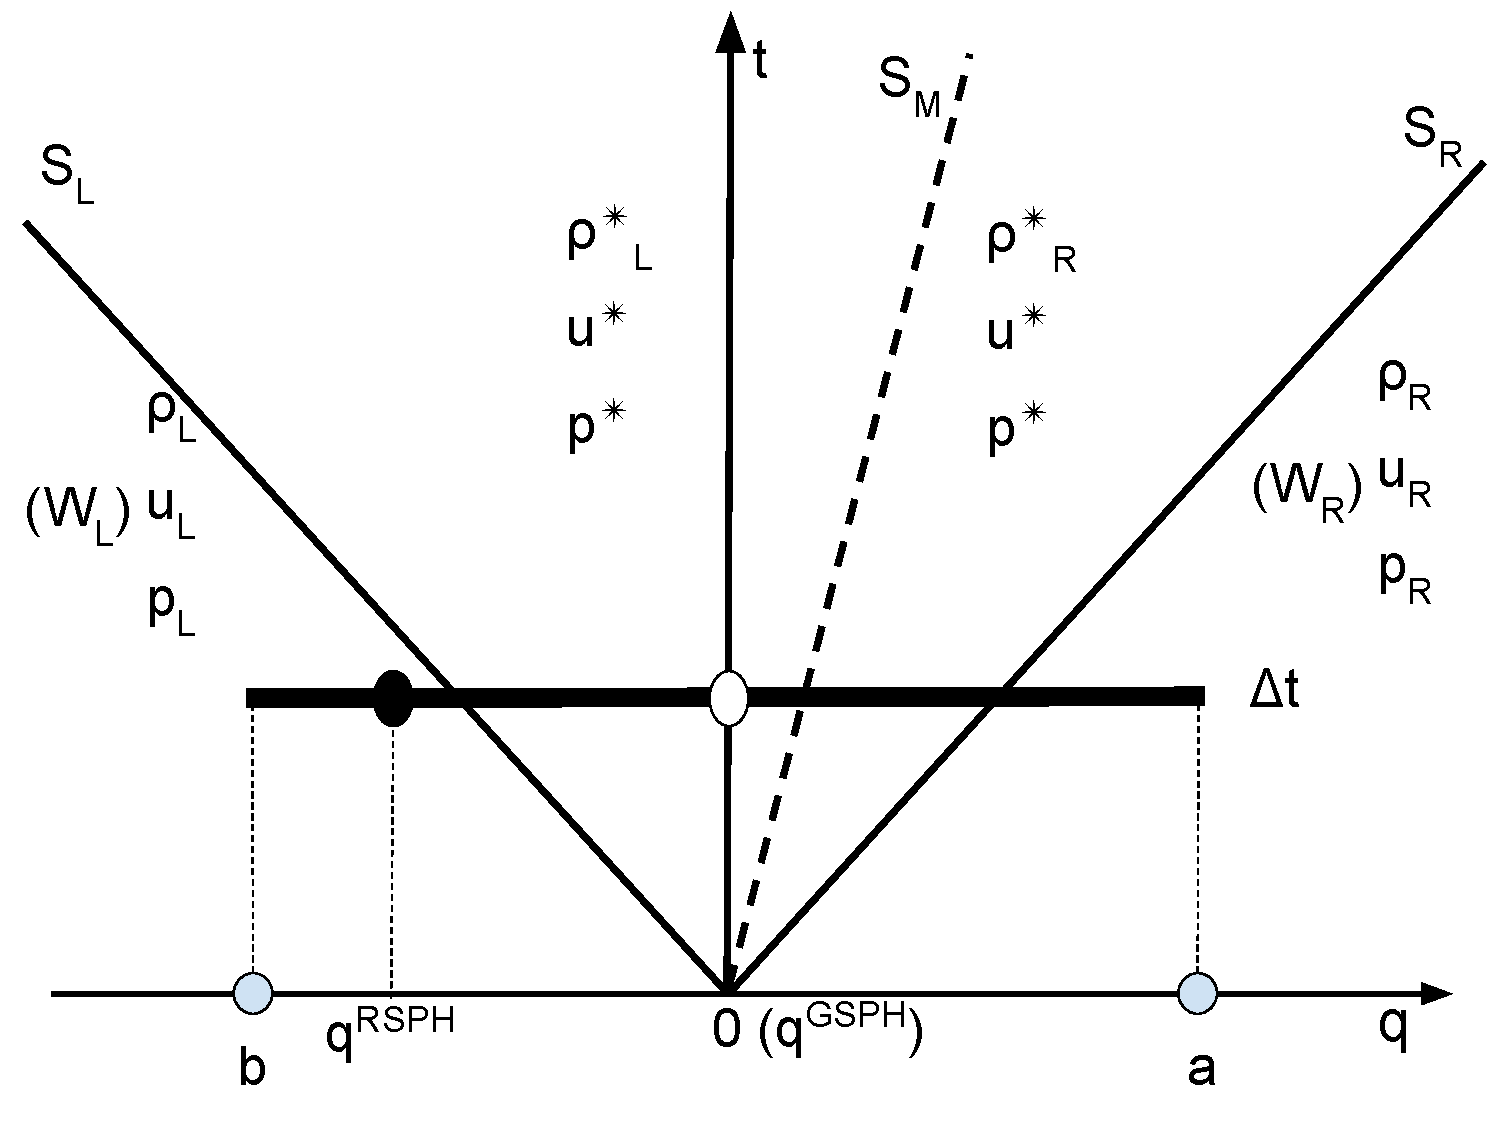
\includegraphics[width=0.5 \textwidth]{./Chapter-4/Figures/RSPH-GSPH}
    \caption{Evaluating of the starred state for  RSPH and GSPH implementations.
Particles are located at $\textbf{x}_{a} $ and $ \textbf{x}_{ b}$, and the local Riemann problem is defined by the constant states $(u, p)_a$ and $(u,p)_b$. The horizontal bold solid line at time $\Delta t$ indicates the interval on which to evaluate the solution of the Riemann problem. The dark ellipse is an example sample point of RSPH with the random number. The white ellipse indicates the stationary state, which is the starred state in GSPH.}
    \label{fig:pick-up-state-GSPH-RSPH}
\end{figure}

The starred state $(u^{\ast},  p^{\ast})$ must now be projected back into the global coordinate system, to define  $(\textbf{v}^{\ast},  p^{\ast})$.

We mention that, instead of selecting a uniformly distributed random number $\theta$, we follow \citet{colella1982glimm} and adopt the Van Der Corput pseudo-random number sequence \citep{hammersley2013monte}. See Appendix \ref{app:Van-Der-Corput-RDN} for more details.

\subsection{Non-iterative Riemann solvers} \label{sec:RP-solver}
Solving local Riemann problems exactly usually involves separating several cases of wave patterns and iteratively solving a small system of ordinary differential equations (for rarefaction waves) and a small set of nonlinear equations (the Rankine-Hugoniot equations). Instead of running this lengthy process one can employ approximate Riemann solvers, which provide an approximate solution quickly. There are many approximate Riemann solvers available \citep{rider1994review, luo2004computation, puri2014approximate}. For purposes here we adopt the HLLC solver, which decomposes the Riemann solution into 3 waves, including a (possible) contact discontinuity \cite{toro1994restoration}. More specifically, we adopt the HLLC formulation proposed by \citet{luo2004computation}.
 
We mention that, in the numerical tests in Section \ref{numericaltests}, Both the HLLC solver and Roe solver are used for GSPH calculations. Appendix \ref{app:RP-solvers} presents more details on these two approximate Riemann solver.
To summarize, our RSPH algorithm proceeds as follows:
\begin{itemize}
\item For each pair of particles, establish a local coordinate system whose axis joins the particles,
and project the primitive variables onto this local coordinate system to define left and right states;
\item Solve this local Riemann problem approximately using a HLLC solver;
\item Sample the solution using the Van Der Corput sequence, defining a state  $p^{\ast}, u^{\ast}$;
\item Project $p^{\ast}, u^{\ast}$  back to the global coordinate system, to obtain $p^{\ast}$ and $\textbf{v}^{\ast}$;
\item Update the particle positions and physical quantities.
\end{itemize}

\section{Numerical tests} \label{numericaltests}
We describe results from several numerical tests using SPH, RSPH and GSPH in this section.
A 1D shock tube tests is used to compare standard SPH, GSPH and RSPH. More shock tube simulations are also conducted to check the capacity of RSPH for different situations. In addition, order of accuracy is investigated for the 1D shock tube problem. In the last subsection we describe a 3D free jet flow simulation with SPH, GSPH and RSPH to check equivalent overall dissipation introduced by each method.

Six 1D simulations described here are carried out:
\begin{itemize}% [1D Tests]
\item Test 1 consists of a left rarefaction, a right traveling contact and a right shock. Density increases at down wind of contact wave. 
\item Test 2 also consists of a left rarefaction, a right traveling contact and a right shock. Density decreases at down wind of contact wave. 
\item Test 3 includes double expansion waves. The initial density is different at right and left hand side. 
\item Test 4 is a double shock tests with different initial density on the right side and left side.
\item Test 5 and Test 6 are two extreme cases. Test 5 is a cavity flow while test 6 is a strong blast flow.
\end{itemize}

\begin{table}
\centering
      \caption{Overview of 1D shock tube tests}		
	  \begin{tabular}{lrrrrrrrrrr}
	    \hline
	          & $\rho_L$ & $p_L$ &$v_L$ & $\rho_R$ & $p_R$ &$v_R$ & $m$ & $[x_L, x_R]$ & $t_f$\\
	    \hline
	    Test 1 & $1.0$ & $1.0$ &$0$ & $0.25$ & $0.1795$ &$0$ & $0.003$  & $[-0.4, 0.4]$ & $0.17$\\
	    	Test 2 & $1.0$ & $1.0$ &$0$ & $0.5$ & $0.2$ &$0$ & $0.003$  & $[-0.4, 0.4]$ & $0.2$\\
	    	Test 3 & $2.0$ & $1.95$ &$1.0$ & $1.0$ & $1.95$ &$-1.0$  & $0.006$  & $[-0.4, 0.4]$ & $0.13$\\
	    Test 4 & $1.0$ & $2.4$ &$8.0$ & $0.5$ & $0.4$ &$-0.25$ & $0.003$  & $[-0.4, 0.4]$ & $0.05$\\
	    	Test 5 & $1.0$ & $-2.0$ &$0.4$ & $1.0$ & $0.4$ &$2.0$ & $0.003$  & $[-0.4, 0.4]$ & $0.18$\\
	    	Test 6 & $1.0$ & $0$ &$1000$ & $1.0$ & $0$ &$0.01$ & $0.003$  & $[-0.5, 0.5]$  & $0.01$\\
	    \hline
	  \end{tabular}
	  \label{tab:1D-shock-input_parameters}
\end{table}
Input parameters for 1D tests can be found in Table \ref{tab:1D-shock-input_parameters}, where, subscript $L$ refers left side and $R$ for right side. $m$ is particle mass, initial interval between adjacent particles are adjusted to guarantee equal particle mass. $t_f$ is the time to terminate simulation and plotting the results. Equal particle mass is assigned to all particles. The $x$ axis in all plots is normalized by time, that is $x/t_f$, in plots for shock tube tests results.
\subsection{Comparison of RSPH with standard SPH and GSPH}
\begin{figure}
    \centering
    \begin{minipage}{.495\textwidth}
        \centering a)
        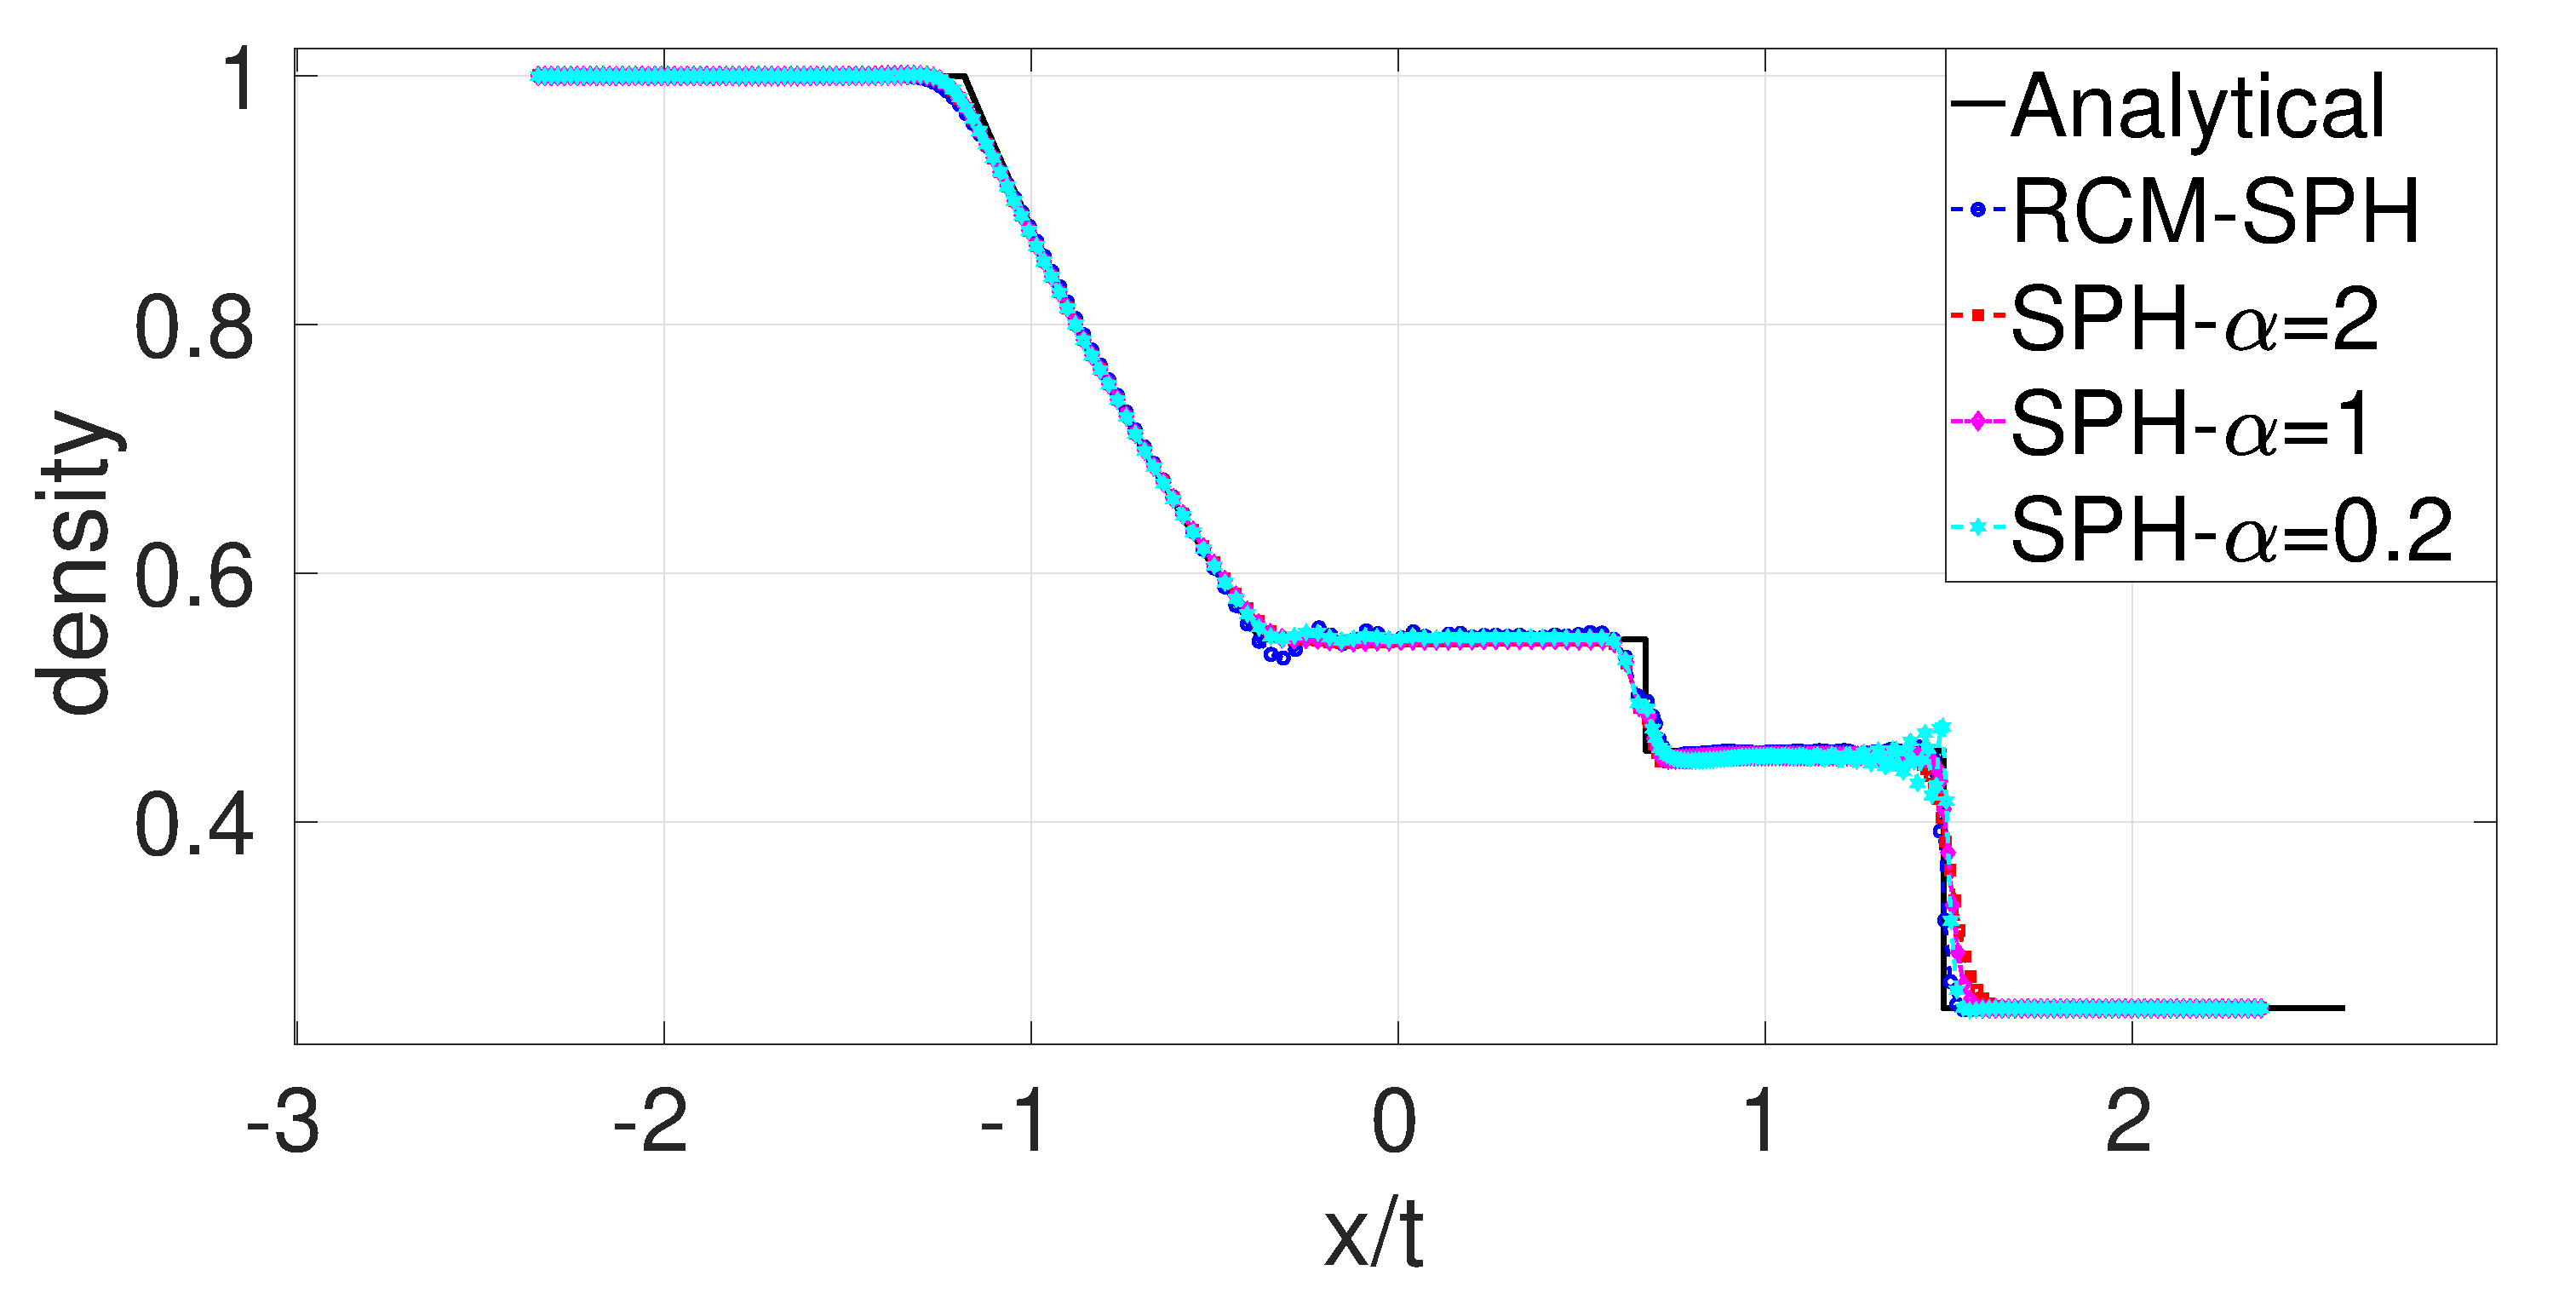
\includegraphics[width=0.99 \textwidth,height=0.7\textwidth]{./Chapter-4/Figures/Sod/RCM-Sod-SPH-alf-rho}
    \end{minipage}%
    \begin{minipage}{.495 \textwidth}
        \centering b)
        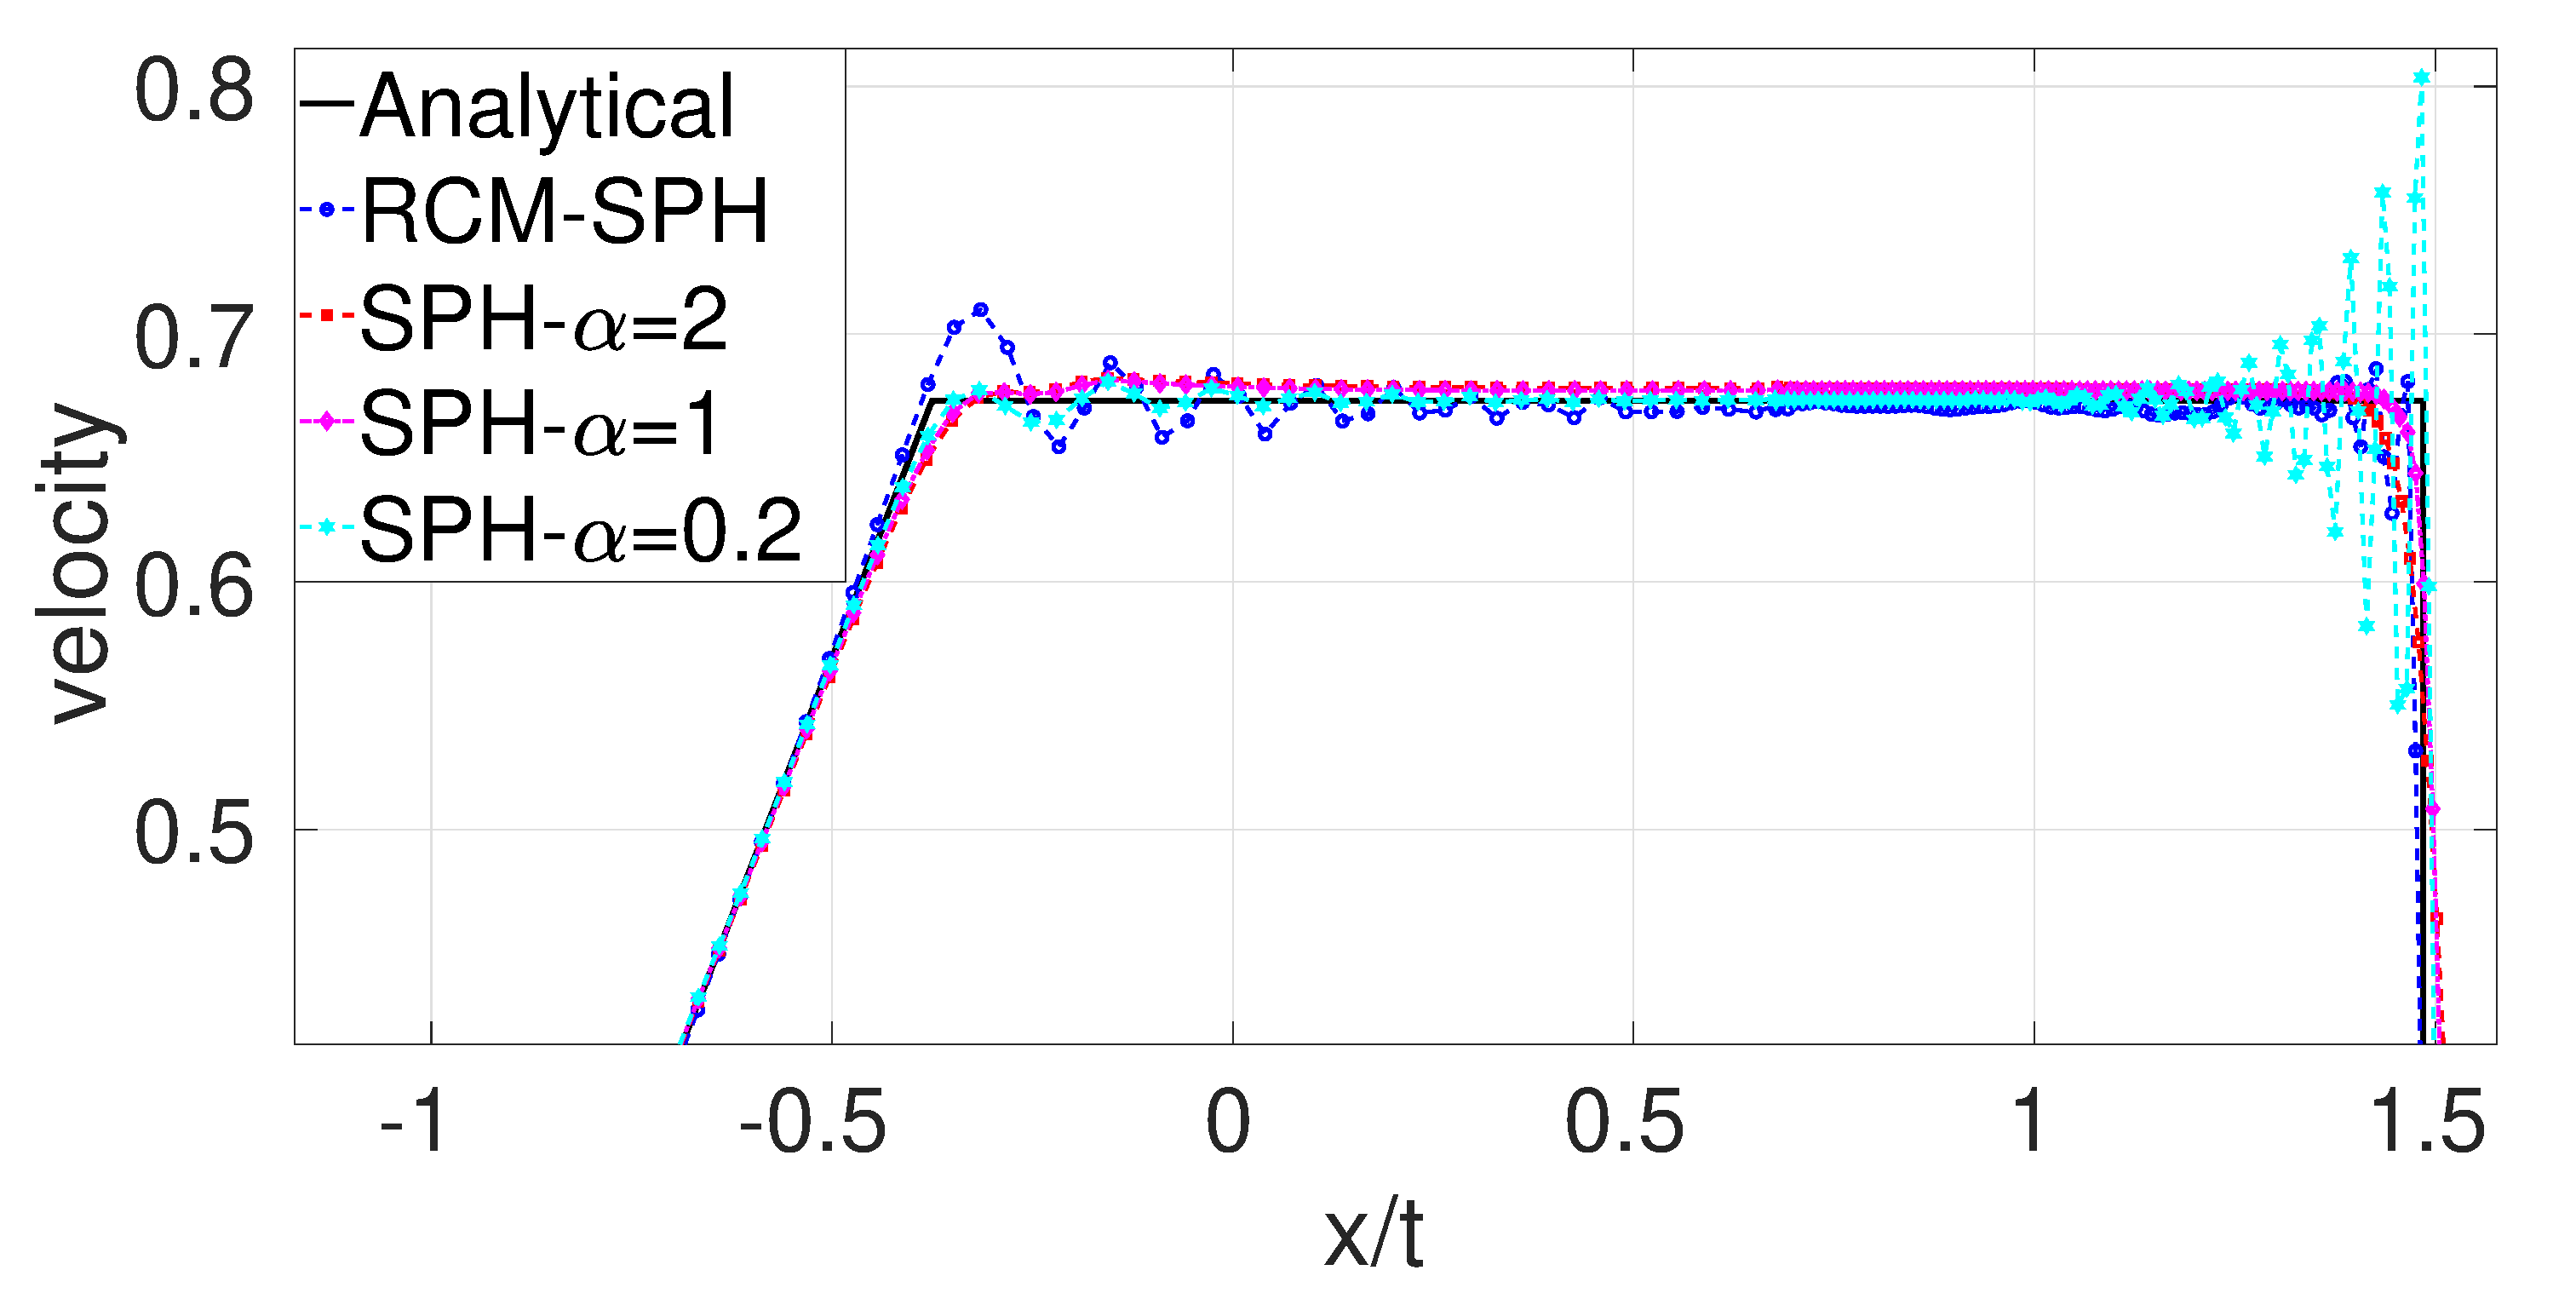
\includegraphics[width=0.99 \textwidth,height=0.7\textwidth]{./Chapter-4/Figures/Sod/RCM-Sod-SPH-alf-v}
    \end{minipage}%
    \\
    \begin{minipage}{.495\textwidth}
        \centering c)
        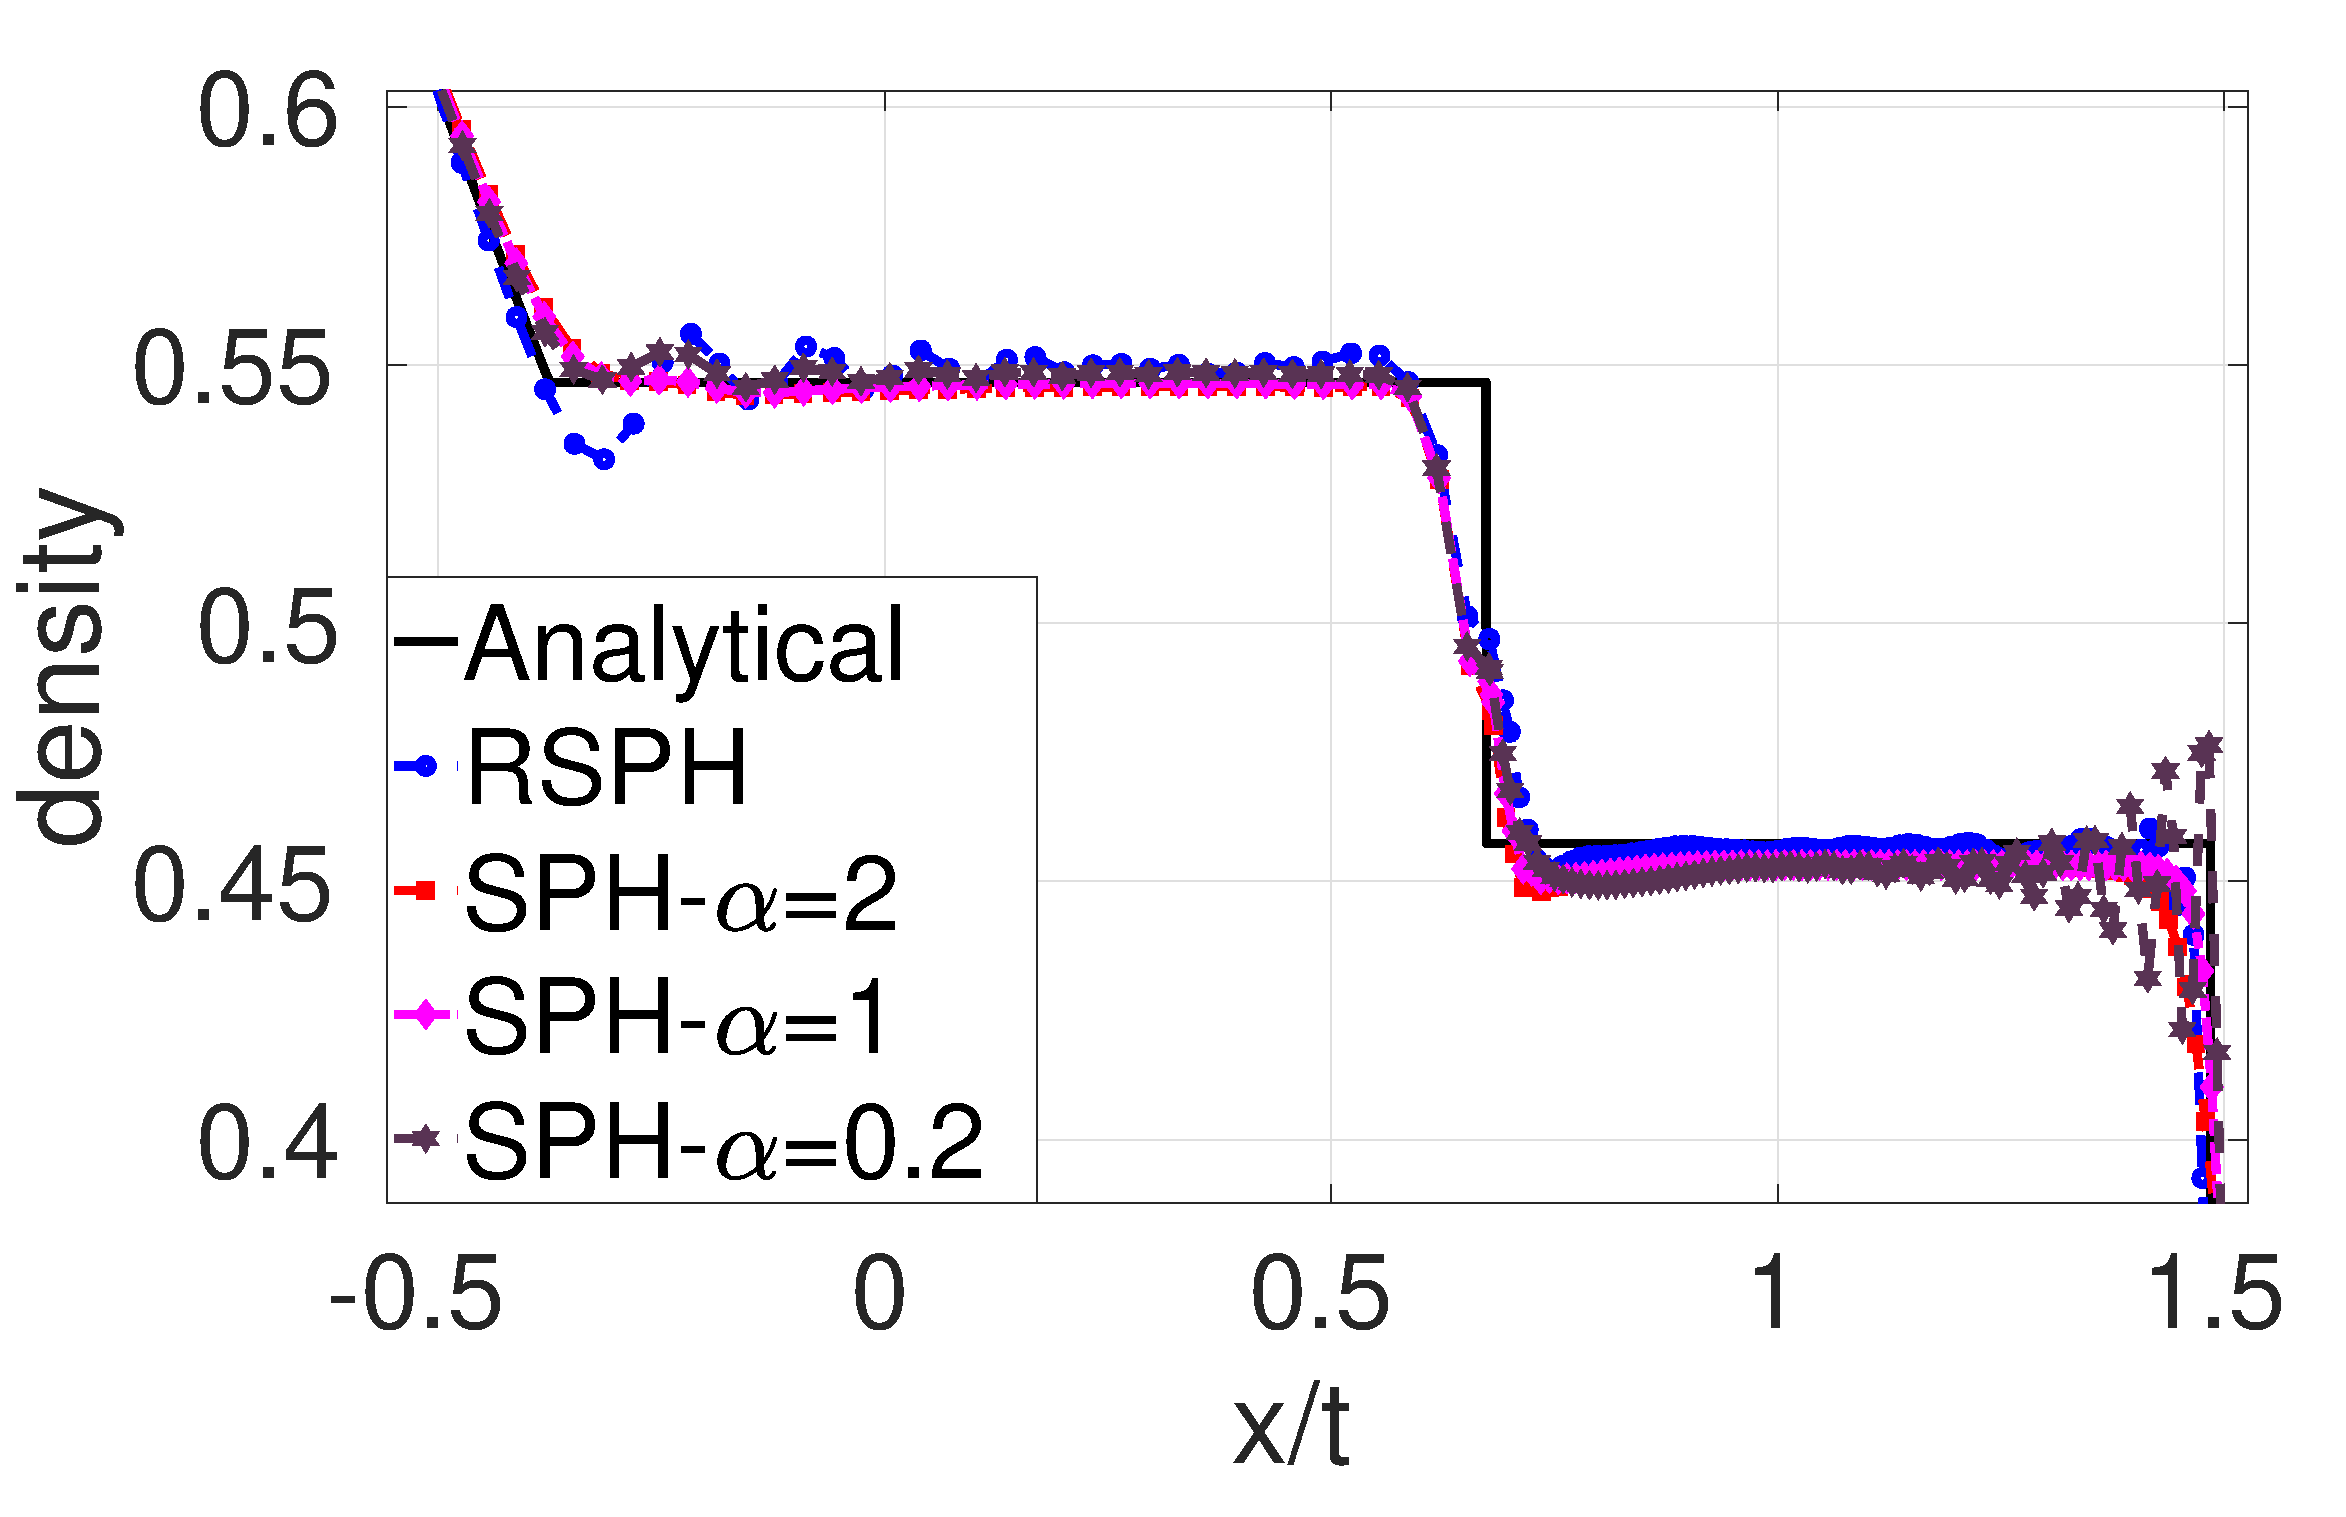
\includegraphics[width=0.99 \textwidth,height=0.7\textwidth]{./Chapter-4/Figures/Sod/RCM-Sod-SPH-alf-rho-zoom}
    \end{minipage}%
    \begin{minipage}{.495 \textwidth}
        \centering d)
        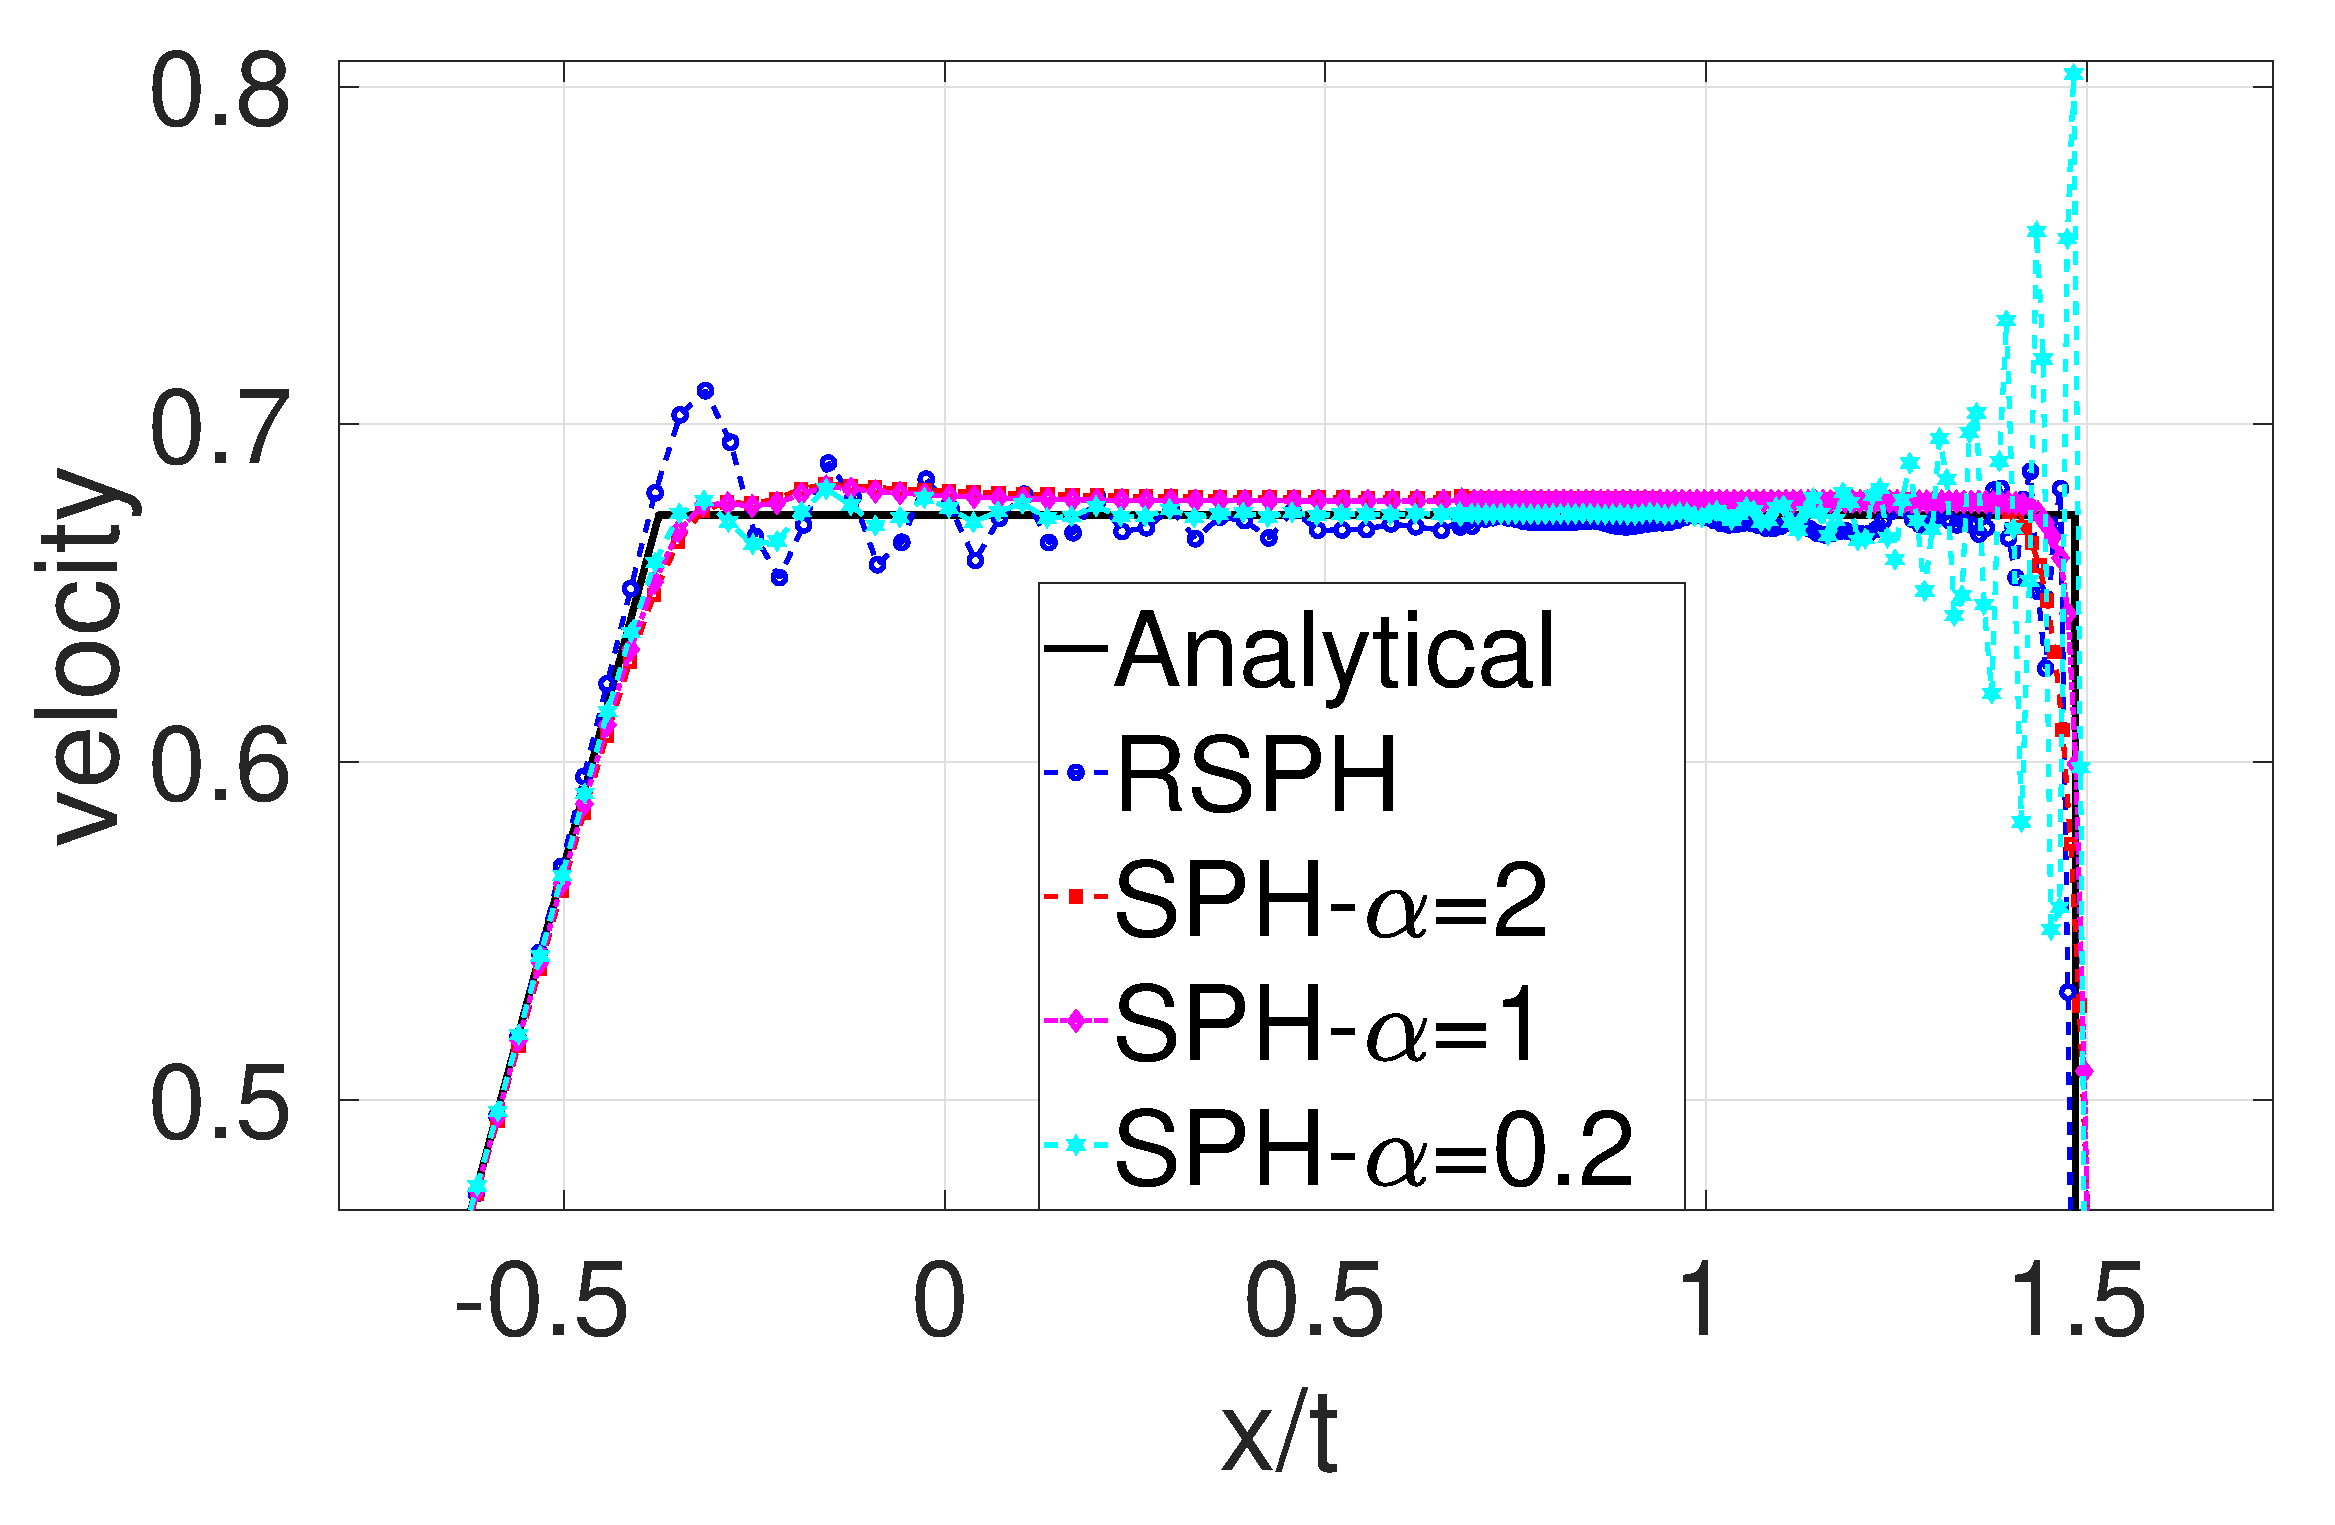
\includegraphics[width=0.99 \textwidth,height=0.7\textwidth]{./Chapter-4/Figures/Sod/RCM-Sod-SPH-alf-v-zoom}
    \end{minipage}%   
    \caption{a),b) are simulation results of density and velocity in Test 1 by RSPH and SPH with different artificial viscosity coefficients $\alpha,\beta$ satisfying: $\beta=2\alpha$.  c), d) are zoomed views, showing that $\alpha=0.2$ provided insufficient viscosity to suppress oscillations around shock. The dissipation introduced by RSPH. on the other hand, is adaptive, introducing more damping at the shock (comparable to $\alpha=1.0$) and less damping in the area away from the shock (less than $\alpha=0.2$, as indicated by the magnitude of oscillation).}
    \label{fig:RCM-Sod-SPH-alf}
\end{figure}

\begin{figure}
    \centering
    \begin{minipage}{.495\textwidth}
        \centering a)
        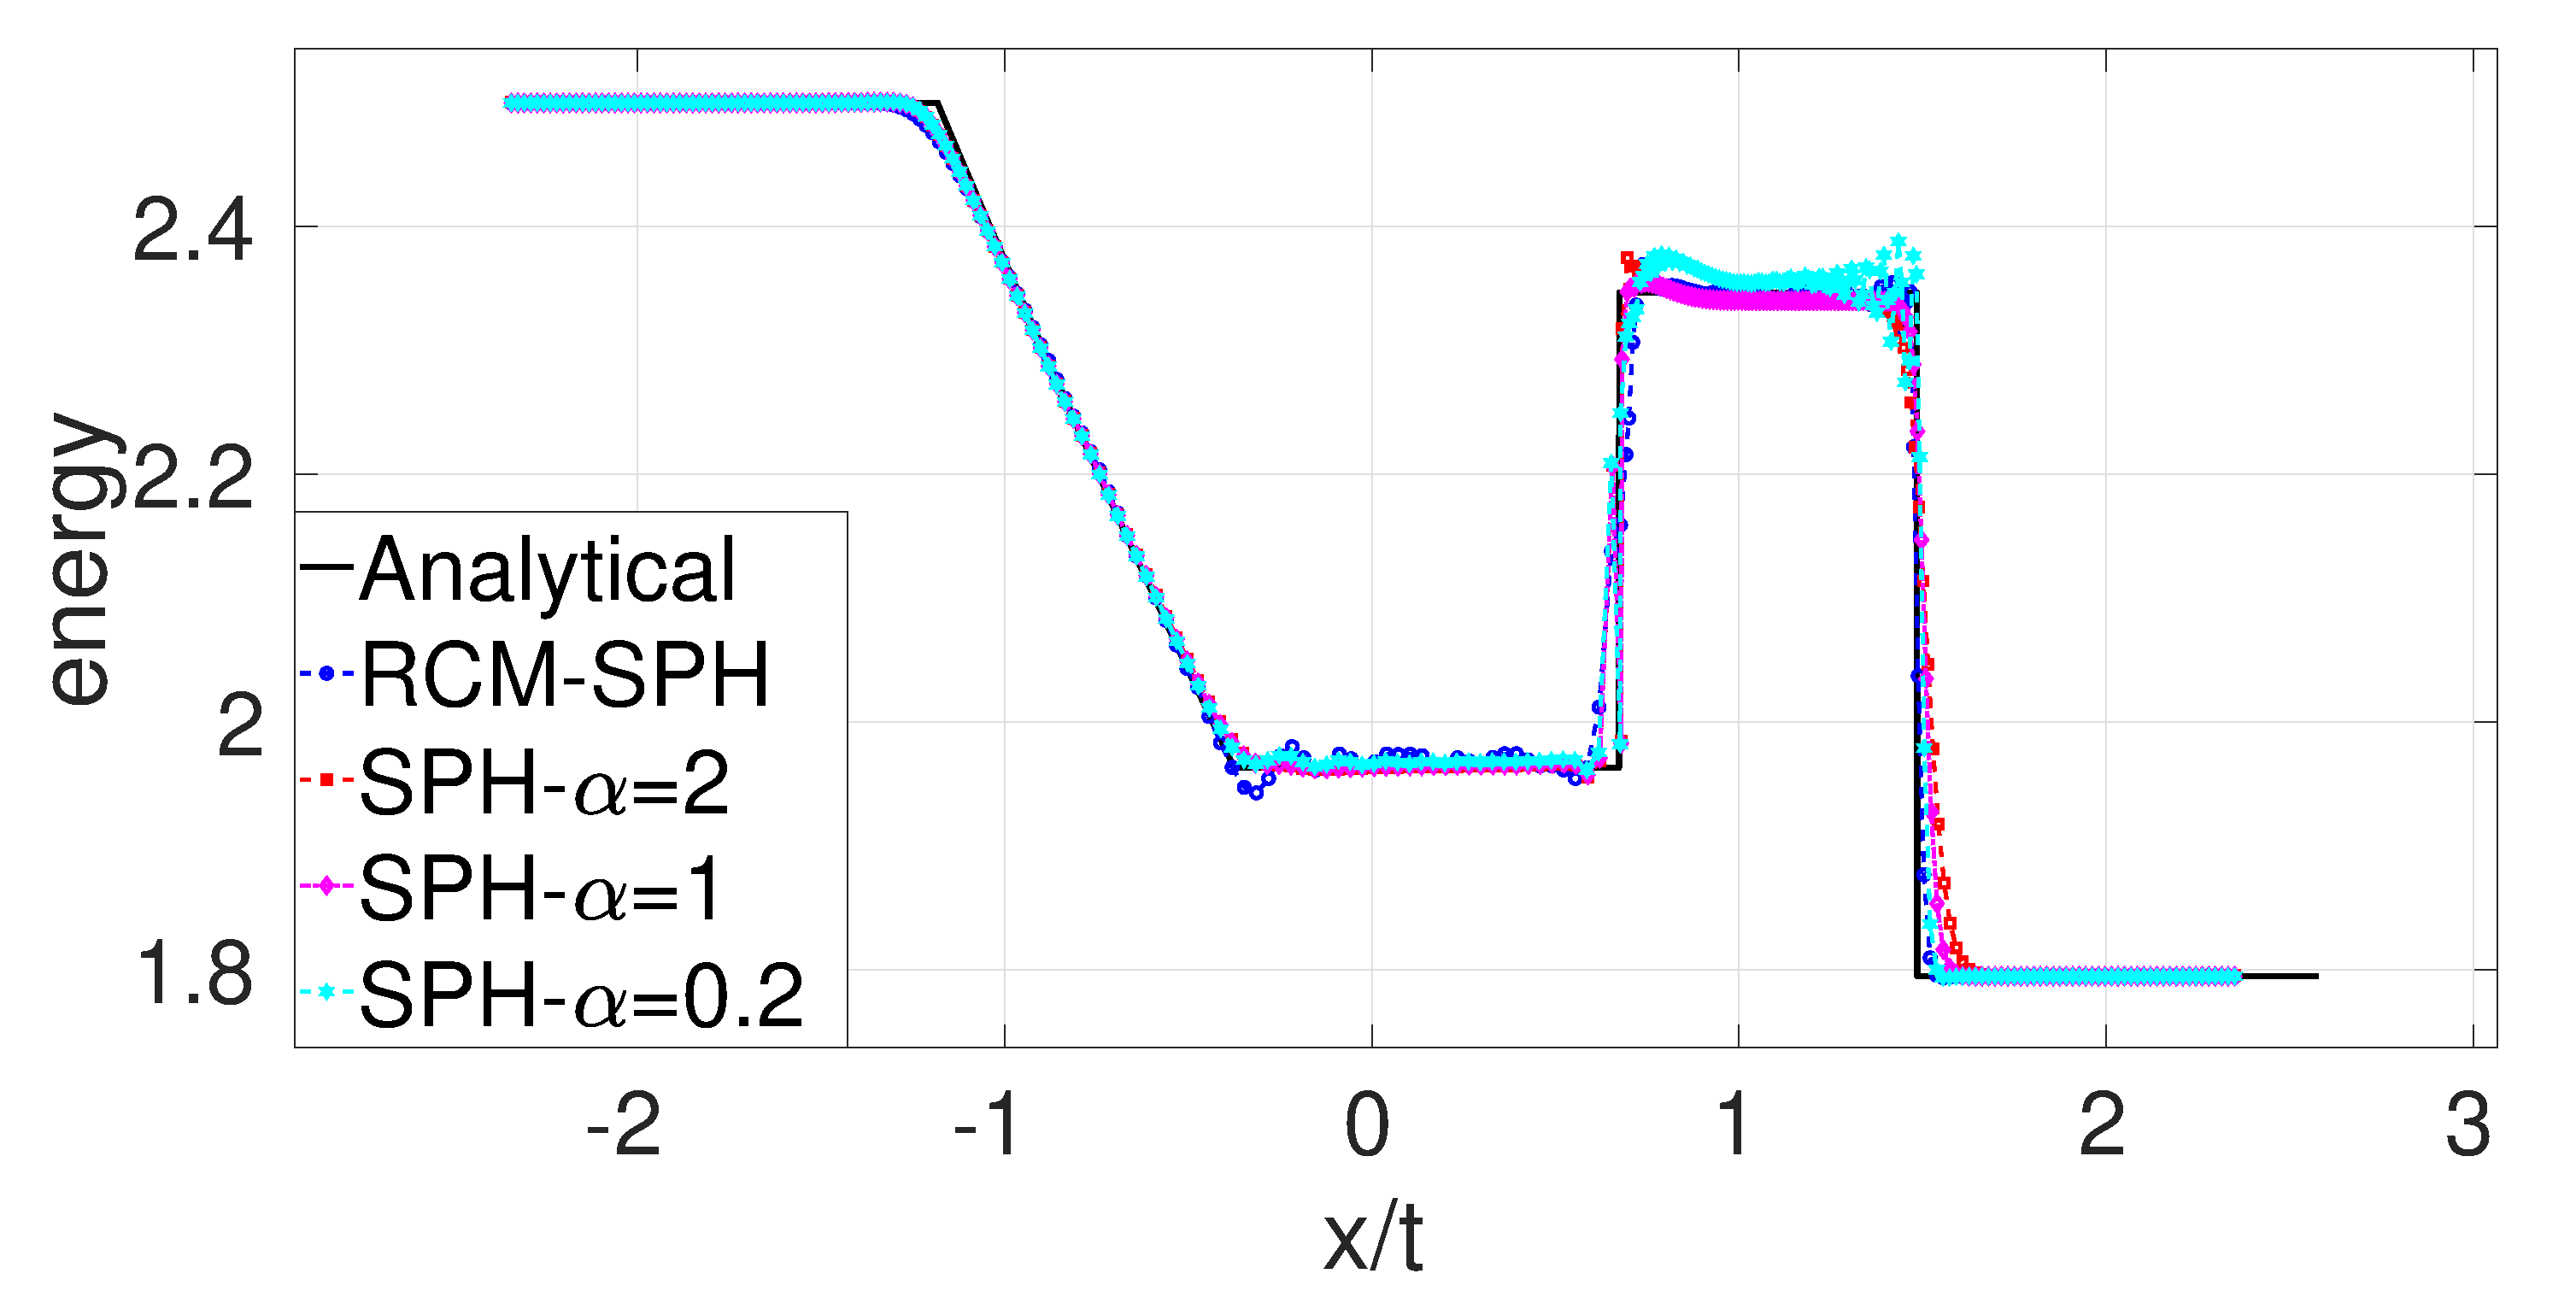
\includegraphics[width=0.99 \textwidth,height=0.7\textwidth]{./Chapter-4/Figures/Sod/RCM-Sod-SPH-alf-e}
    \end{minipage}%
    \begin{minipage}{.495 \textwidth}
        \centering b)
        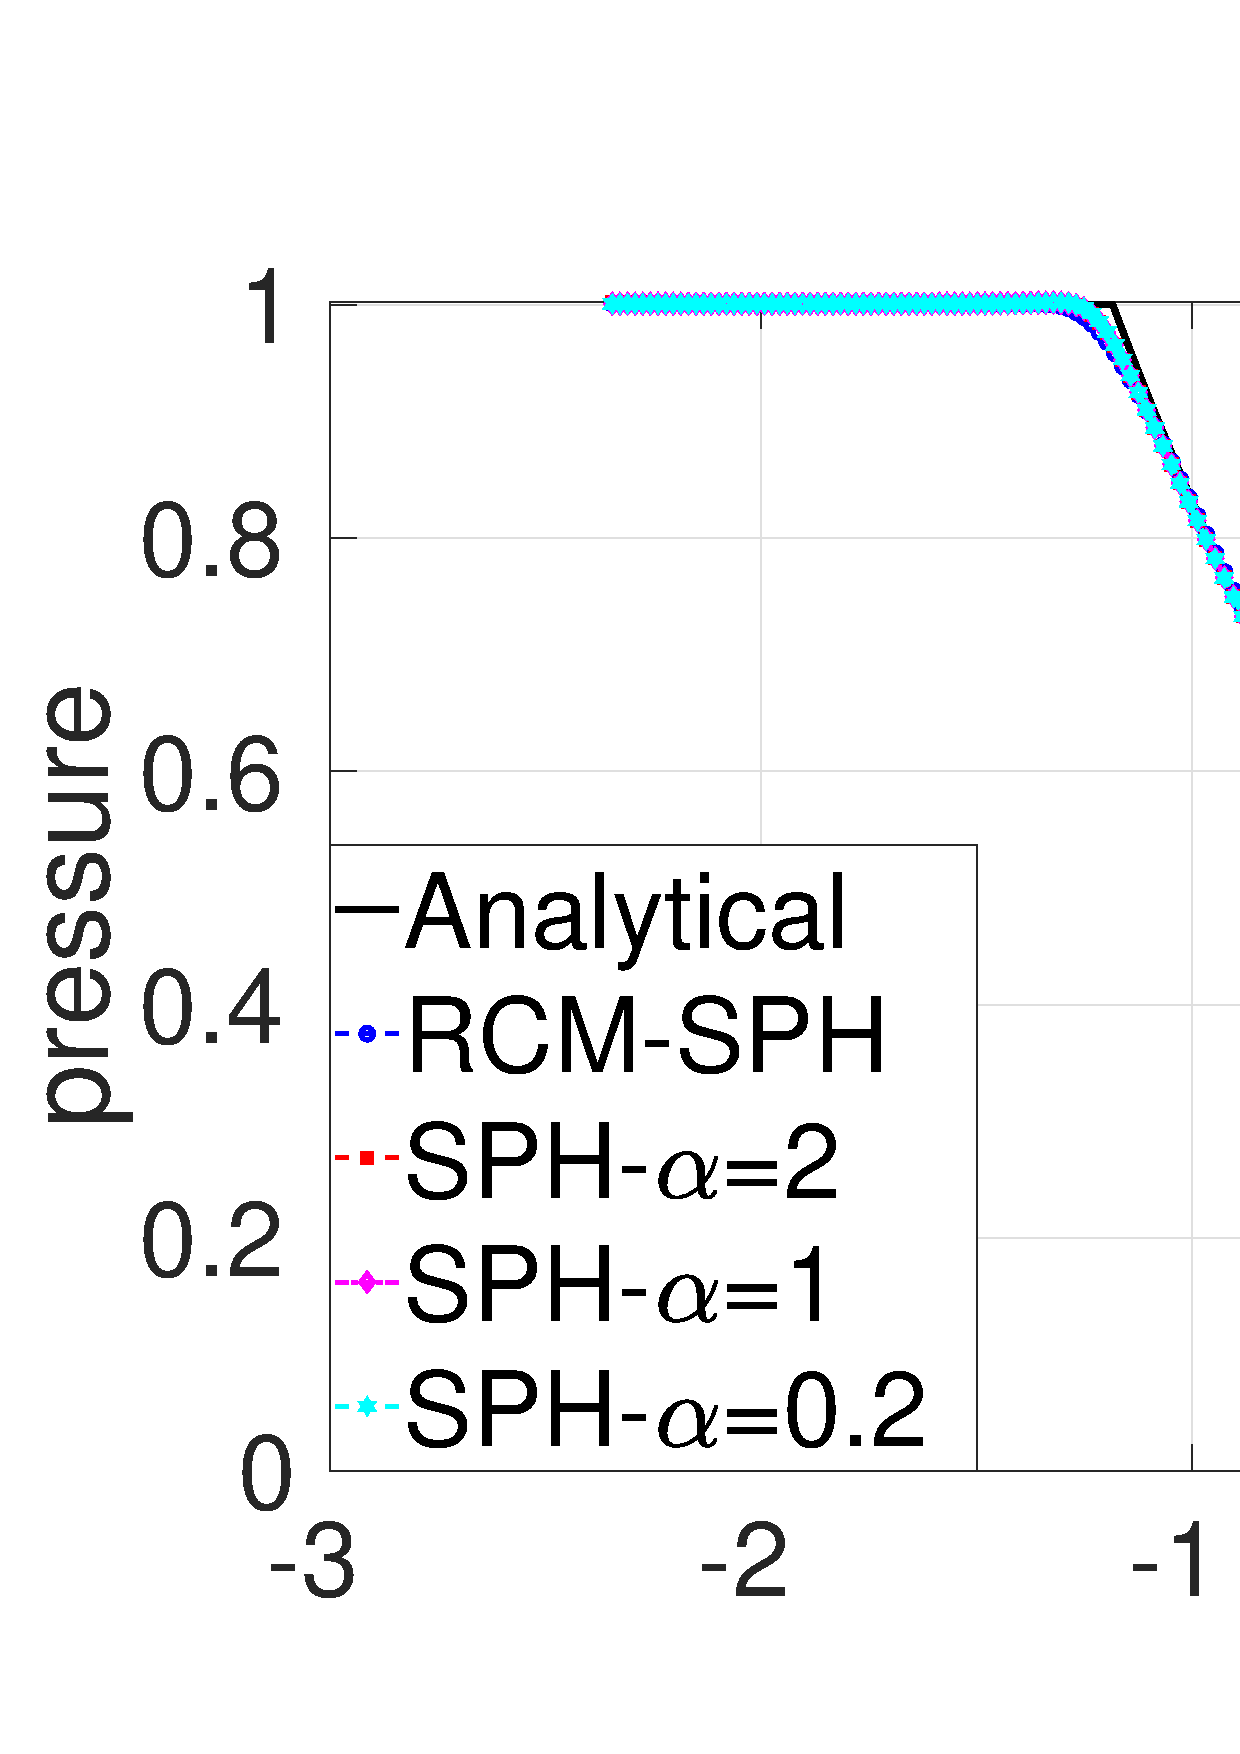
\includegraphics[width=0.99 \textwidth,height=0.7\textwidth]{./Chapter-4/Figures/Sod/RCM-Sod-SPH-alf-p}
    \end{minipage}% 
    \\
    \begin{minipage}{.495 \textwidth}
        \centering c)
        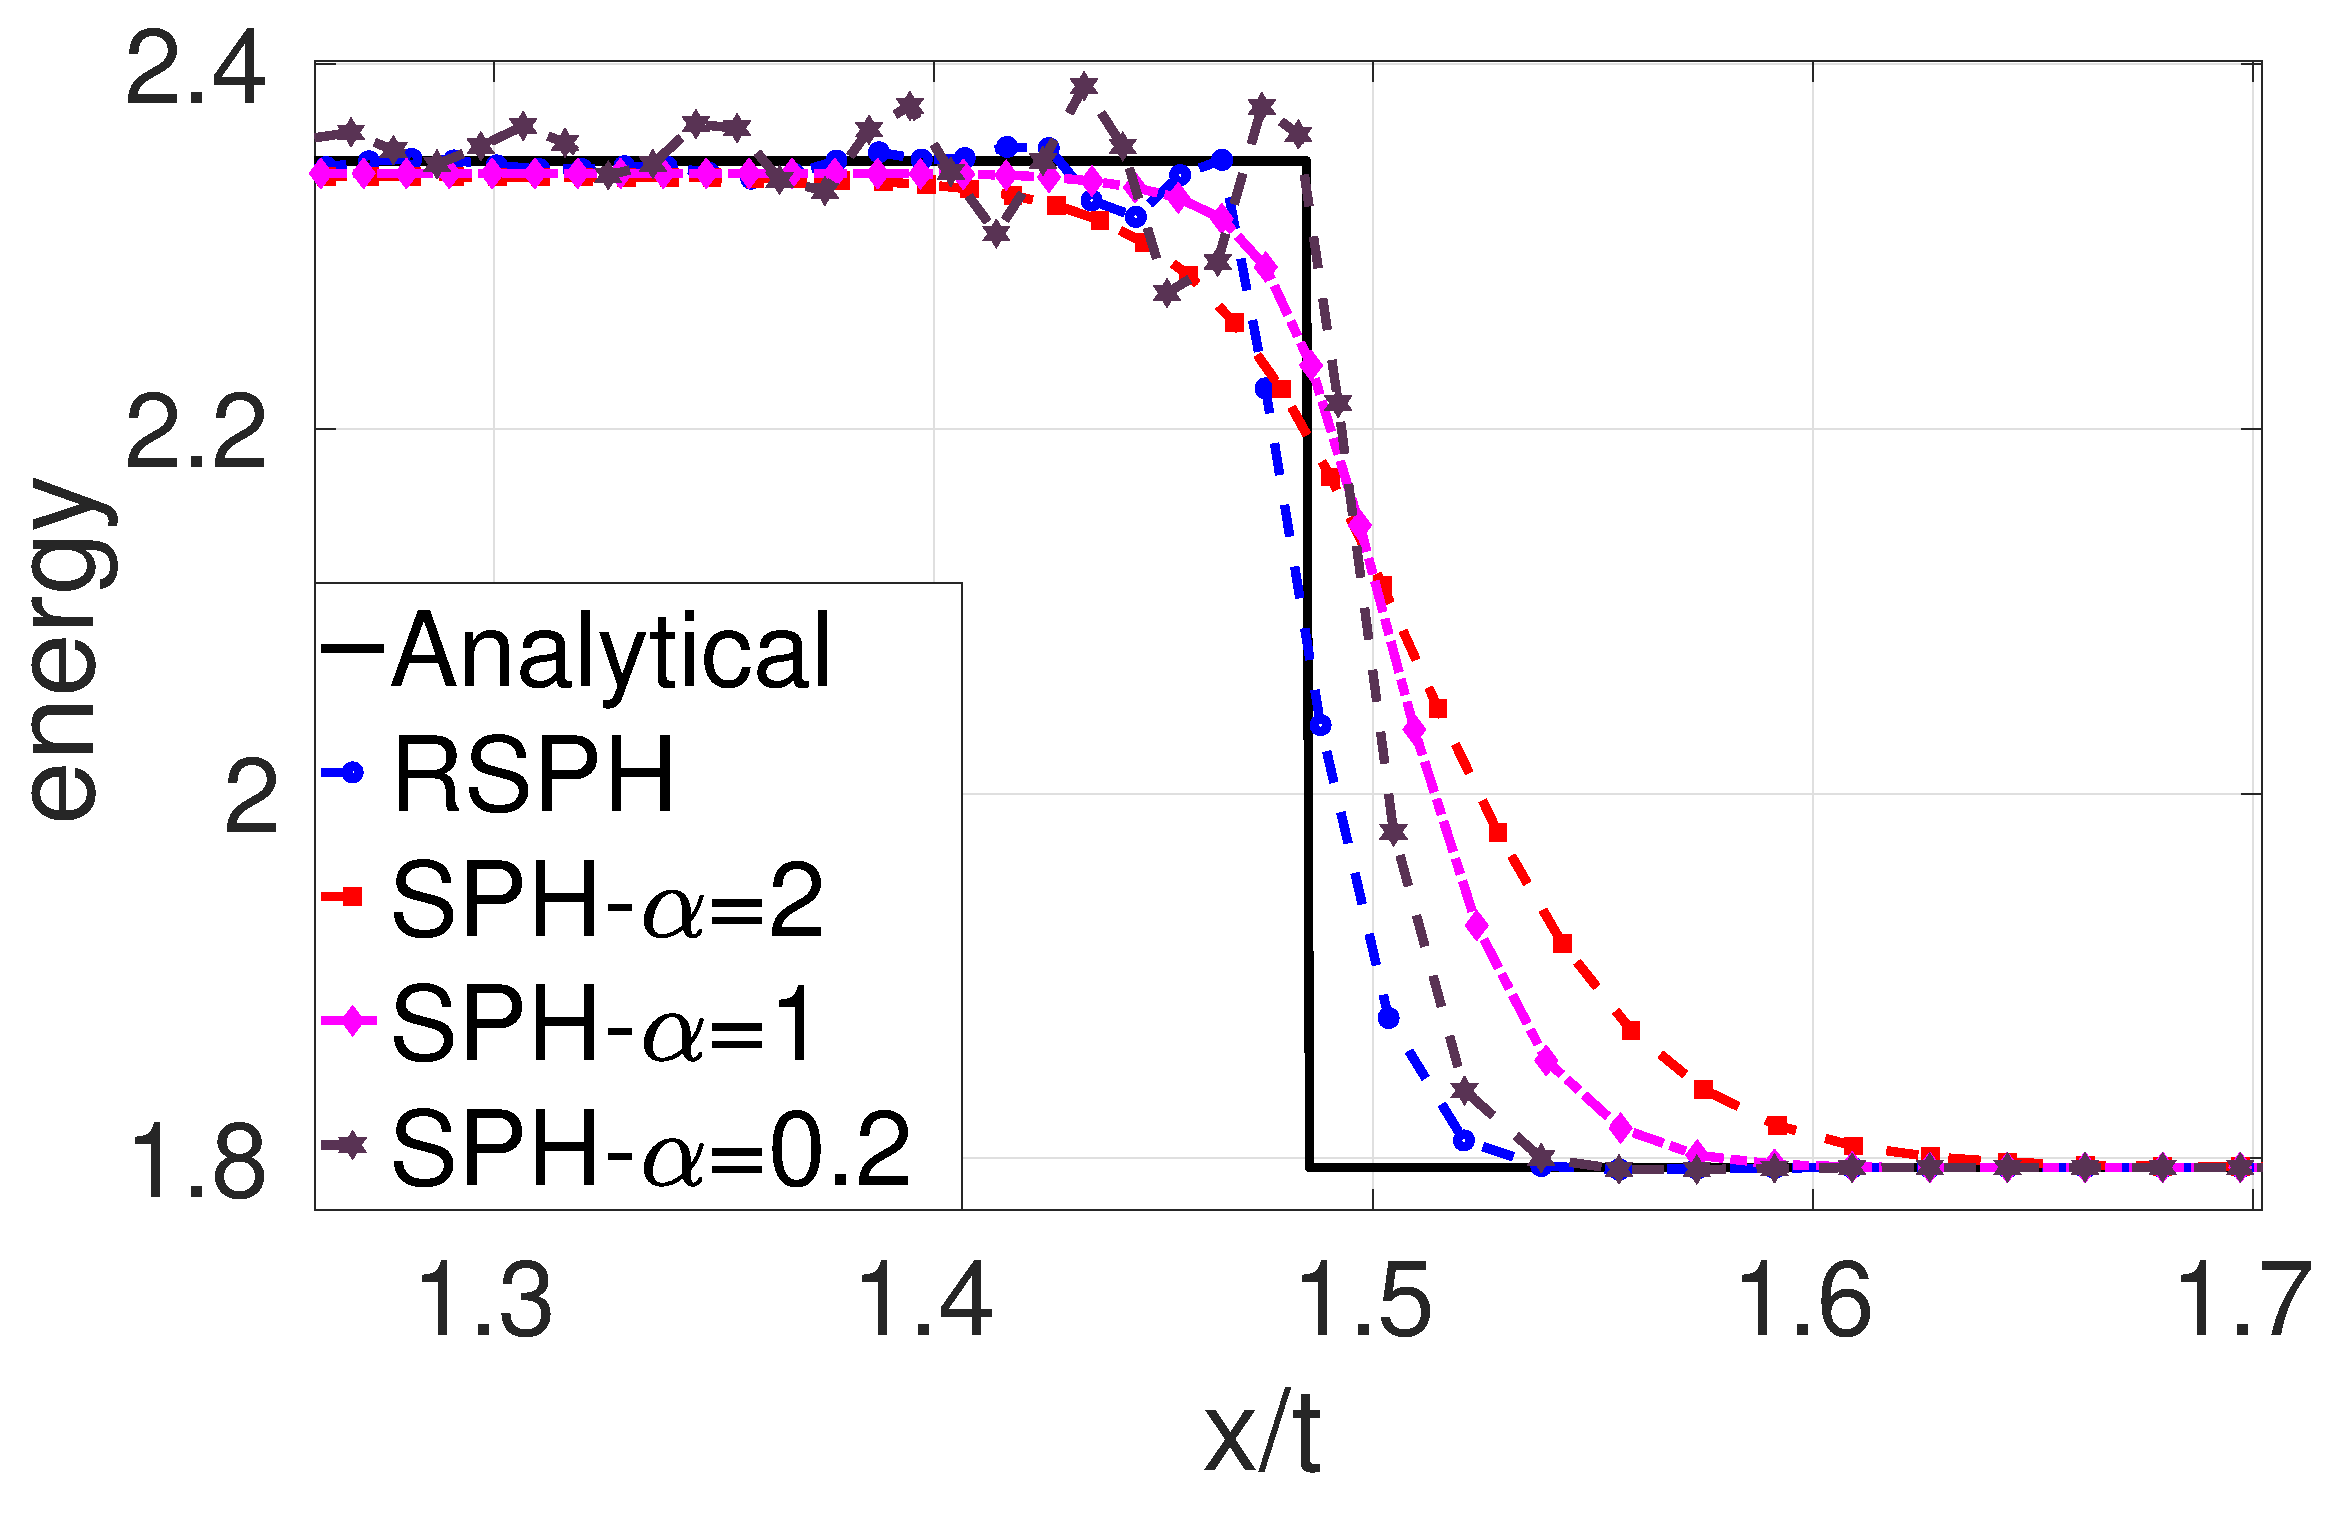
\includegraphics[width=0.99 \textwidth, height=0.7\textwidth]{./Chapter-4/Figures/Sod/RCM-Sod-SPH-alf-e-zoom}
    \end{minipage}% 
    \begin{minipage}{.495\textwidth}
        \centering d)
        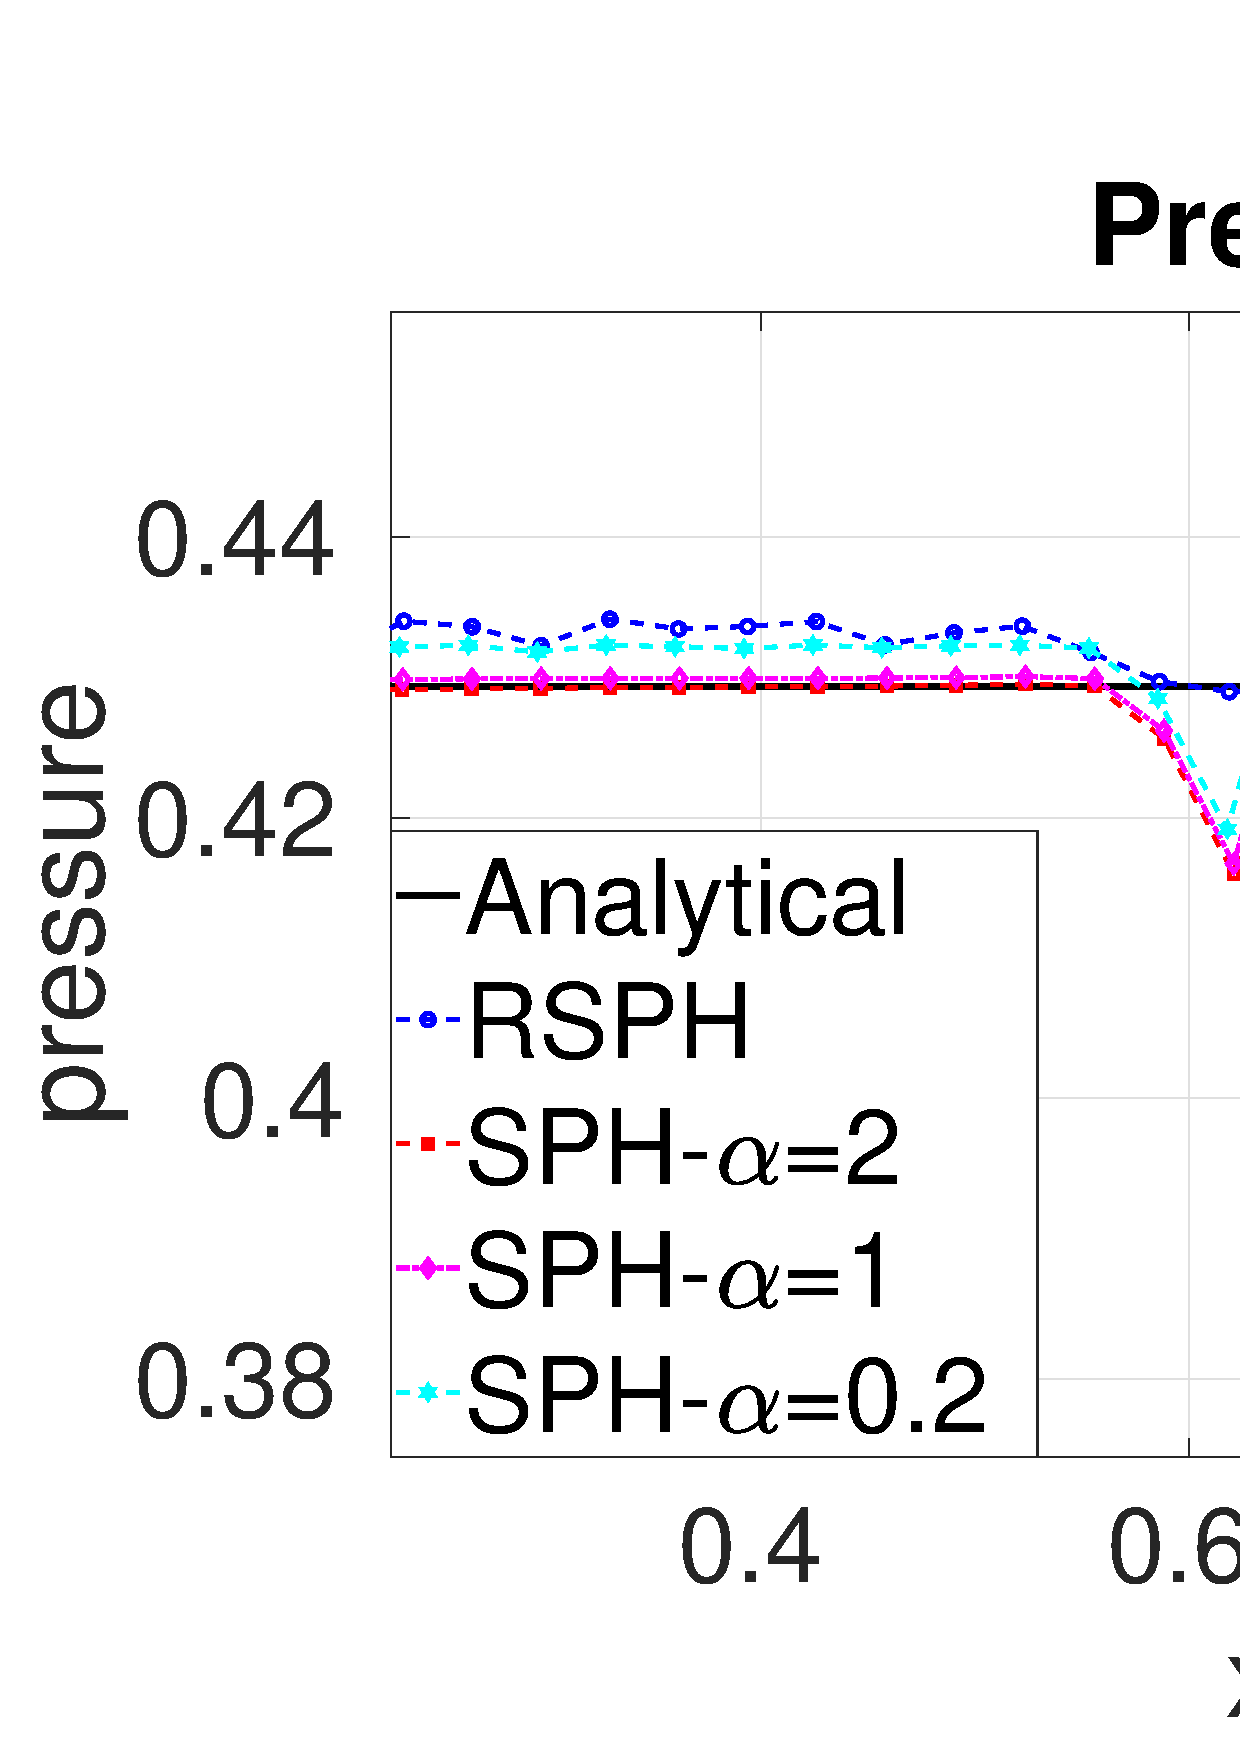
\includegraphics[width=0.99 \textwidth, height=0.7\textwidth]{./Chapter-4/Figures/Sod/RCM-Sod-SPH-alf-p-zoom}
    \end{minipage}%    
    \caption{
    a),b) are simulation results of internal energy and pressure in Test 1 by RSPH and SPH with different artificial viscosity coefficients $\alpha,\beta$ satisfying: $\beta=2\alpha$.  c), d) are zoomed views.  For $\alpha=1$ and $\alpha=2$, as shown in c), numerical oscillations are completely suppressed though the shock is now smeared. $\alpha=0.2$ provided insufficient viscosity to suppress oscillations. Comparing RSPH and SPH shows that RSPH is adaptive, more dissipative at the shock (comparable or better than $\alpha=1.0$) and less dissipative away from the shock (less than $\alpha=0.2$). d) shows pressure around the contact discontinuity. It is evident that RSPH gets rid of the pressure ``wiggle" around the contact discontinuity.}
    \label{fig:RCM-Sod-SPH-alf-zoom}
\end{figure}

Test 1 is simulated using standard SPH with different artificial viscosity coefficients, GSPH and RSPH. The comparison between RSPH and SPH using different artificial viscosity coefficients is shown in Fig. \ref{fig:RCM-Sod-SPH-alf} and \ref{fig:RCM-Sod-SPH-alf-zoom}. In all simulations, the artificial viscosity coefficient $\beta$ is set to be twice of $\alpha$. For example, for the test ``$SPH-\alpha=2$", $\beta=4$. Several interesting observation are made based on the comparison between SPH and RSPH. The effect of artificial viscosity is illustrated through comparison.
First of all, dissipation (introduced by artificial viscosity in these tests) decays the numerical fluctuations. Numerical fluctuations are suppressed completely when large enough dissipation is introduced, for example, by using sufficiently large artificial viscosity coefficients ($\alpha=1,2$).
Secondly, the equivalent artificial viscosity introduced by RSPH varies adaptively.
As shown in Fig. \ref{fig:RCM-Sod-SPH-alf} and \ref{fig:RCM-Sod-SPH-alf-zoom}, RSPH assigns smaller artificial viscosity  (equivalent $\alpha$ much less then 0.2) at the area far away from shock and sufficiently large artificial viscosity coefficients (equivalent $\alpha$ is about 1.0) around the shock. So RSPH is actually more adaptive than SPH. This feature is very desirable not only because it could eliminate parameterization and hence user intervention associated with artificial viscosity coefficients but also because it avoids introducing excess artificial viscosity.
Thirdly, RSPH introduces less smearing of the shock discontinuity compared with SPH using most commonly adopted artificial viscosity coefficients ($\alpha=1.0$, $\beta=2.0$). Recall that RCM is able to resolve discontinuities as true discontinuity. RSPH, even though it still smears the discontinuity in some degree, introduces much less smearing (see Fig. \ref{fig:RCM-Sod-SPH-alf-zoom}).
The last but not the least, the pressure ``wiggle" around contact discontinuity is completely eliminated by RSPH as seen in Fig. \ref{fig:RCM-Sod-SPH-alf-zoom}. It has been shown that thermal conduction is essential to mitigate the spurious pressure ``wiggle" at contact discontinuity in SPH \citep{monaghan1997sph, sigalotti2006shock, price2008modelling, price2012smoothed}. As for GSPH, it is reported that an implicit thermal conduction is introduced by Godunov's scheme and helps suppress the anomaly \citep{puri2014approximate}. Even though, the ``wiggle" still visible in pressure distribution and velocity distribution of GSPH simulation results (for example, see figures in \citep{puri2014comparison}) and RSPH simulation results of other tests (see section \ref{sec:comprehensive-1d-tests}). ``Wiggle" in test 1, however, is completely eliminated by both GSPH and RSPH.

\begin{figure}
    \centering
    \begin{minipage}{.495\textwidth}
        \centering
        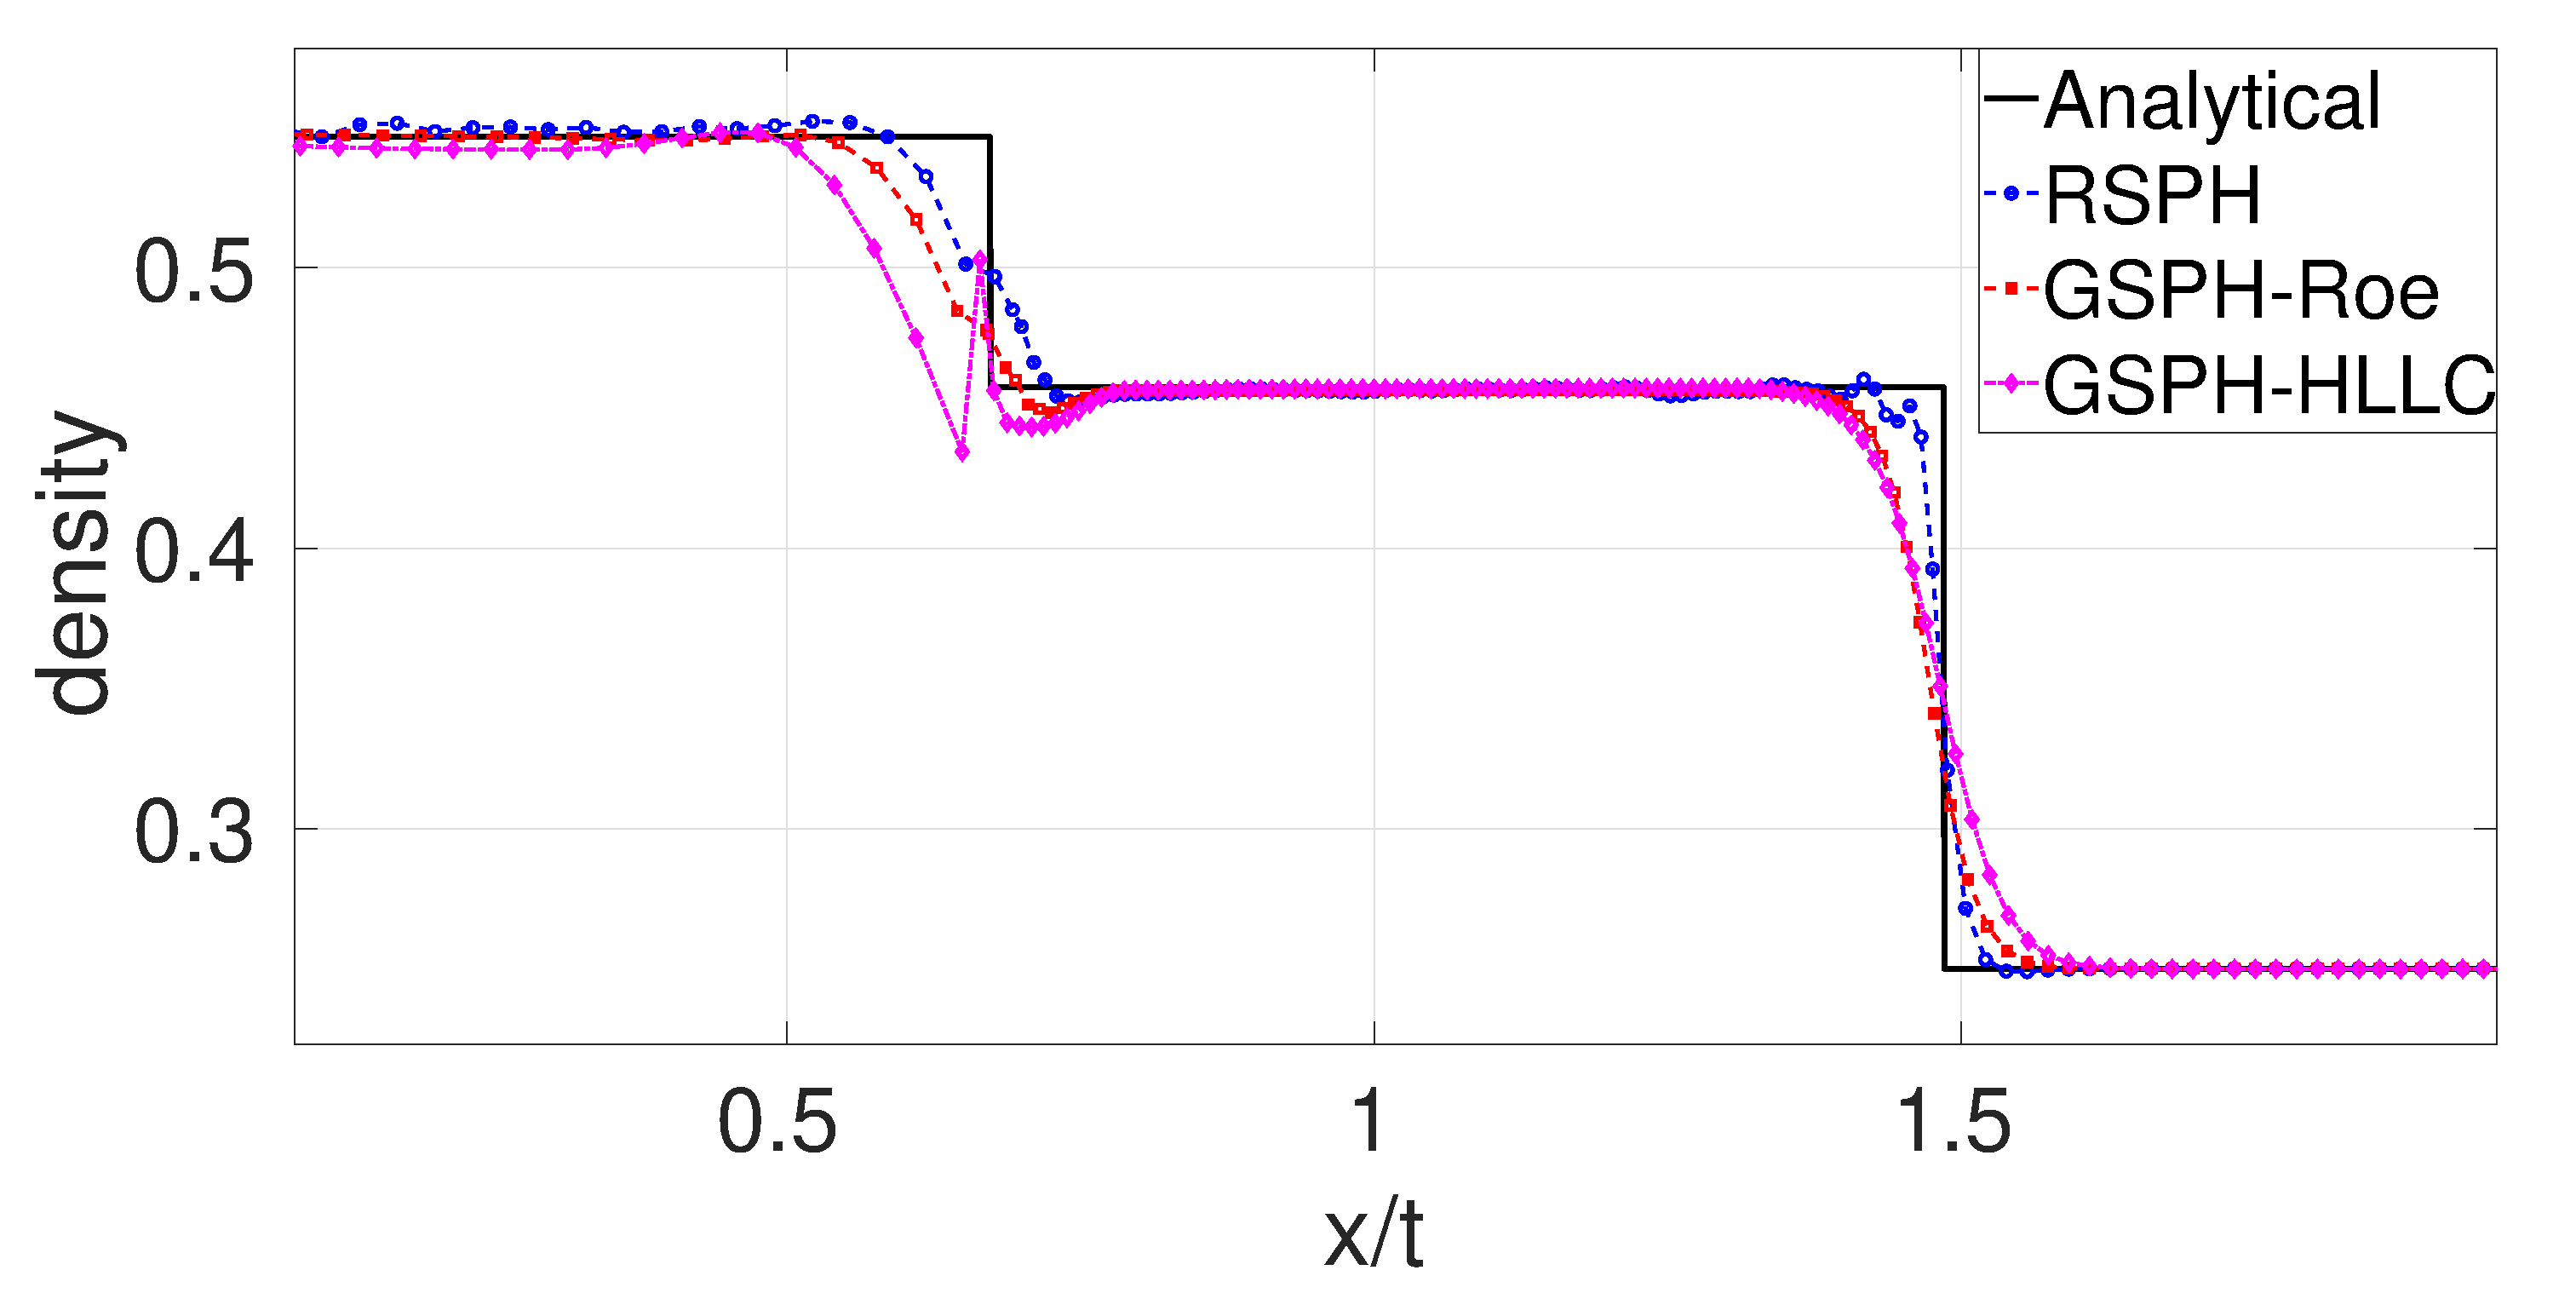
\includegraphics[width=0.99 \textwidth,height=0.6\textwidth]{./Chapter-4/Figures/Sod/RCM-Sod-GSPH-compare-rho}
    \end{minipage}%
    \begin{minipage}{.495 \textwidth}
        \centering
        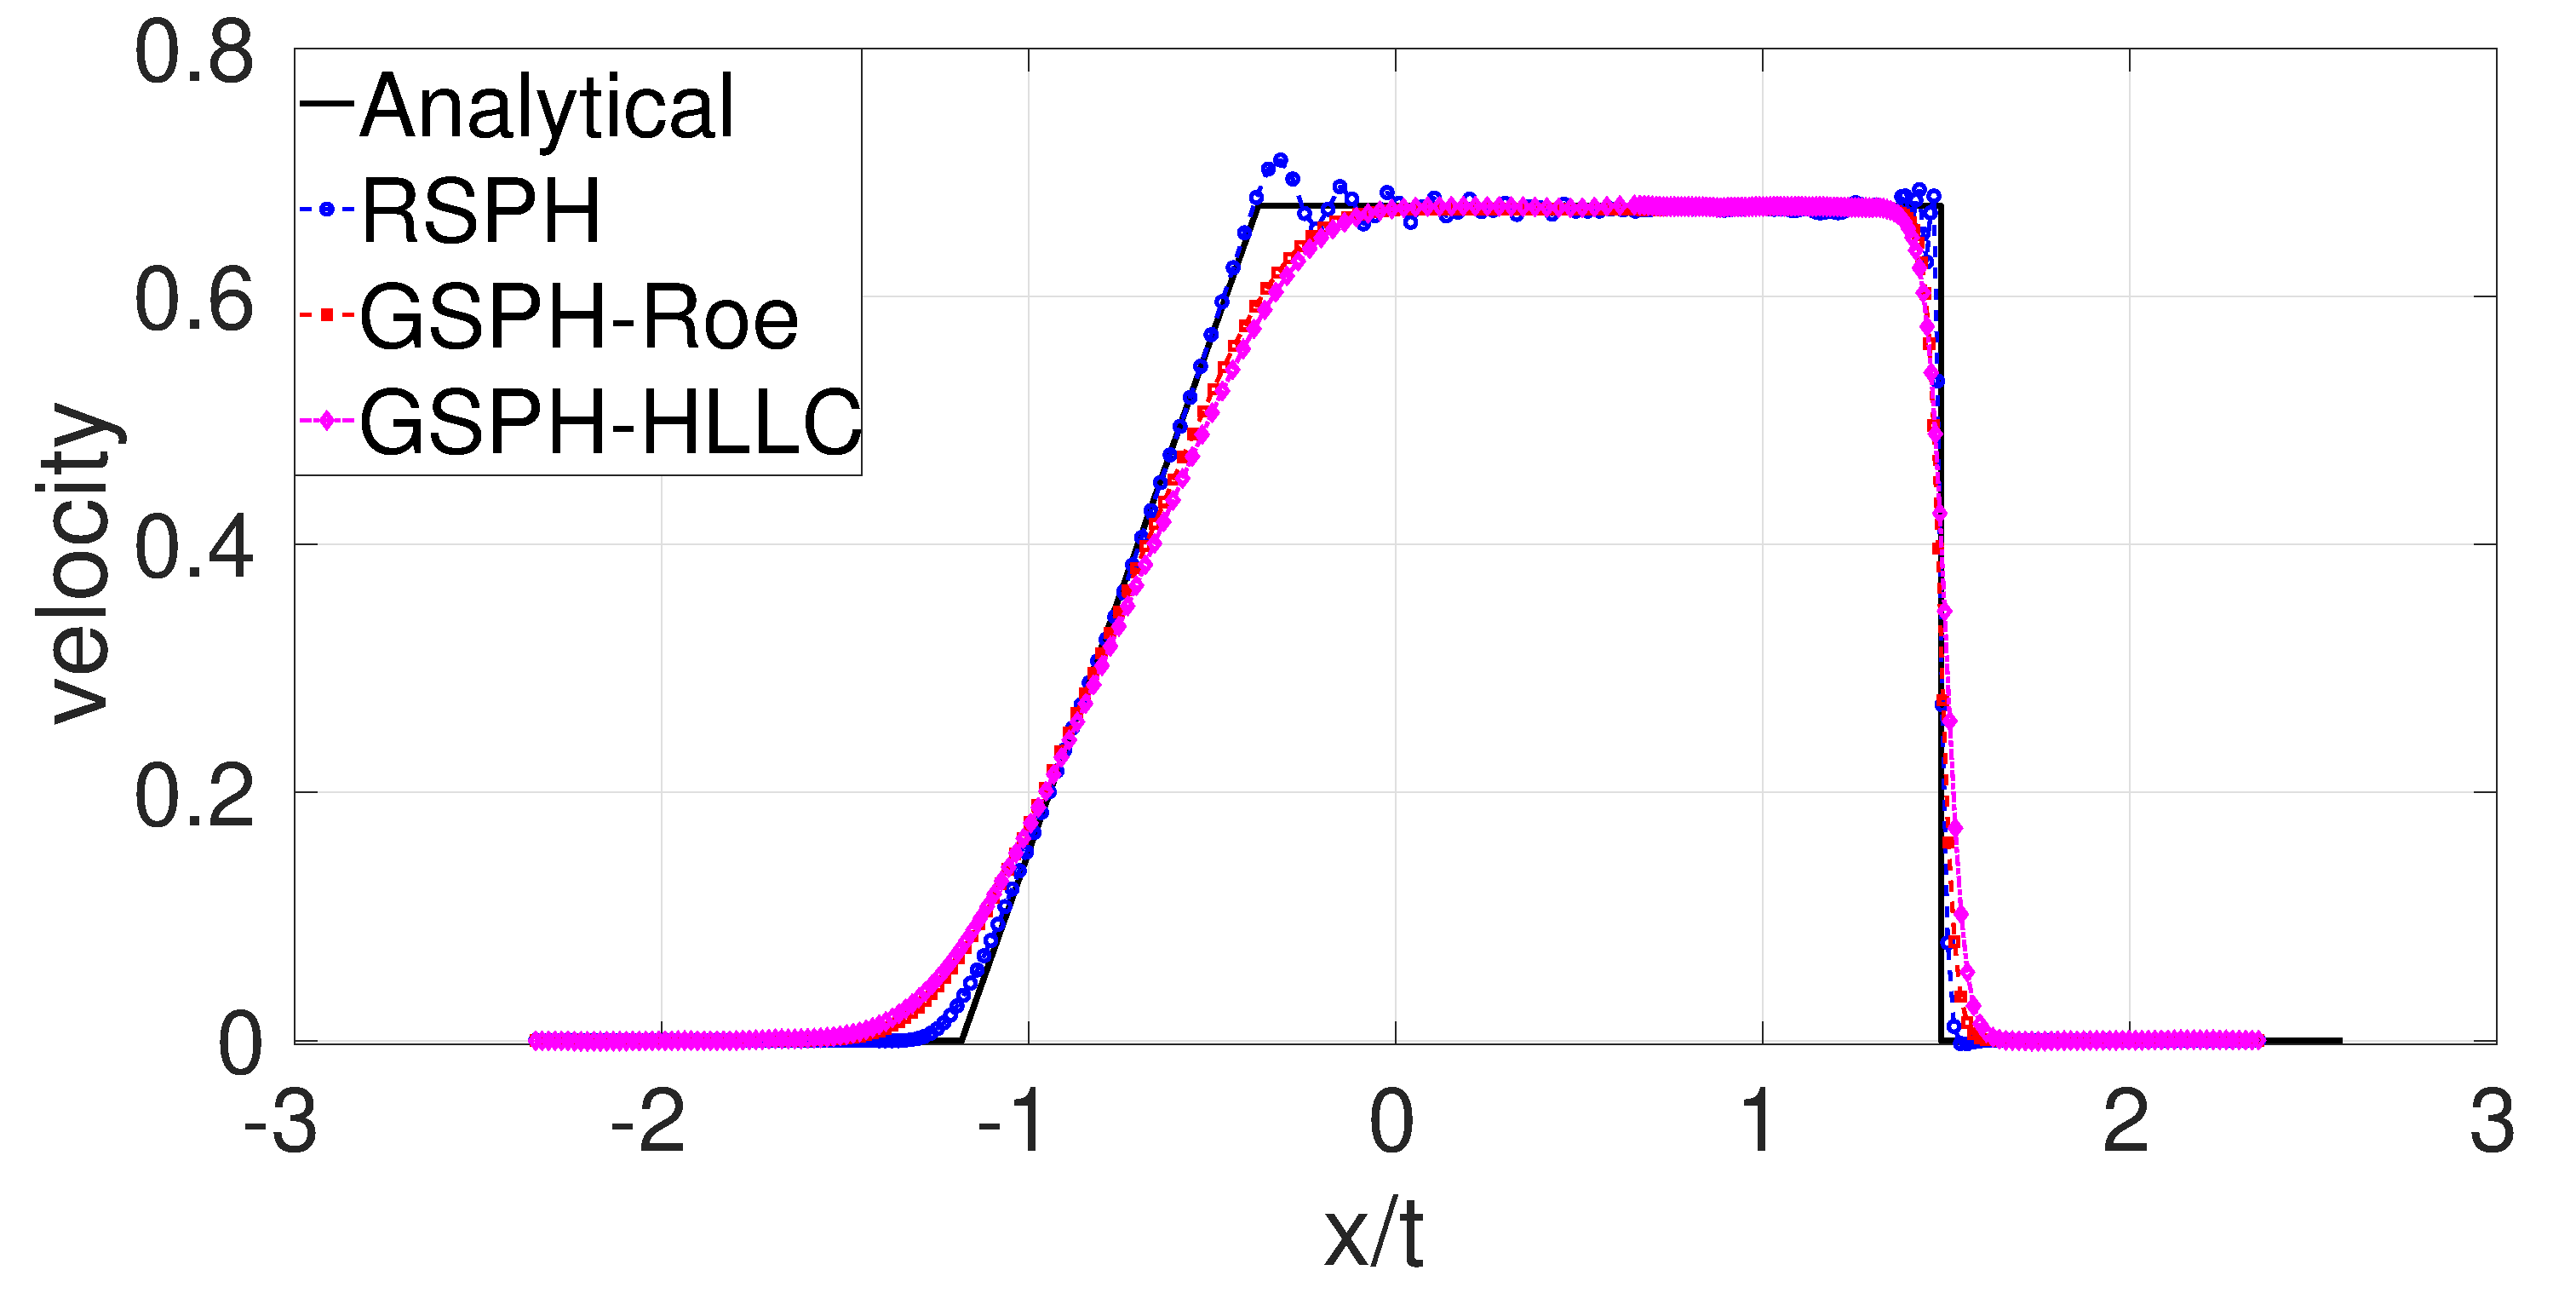
\includegraphics[width=0.99 \textwidth,height=0.6\textwidth]{./Chapter-4/Figures/Sod/RCM-Sod-GSPH-compare-v}
    \end{minipage}%
    \\
    \begin{minipage}{.495\textwidth}
        \centering
        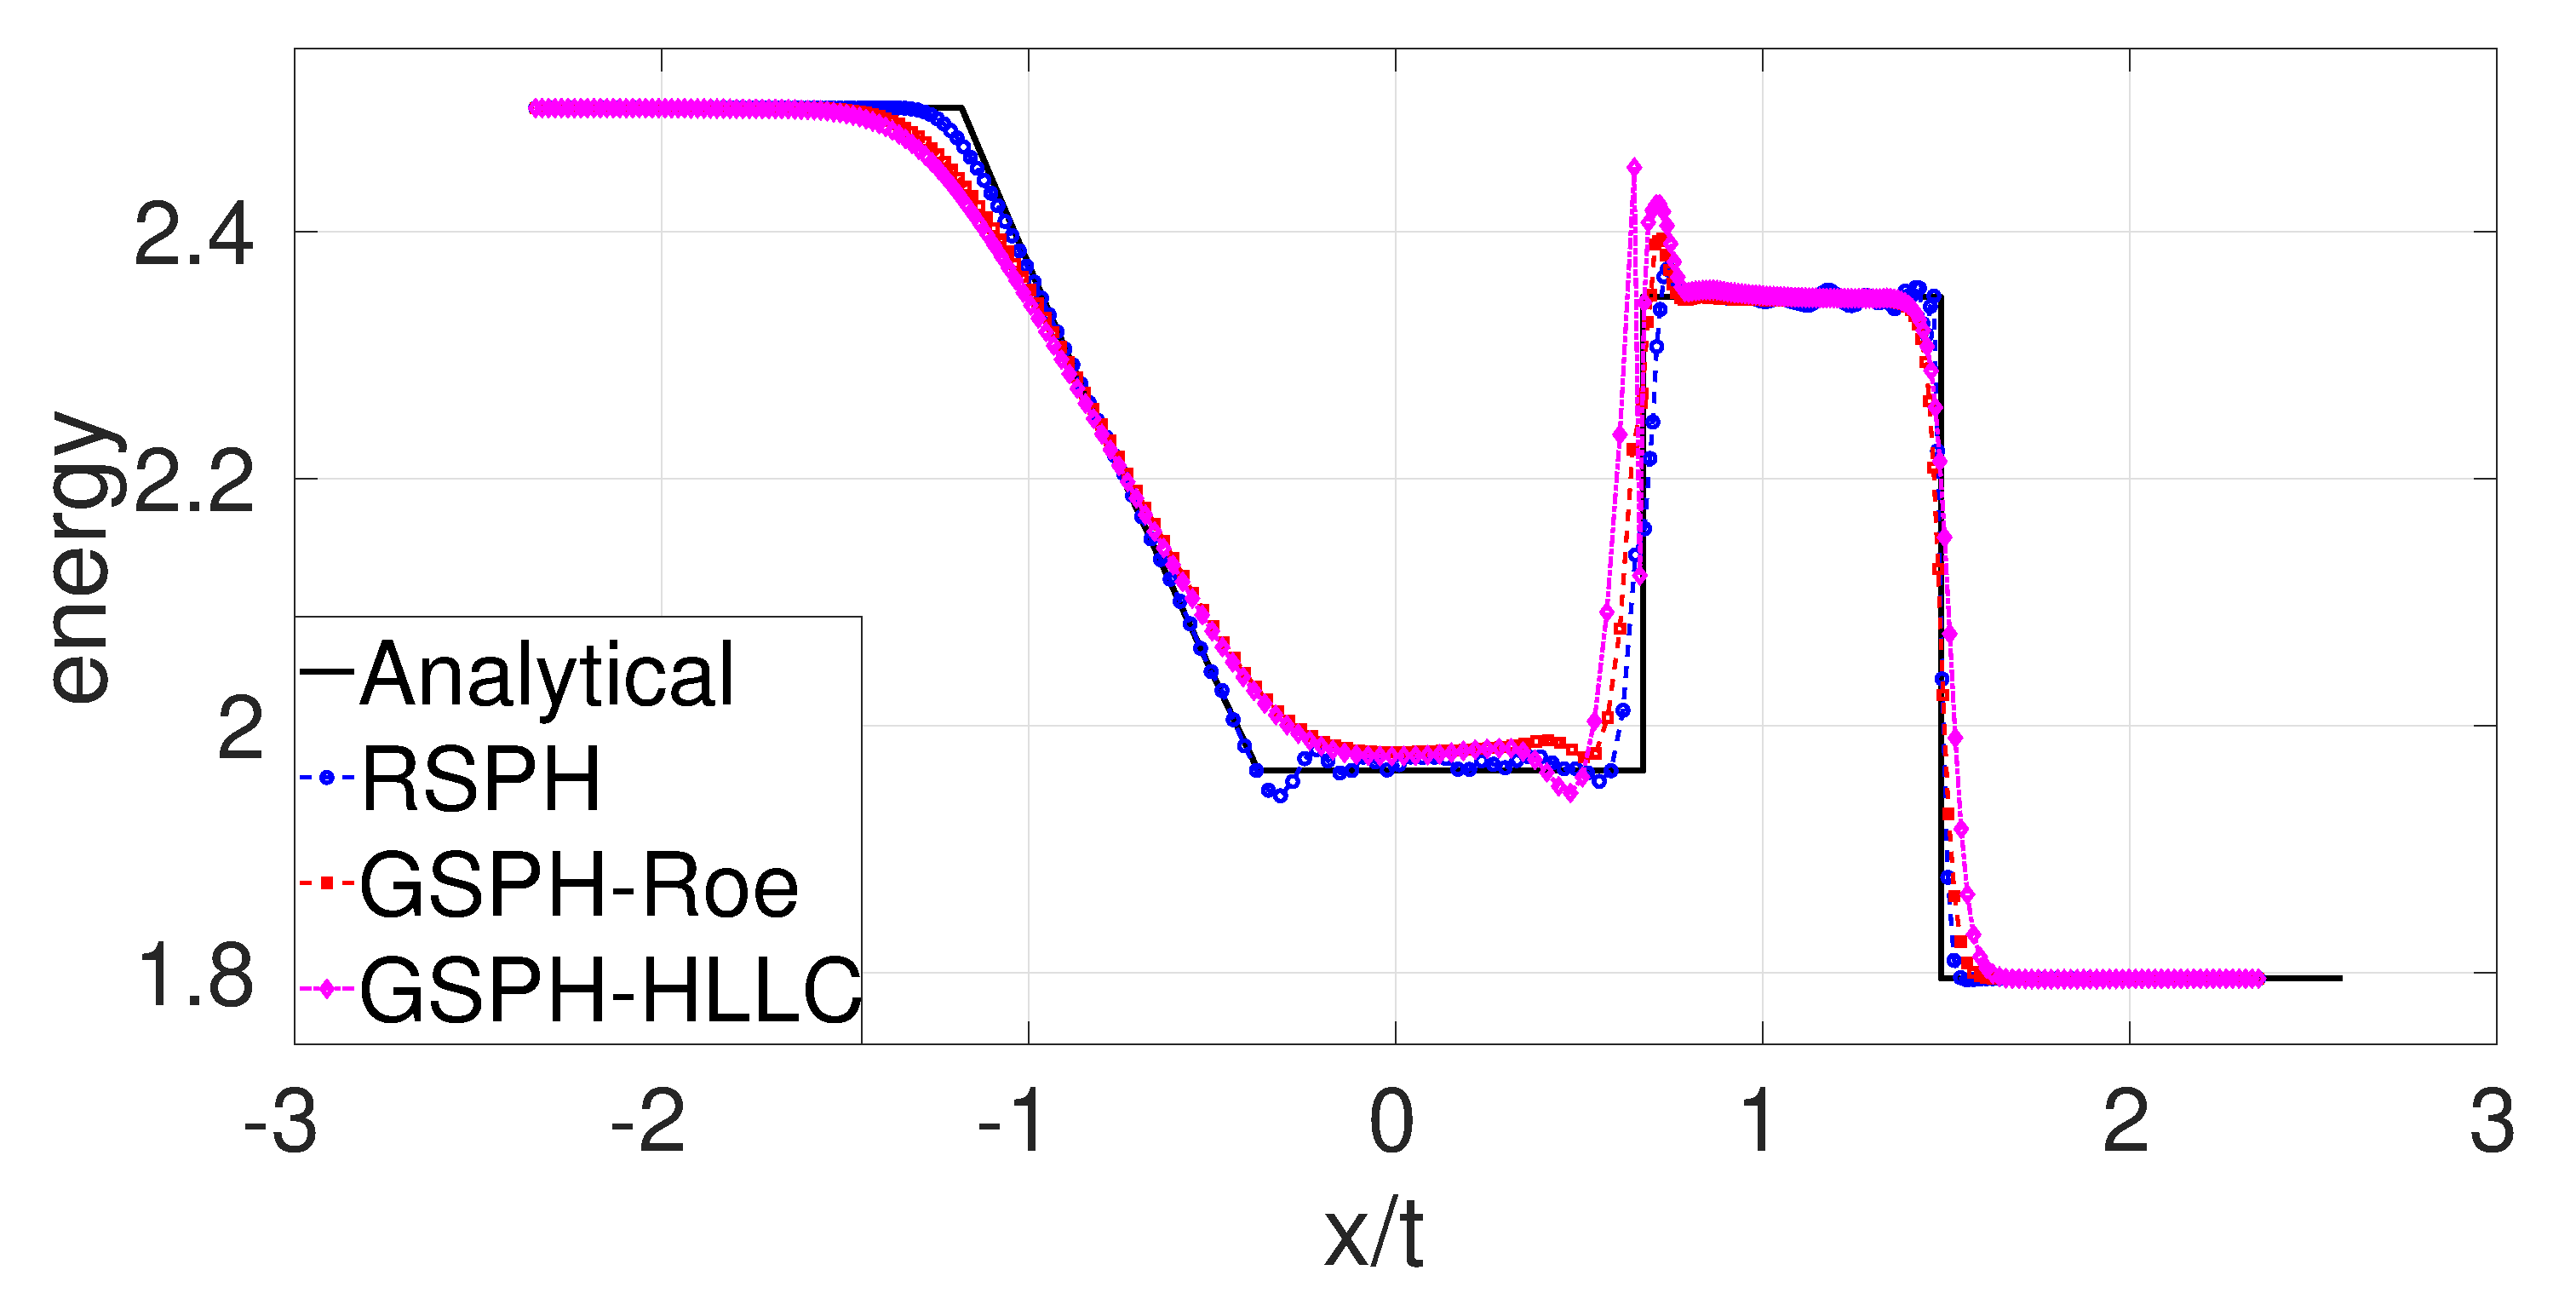
\includegraphics[width=0.99 \textwidth,height=0.6\textwidth]{./Chapter-4/Figures/Sod/RCM-Sod-GSPH-compare-e}
    \end{minipage}%
    \begin{minipage}{.495 \textwidth}
        \centering
        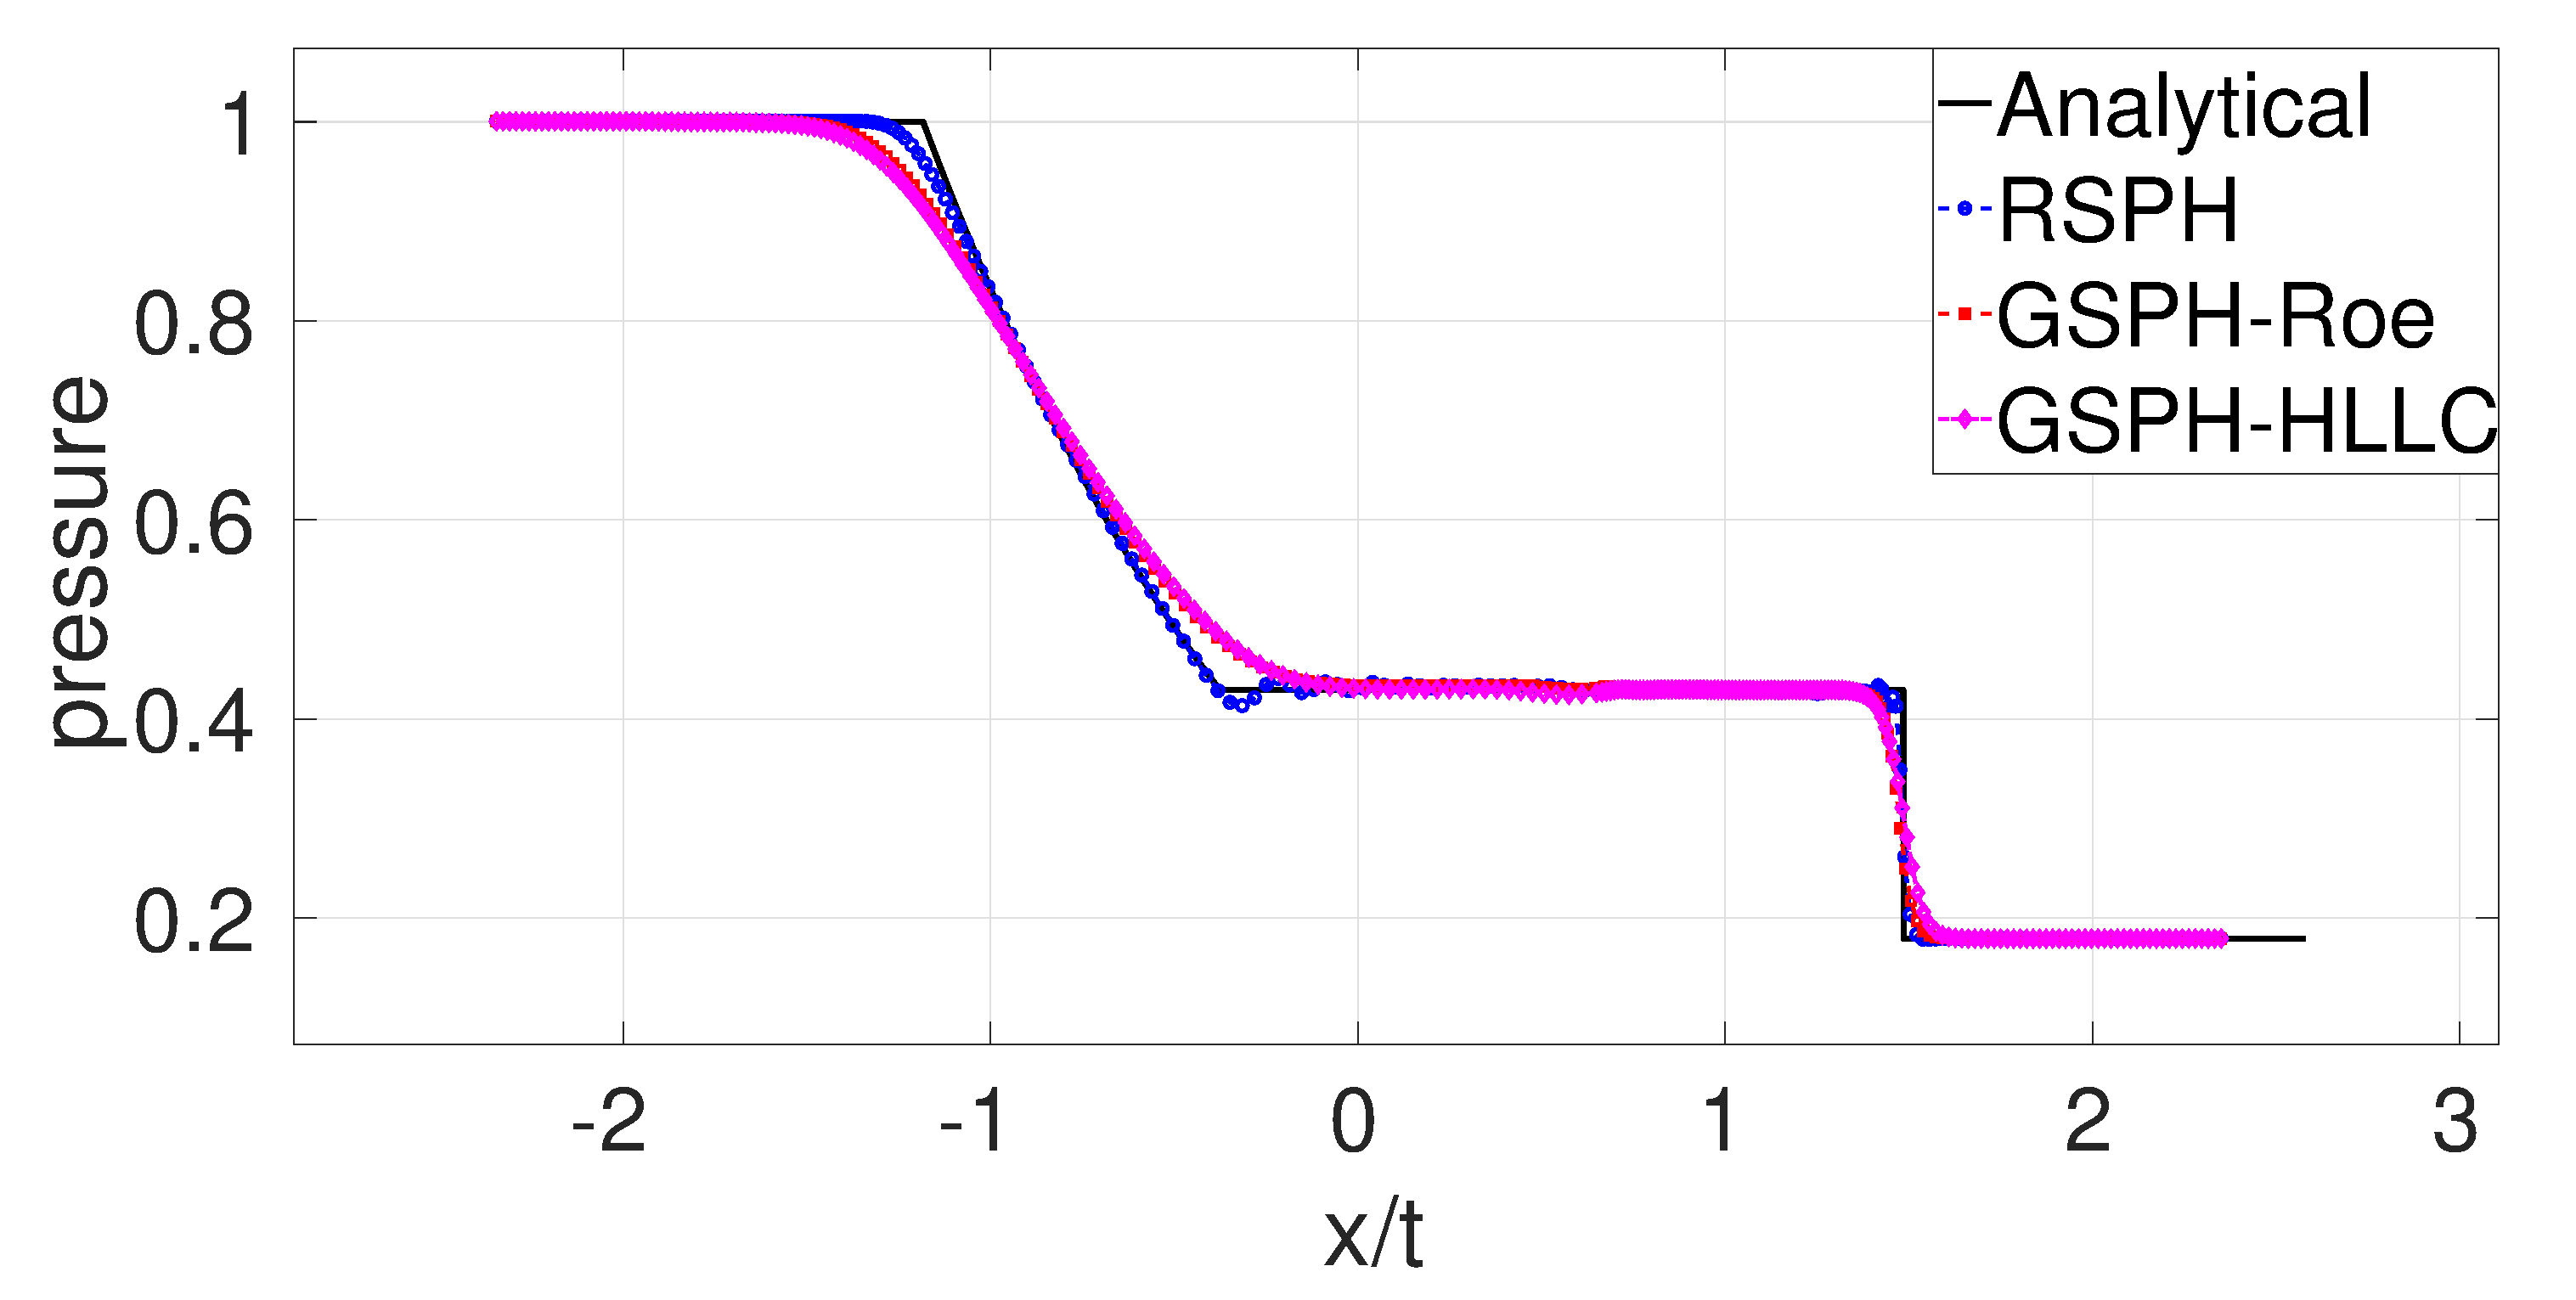
\includegraphics[width=0.99 \textwidth,height=0.6\textwidth]{./Chapter-4/Figures/Sod/RCM-Sod-GSPH-compare-p}
    \end{minipage}% 
    \\
    \begin{minipage}{.495\textwidth}
        \centering
        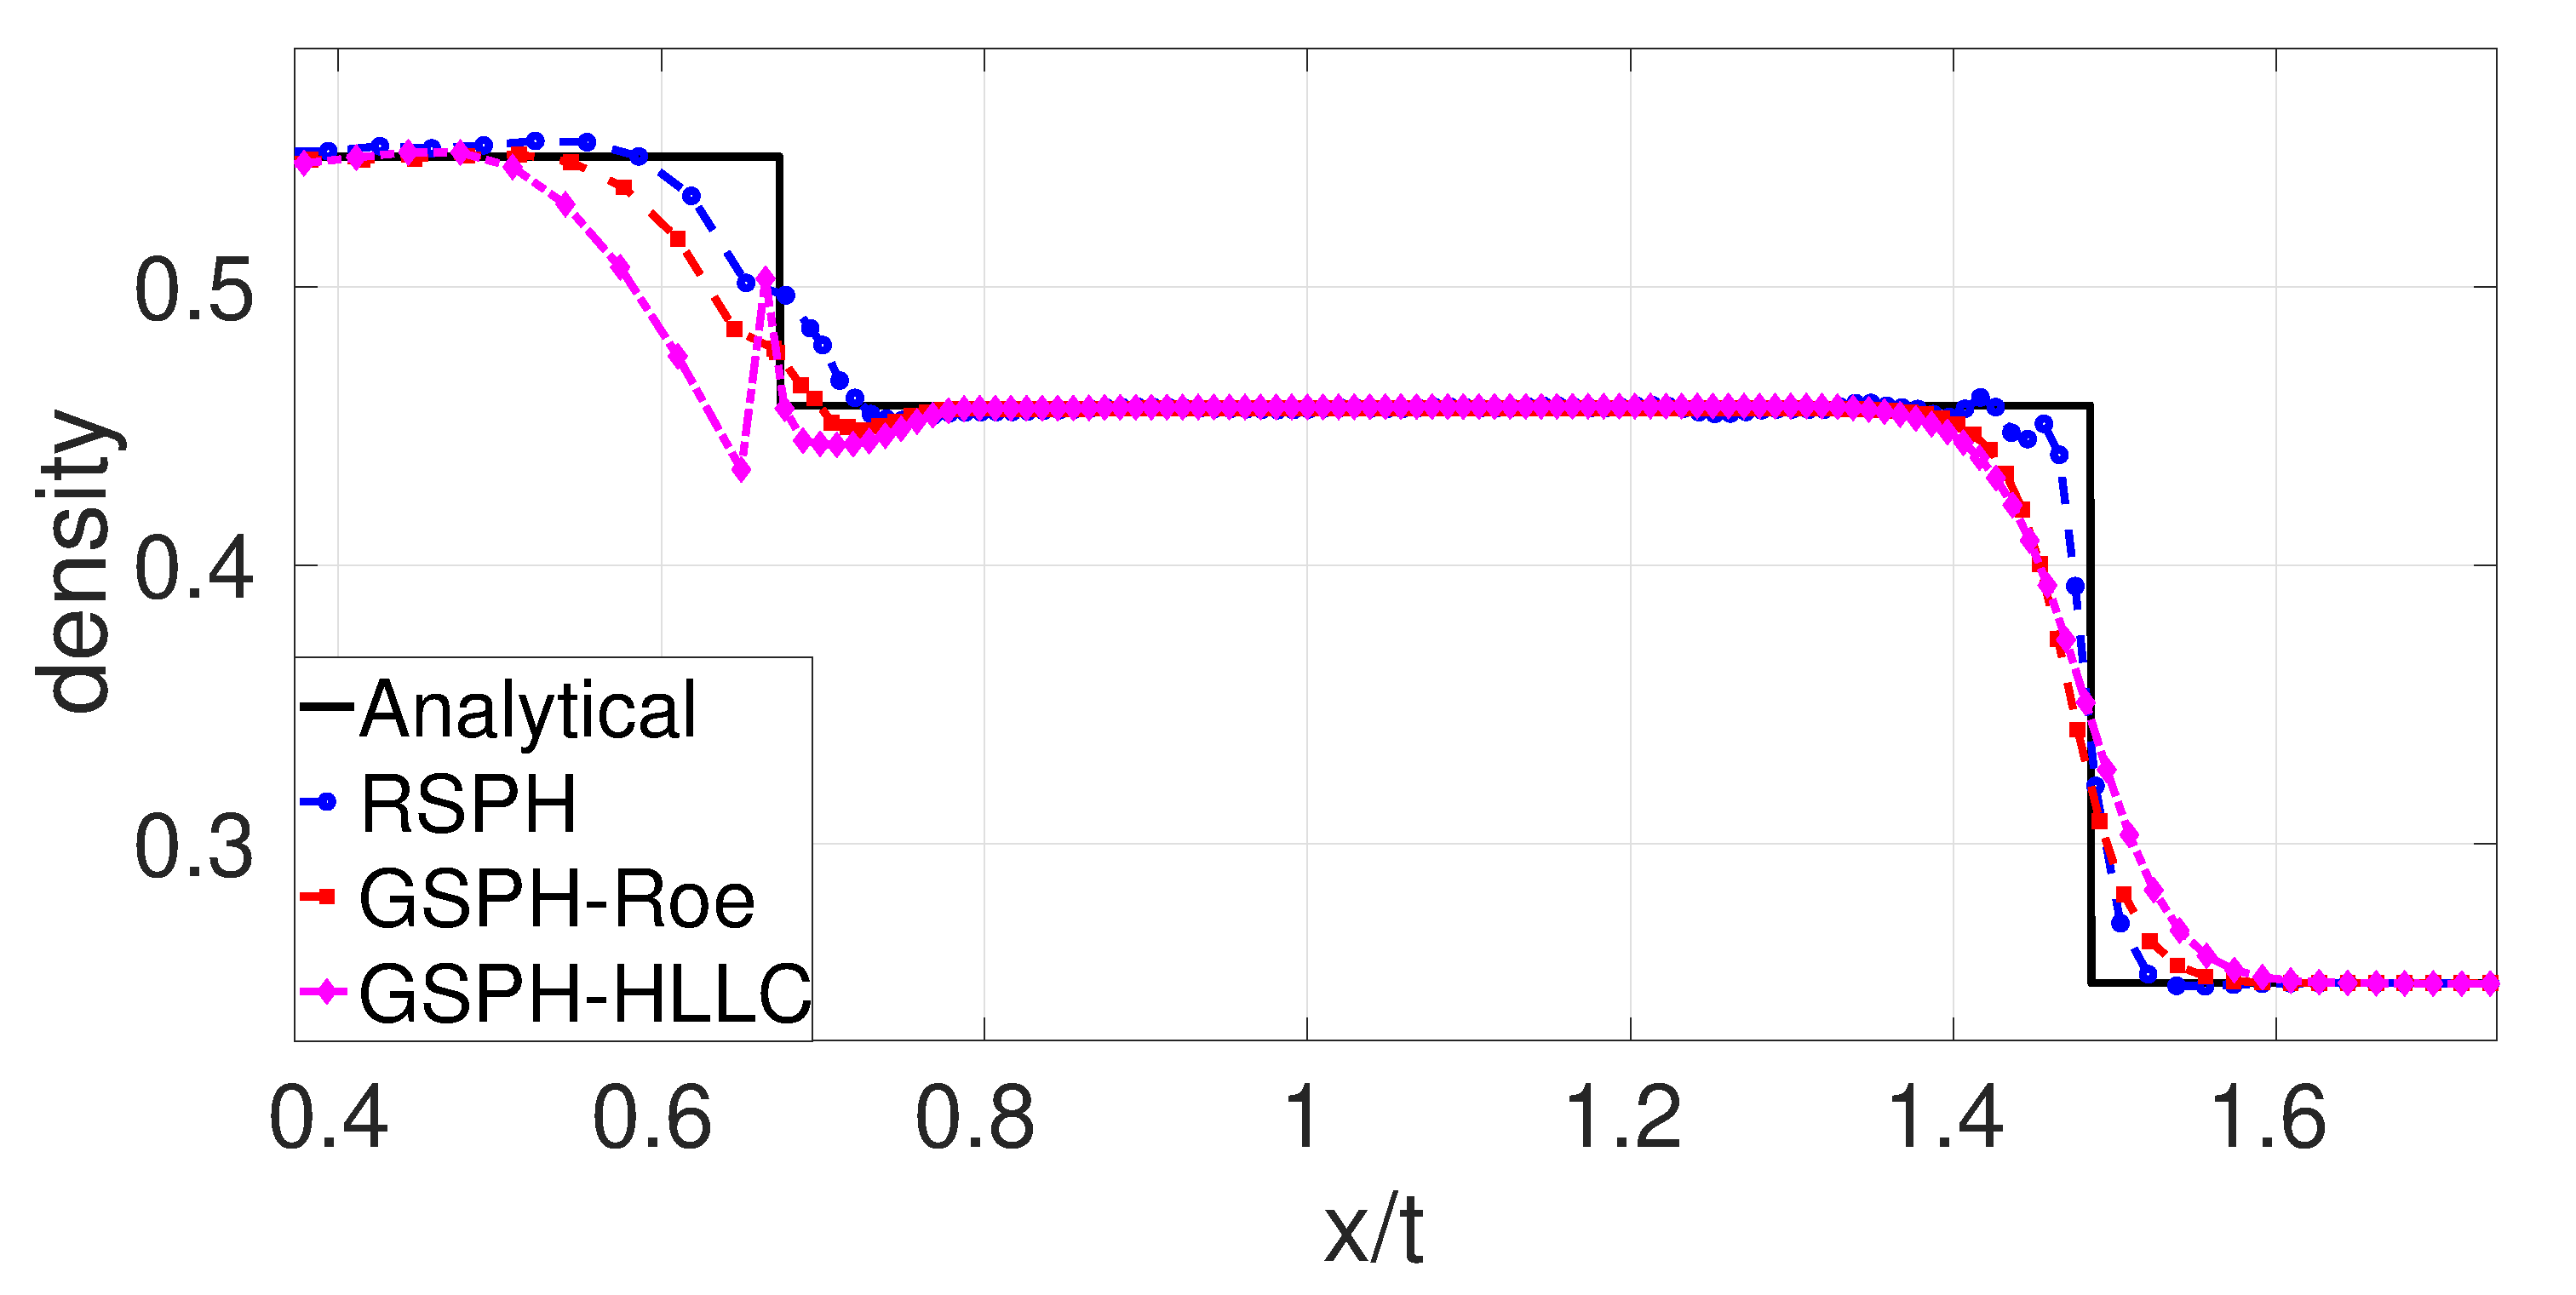
\includegraphics[width=0.99 \textwidth,height=0.6\textwidth]{./Chapter-4/Figures/Sod/RCM-Sod-GSPH-compare-rho-zoom}
    \end{minipage}%
    \begin{minipage}{.495 \textwidth}
        \centering
        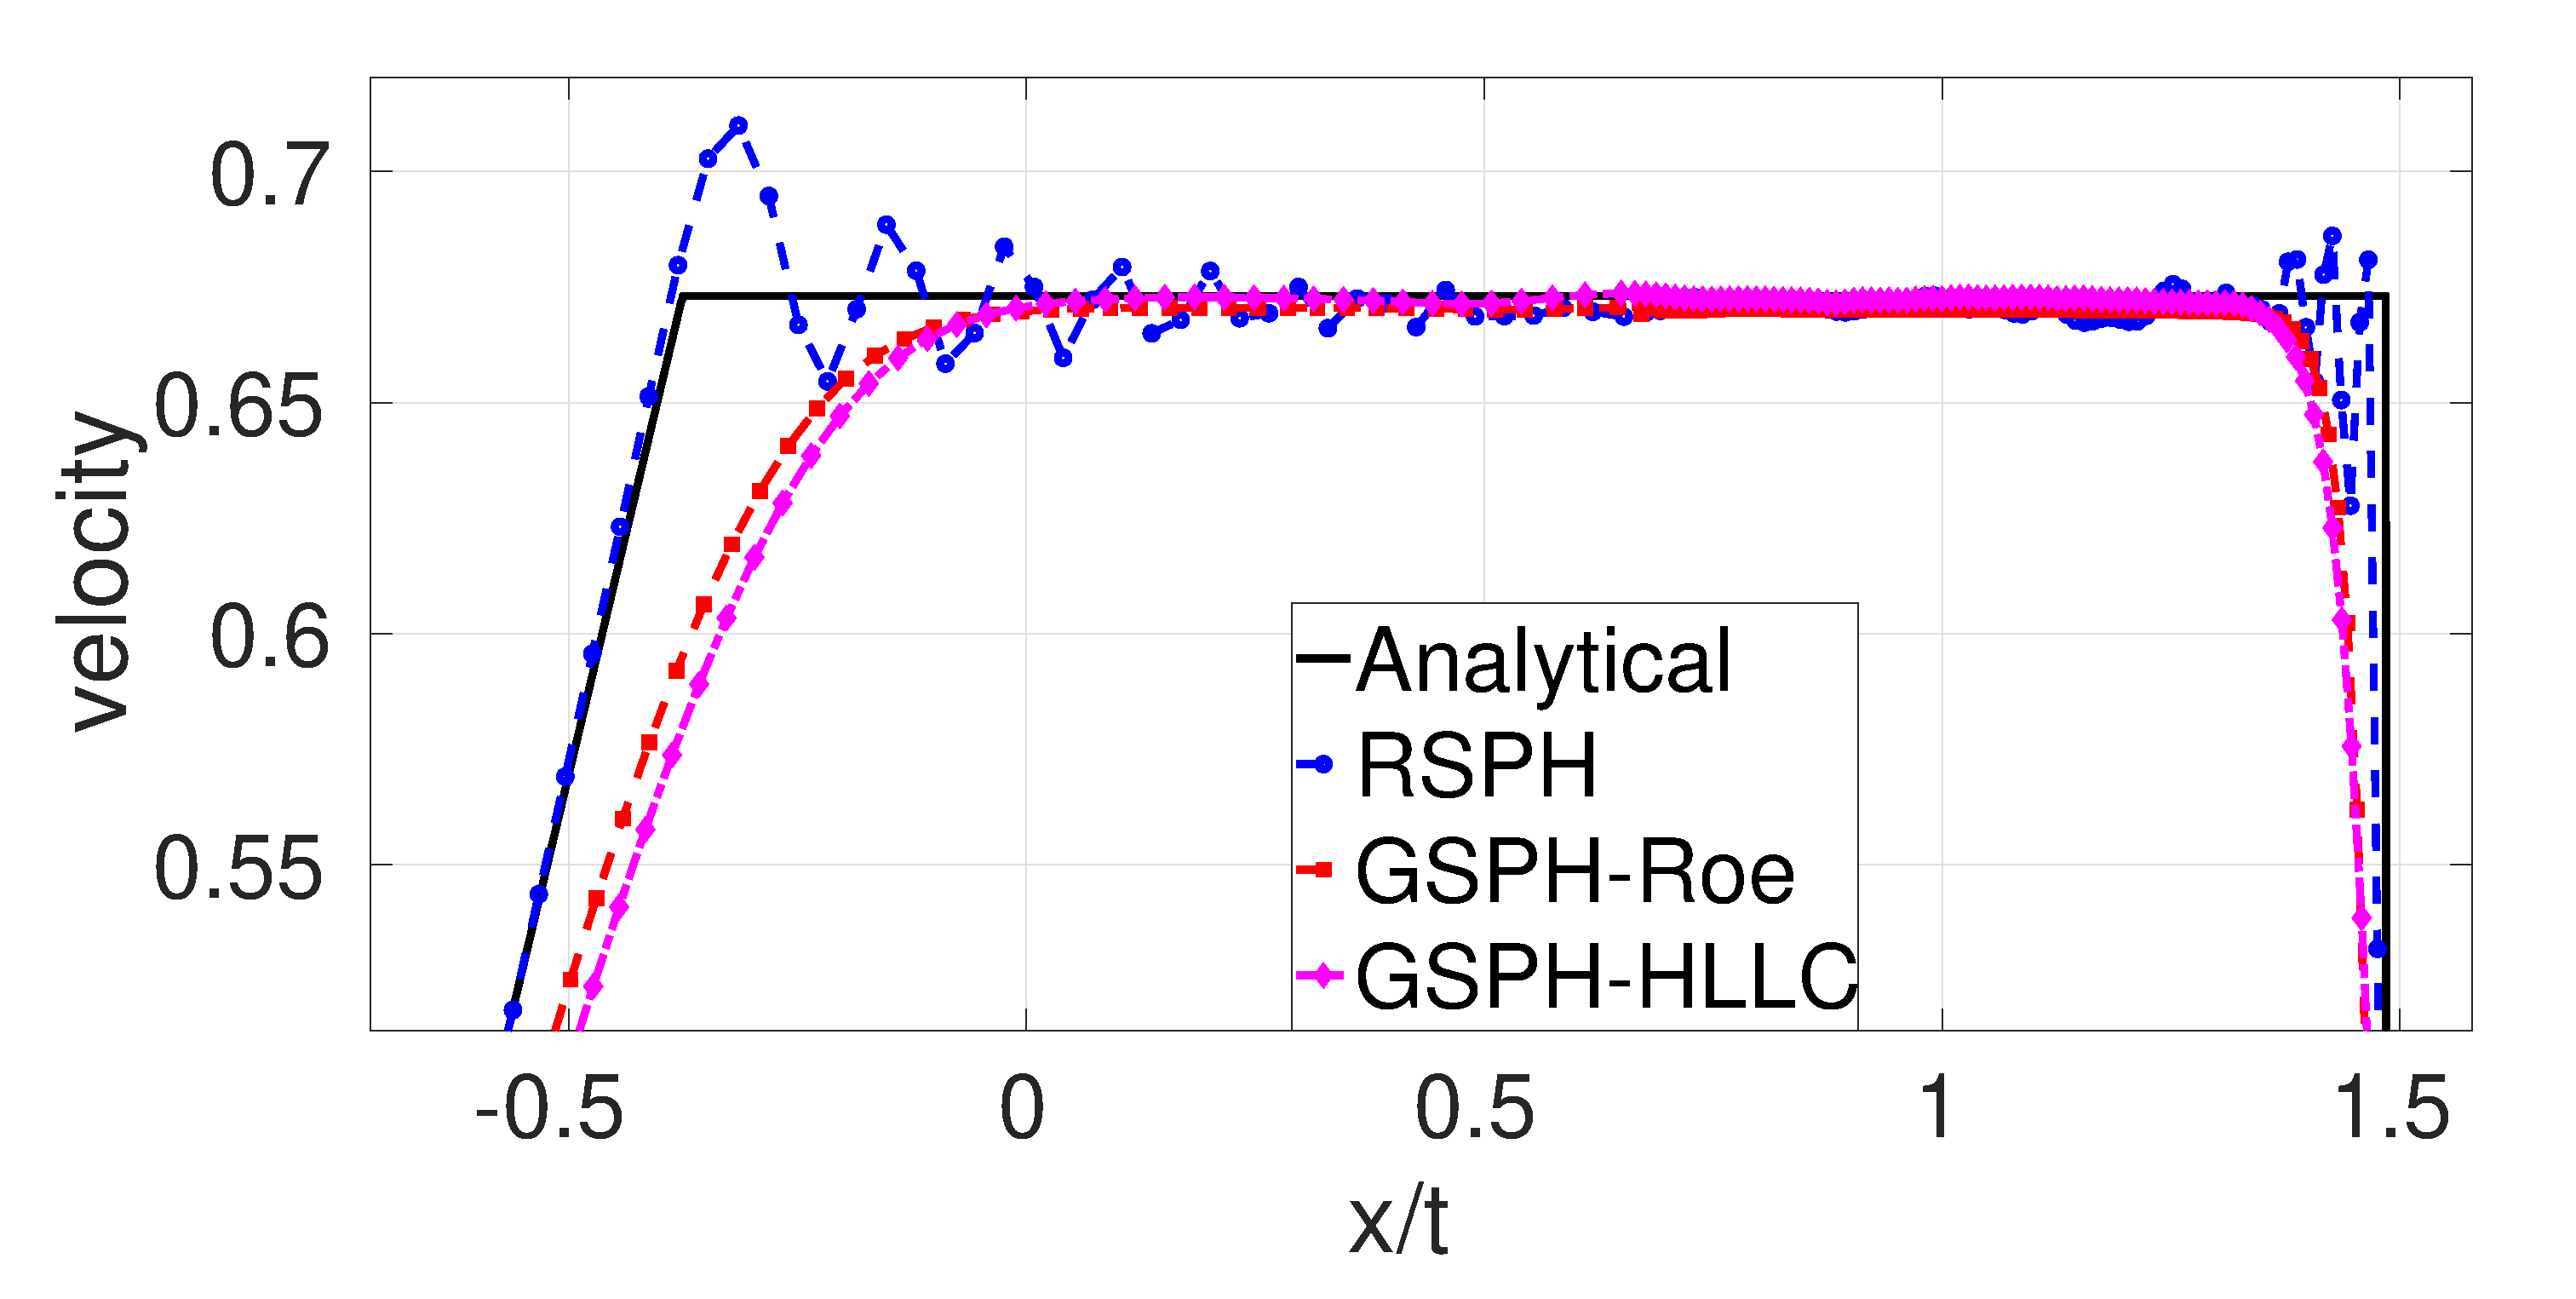
\includegraphics[width=0.99 \textwidth,height=0.6\textwidth]{./Chapter-4/Figures/Sod/RCM-Sod-GSPH-compare-v-zoom}
    \end{minipage}% 
       \\
    \begin{minipage}{.495 \textwidth}
        \centering
        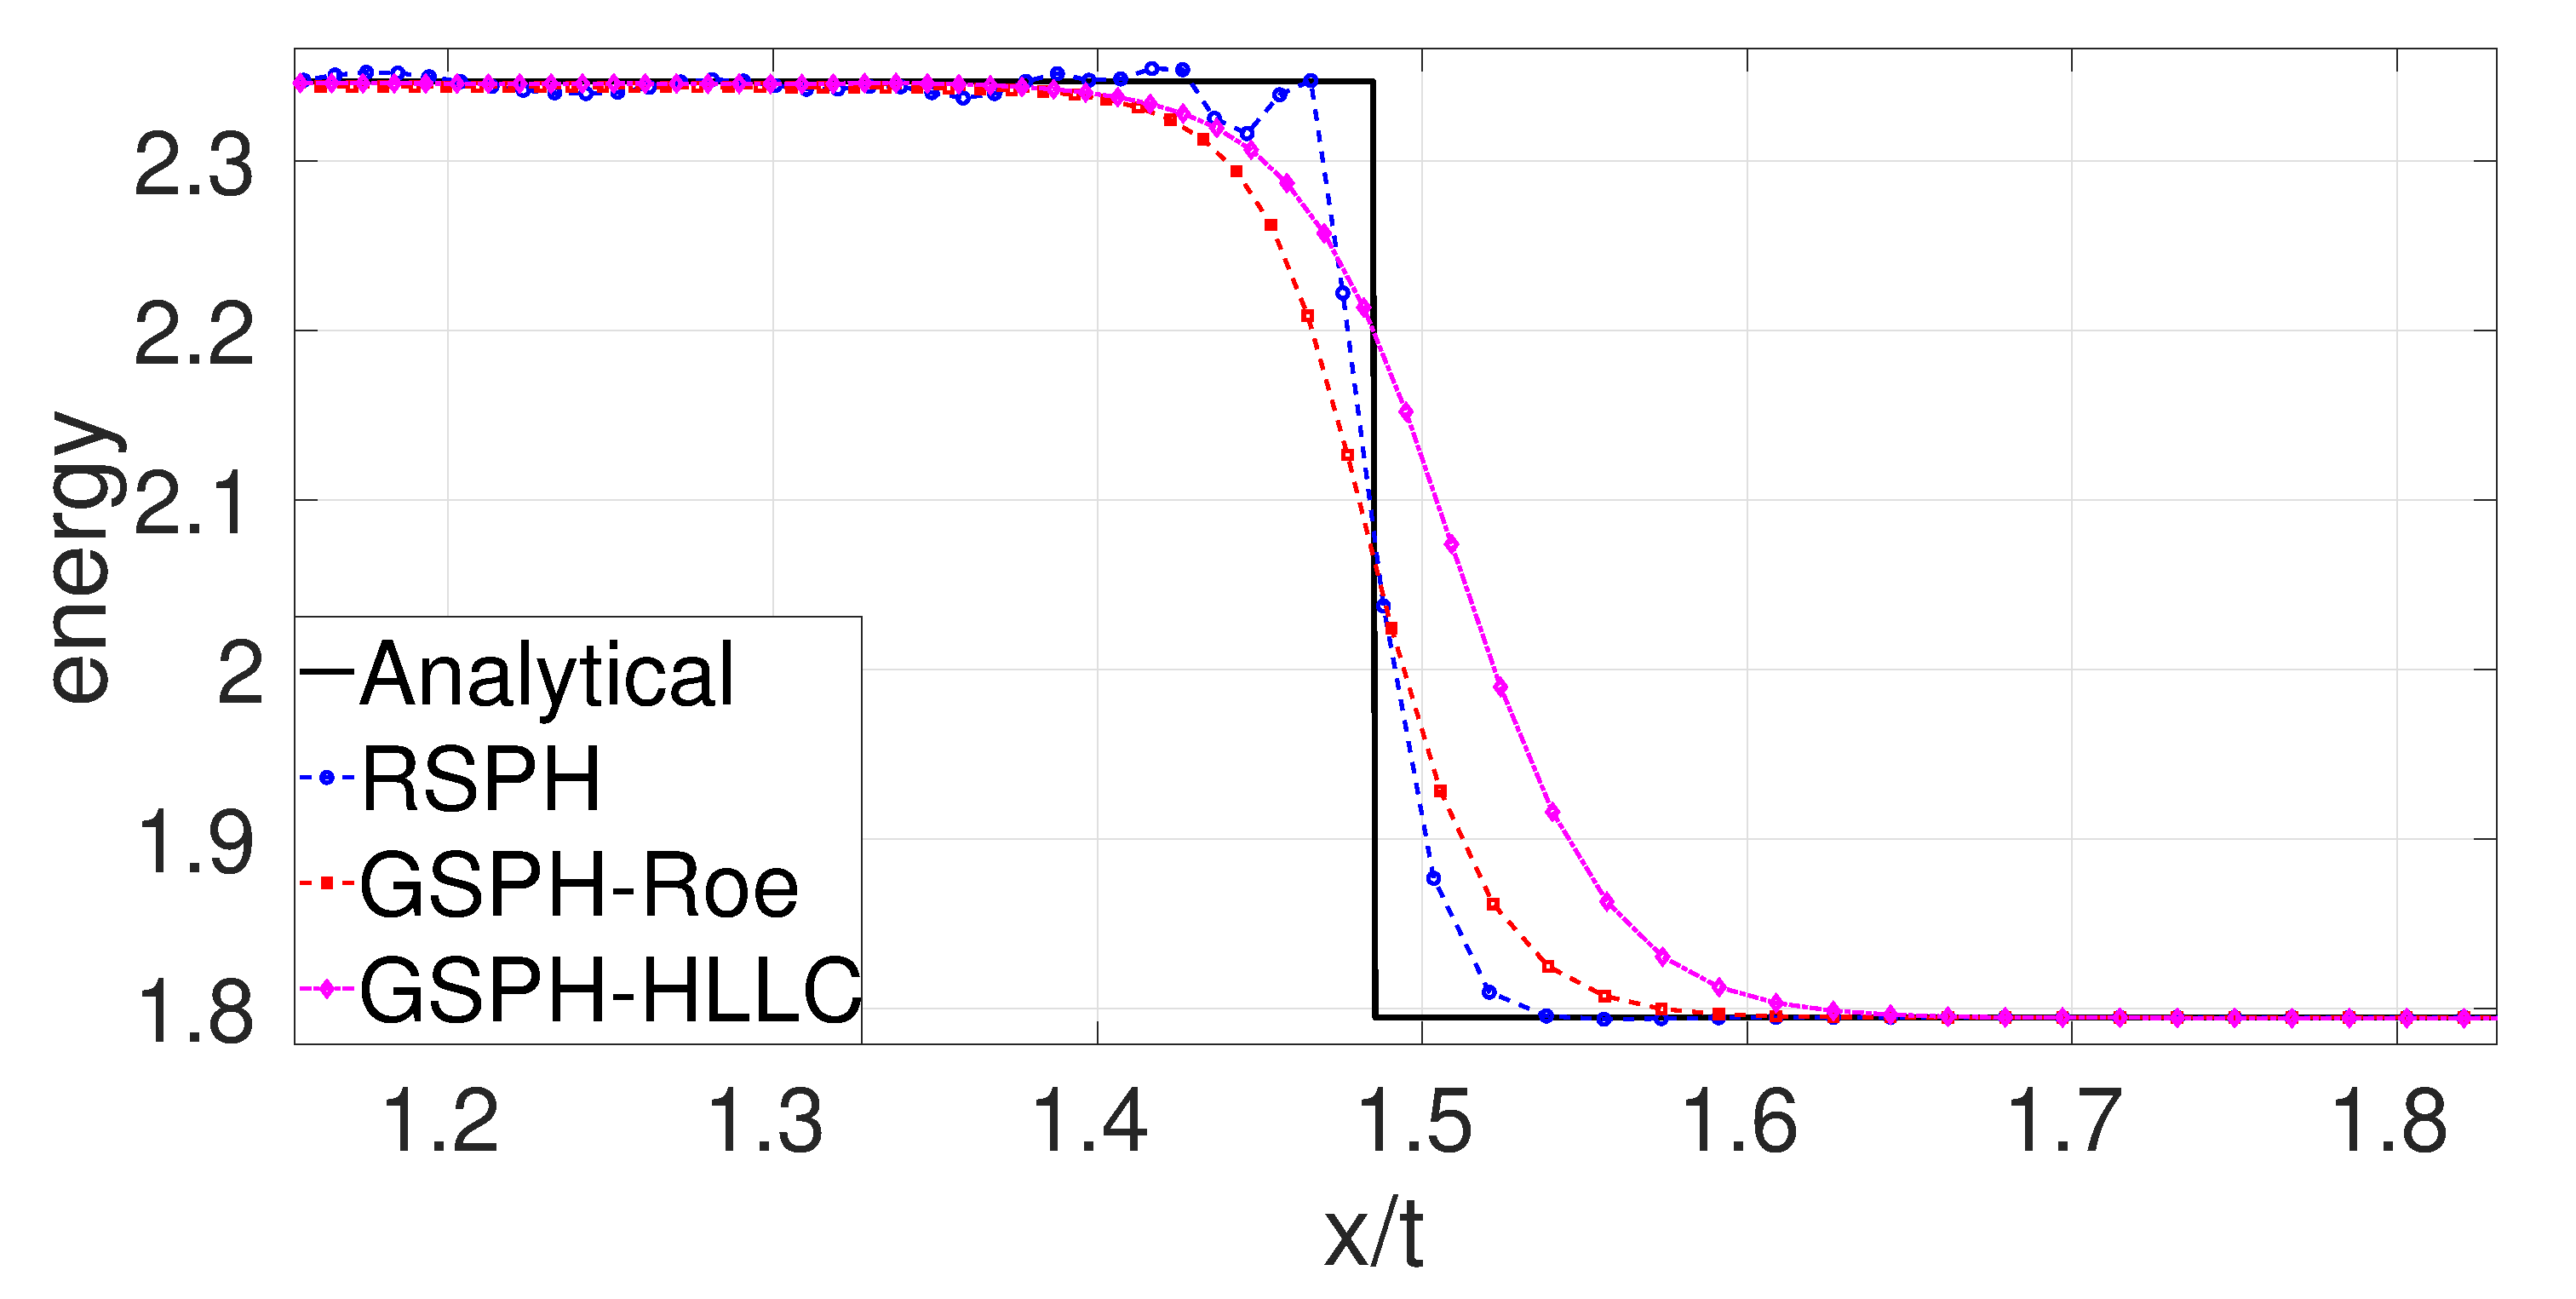
\includegraphics[width=0.99 \textwidth,height=0.6\textwidth]{./Chapter-4/Figures/Sod/RCM-Sod-GSPH-compare-e-zoom}
    \end{minipage}% 
    \begin{minipage}{.495\textwidth}
        \centering
        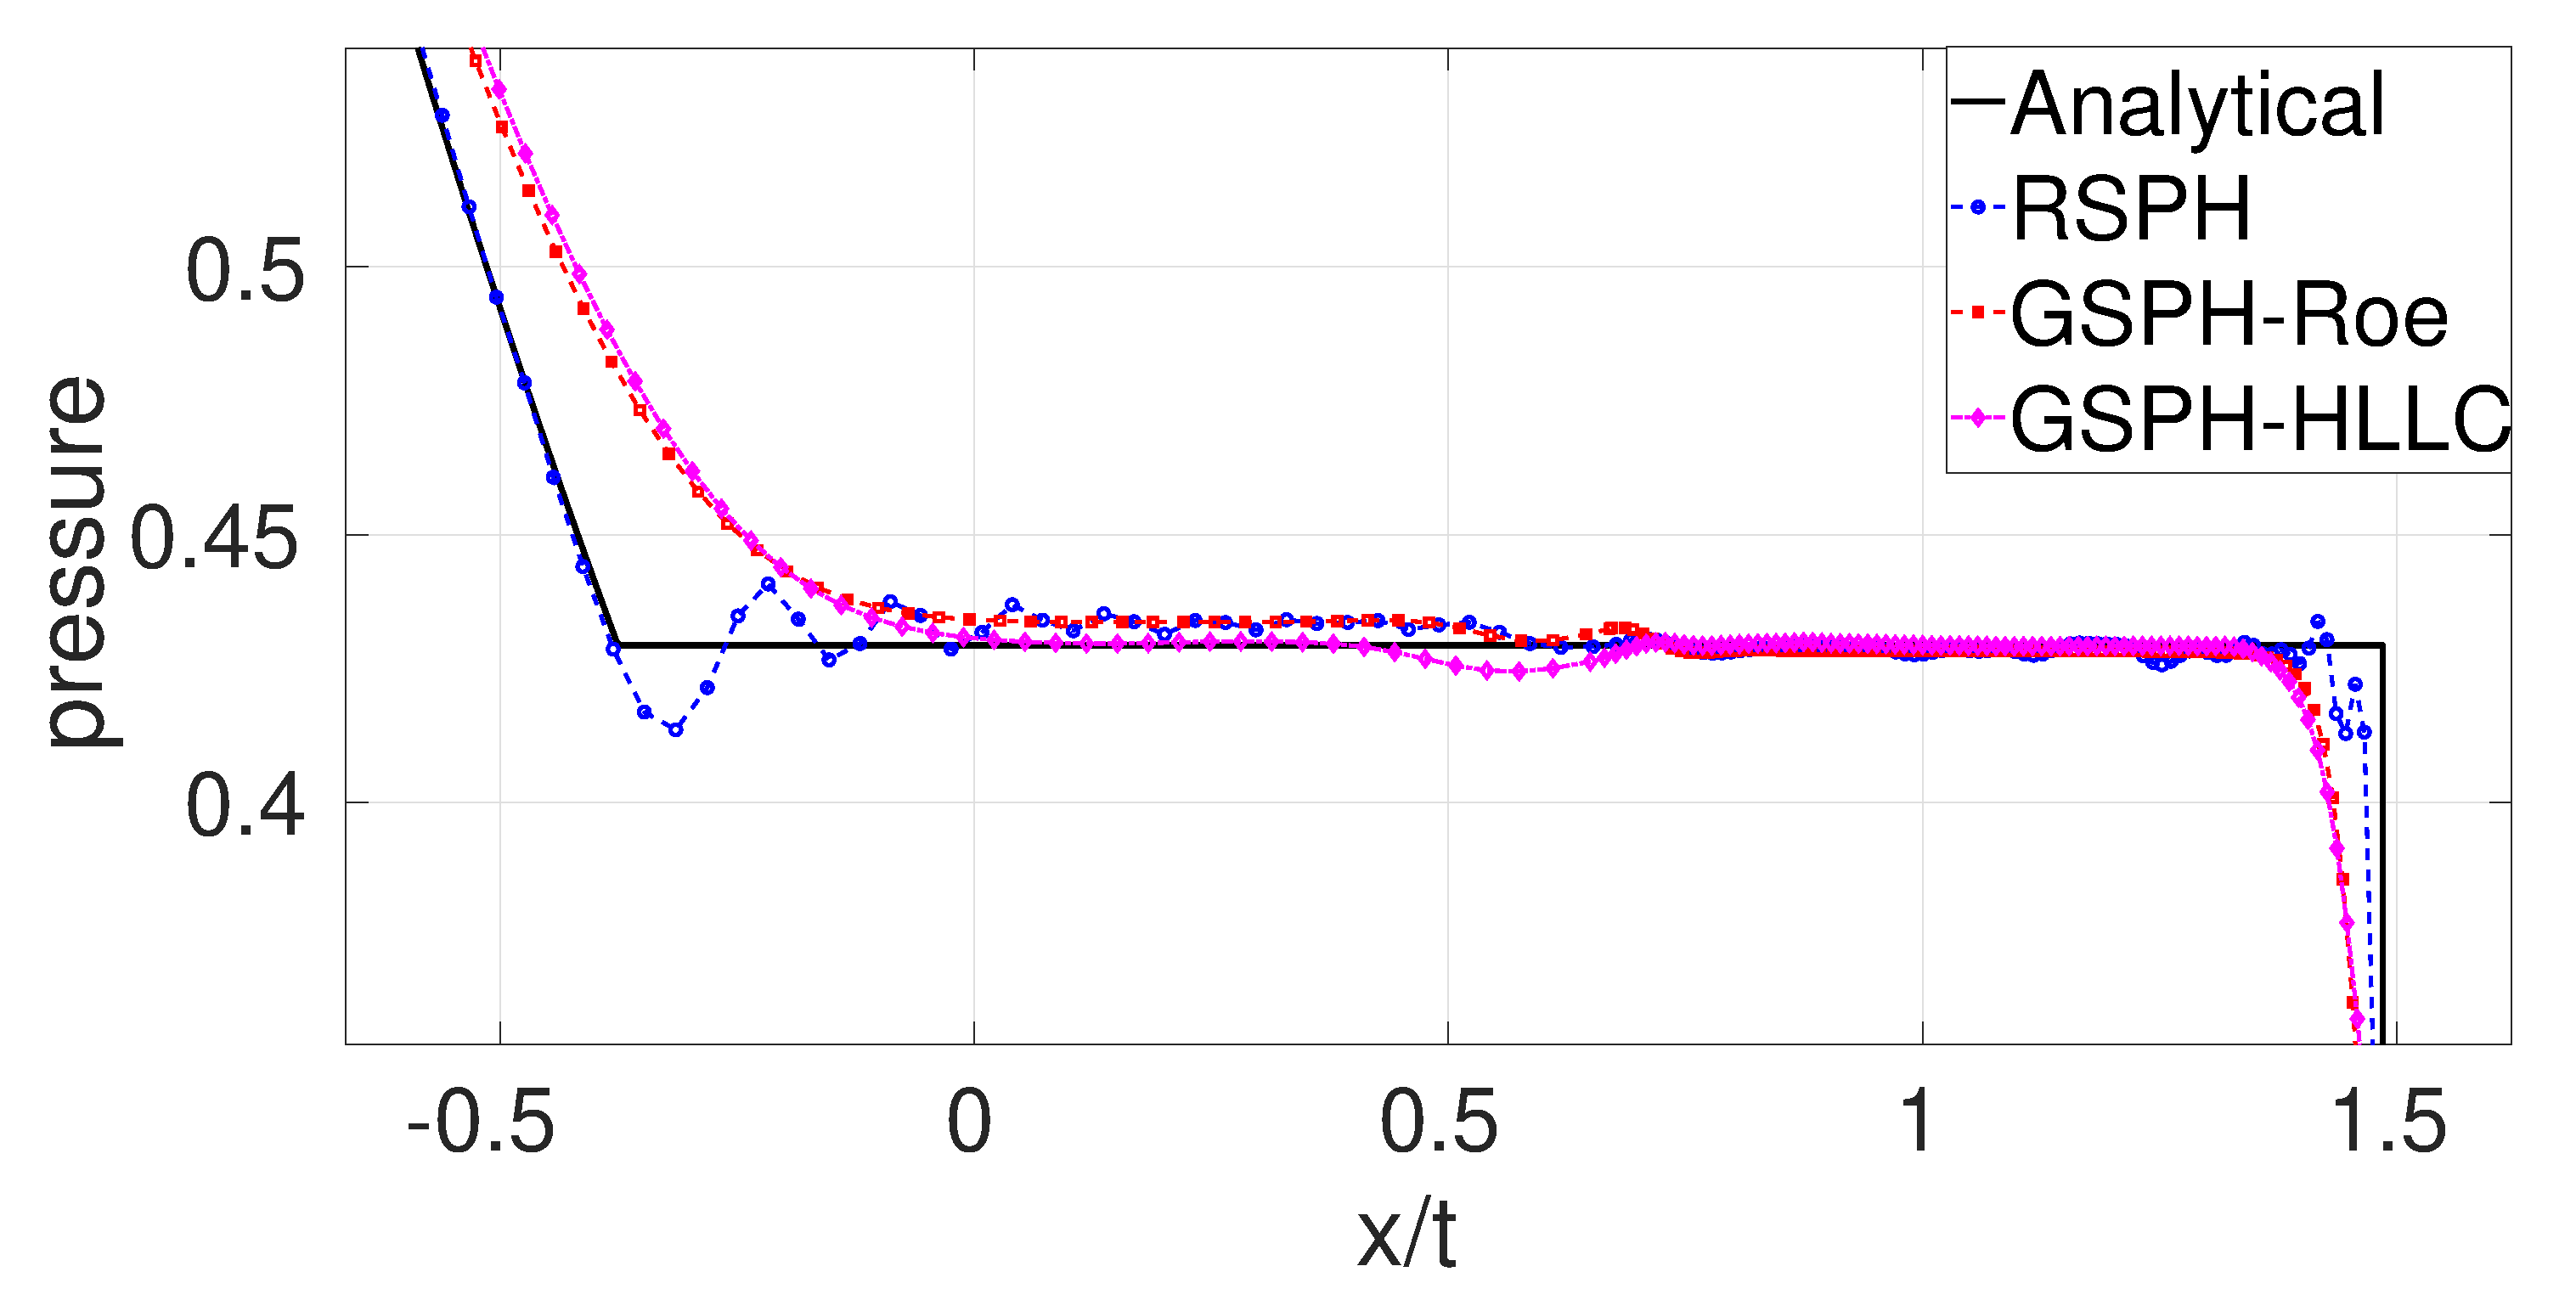
\includegraphics[width=0.99 \textwidth,height=0.6\textwidth]{./Chapter-4/Figures/Sod/RCM-Sod-GSPH-compare-p-zoom}
    \end{minipage}%    
    \caption{Comparison of RSPH with GSPH using Roe Riemann solver and HLLC Riemann solver. The last four plots are zoomed views. Zoomed view of density and specific internal energy show that GSPH smears the discontinuity at shock much more than RSPH. Zoomed view of velocity shows that fluctuation in GSPH is completely suppressed, which implies that numerical dissipation introduced in GSPH is at least around the same amount as SPH with $\alpha=1.0$. This is consistent with information implied by zoomed view of density and specific internal energy. The last zoomed view shows that both RSPH and GSPH can get rid of pressure ``wiggle" around the contact discontinuity.}
    \label{fig:RCM-Sod-GSPH}
\end{figure}

Zoomed views in Fig. \ref{fig:RCM-Sod-GSPH} compare GSPH and RSPH and demonstrate that RSPH introduces less but sufficient dissipation compared with GSPH. The attractive feature of RCM method in preserving true discontinuity is inherited by RSPH in this 1D shock tube test. With more numerical dissipation, GSPH can completely suppress numerical oscillations. However, the discontinuity at the shock is then more seriously smeared. The excessive amount of dissipation might have other, more undesirable, effects in real implementation. For example, over damping of shearing flow. Compared with SPH, both GSPH and RSPH avoid pressure ``wiggle" around contact discontinuity. Since RSPH shares many commonalities   with Godunov's method, it is not a surprise that RSPH can also suppress the pressure ``wiggle" at contact discontinuity.

\subsection{Accuracy tests}
We use shock tube test to gauge the accuracy of the RSPH scheme.
We examine the errors between simulation results and the analytical solution (the reference solution) as the number of particles is increased. The $L_1$ norm error, defined for a property $f$, is normalized by the number of particles as:
\begin{equation}
L_1= \frac{1}{N_p} \sum_a^{N_p} \vert f_a^{SPH} - f^{REF} (x_a) \vert 
\end{equation}
where the superscript $REF$ represent the reference solution, $SPH$ represents simulation results calculated by different SPH schemes. Fig. \ref{fig:Accuracy-test1} displays the $L_1$ norm errors for the density, velocity and pressure profiles for different SPH schemes.
We observe a rate of convergence of approximately 1 for GSPH and 1.5 for standard SPH and RSPH.
GSPH with an exact Riemann solver has been shown to be approximately second order of accuracy \citep{puri2014comparison} and comparable in accuracy to the standard SPH schemes when using piece wise linear construction. As for GSPH using approximate Riemann solver, \citet{puri2014approximate} reported second order accuracy for HLLC and Roe Riemann solvers adopting piece wise linear Riemann problem construction. In addition, they adopted a test problem without discontinuity in the solution. Presence of discontinuities, such as shock, in the test problem might lower the rate of convergence. Since both RSPH and GSPH tests in this chapter adopt piece wise constant construction of Riemann problem. We conclude that RSPH shows higher order of accuracy than GSPH when using the same Riemann problem construction. Compared with SPH, RSPH shows almost the same order of accuracy and level of error.  
\begin{figure}
    \centering
    \begin{minipage}{.332\textwidth}
        \centering
        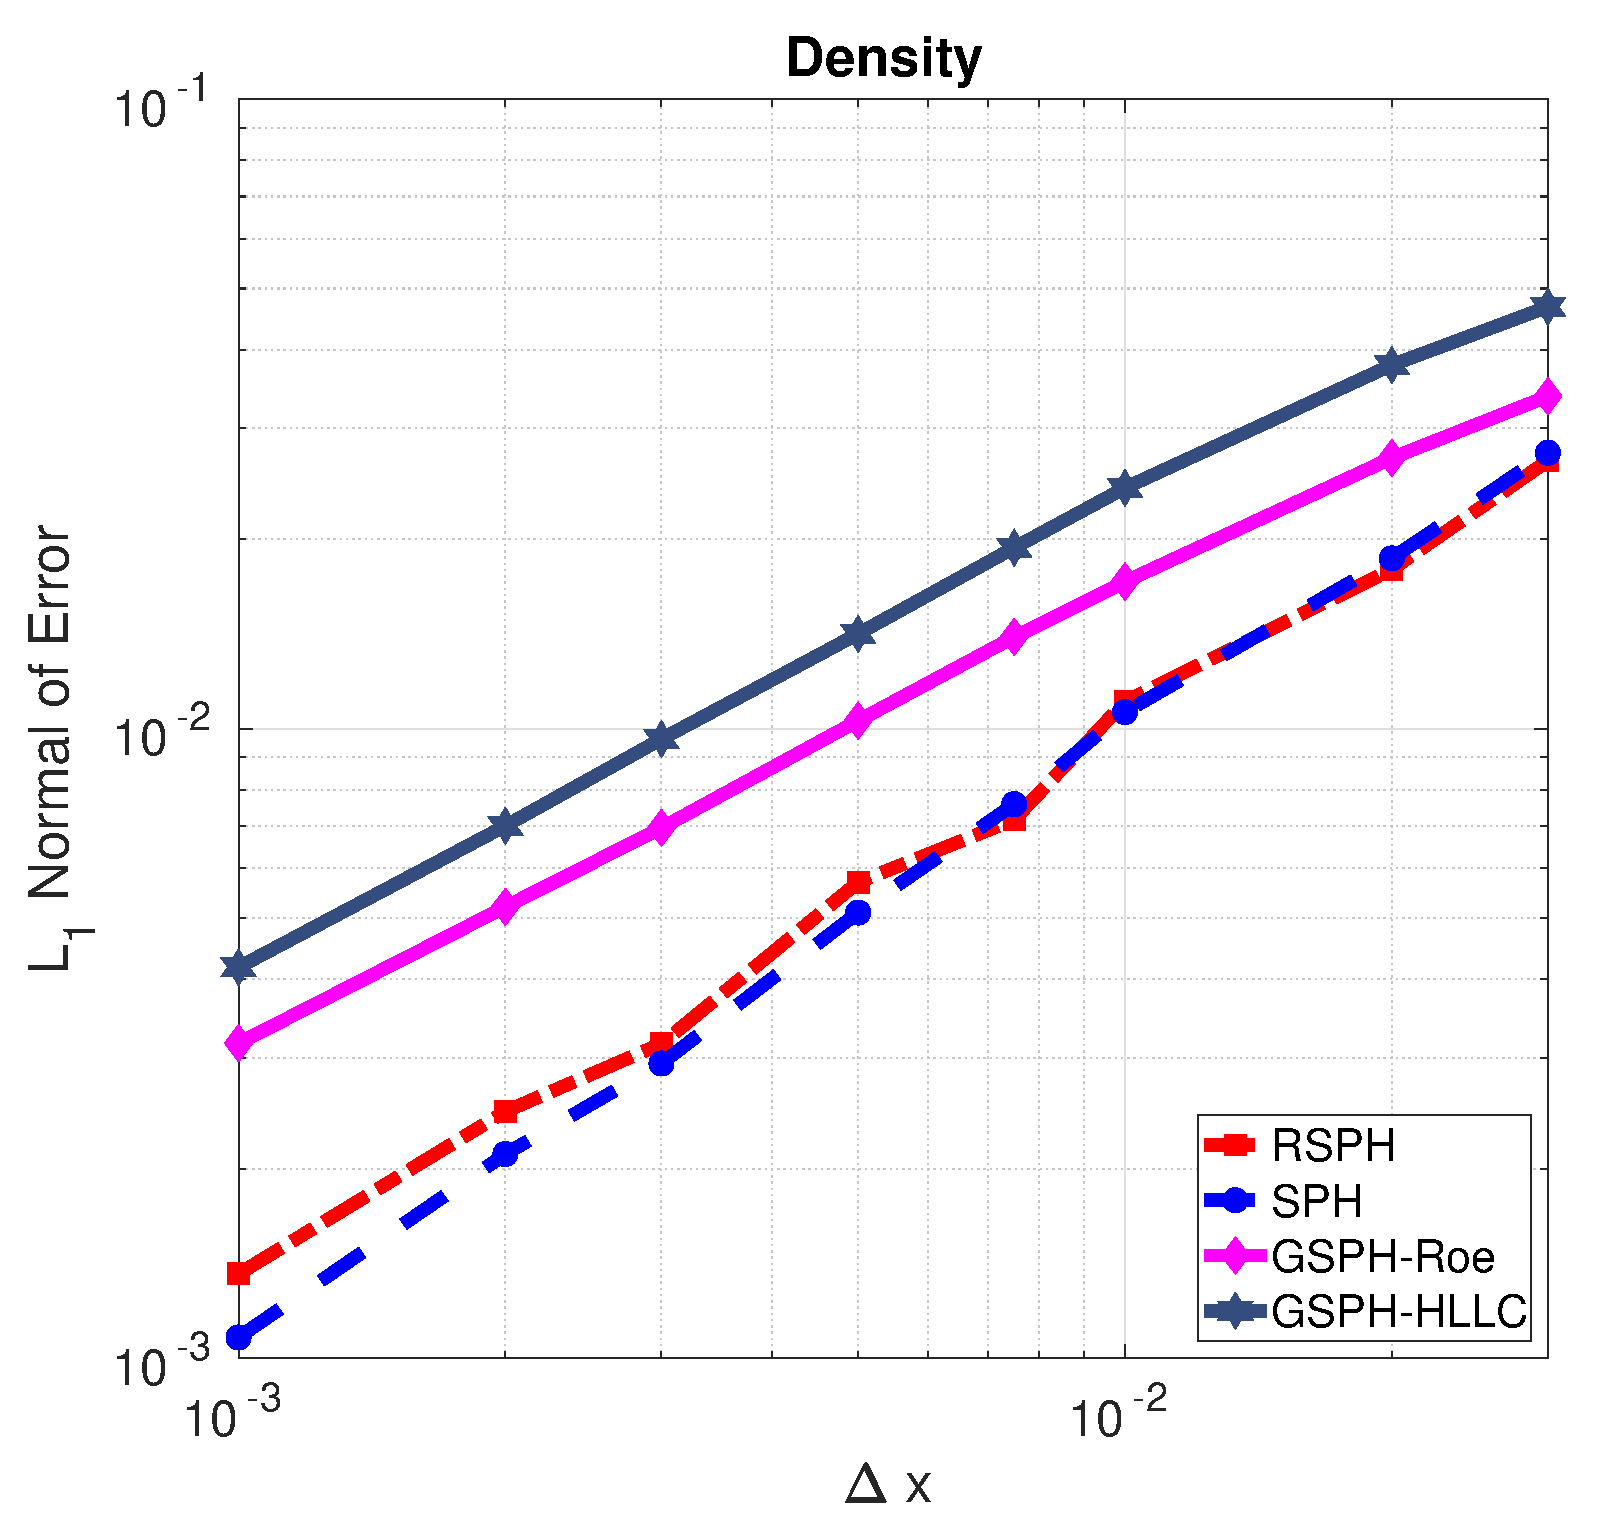
\includegraphics[width=0.99 \textwidth]{./Chapter-4/Figures/Accuracy-des}
    \end{minipage}%
    \begin{minipage}{.332 \textwidth}
        \centering
        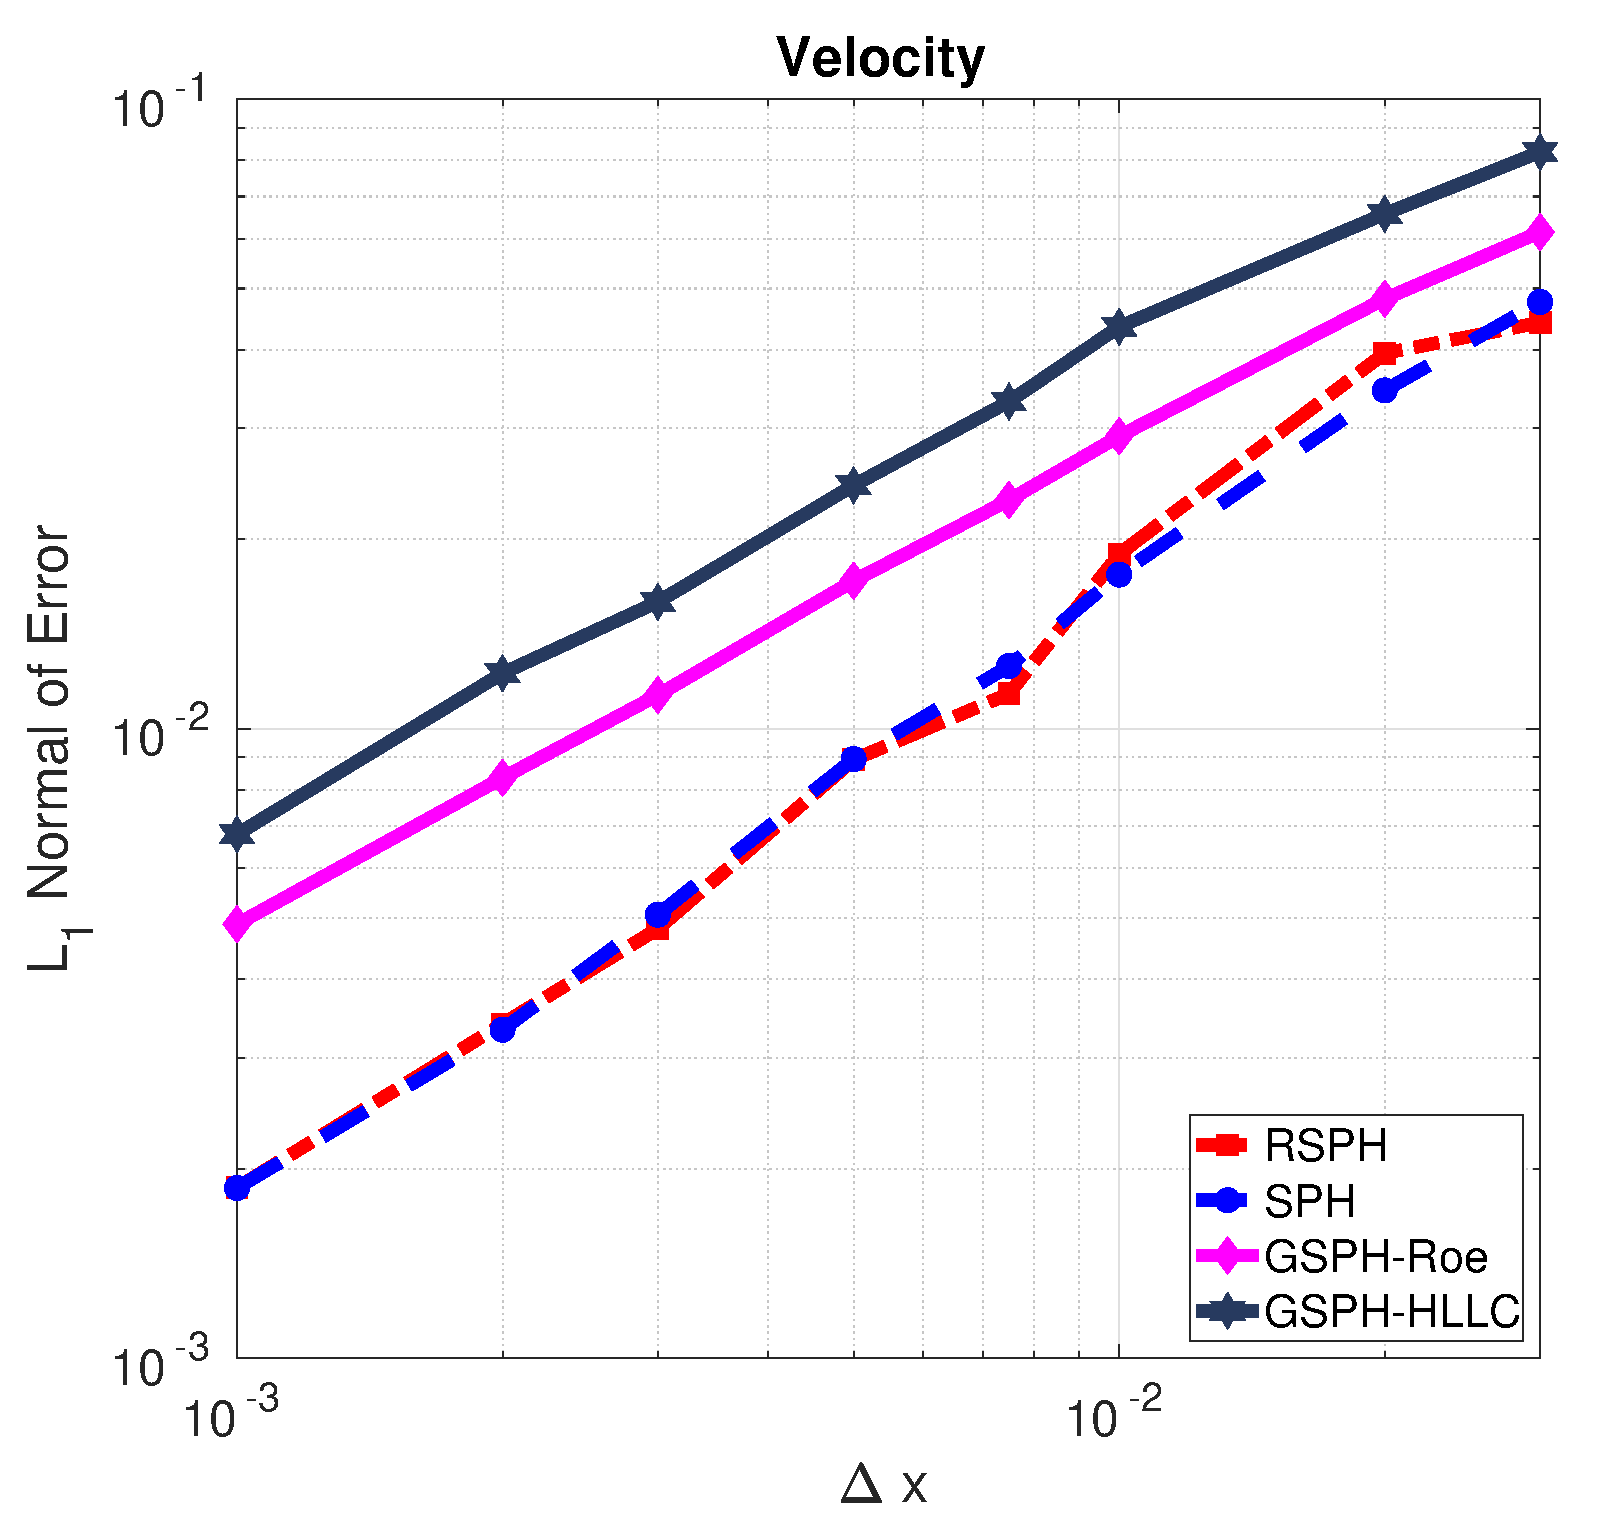
\includegraphics[width=0.99 \textwidth]{./Chapter-4/Figures/Accuracy-vel}
    \end{minipage}%
    \begin{minipage}{.332\textwidth}
        \centering
        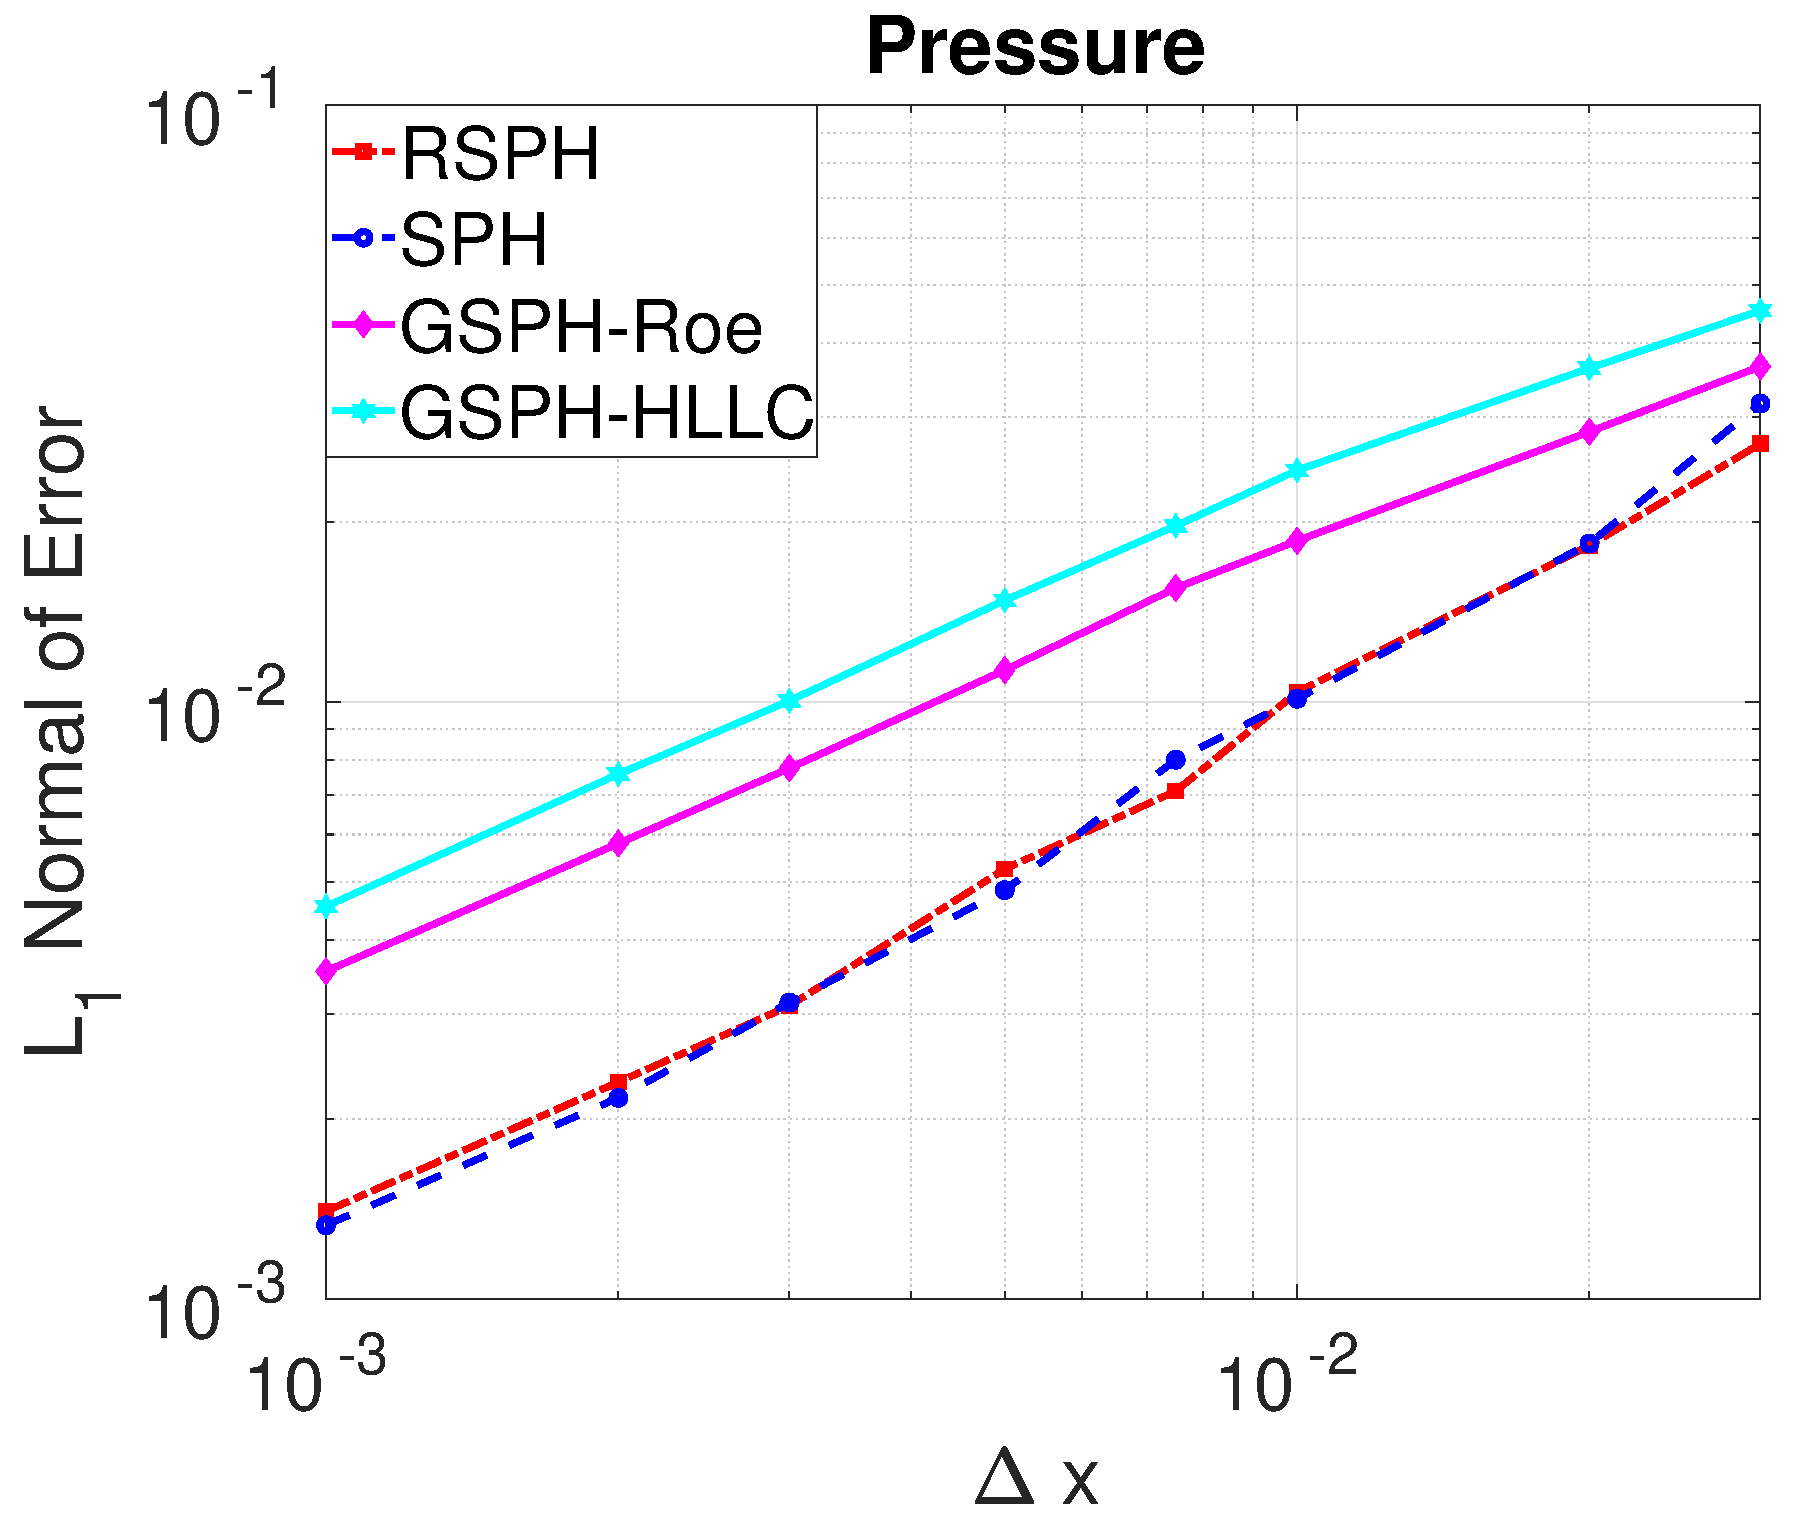
\includegraphics[width=0.99 \textwidth]{./Chapter-4/Figures/Accuracy-pre}
    \end{minipage}%  
    \caption{ $L_1$ norm errors for 1D shock tube test (test1) for RSPH, standard SPH, GSPH using Roe Riemann solver and GSPH using HLLC Riemann Solver.  GSPH with the HLLC approximate Riemann solver exhibits the same convergence rate (around 1) but quantitatively larger errors than that with Roe Riemann solver. RSPH and standard SPH shows same rate of convergence and almost same amount of error.}
    \label{fig:Accuracy-test1}
\end{figure}
 
\subsection{Comprehensive 1D tests} \label{sec:comprehensive-1d-tests}
Comprehensive tests are presented in this section to check how well does RSPH work for different situations. Input parameters for each tests is given in Table \ref{tab:1D-shock-input_parameters}.
The results are shown in Fig. \ref{fig:RCM-GSPH-Sod} $\sim$ Fig. \ref{fig:RCM-strong-blast}. $x$ axis in these plots are normalized by the terminal time $t_f$. We observe that RSPH is able to correctly predict the position and magnitude of all waves for all tests. A jump of specific internal energy at the origin is observed in Sj$\ddot{o}$green test. However, such jump is a common issue of SPH schemes and has been reported in many other tests (see, for example, \citep{monaghan1997sph,cha2003implementations,puri2014approximate})
In addition, a noticeable spike can be observed near the contact discontinuity. Similar spike is observed in GSPH simulation \citep{puri2014comparison}. %Such spike is evident in the FVM solution as well and is perhaps an artifice of the Lagrangian nature of the two schemes. 
\citet{noh1987errors} proposed to adding a small amount of thermal conduction to ameliorate the spike and has been applied in blast-wave test using GSPH \citep{puri2014comparison}. We did not adopt such strategy in our simulation.
Due to less amount of dissipation, numerical fluctuations persist in all simulation results. For the strong blast test and double shock test, such fluctuations become more obvious than other tests, even though, the magnitude of fluctuations is within an acceptable range.

\begin{figure}
    \centering
    \begin{minipage}{.415\textwidth}
        \centering
        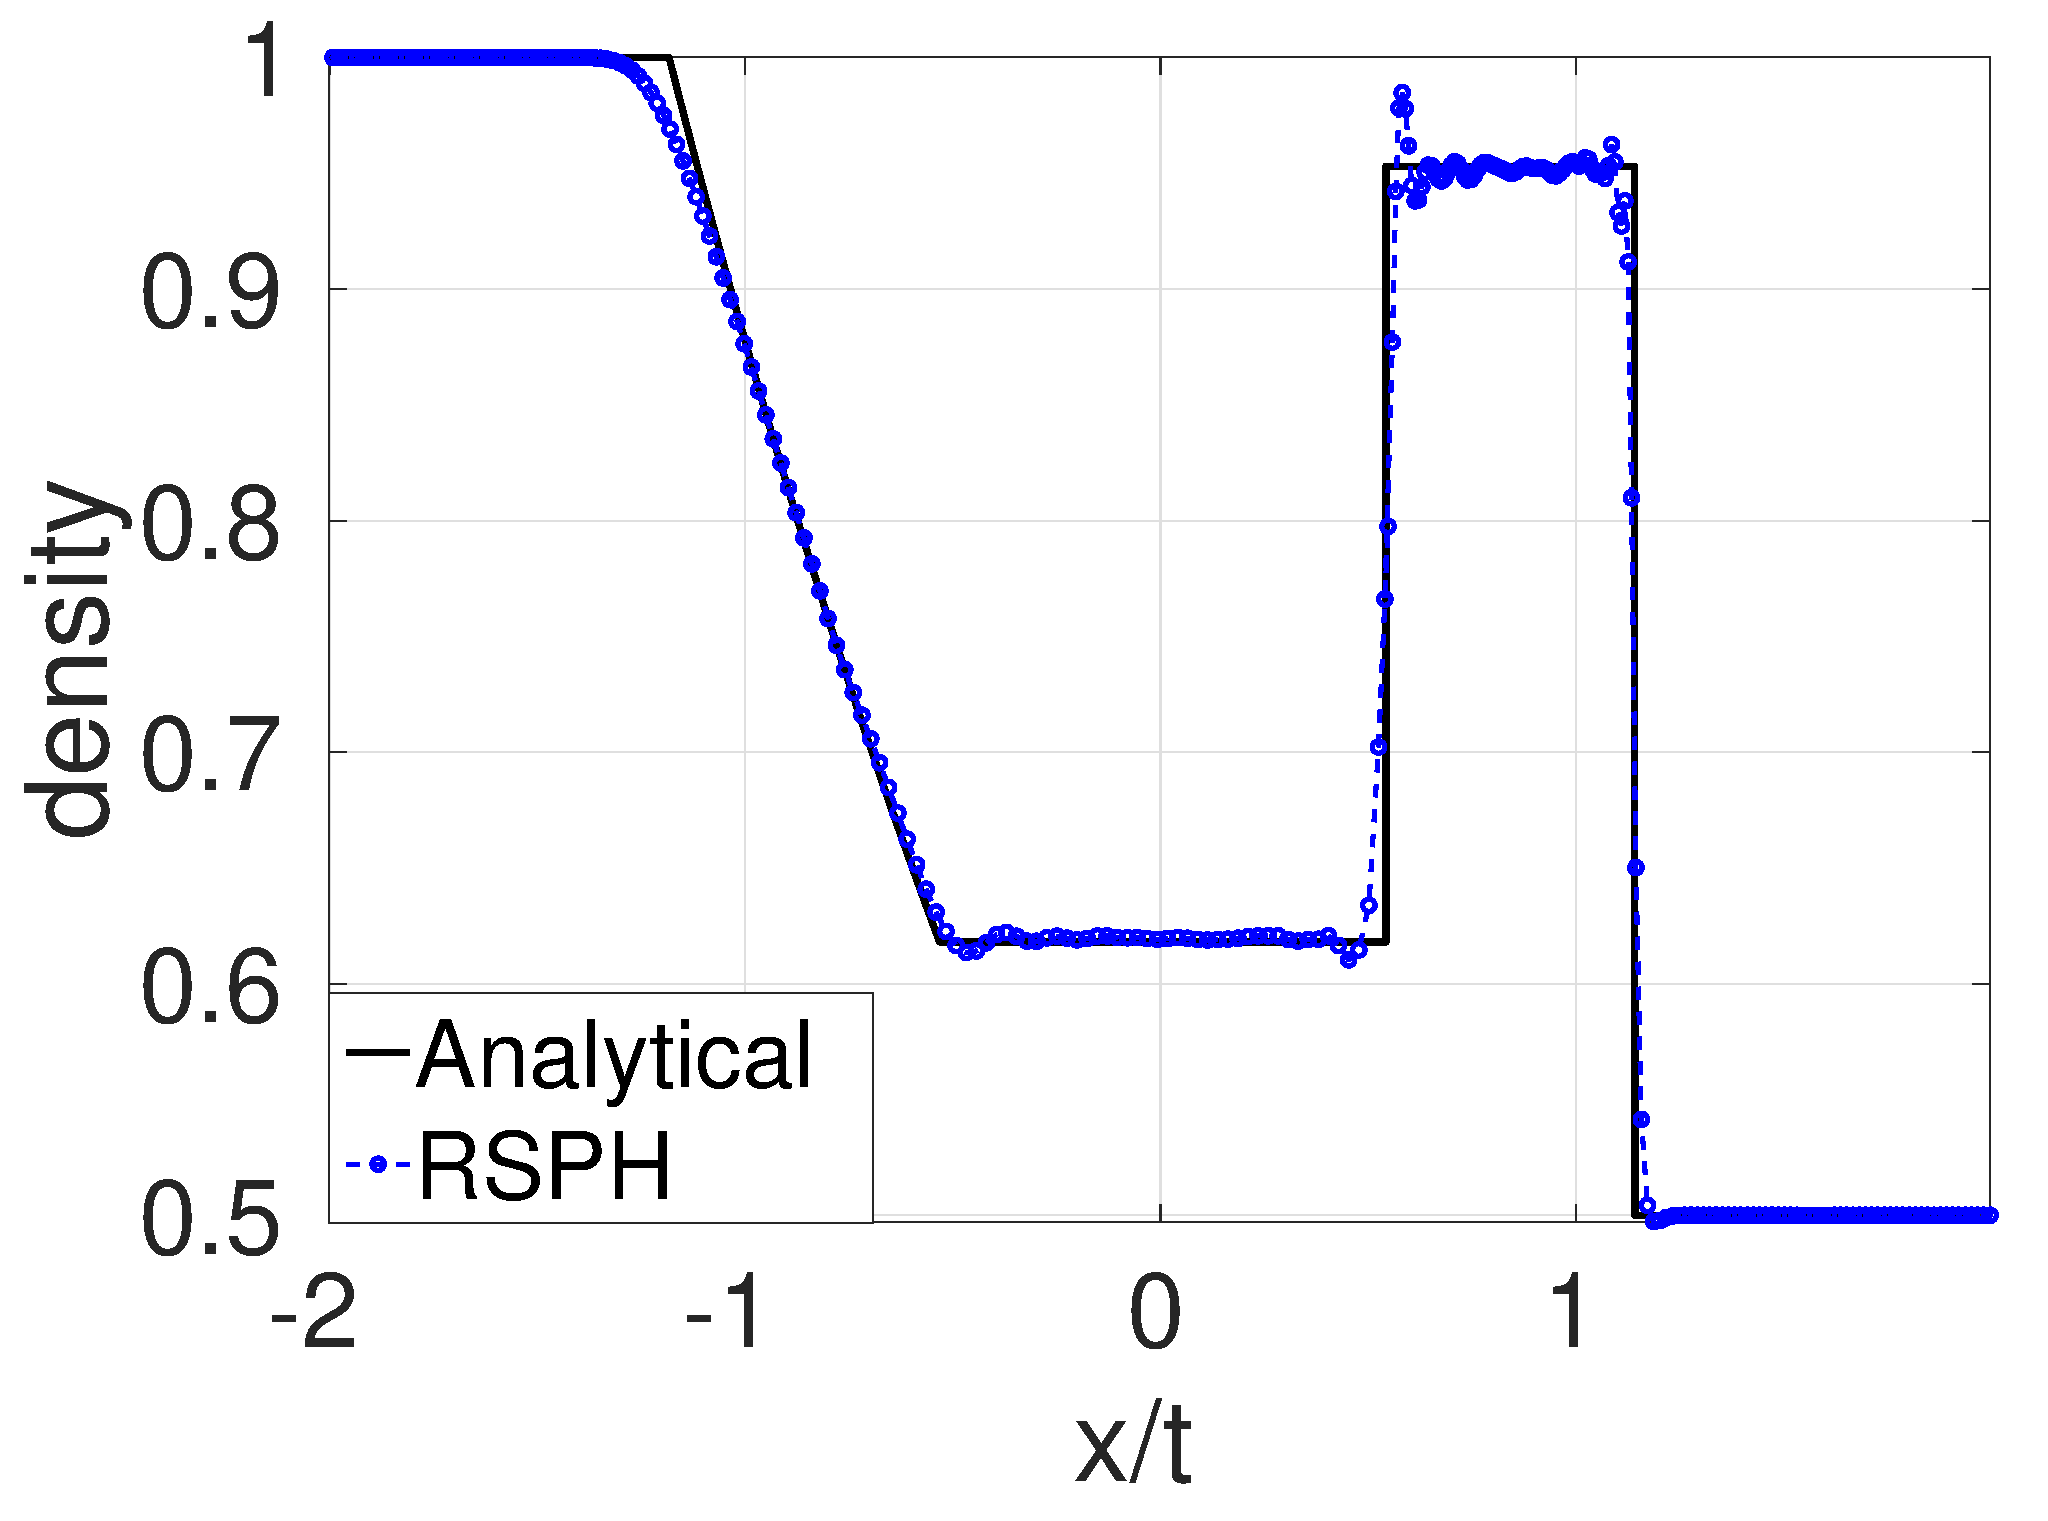
\includegraphics[width=0.99 \textwidth]{./Chapter-4/Figures/GSPH-Sod/GRod-RCM-rho}
    \end{minipage}%
    \begin{minipage}{.415 \textwidth}
        \centering
        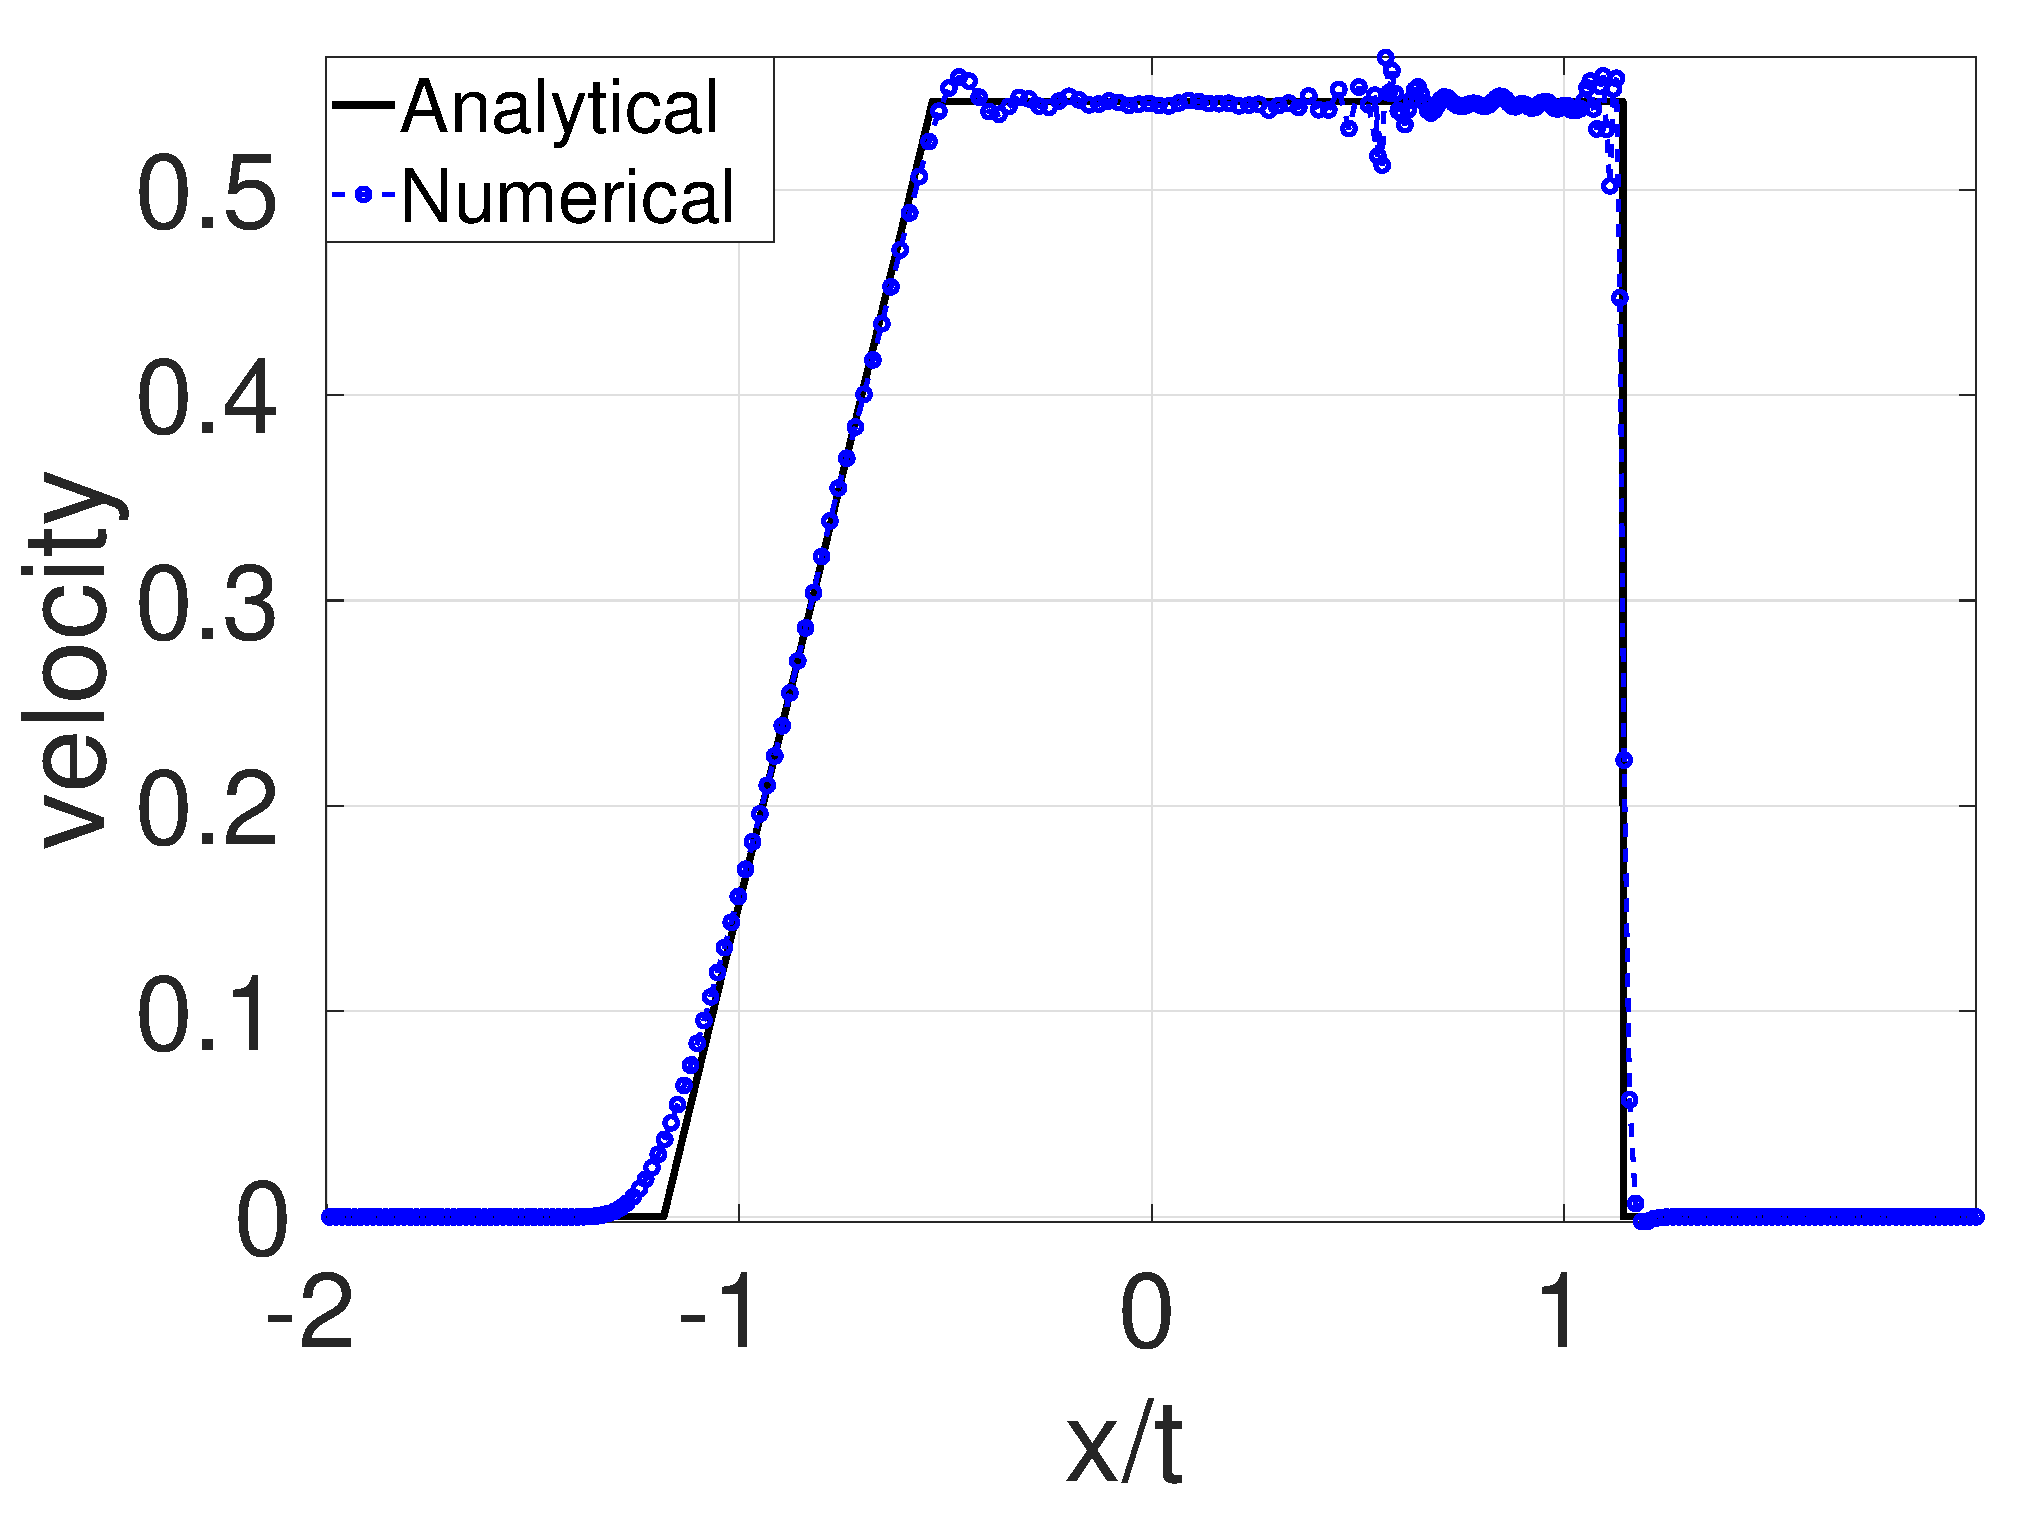
\includegraphics[width=0.99 \textwidth]{./Chapter-4/Figures/GSPH-Sod/GRod-RCM-v}
    \end{minipage}% 
    \\
    \begin{minipage}{.415\textwidth}
        \centering
        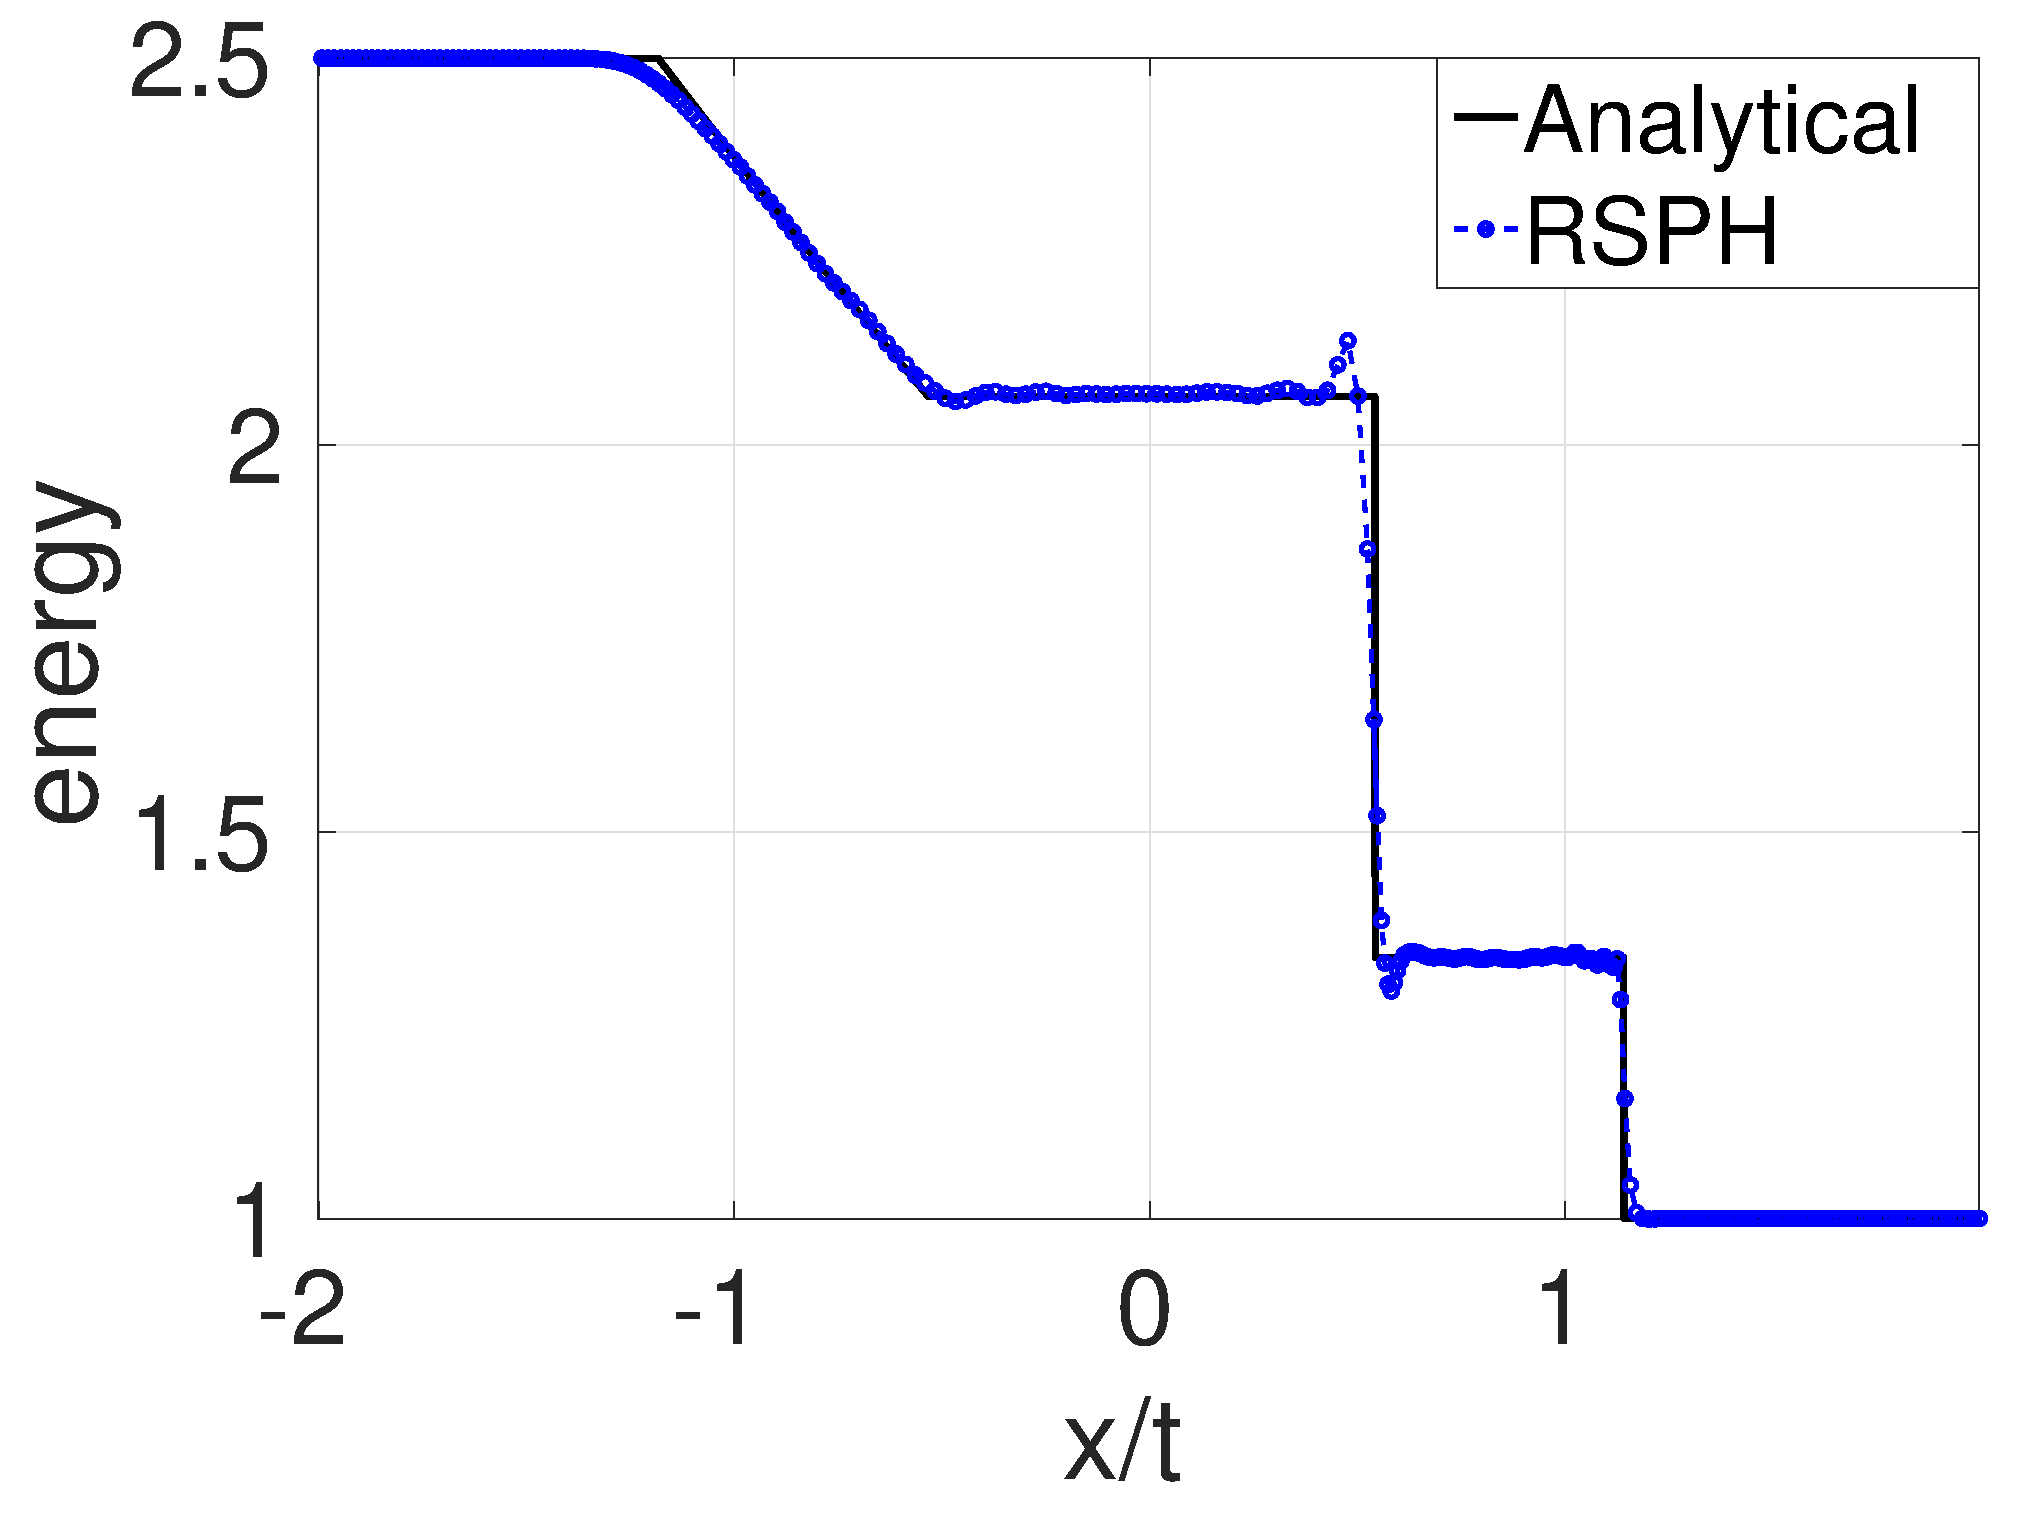
\includegraphics[width=0.99 \textwidth]{./Chapter-4/Figures/GSPH-Sod/GRod-RCM-e}
    \end{minipage}%
    \begin{minipage}{.415 \textwidth}
        \centering
        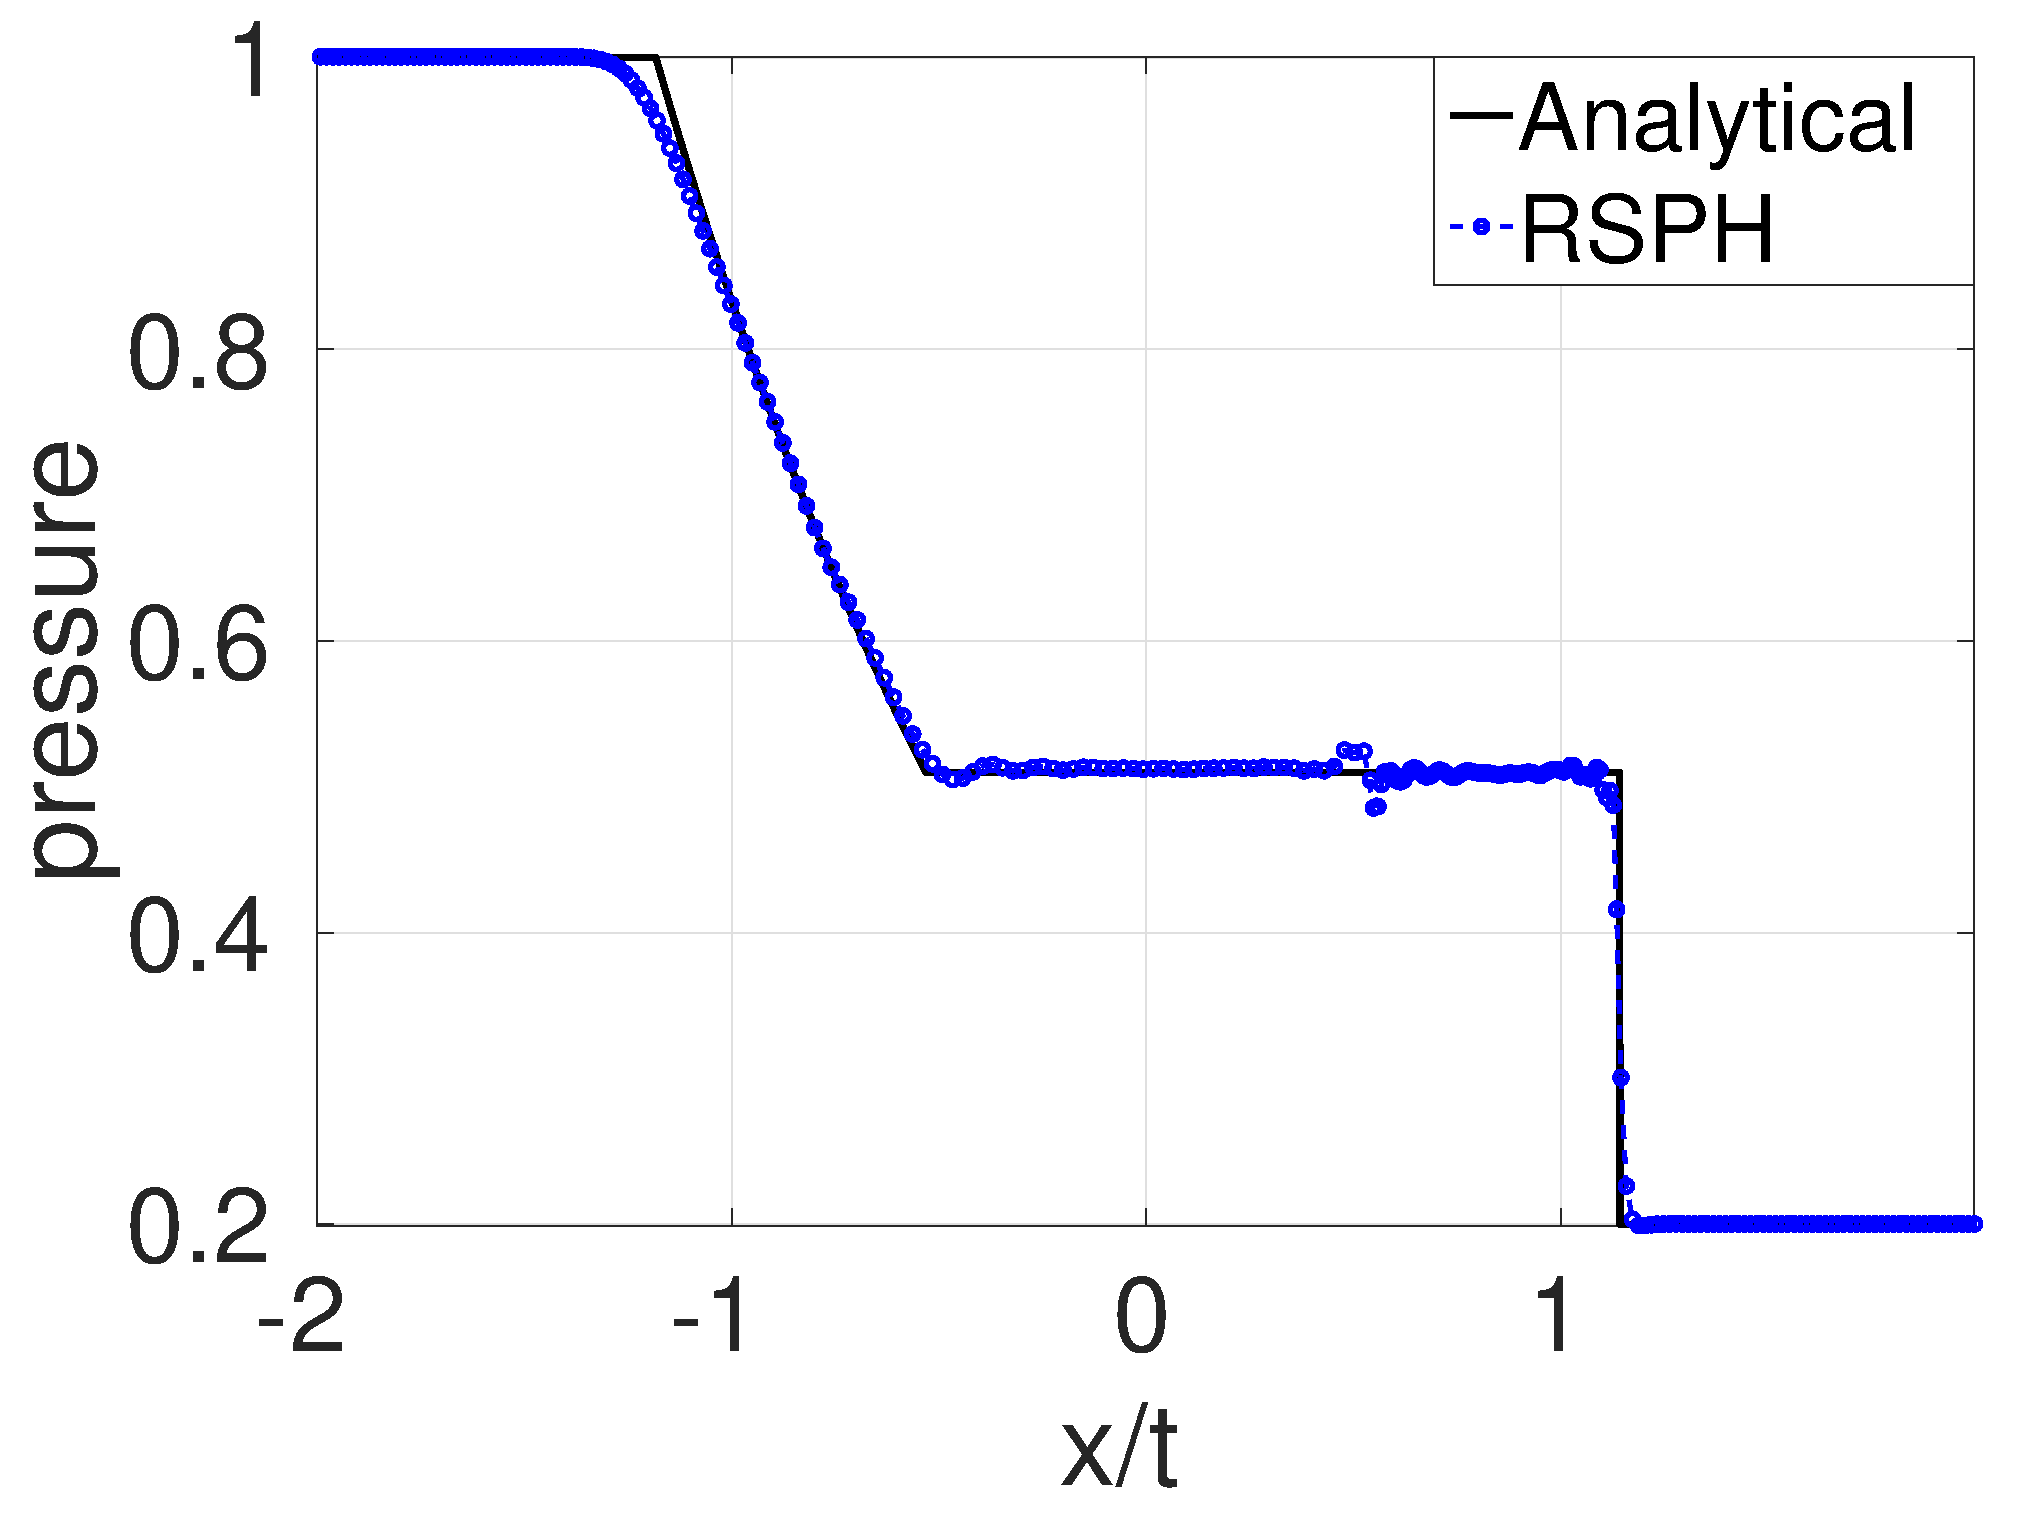
\includegraphics[width=0.99 \textwidth]{./Chapter-4/Figures/GSPH-Sod/GRod-RCM-p}
    \end{minipage}% 
    \caption{Results for test 2, a variation of Sod test. All physical properties are well re-produced except for some acceptable oscillations}
    \label{fig:RCM-GSPH-Sod}
\end{figure}

\begin{figure}
    \centering
    \begin{minipage}{.415\textwidth}
        \centering
        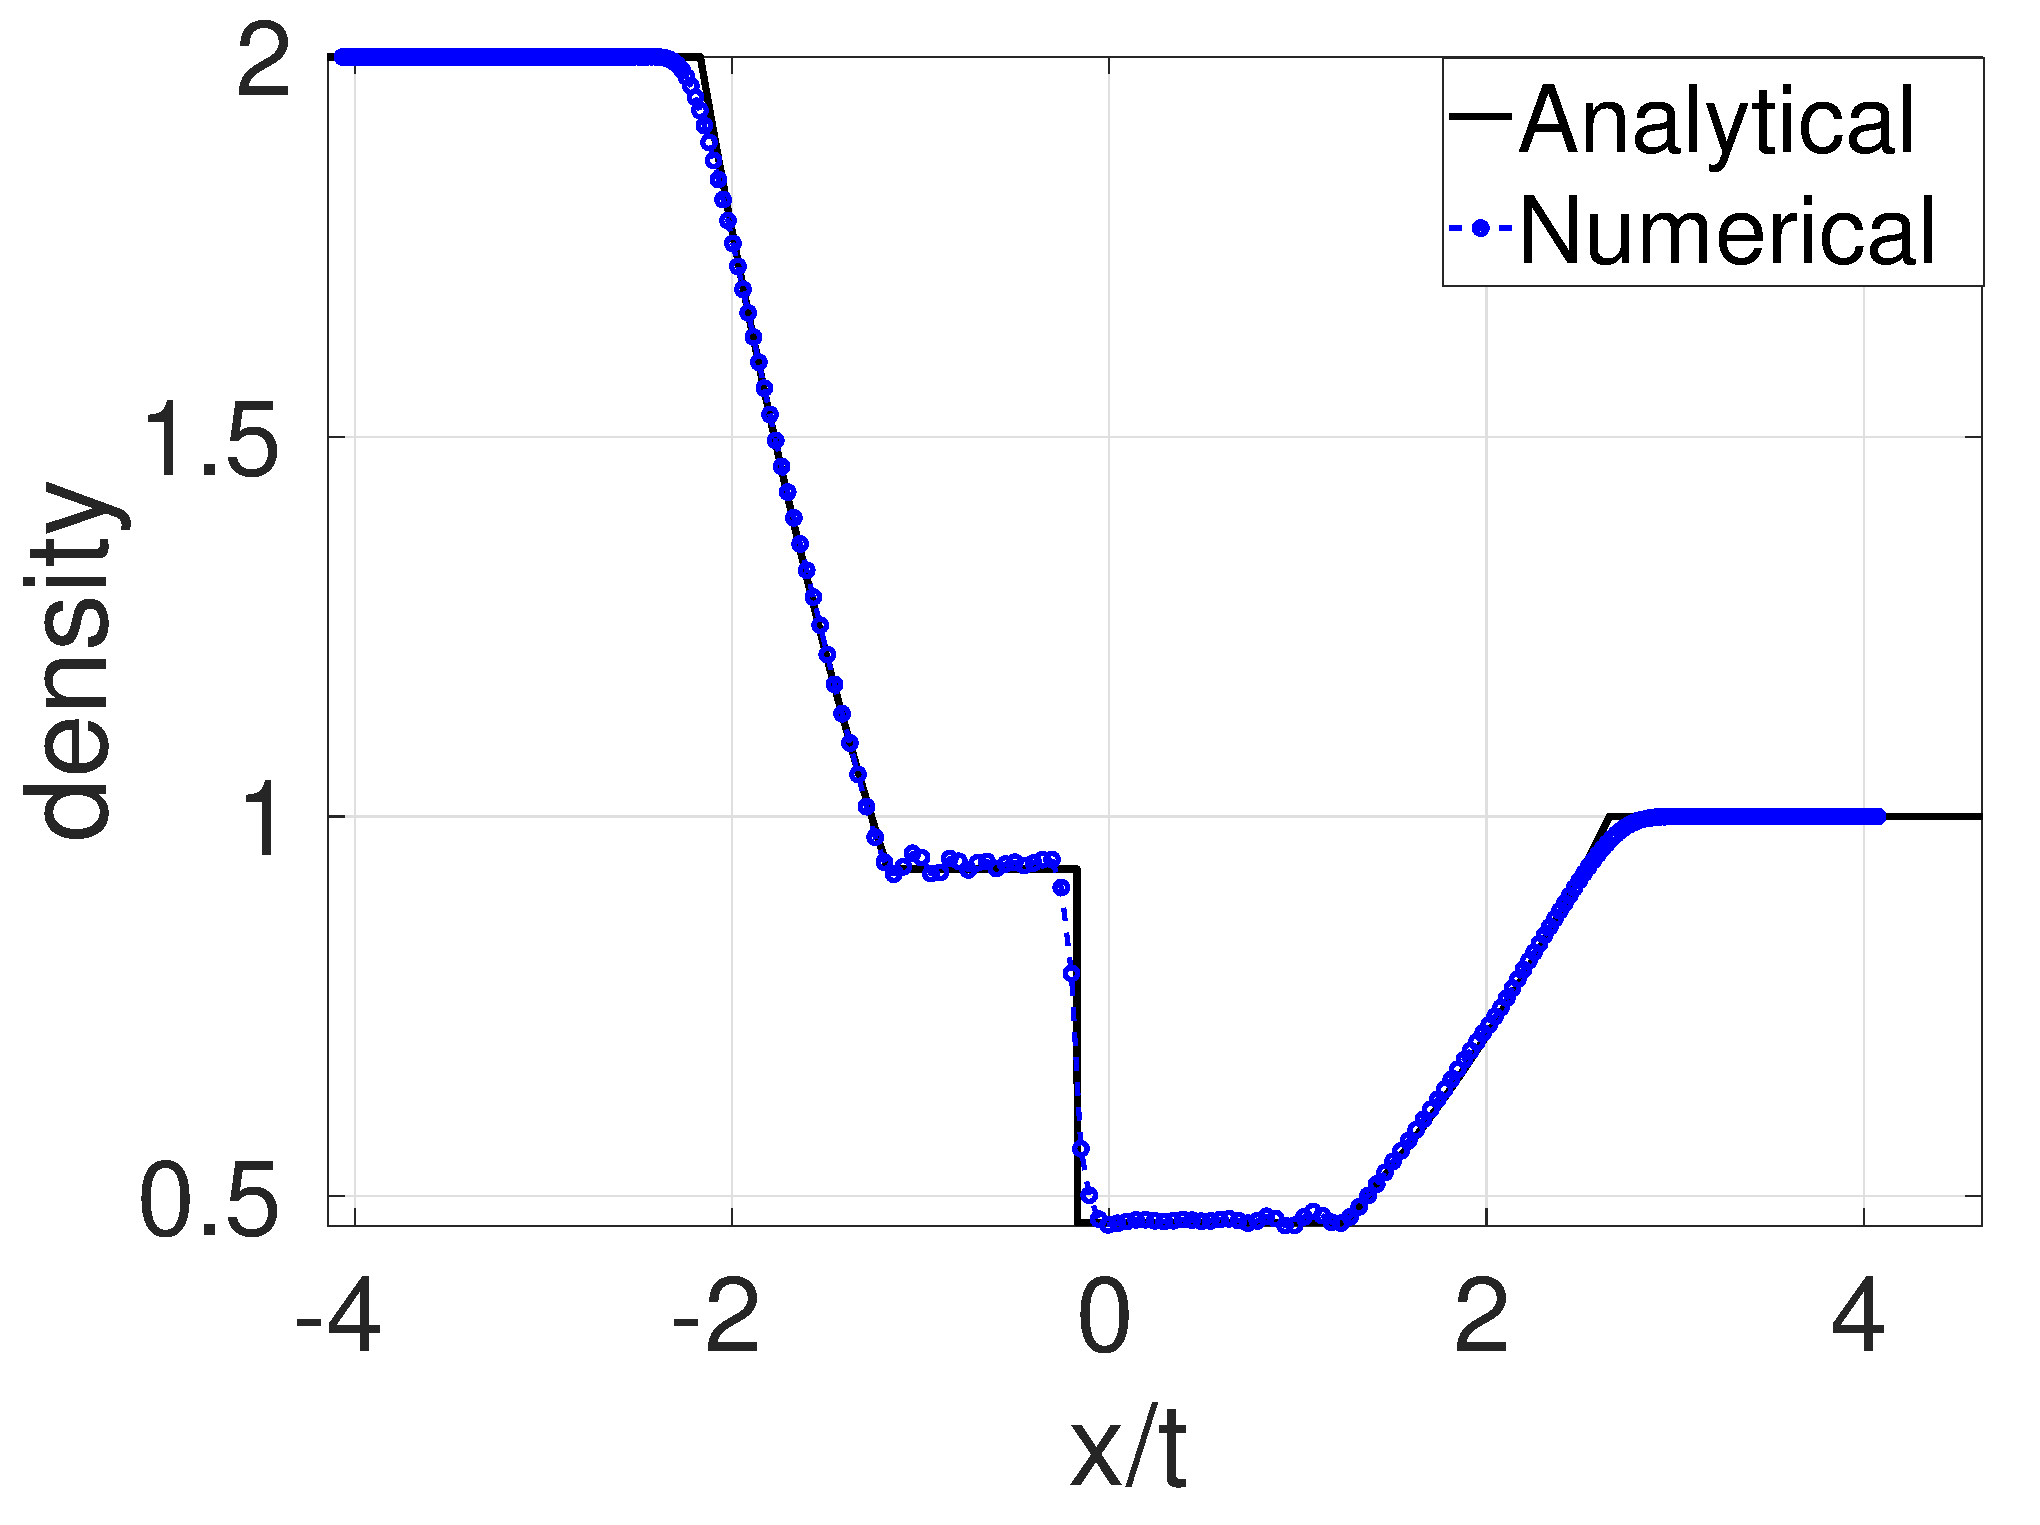
\includegraphics[width=0.99 \textwidth]{./Chapter-4/Figures/double_exp/Dexp-RCM-rho}
    \end{minipage}%
    \begin{minipage}{.415 \textwidth}
        \centering
        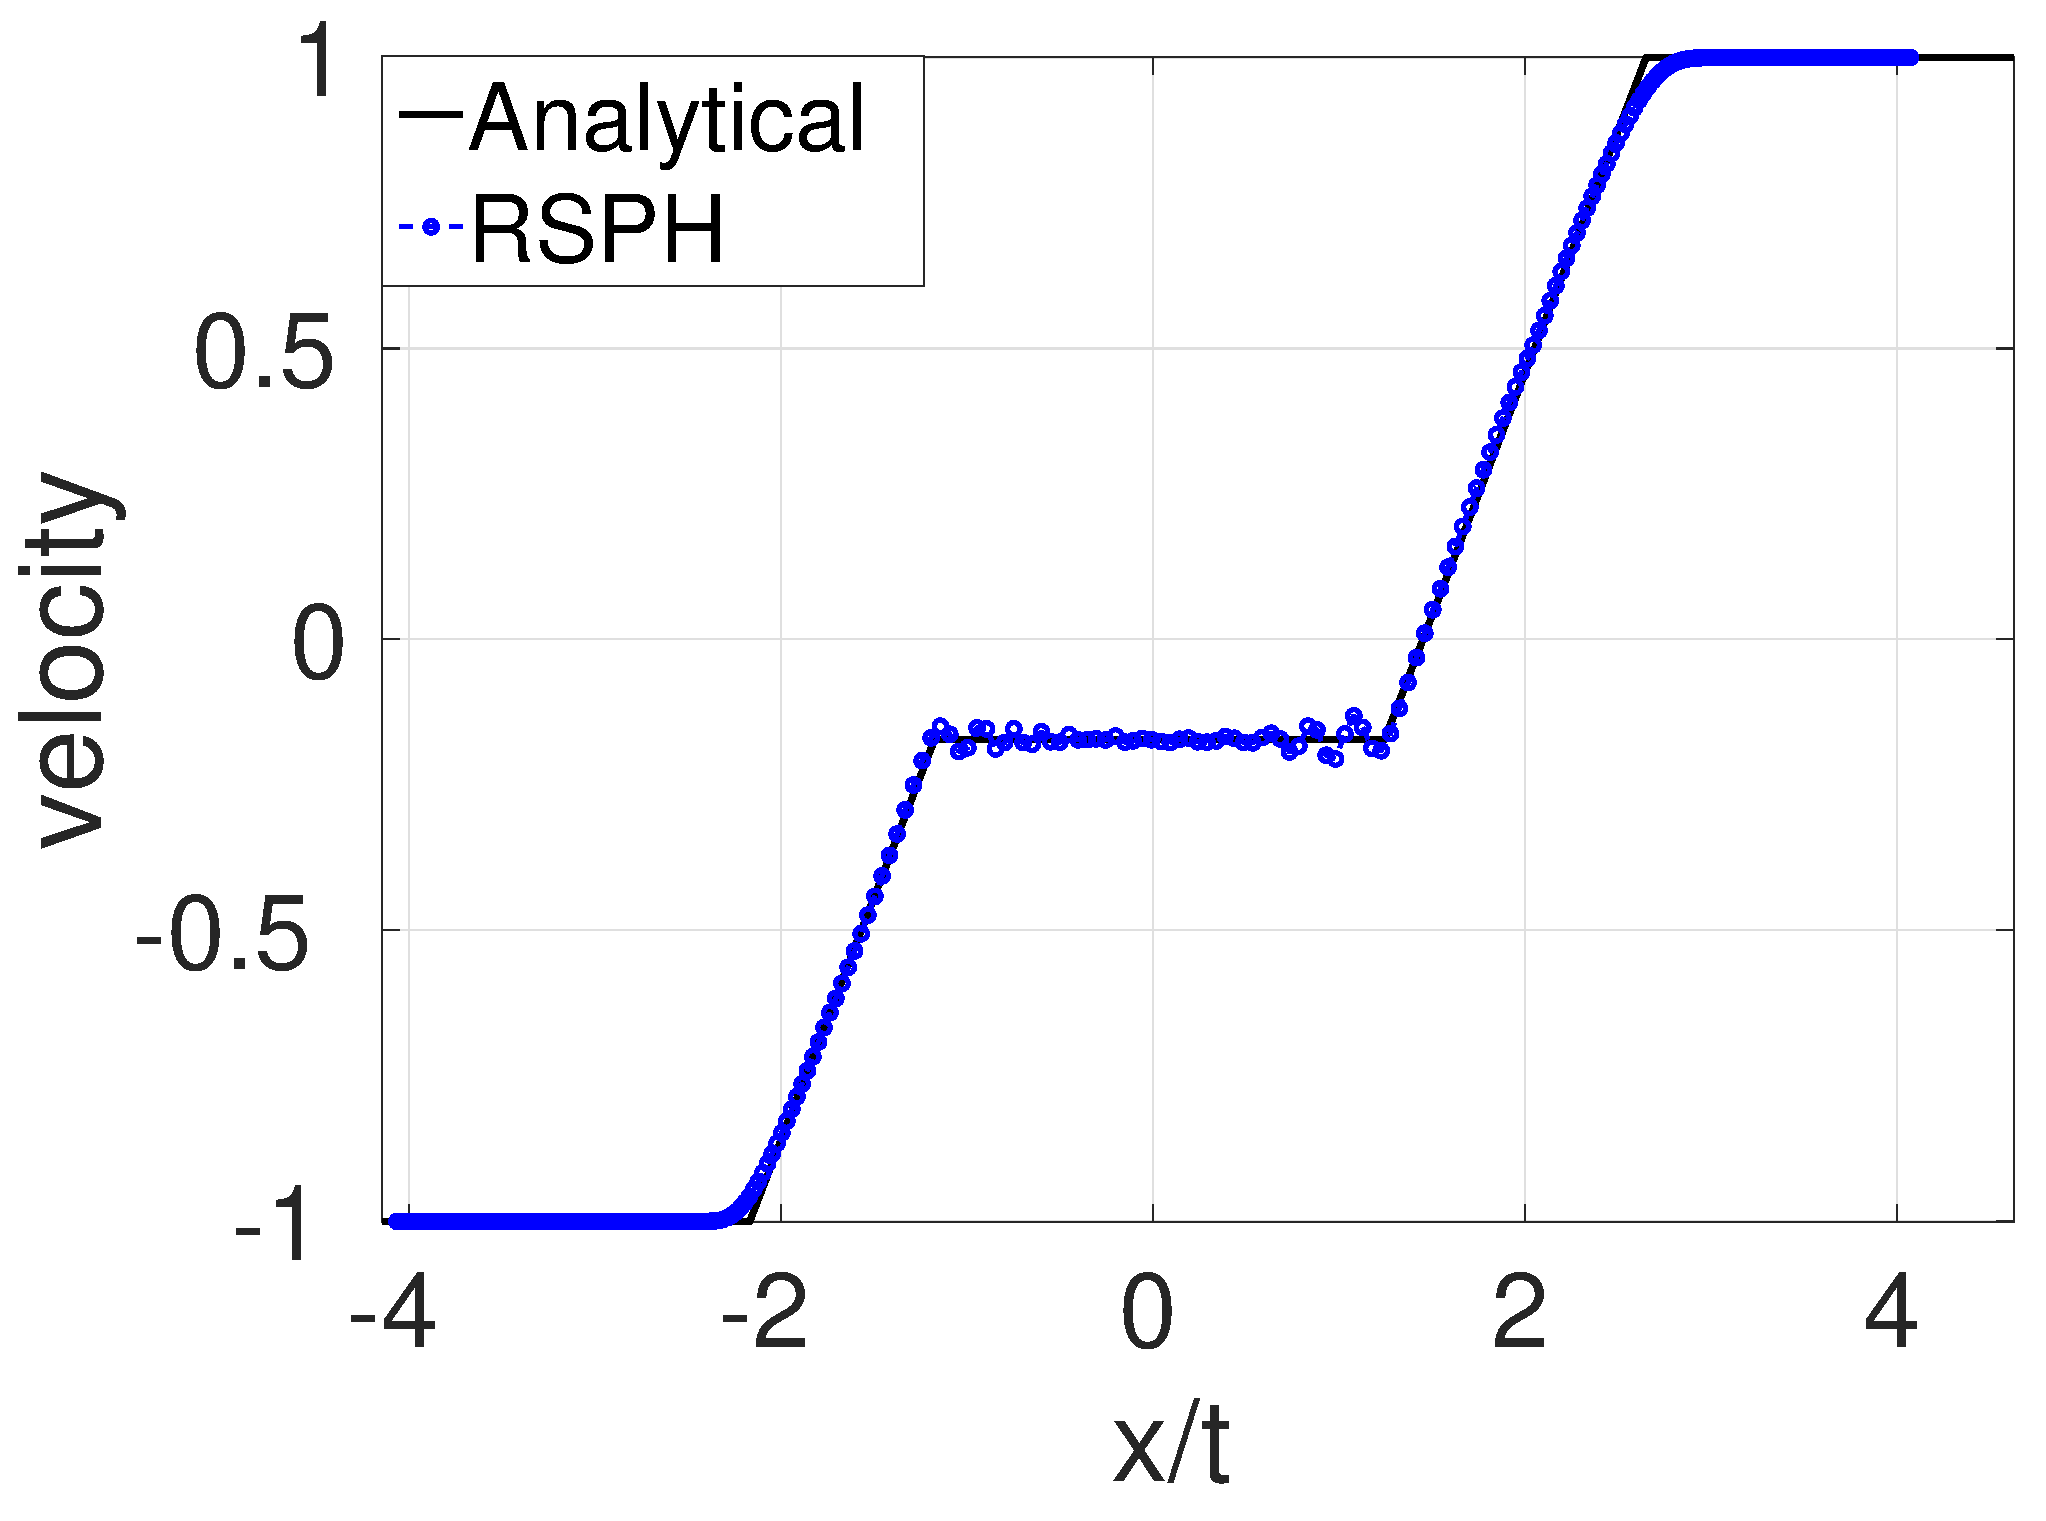
\includegraphics[width=0.99 \textwidth]{./Chapter-4/Figures/double_exp/Dexp-RCM-v}
    \end{minipage}%
    \\
    \begin{minipage}{.415\textwidth}
        \centering
        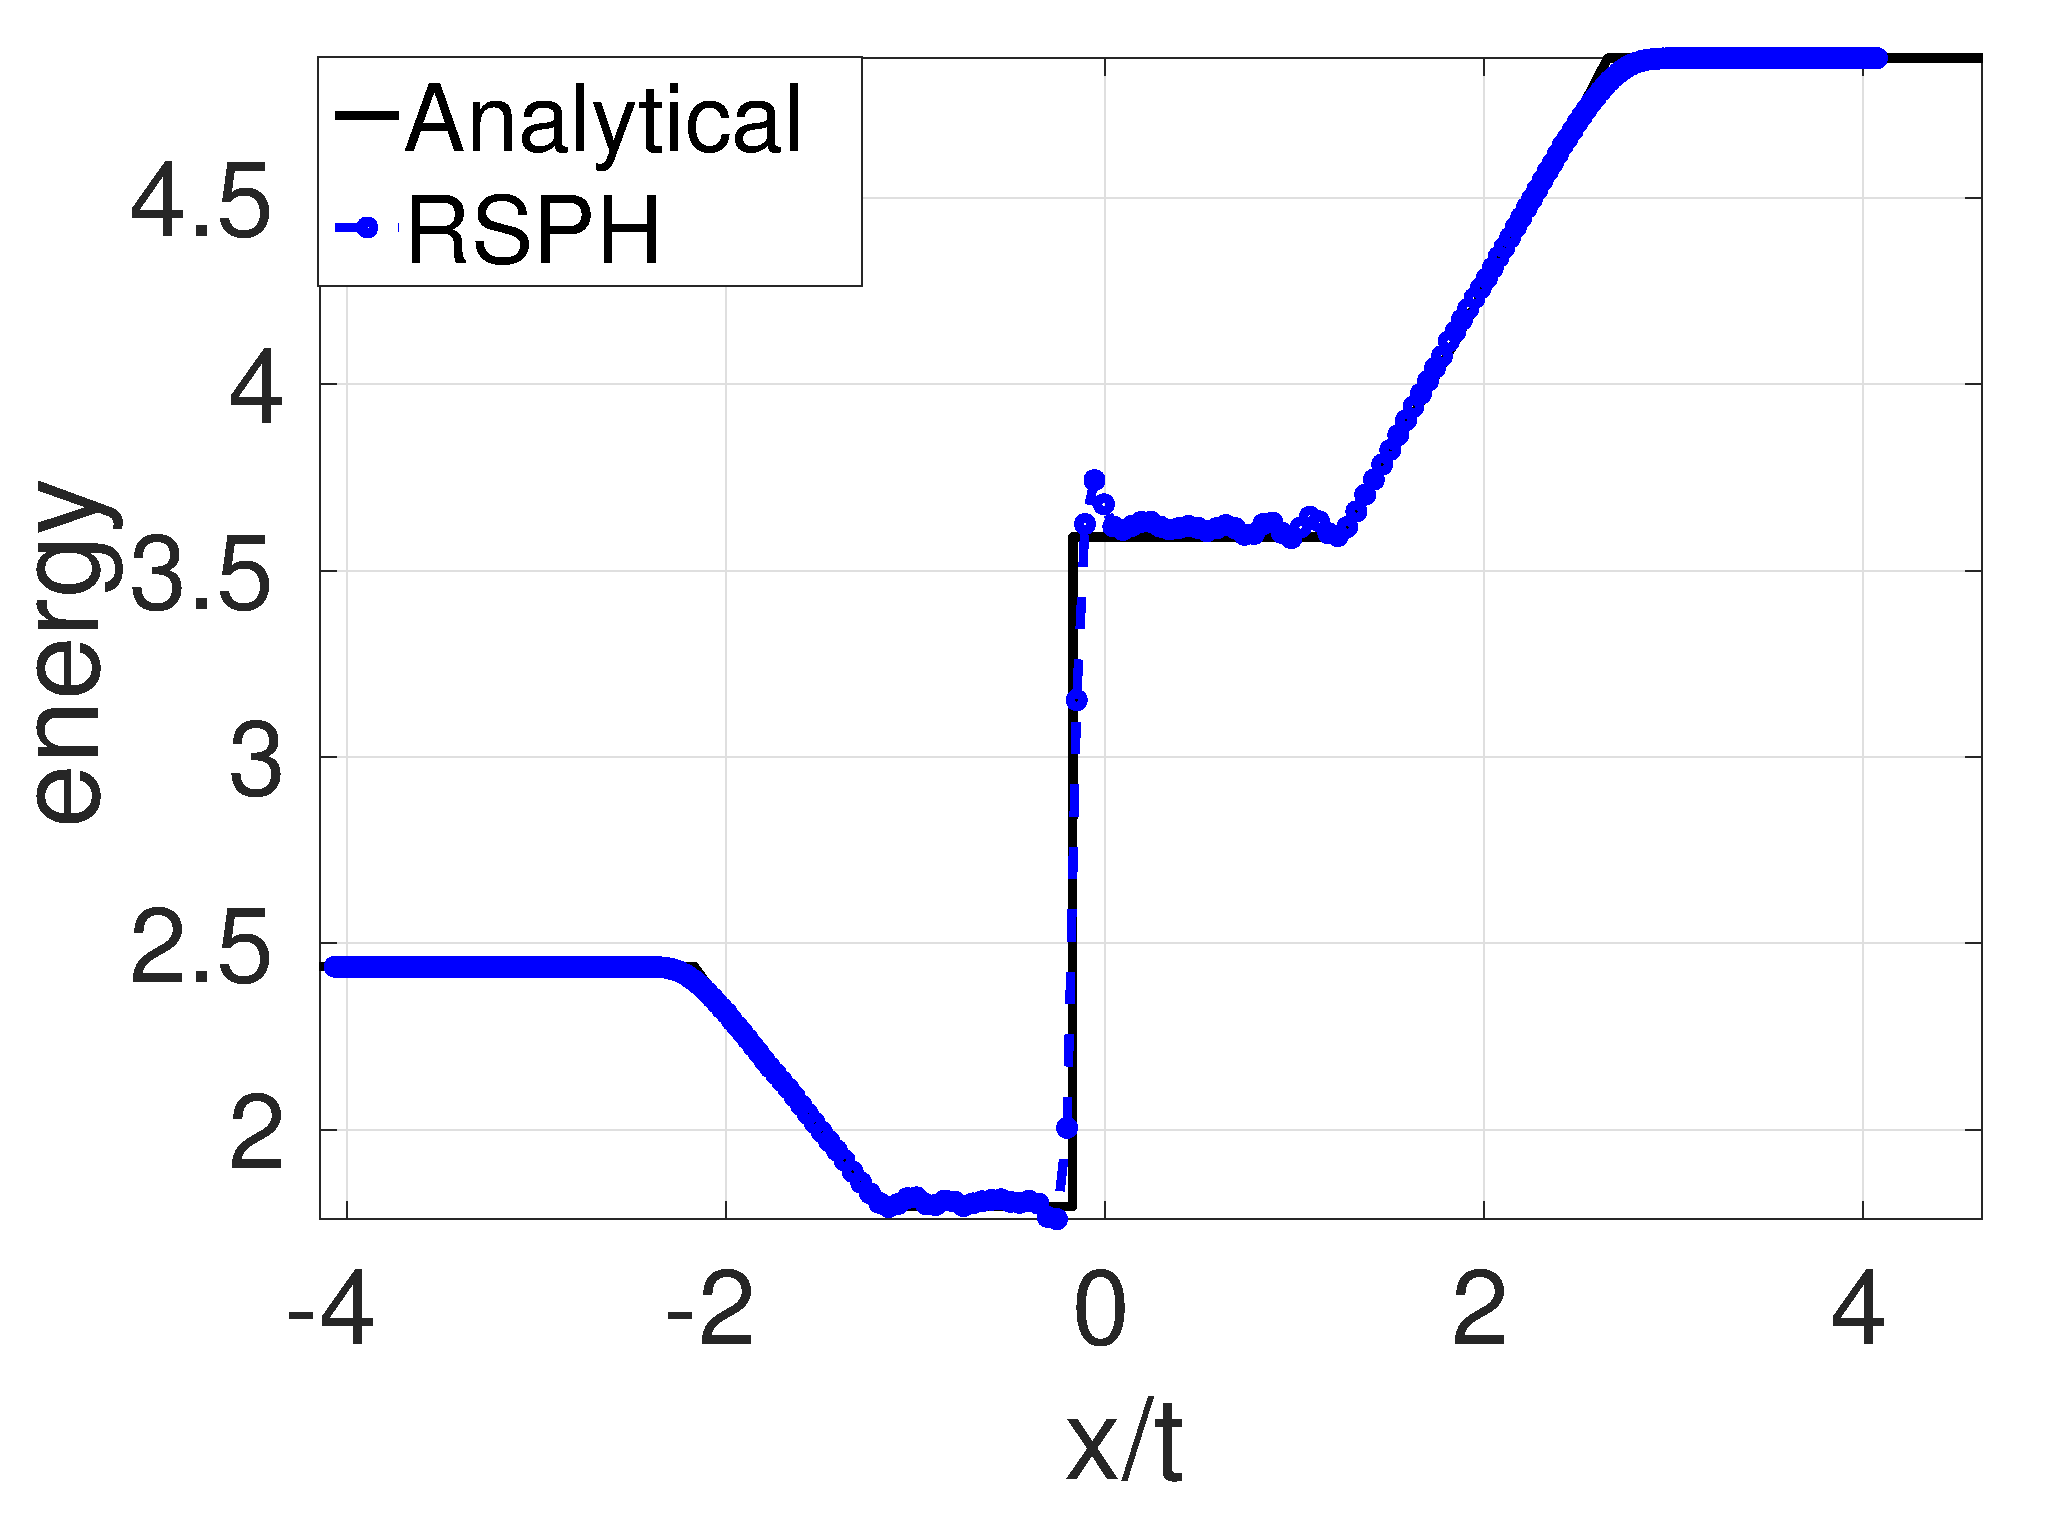
\includegraphics[width=0.99 \textwidth]{./Chapter-4/Figures/double_exp/Dexp-RCM-e}
    \end{minipage}%
    \begin{minipage}{.415 \textwidth}
        \centering
        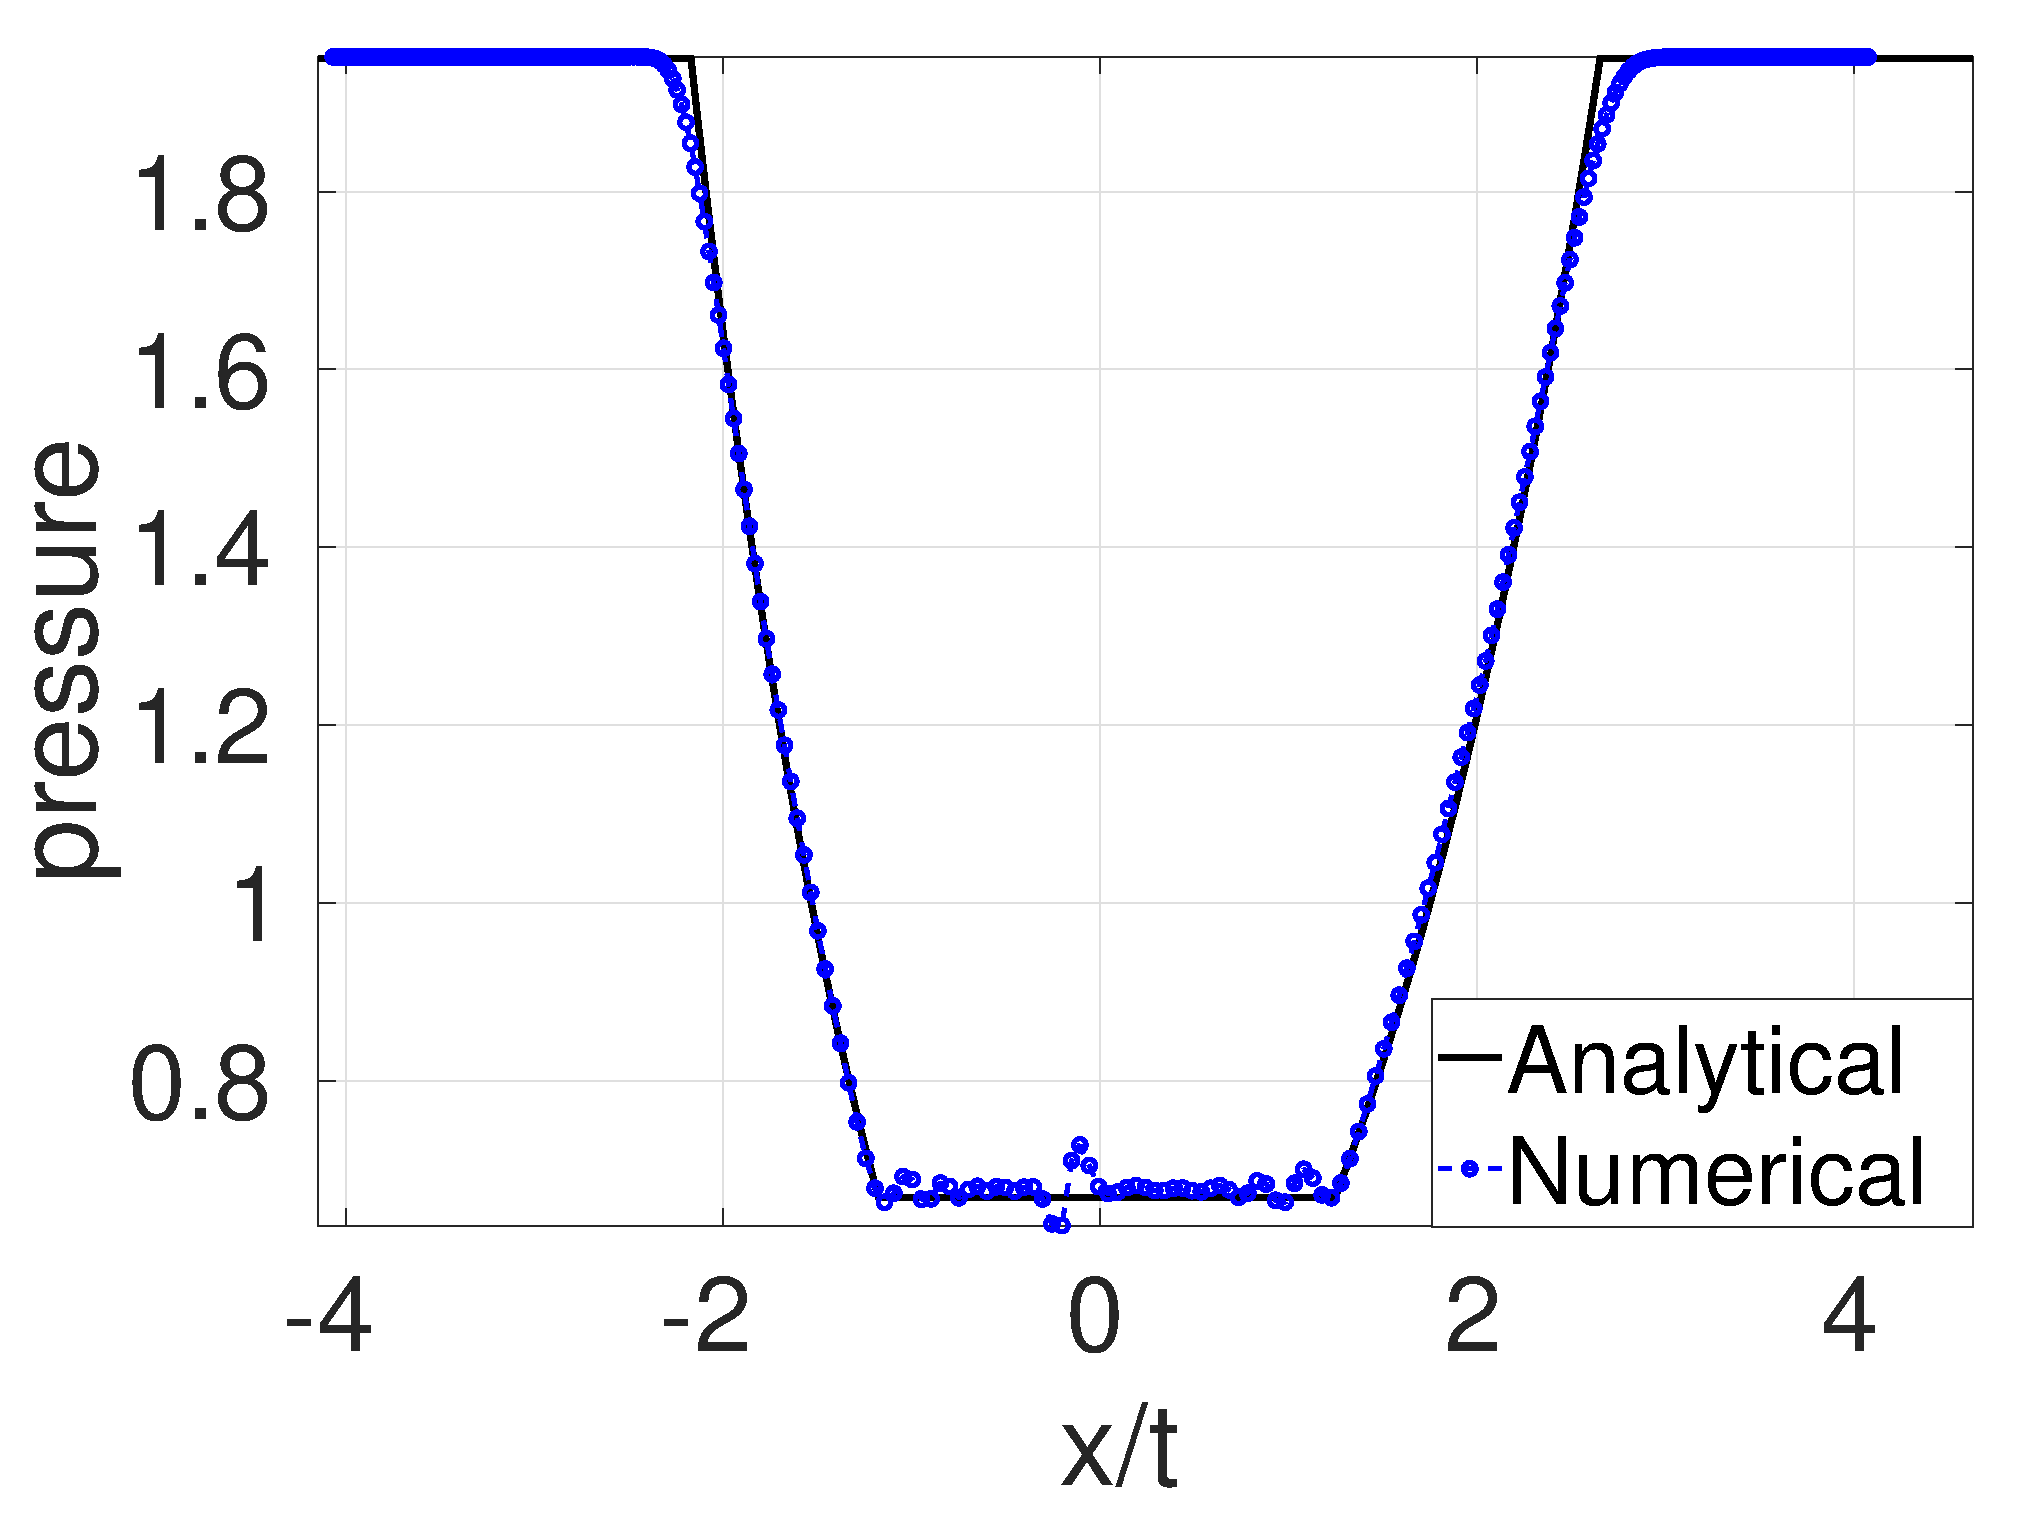
\includegraphics[width=0.99 \textwidth]{./Chapter-4/Figures/double_exp/Dexp-RCM-p}
    \end{minipage}% 
    \caption{Results for test 3, the double expansion case. All physical properties are well re-produced except for some oscillations}
    \label{fig:RCM-double-expansion}
\end{figure}

\begin{figure}
    \centering
    \begin{minipage}{.415\textwidth}
        \centering
        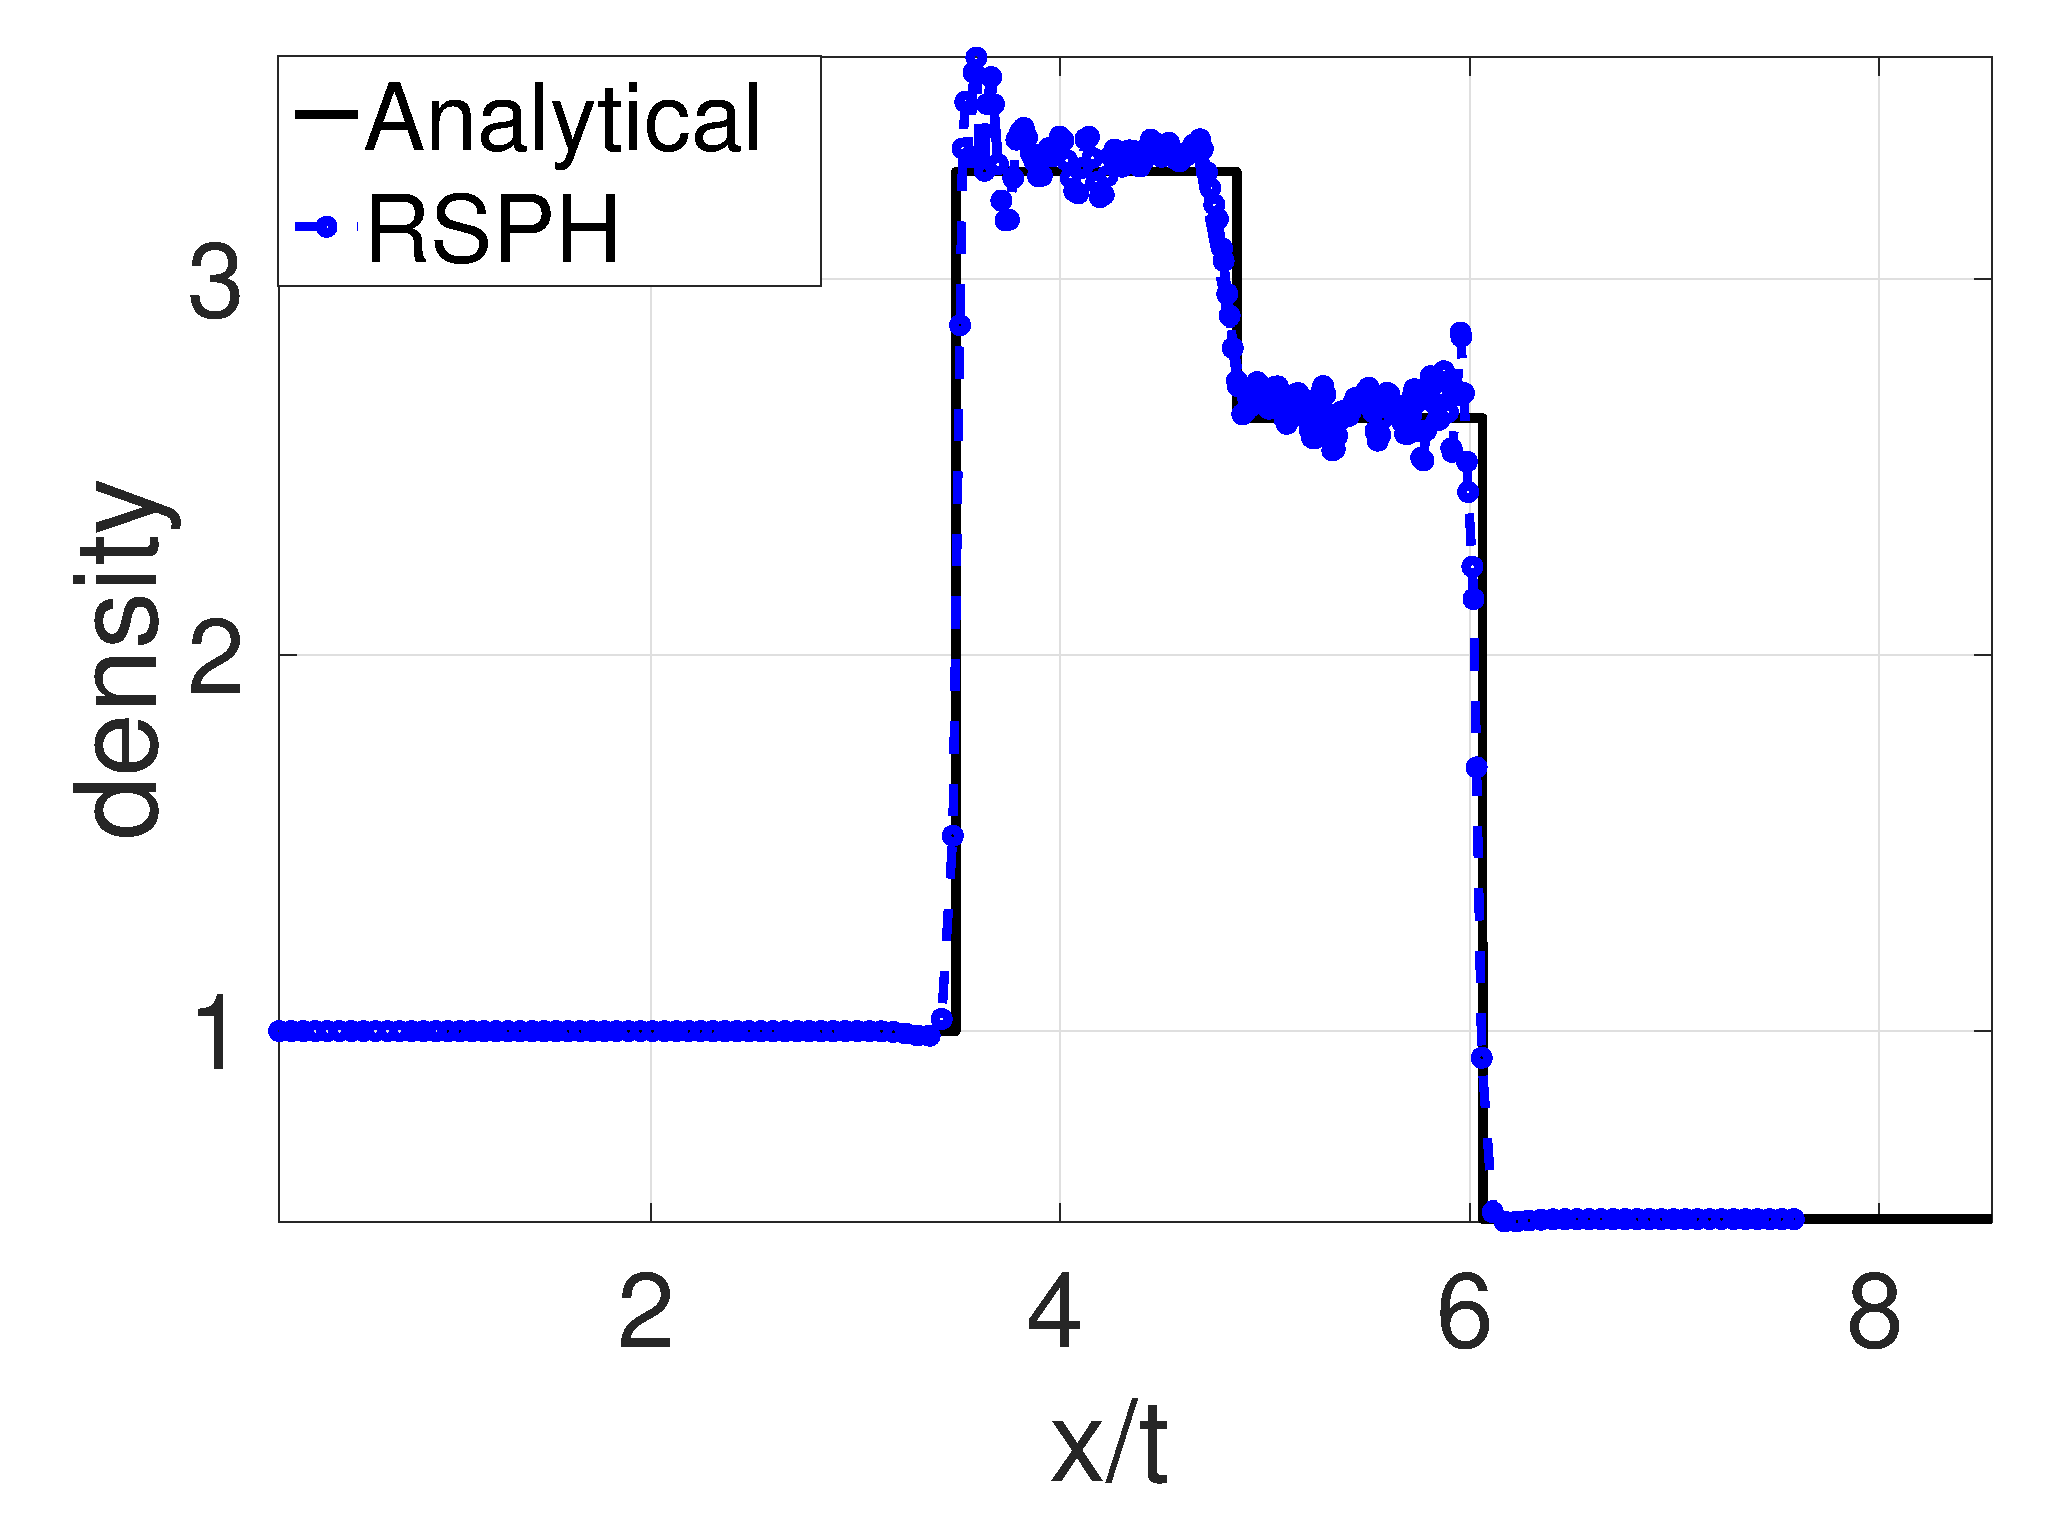
\includegraphics[width=0.99 \textwidth]{./Chapter-4/Figures/double_shock/Dshock-RCM-rho-Rp6}
    \end{minipage}%
    \begin{minipage}{.415 \textwidth}
        \centering
        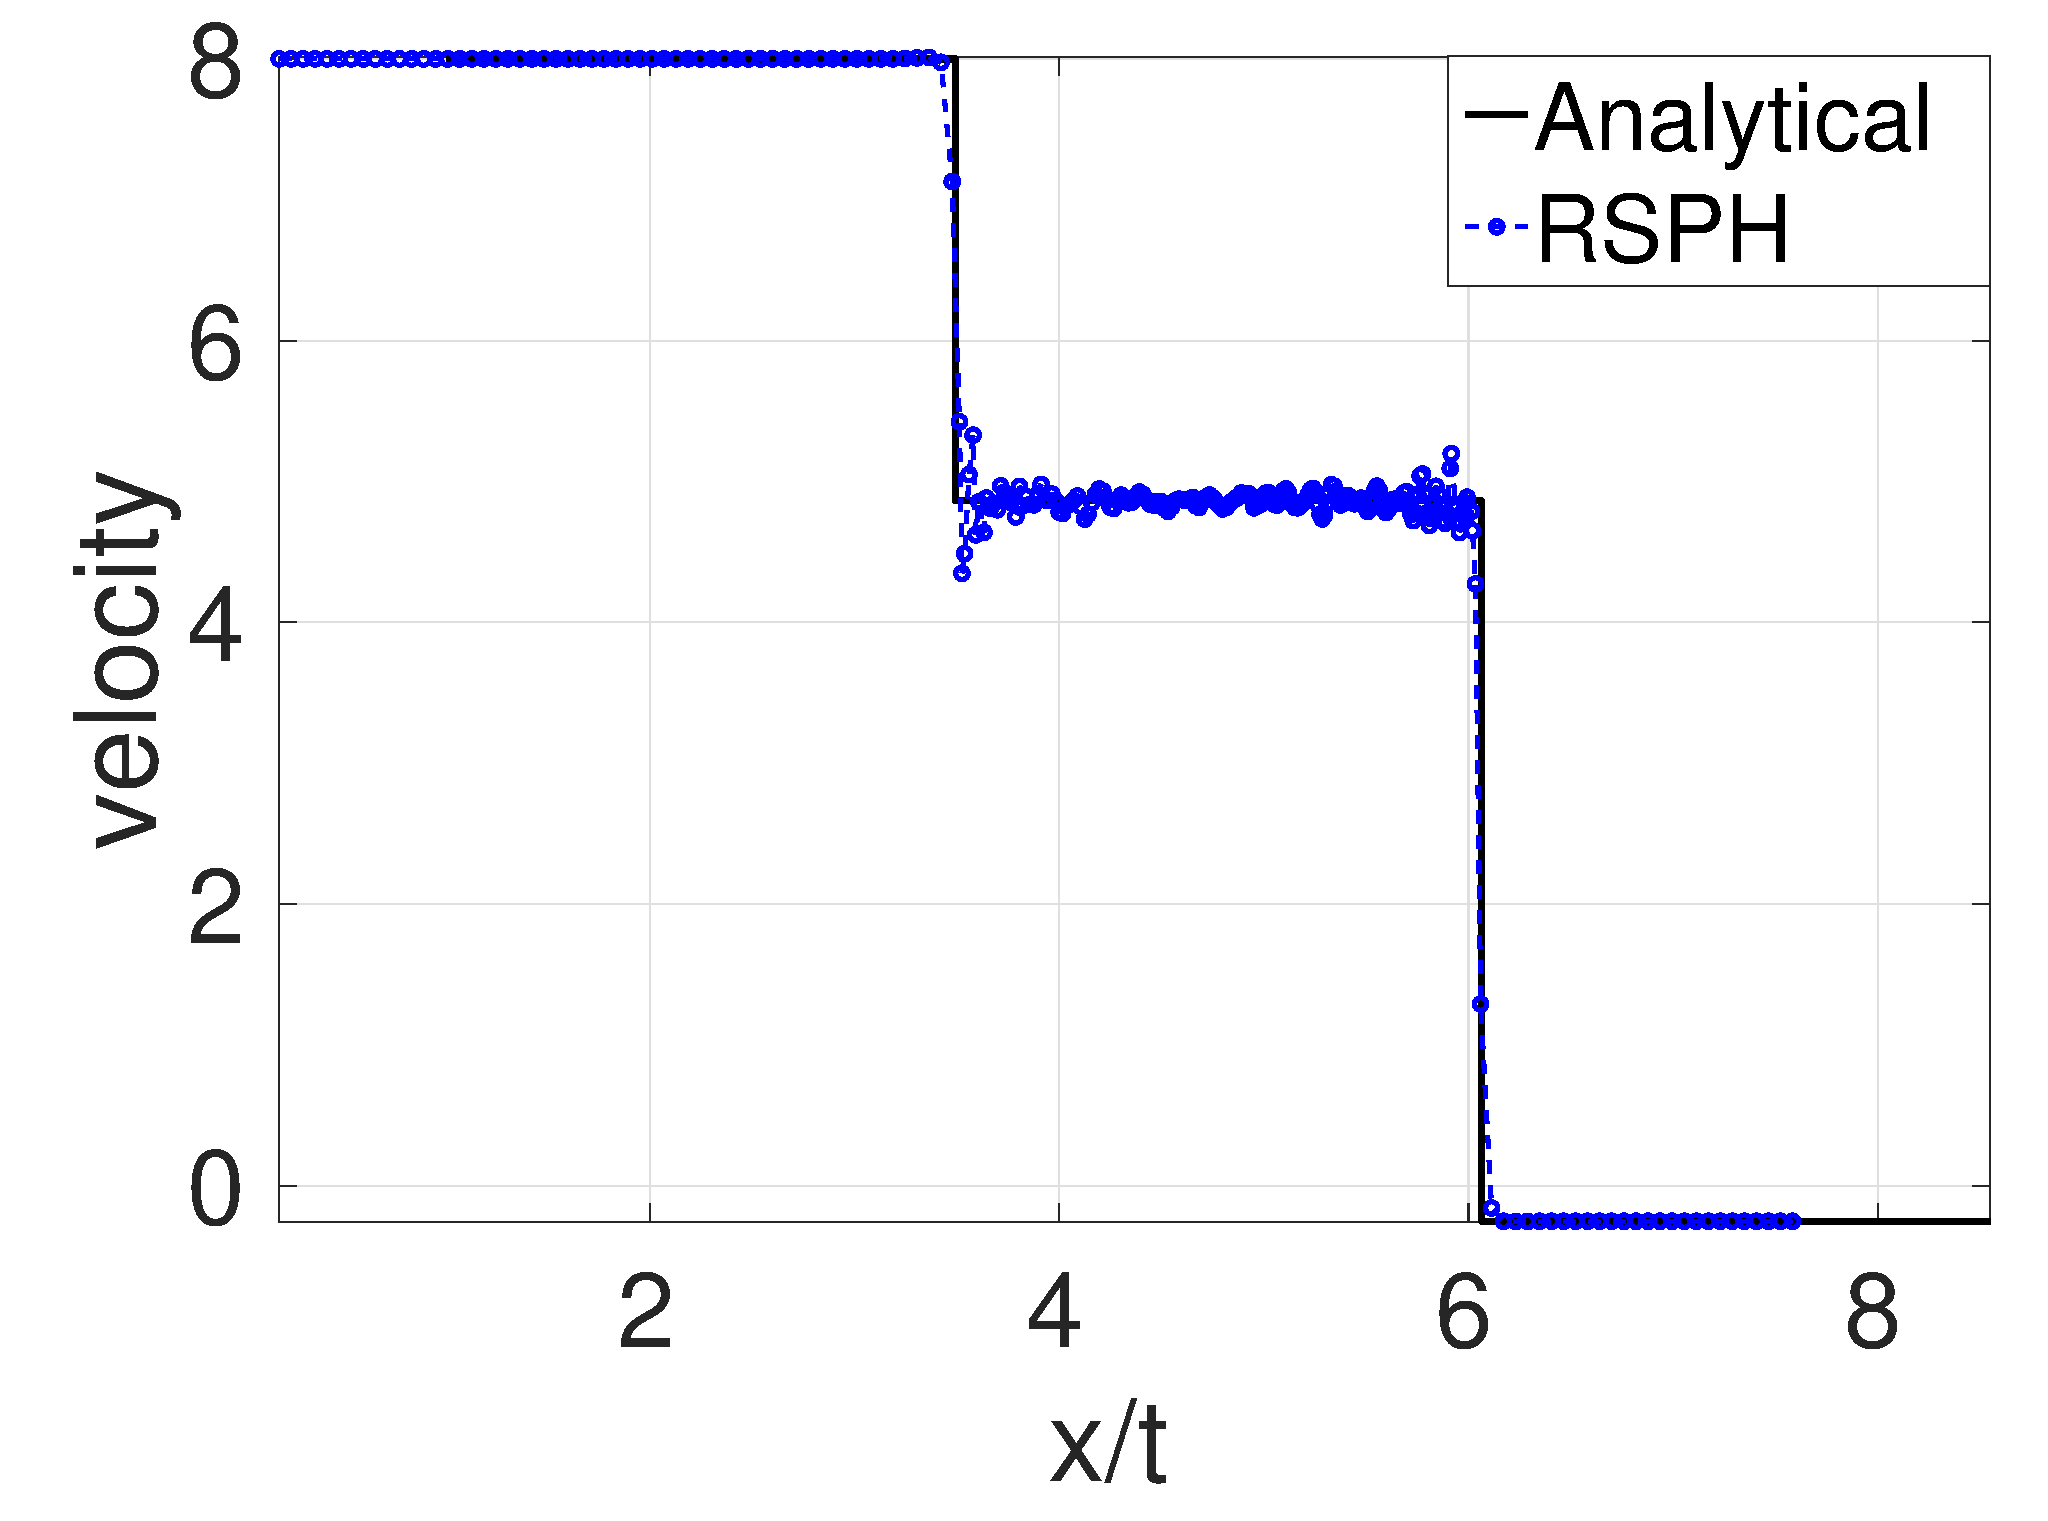
\includegraphics[width=0.99 \textwidth]{./Chapter-4/Figures/double_shock/Dshock-RCM-v-Rp6}
    \end{minipage}%
    \\
    \begin{minipage}{.415\textwidth}
        \centering
        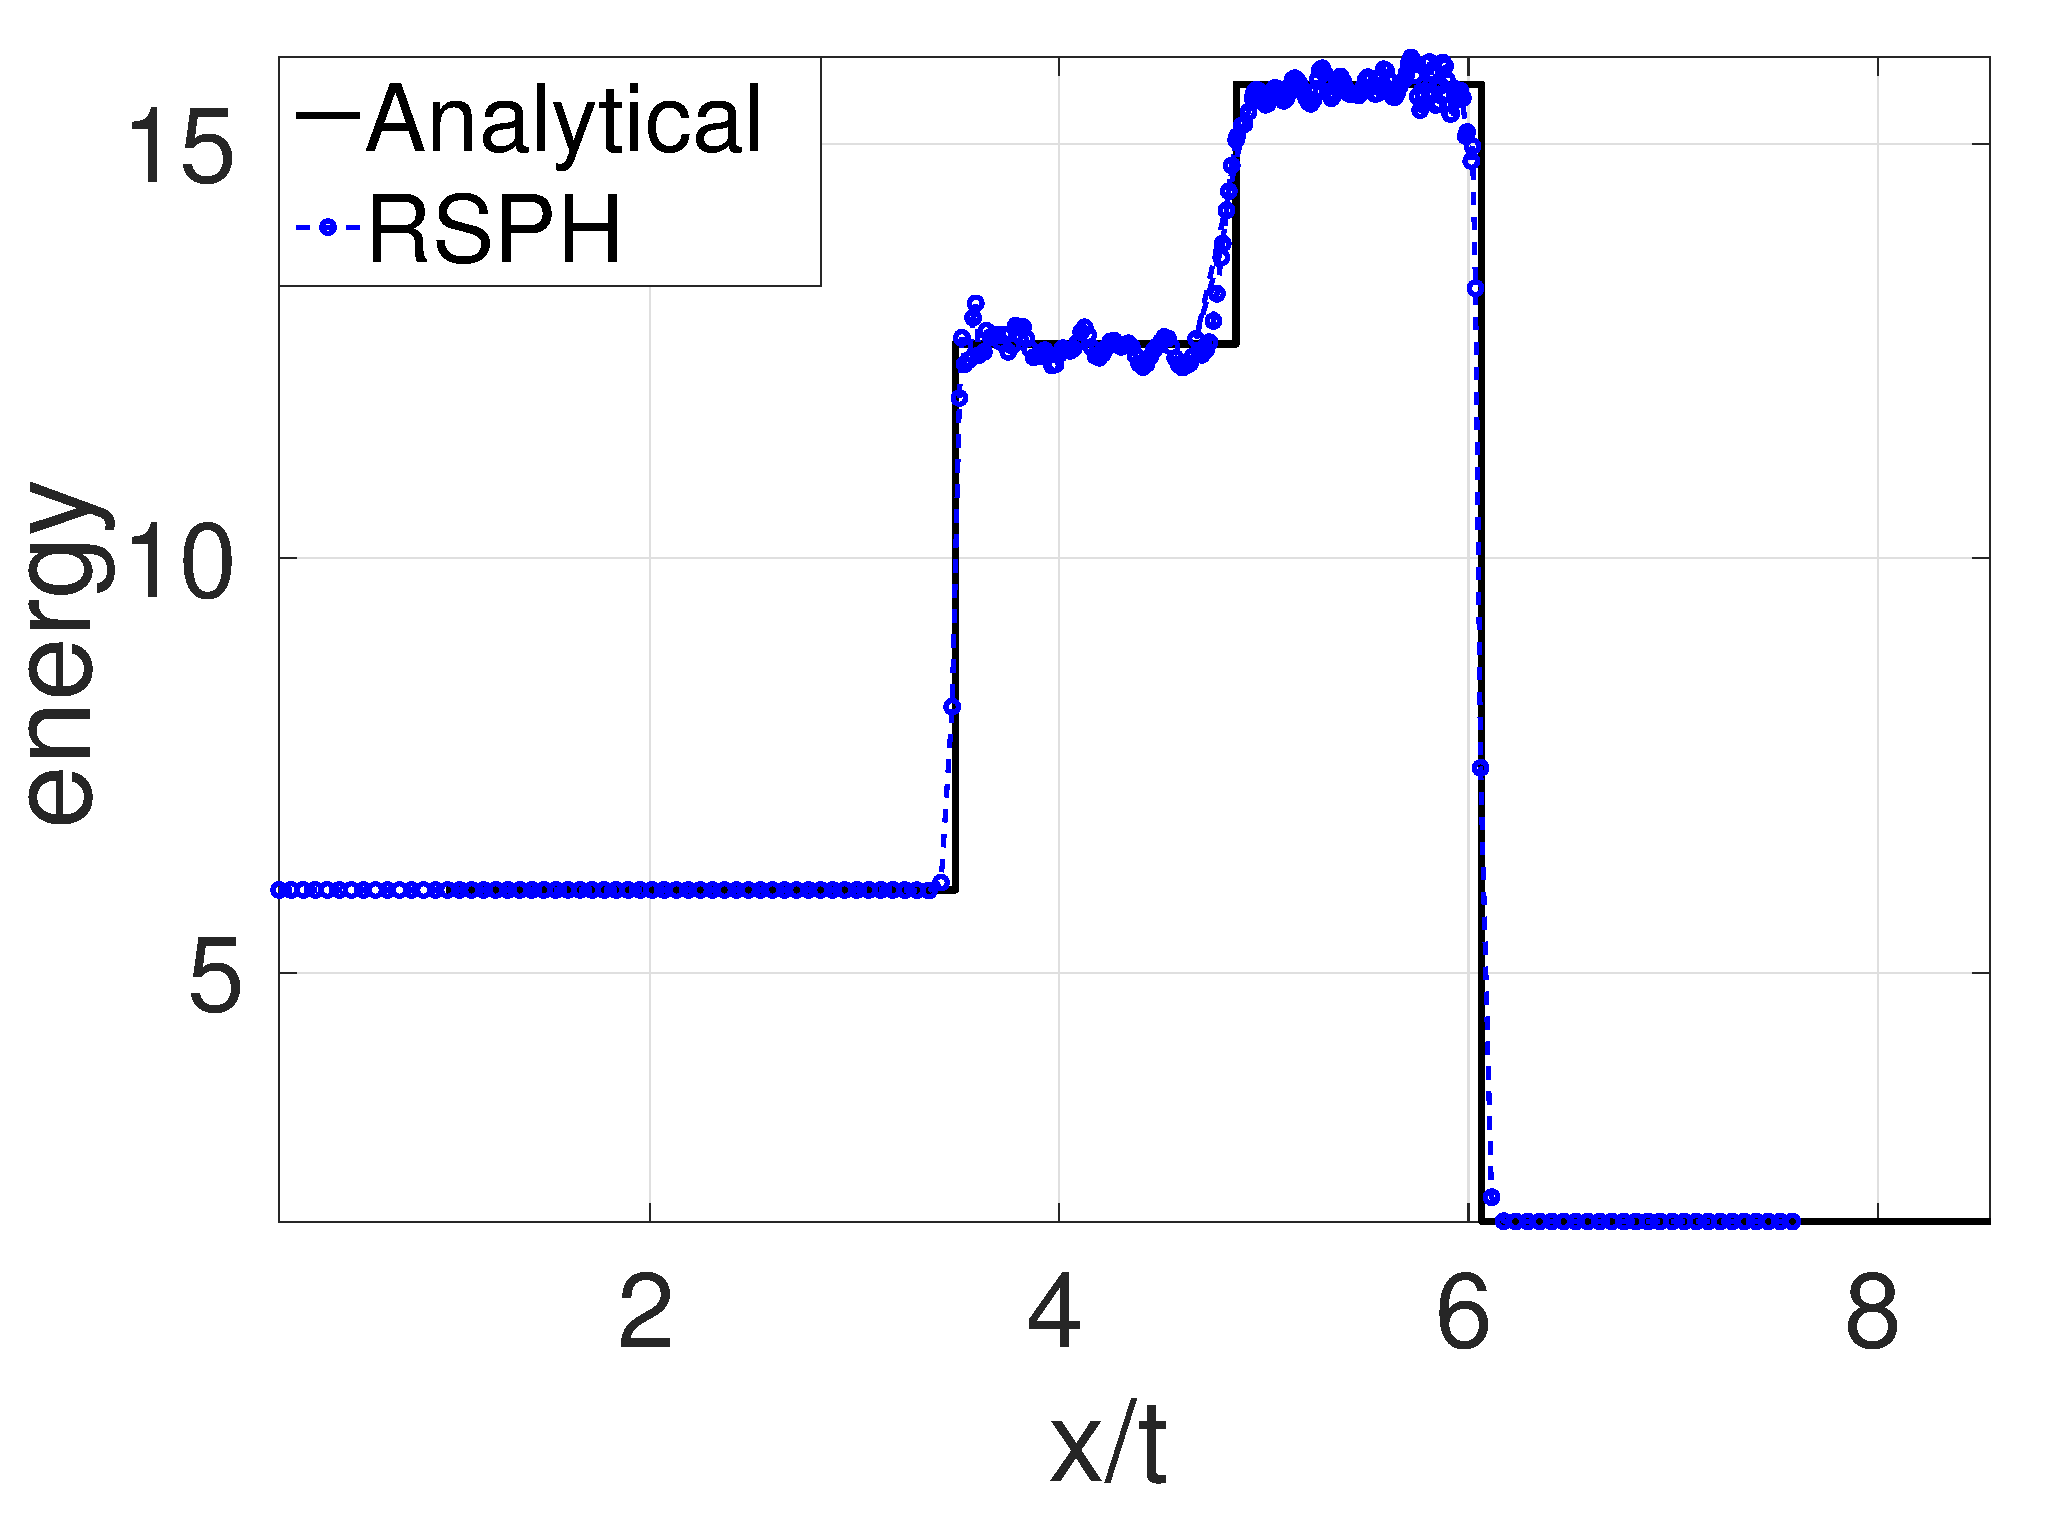
\includegraphics[width=0.99 \textwidth]{./Chapter-4/Figures/double_shock/Dshock-RCM-e-Rp6}
    \end{minipage}%
    \begin{minipage}{.415 \textwidth}
        \centering
        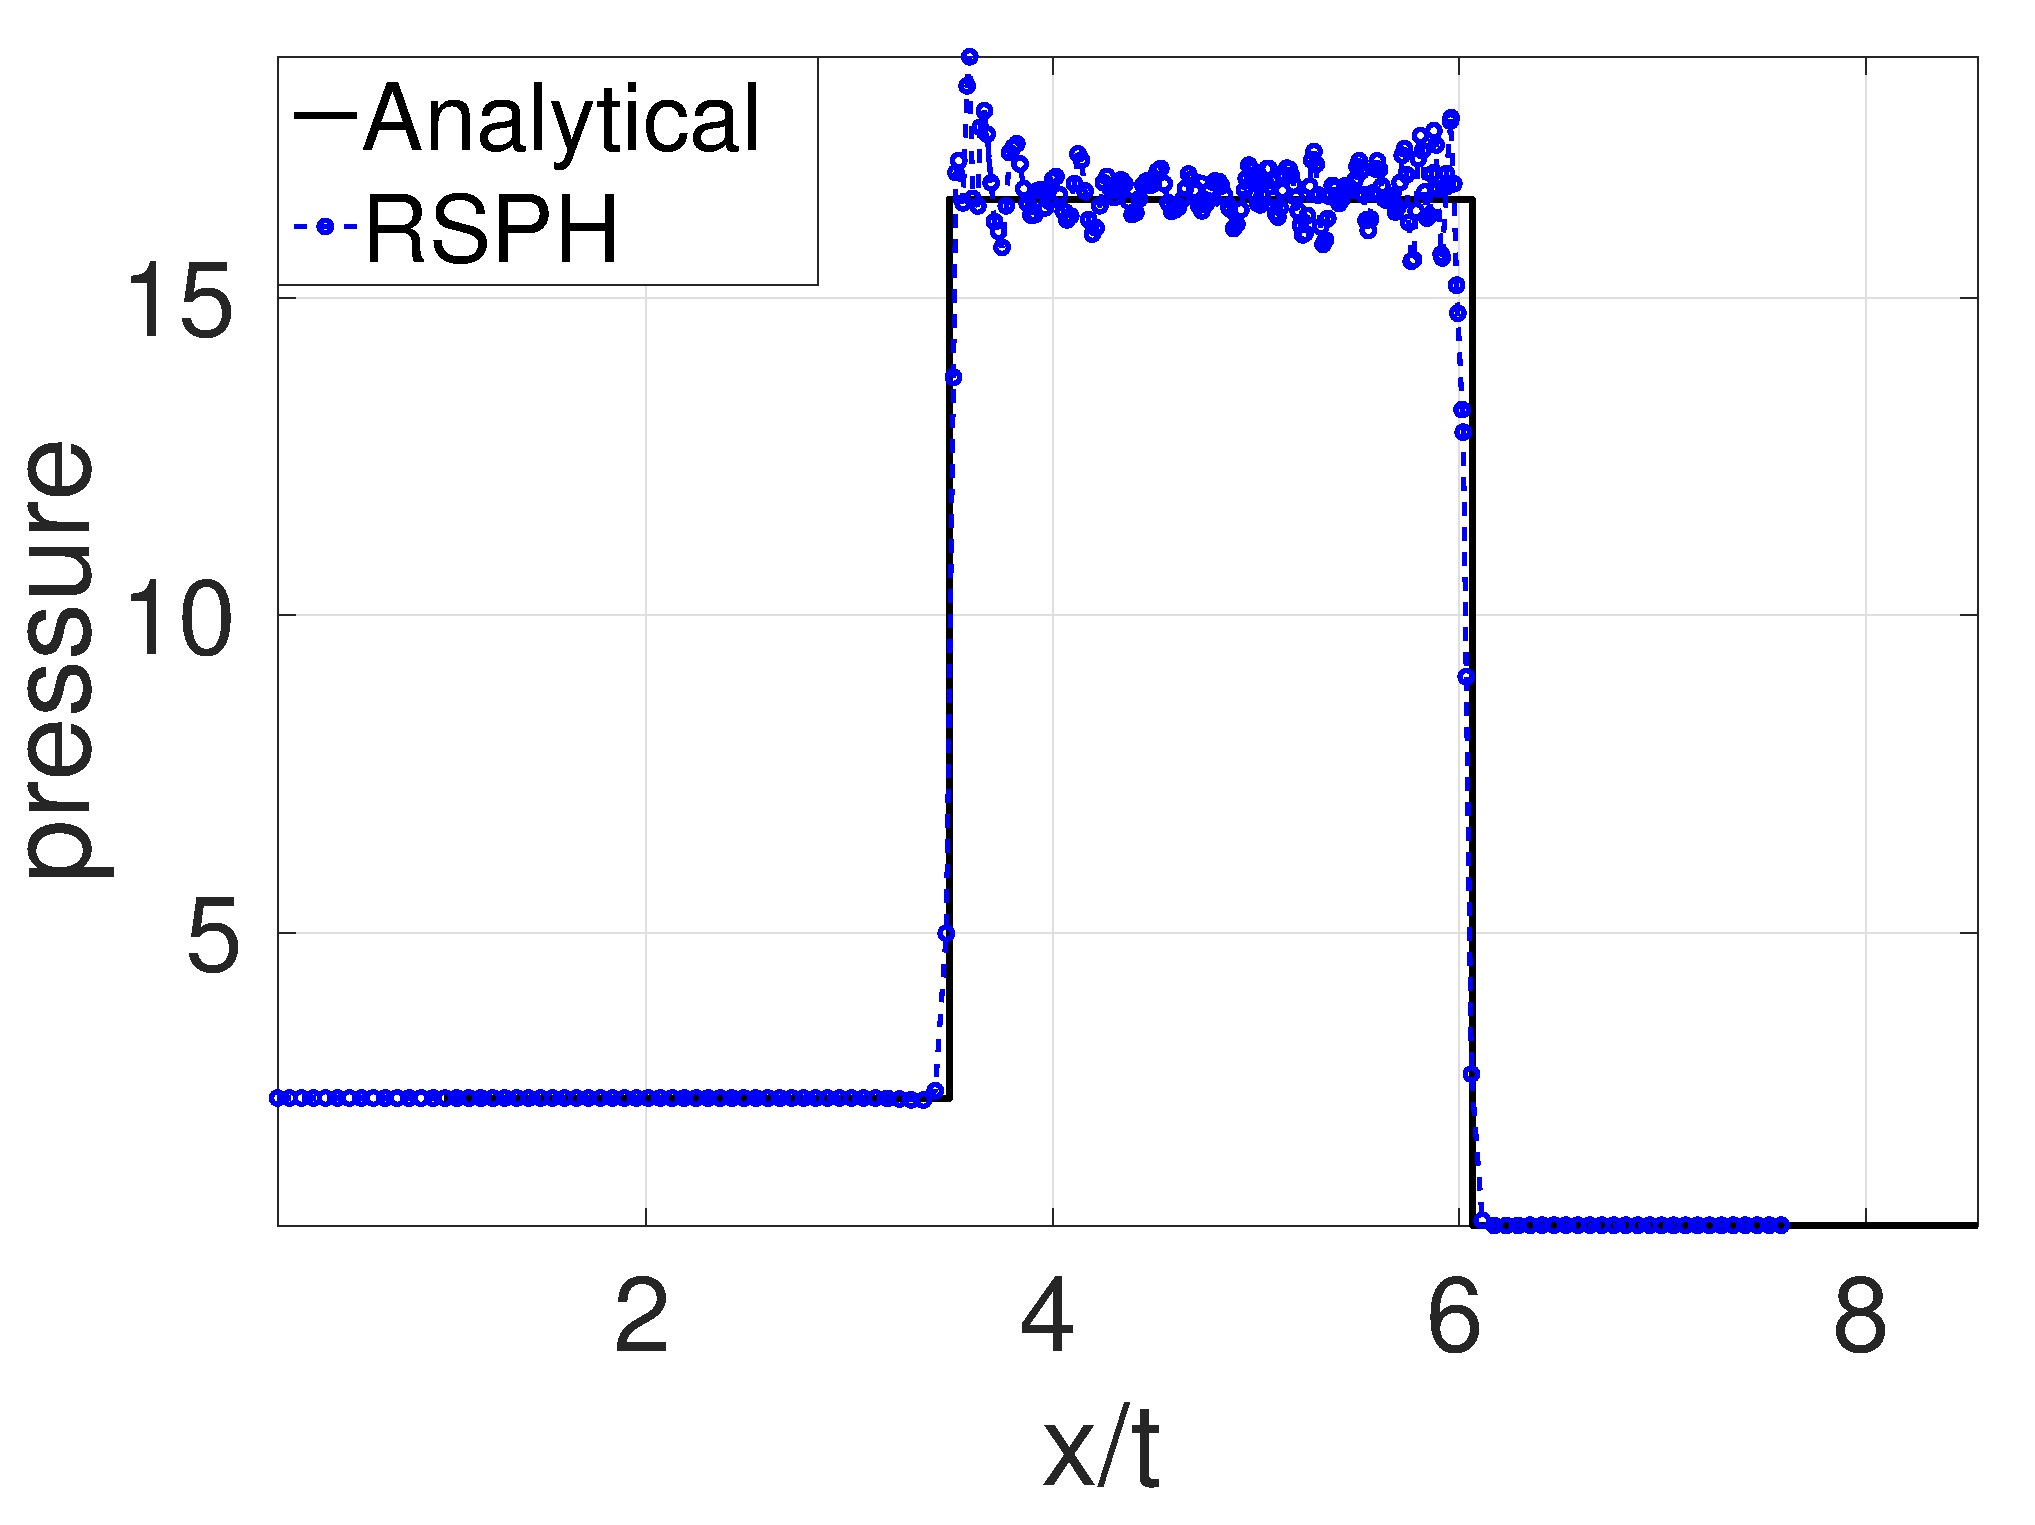
\includegraphics[width=0.99 \textwidth]{./Chapter-4/Figures/double_shock/Dshock-RCM-p-Rp6}
    \end{minipage}% 
    \caption{Results for test 4, the double shock case. To stabilize the simulation, RSPH sampling is in a narrower range. All physical properties are well re-produced. However, the oscillations are more serious than oscillations in other tests.}
    \label{fig:RCM-double-shock}
\end{figure}

\begin{figure}
	\centering
    \begin{minipage}{.415\textwidth}
        \centering
        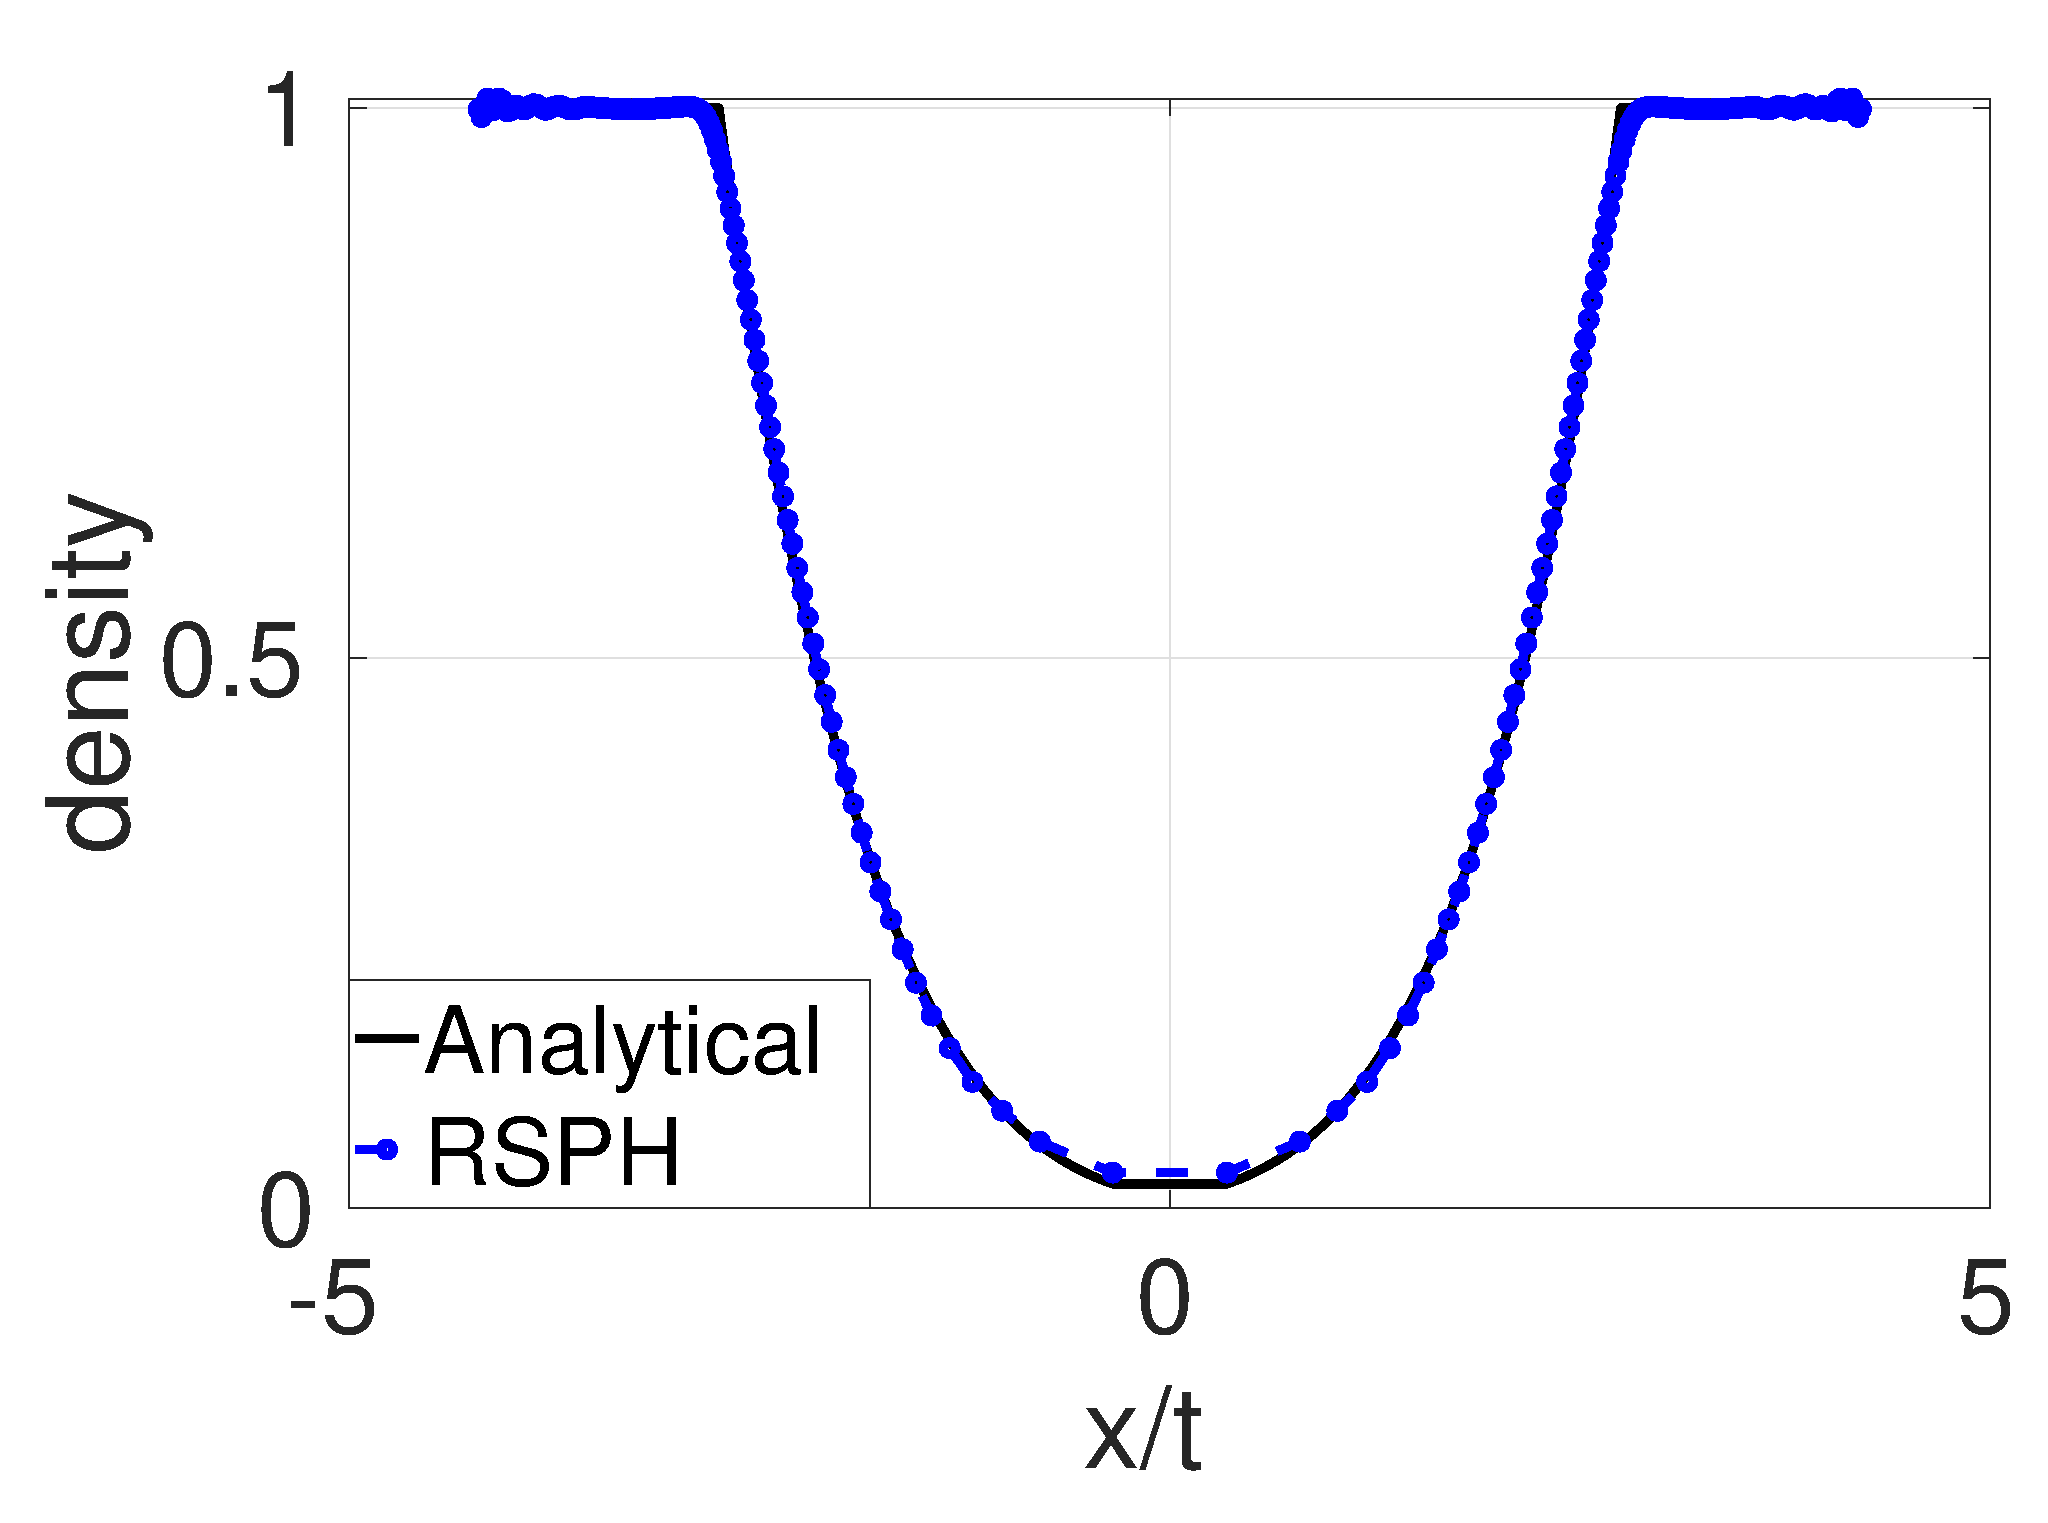
\includegraphics[width=0.99 \textwidth]{./Chapter-4/Figures/Sjogreen/Sjogreen-RCM-rho-Adpt1}
    \end{minipage}%
    \begin{minipage}{.415 \textwidth}
        \centering
        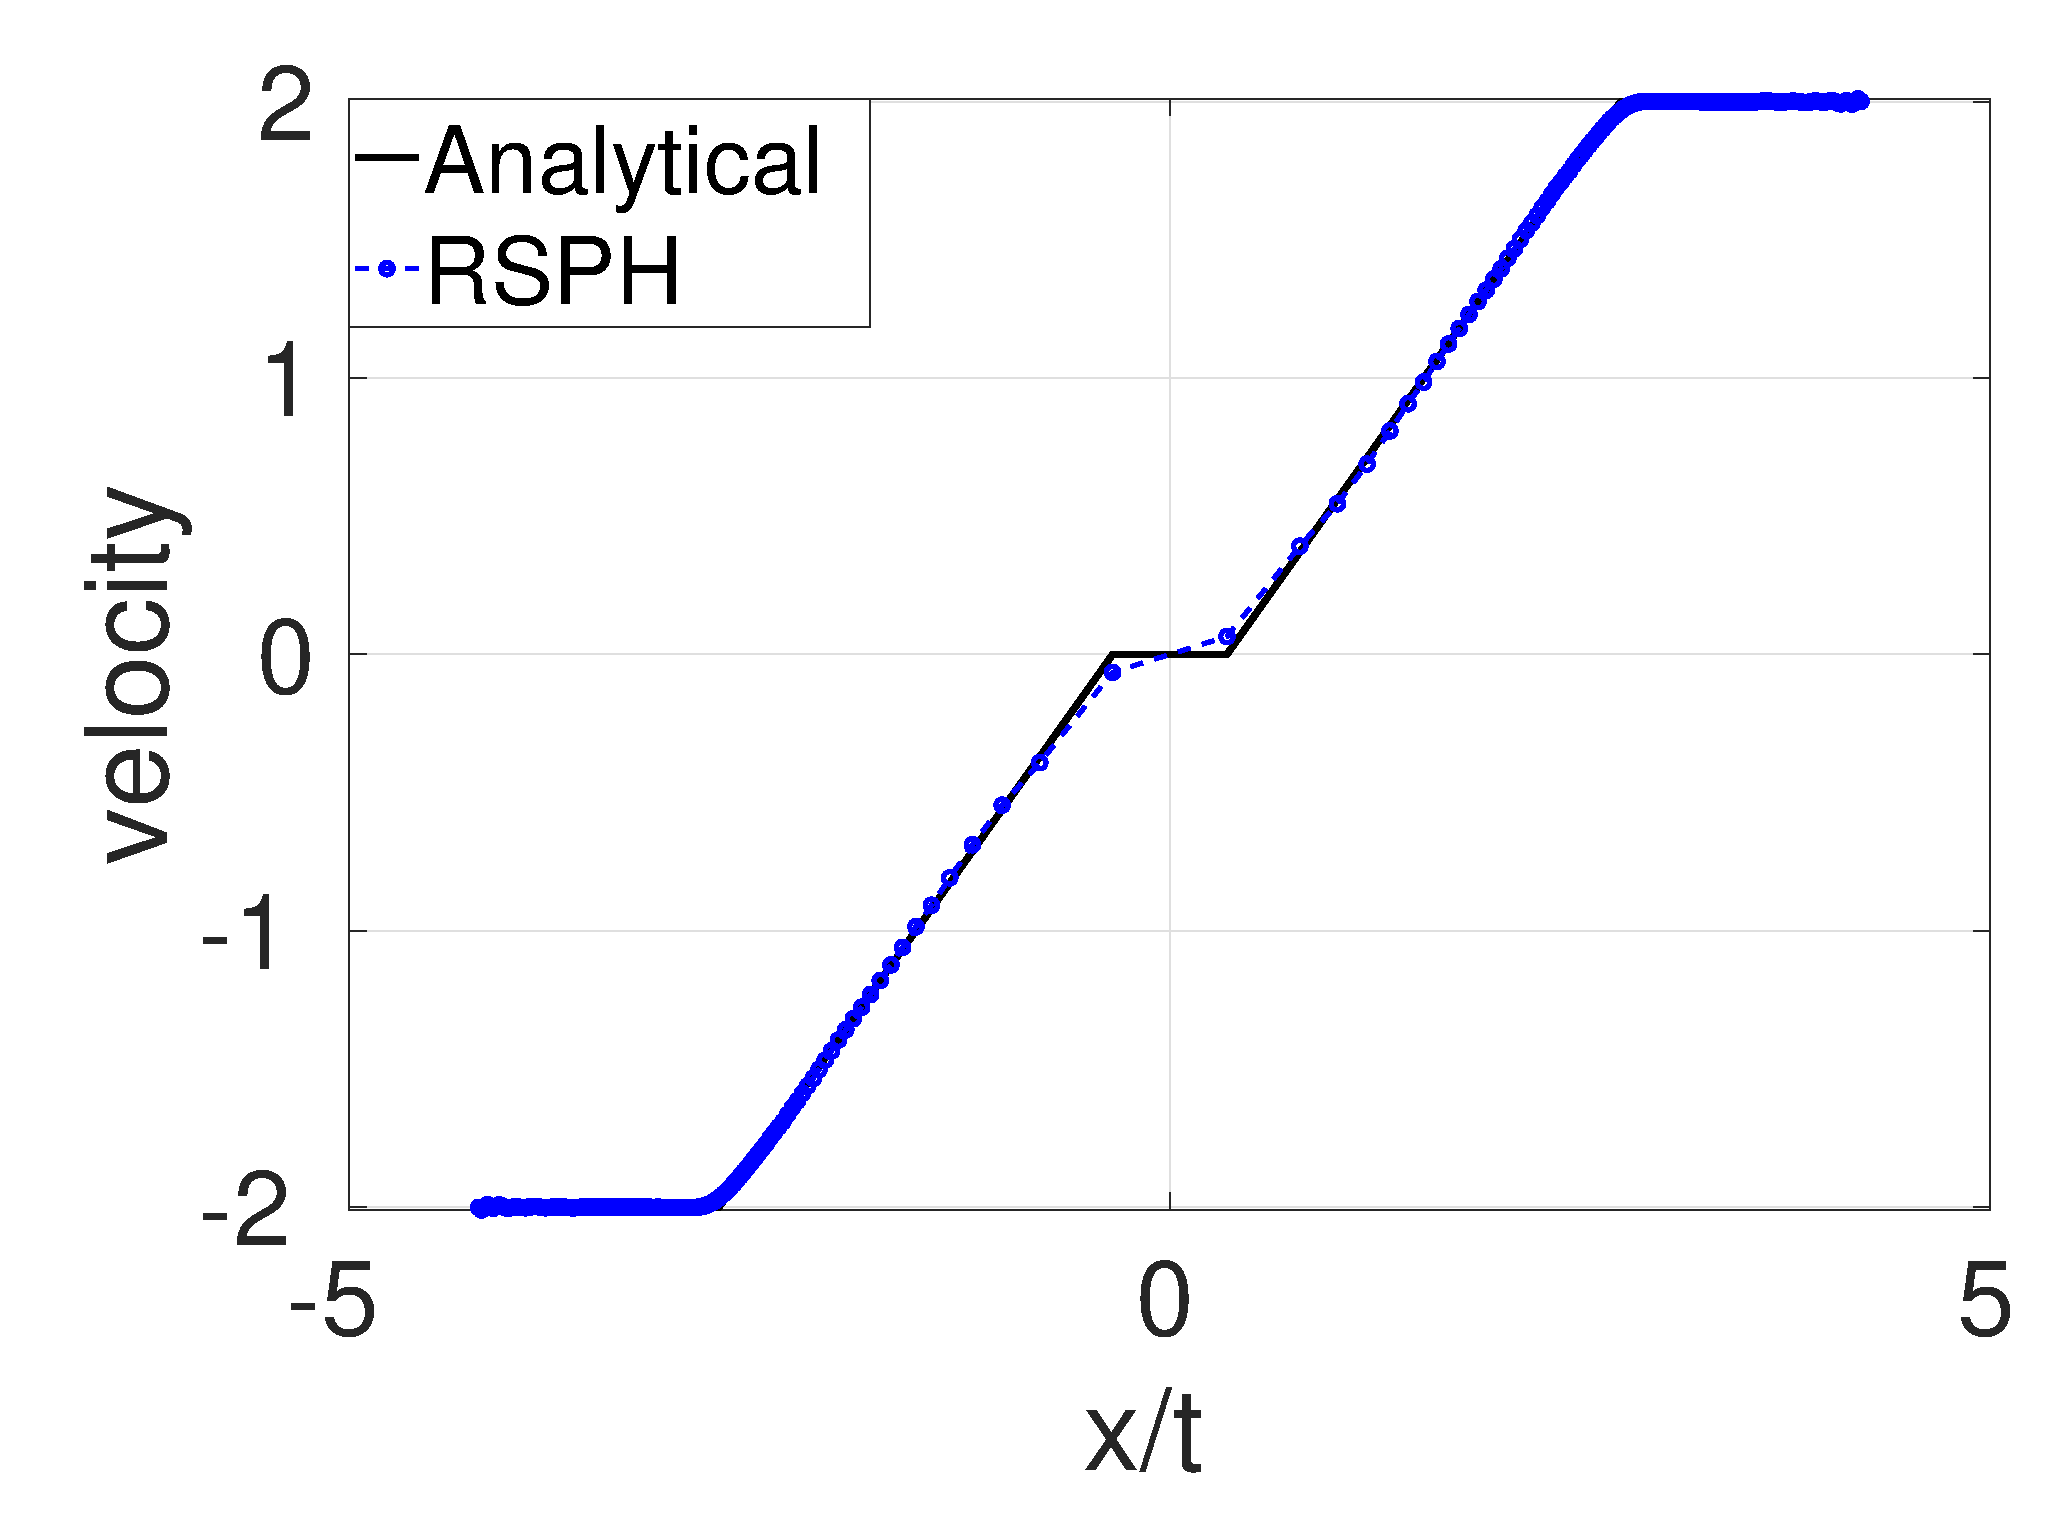
\includegraphics[width=0.99 \textwidth]{./Chapter-4/Figures/Sjogreen/Sjogreen-RCM-v-Adpt1}
    \end{minipage}%
    \\
    \begin{minipage}{.415\textwidth}
        \centering
        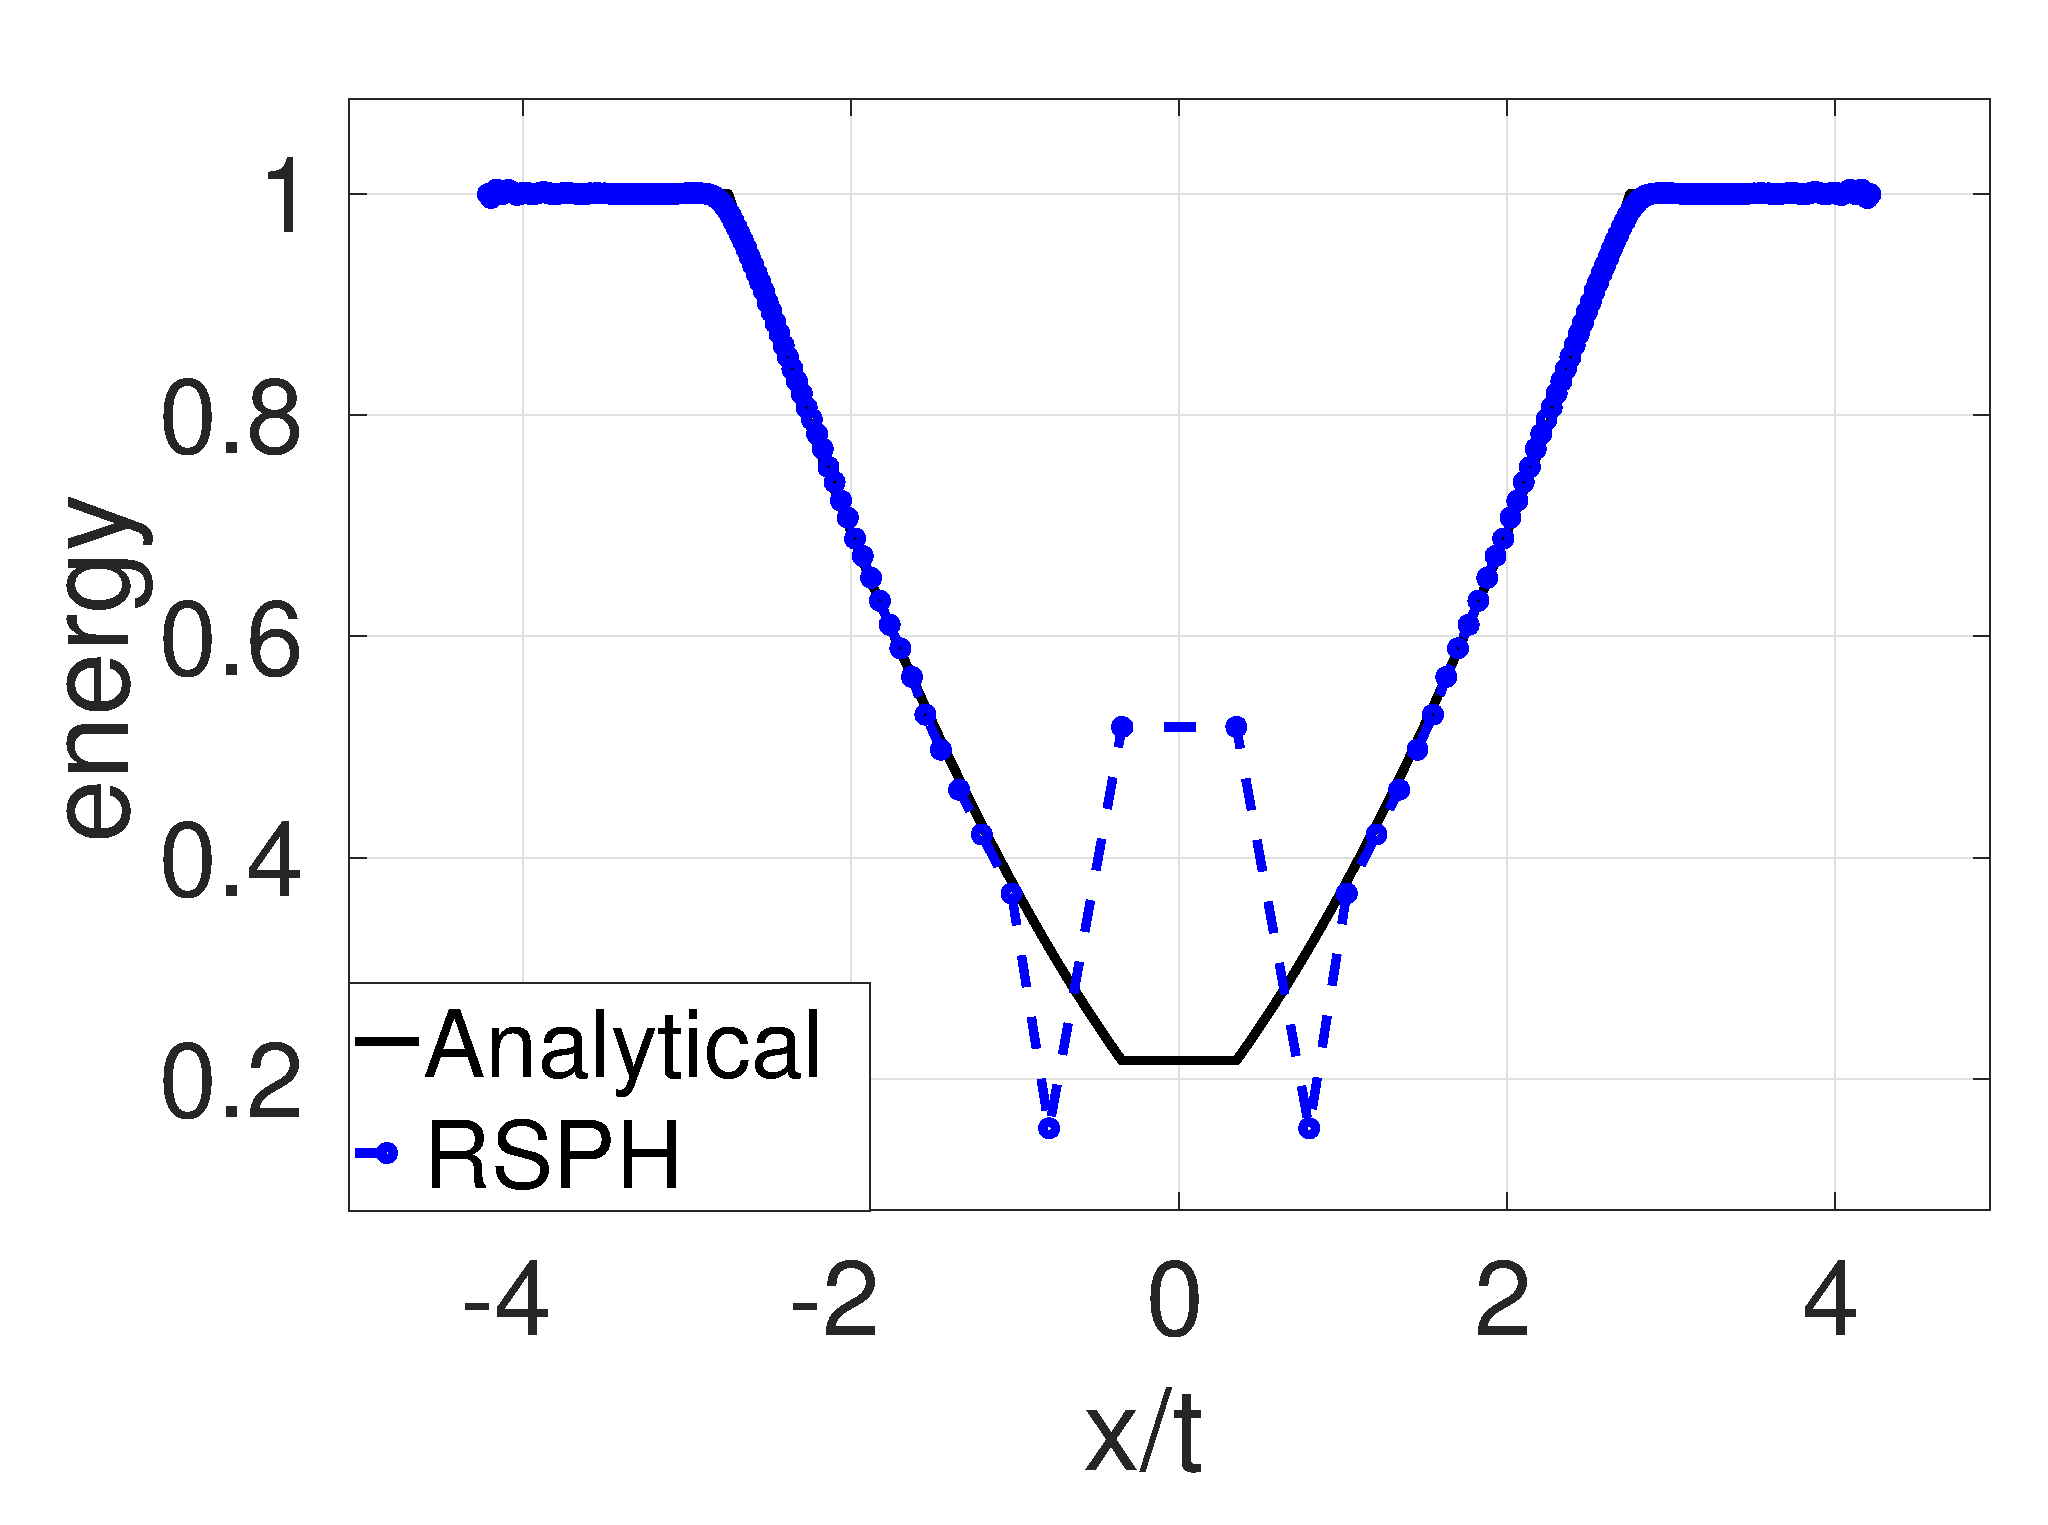
\includegraphics[width=0.99 \textwidth]{./Chapter-4/Figures/Sjogreen/Sjogreen-RCM-e-Adpt1}
    \end{minipage}%
    \begin{minipage}{.415 \textwidth}
        \centering
        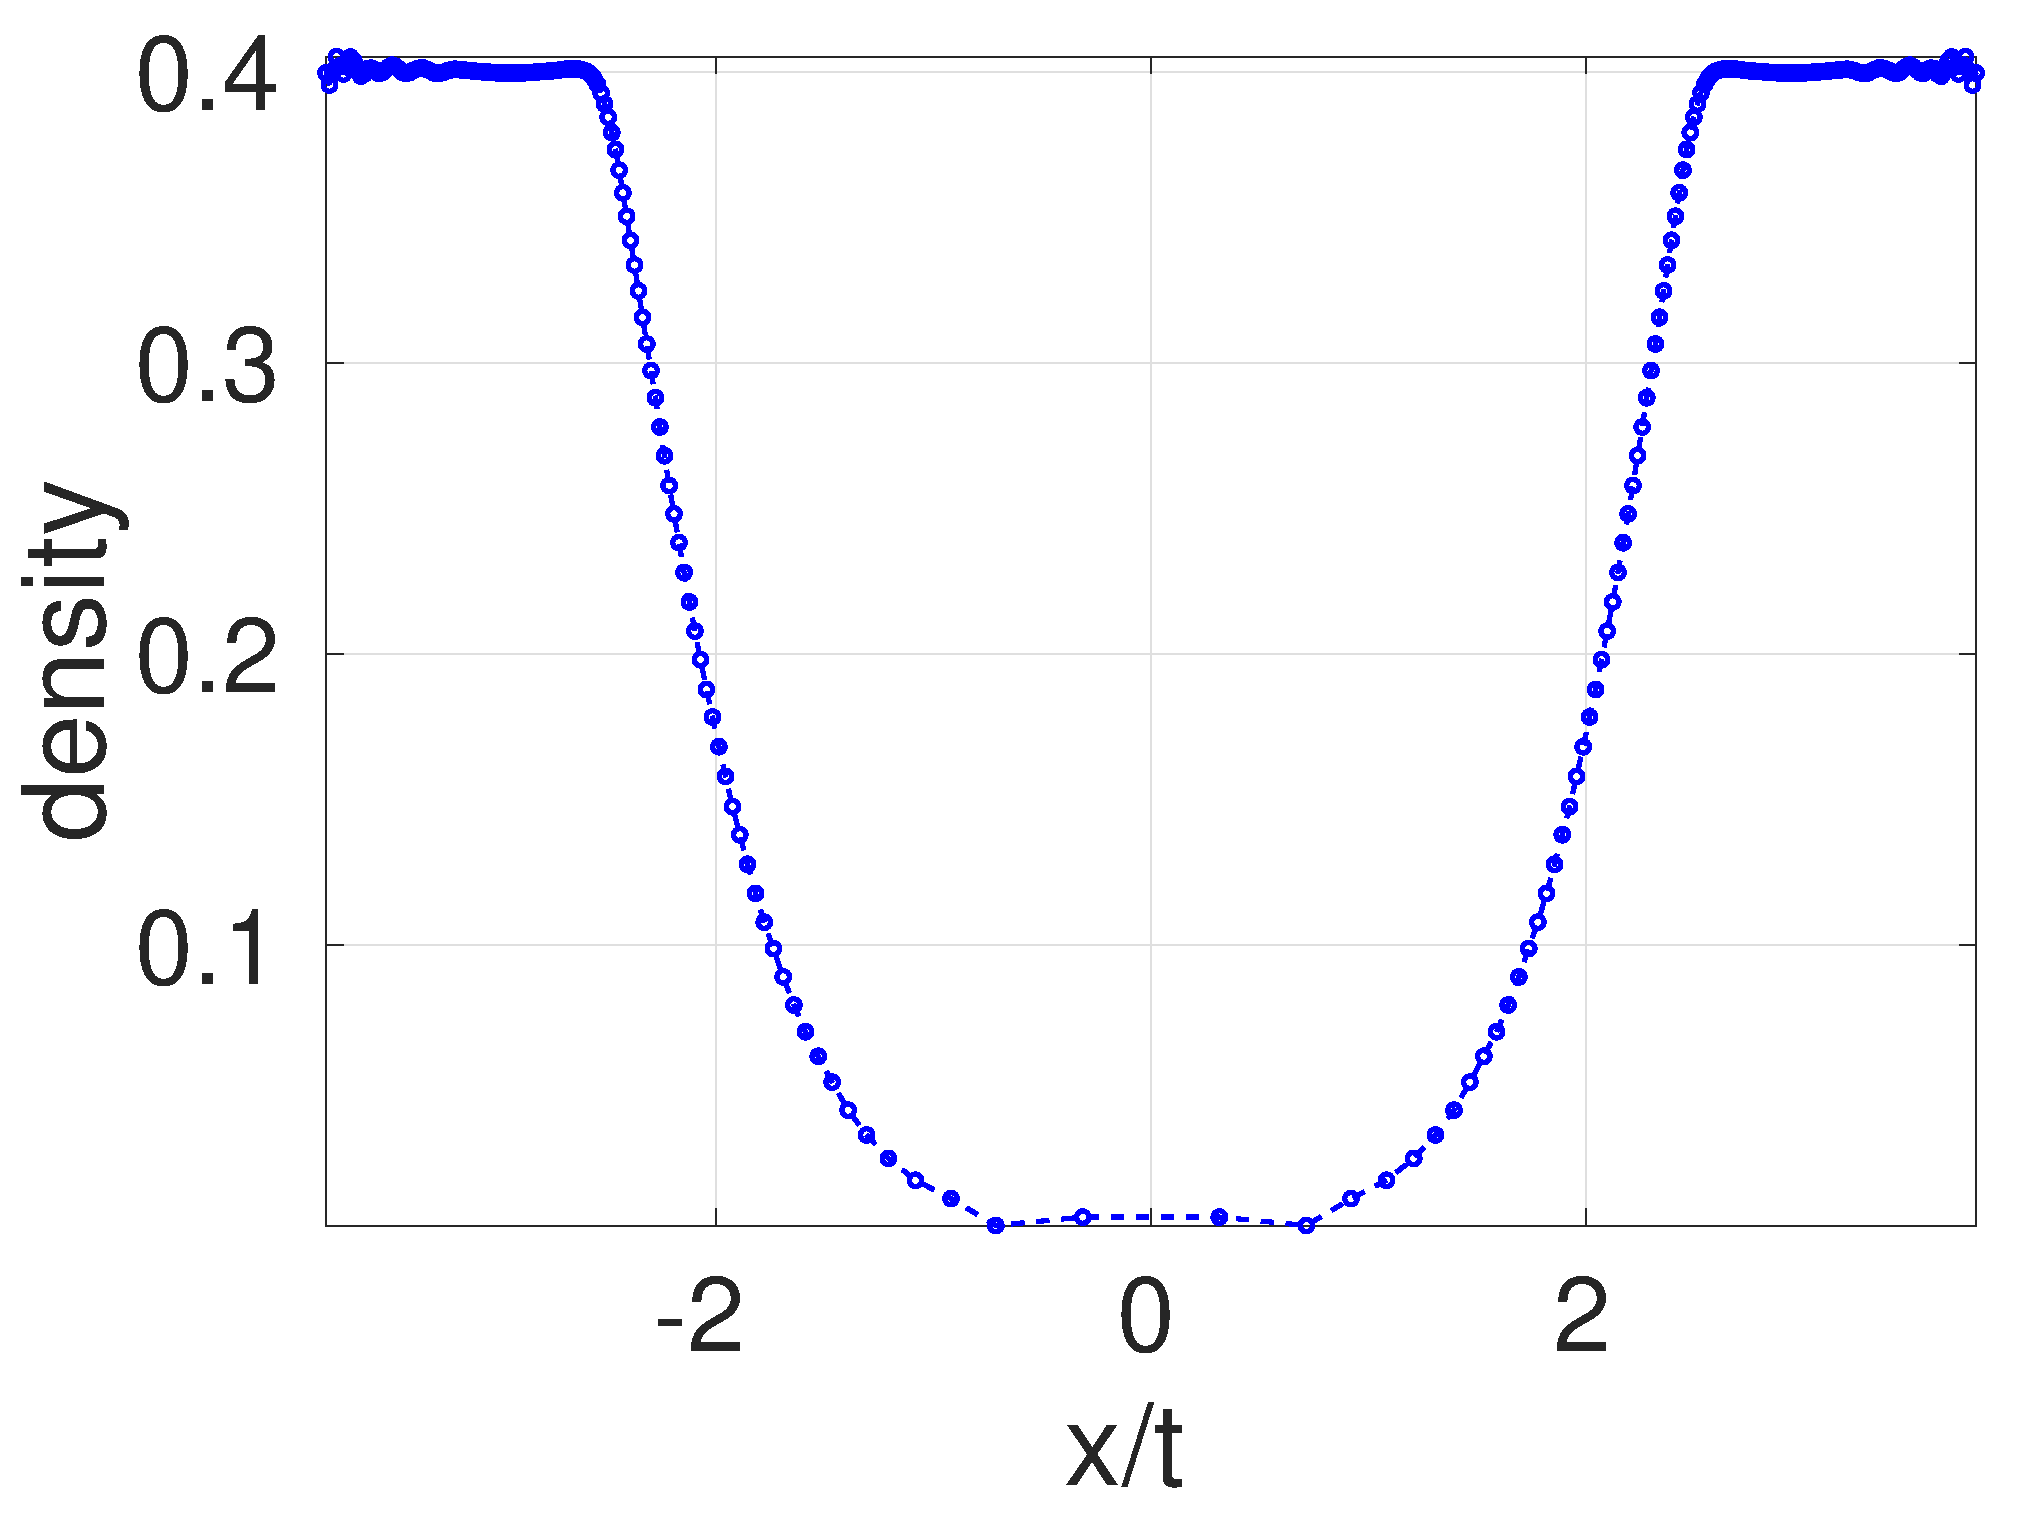
\includegraphics[width=0.99 \textwidth]{./Chapter-4/Figures/Sjogreen/Sjogreen-RCM-p-Adpt1}
    \end{minipage}% 
    \caption{Results for test 5, a variation of the Sj$\ddot{o}$green test. The density, velocity and pressure are well re-produced while the thermal energy at the origin is poorly predicted. A jump of internal energy at the origin is a common issue in many SPH schemes (see, for example, \citep{monaghan1997sph,cha2003implementations,puri2014approximate})}
    \label{fig:RCM-Sjogreen}
\end{figure}

\begin{figure}
    \centering
    \begin{minipage}{.415\textwidth}
        \centering
        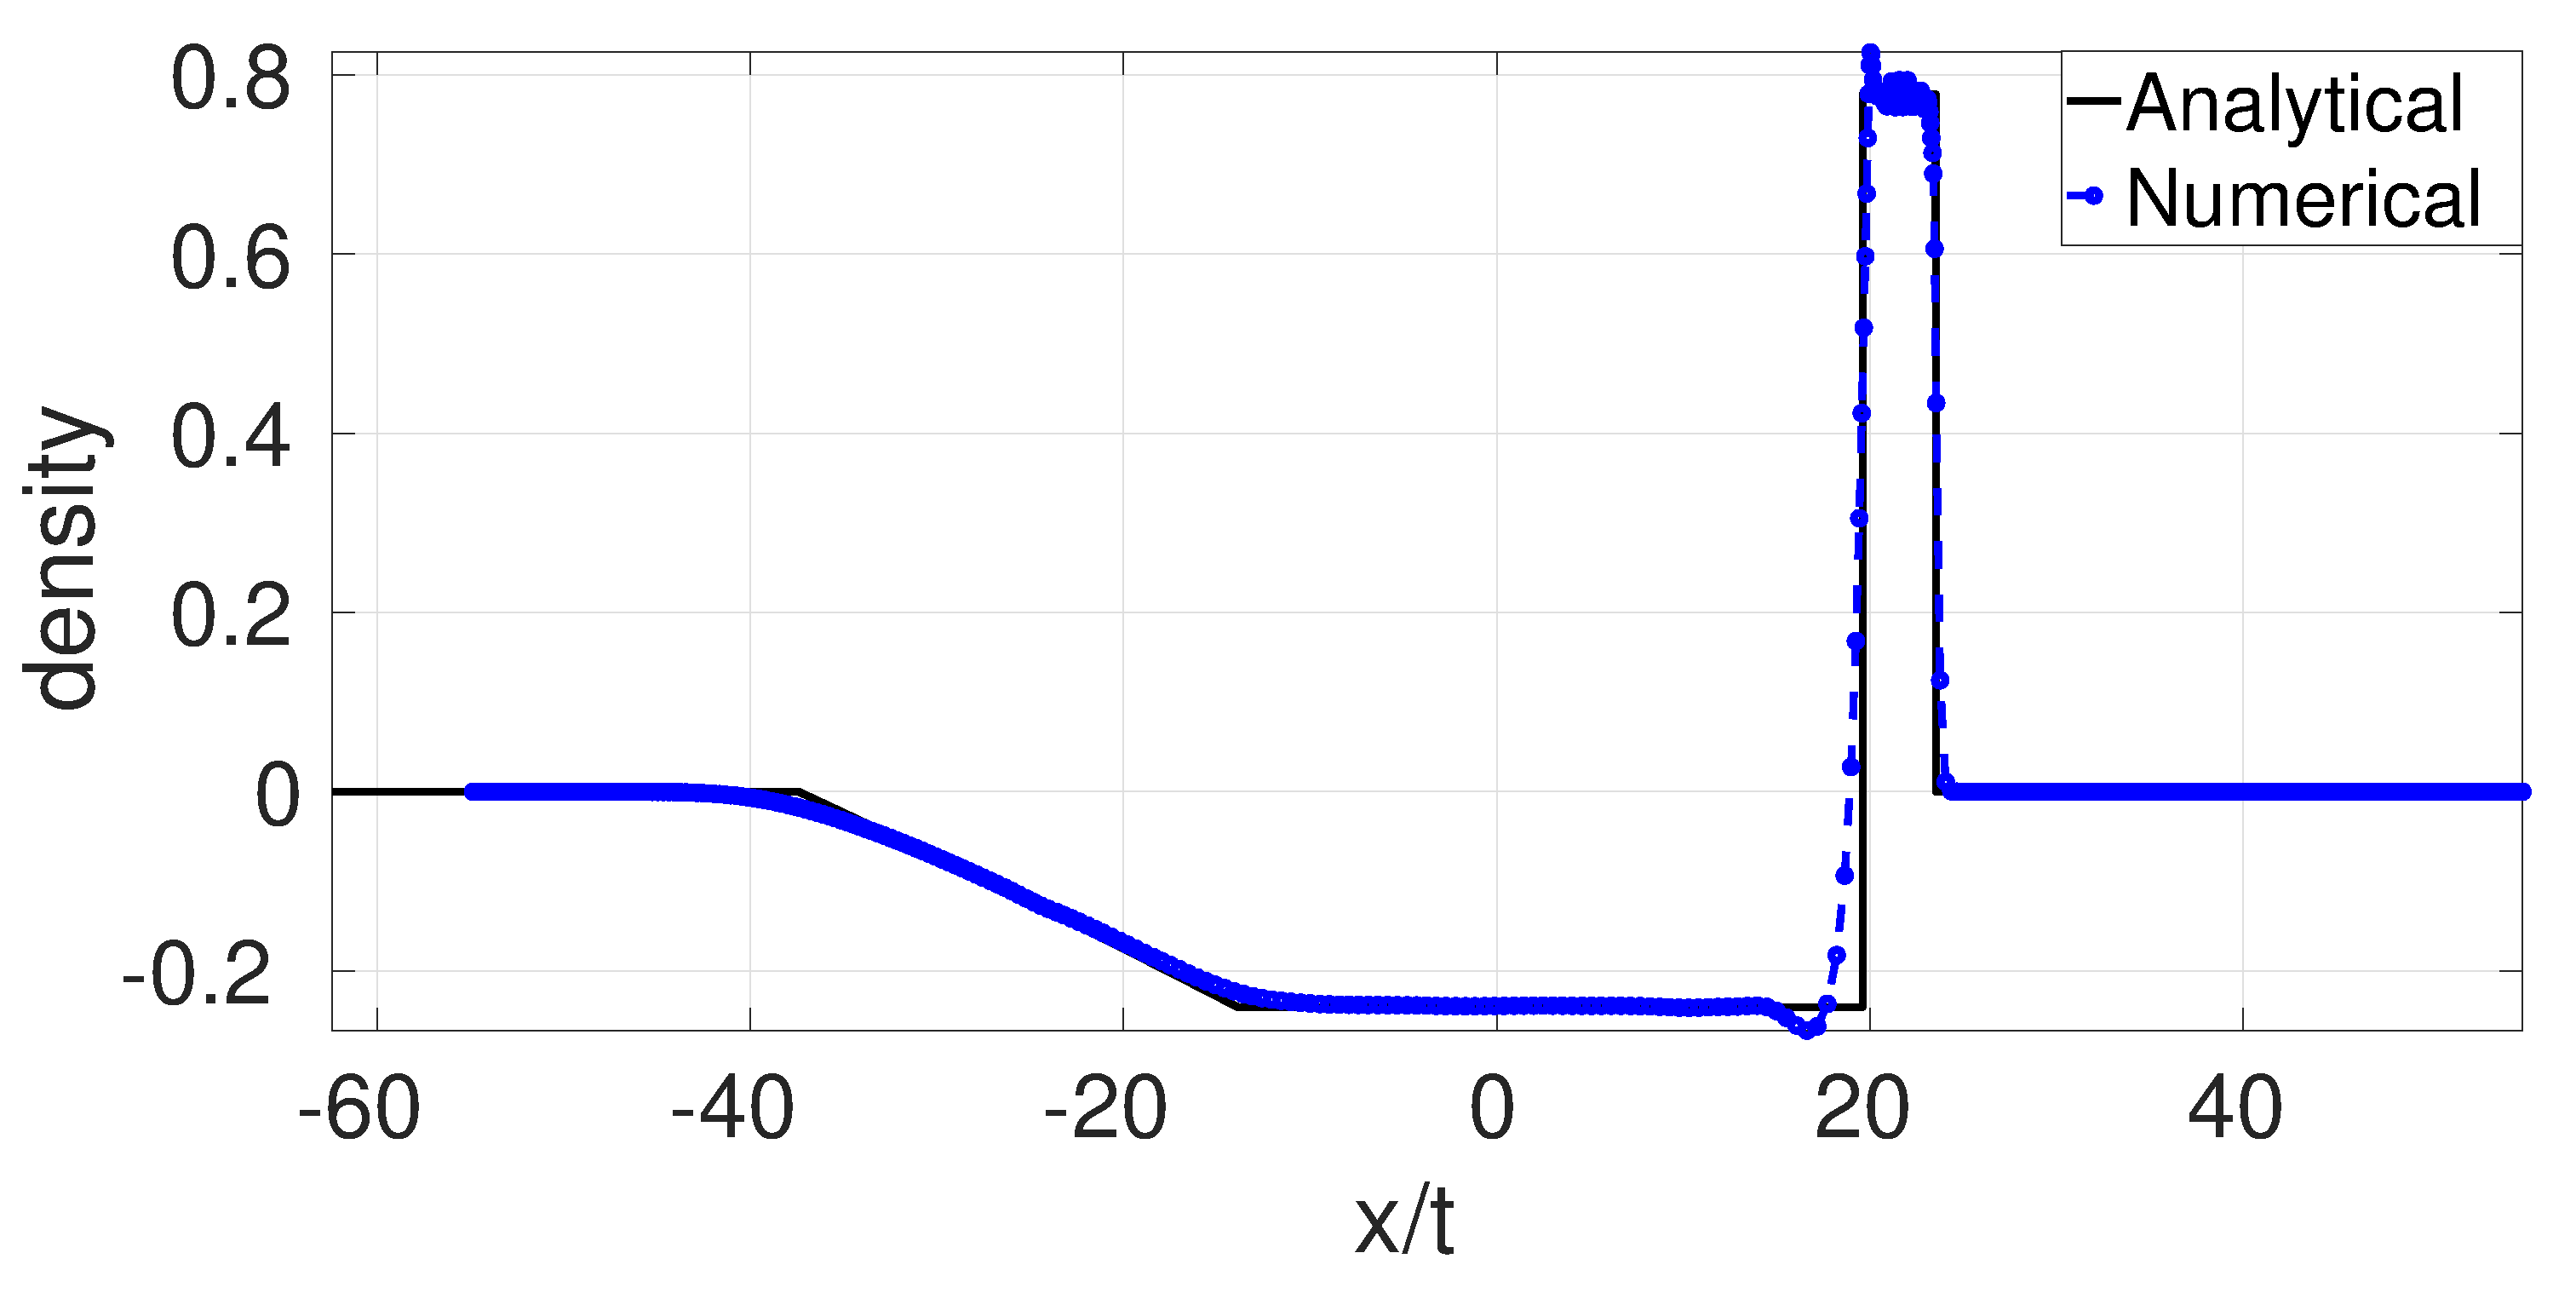
\includegraphics[width=0.99 \textwidth]{./Chapter-4/Figures/strong-blast/StrBlst-RCM-rho-Rp3}
    \end{minipage}%
    \begin{minipage}{.415 \textwidth}
        \centering
        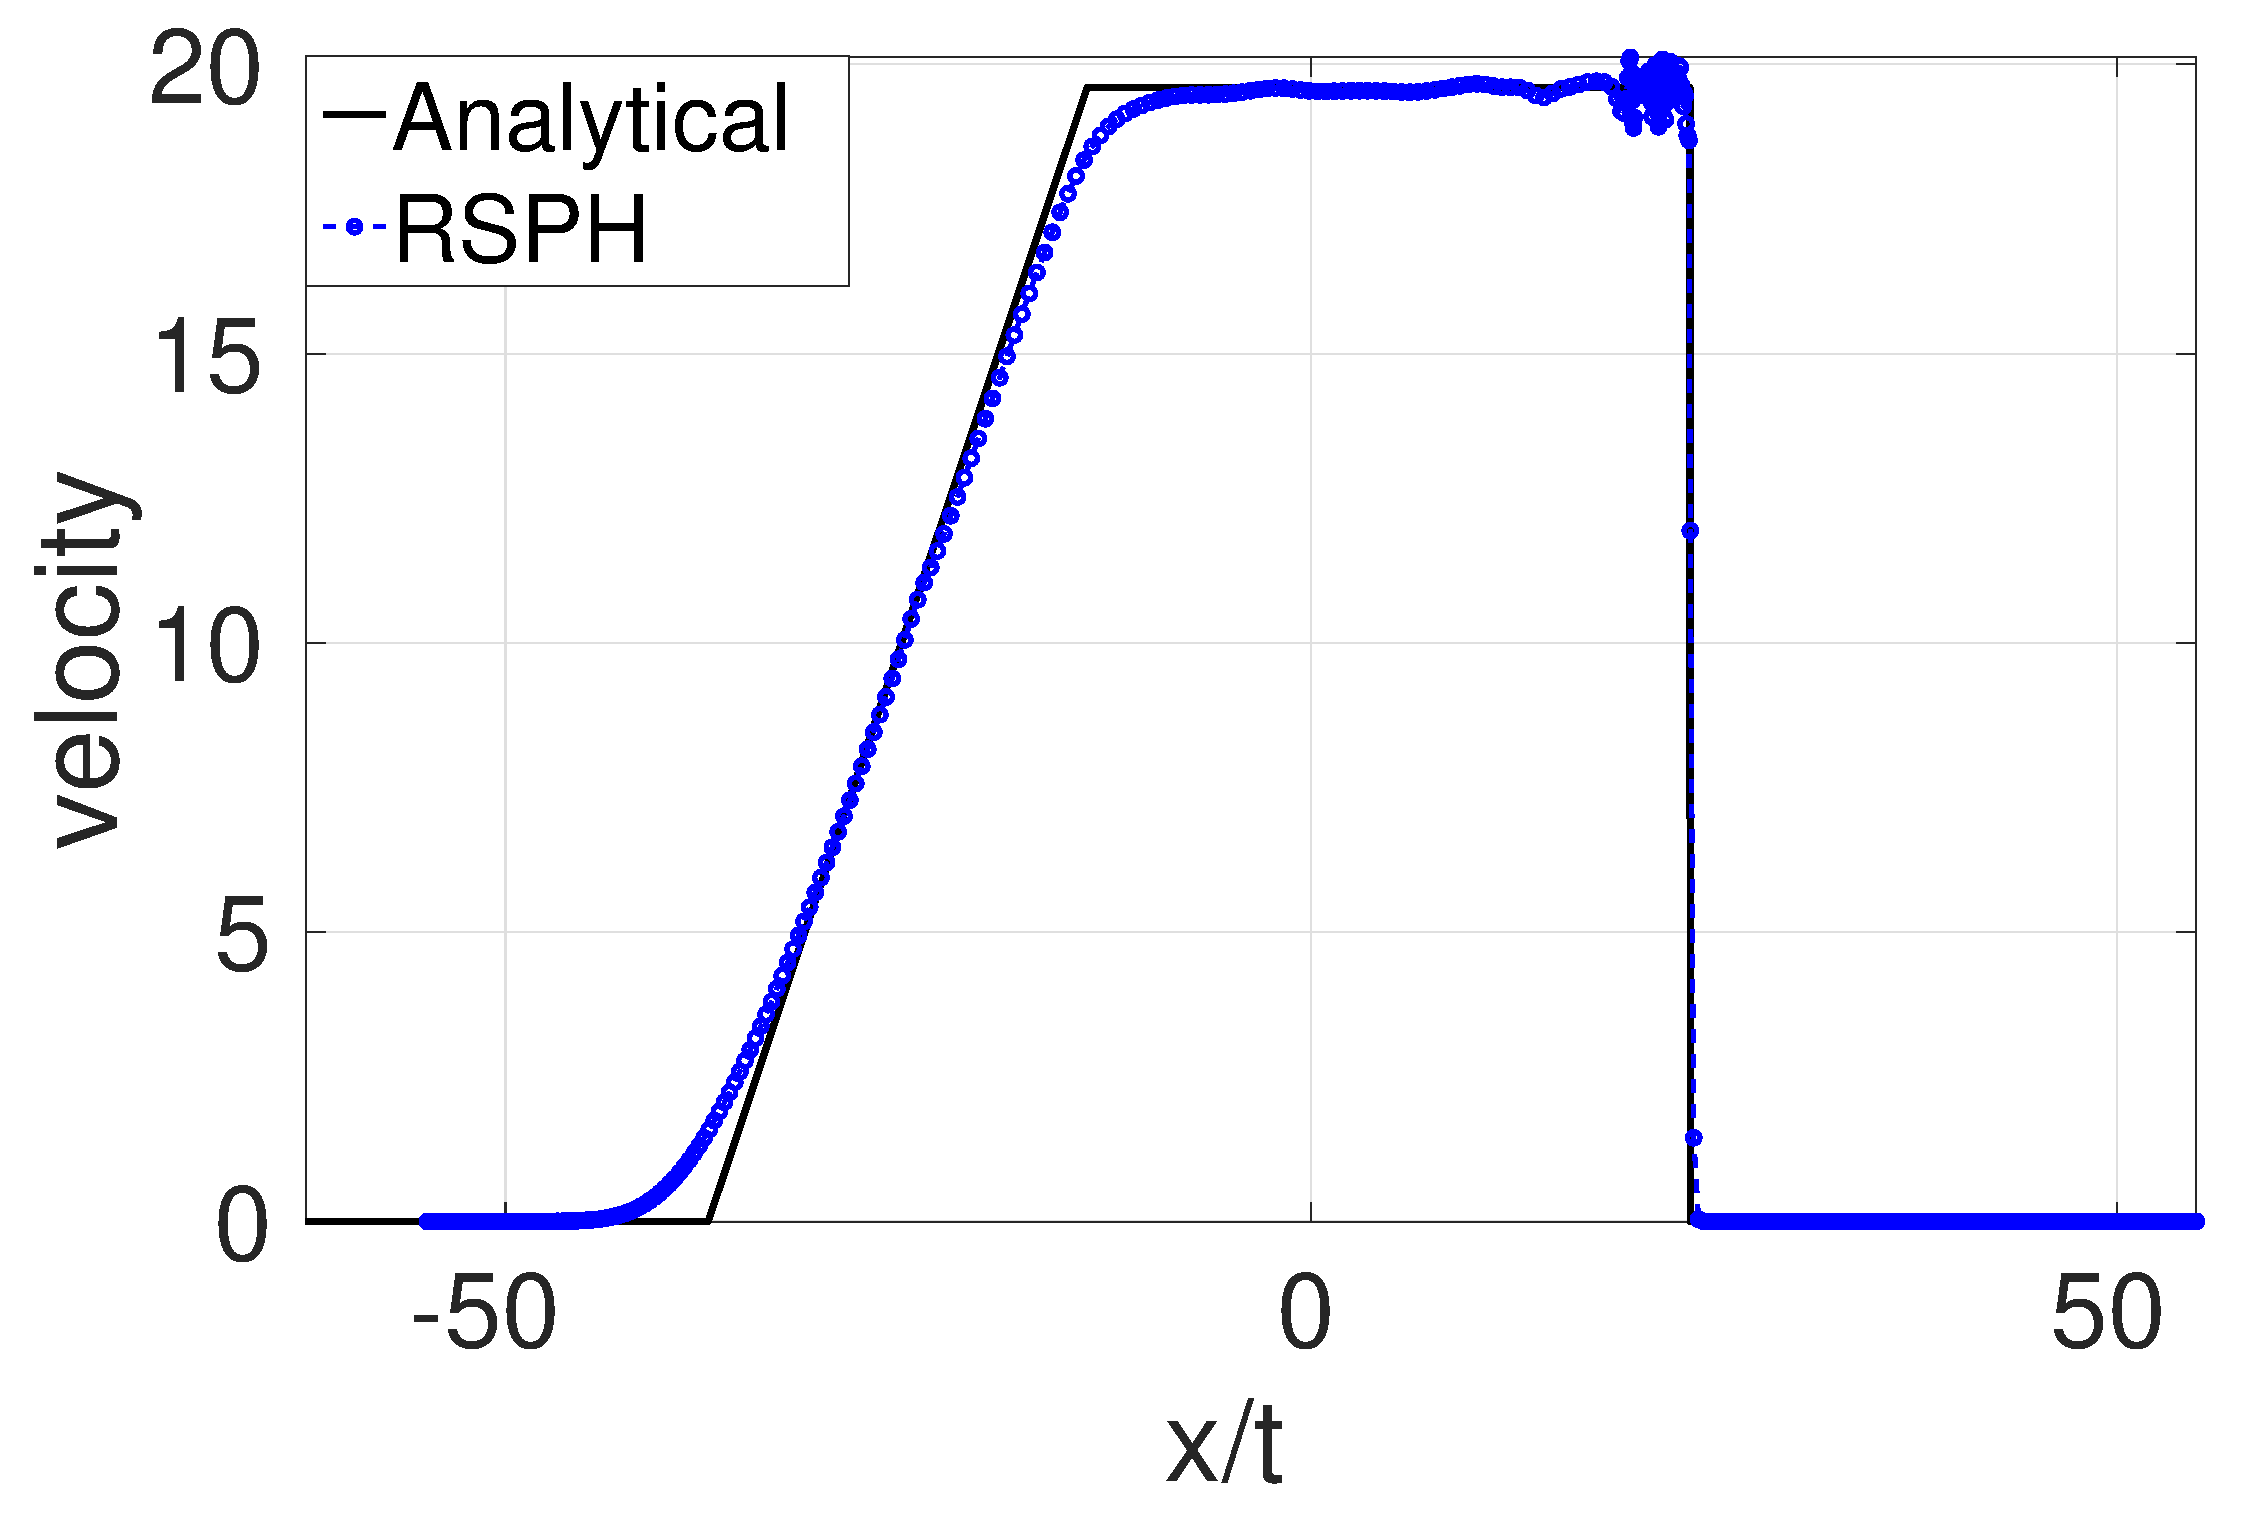
\includegraphics[width=0.99 \textwidth]{./Chapter-4/Figures/strong-blast/StrBlst-RCM-v-Rp3}
    \end{minipage}%
    \\
    \begin{minipage}{.415 \textwidth}
        \centering
        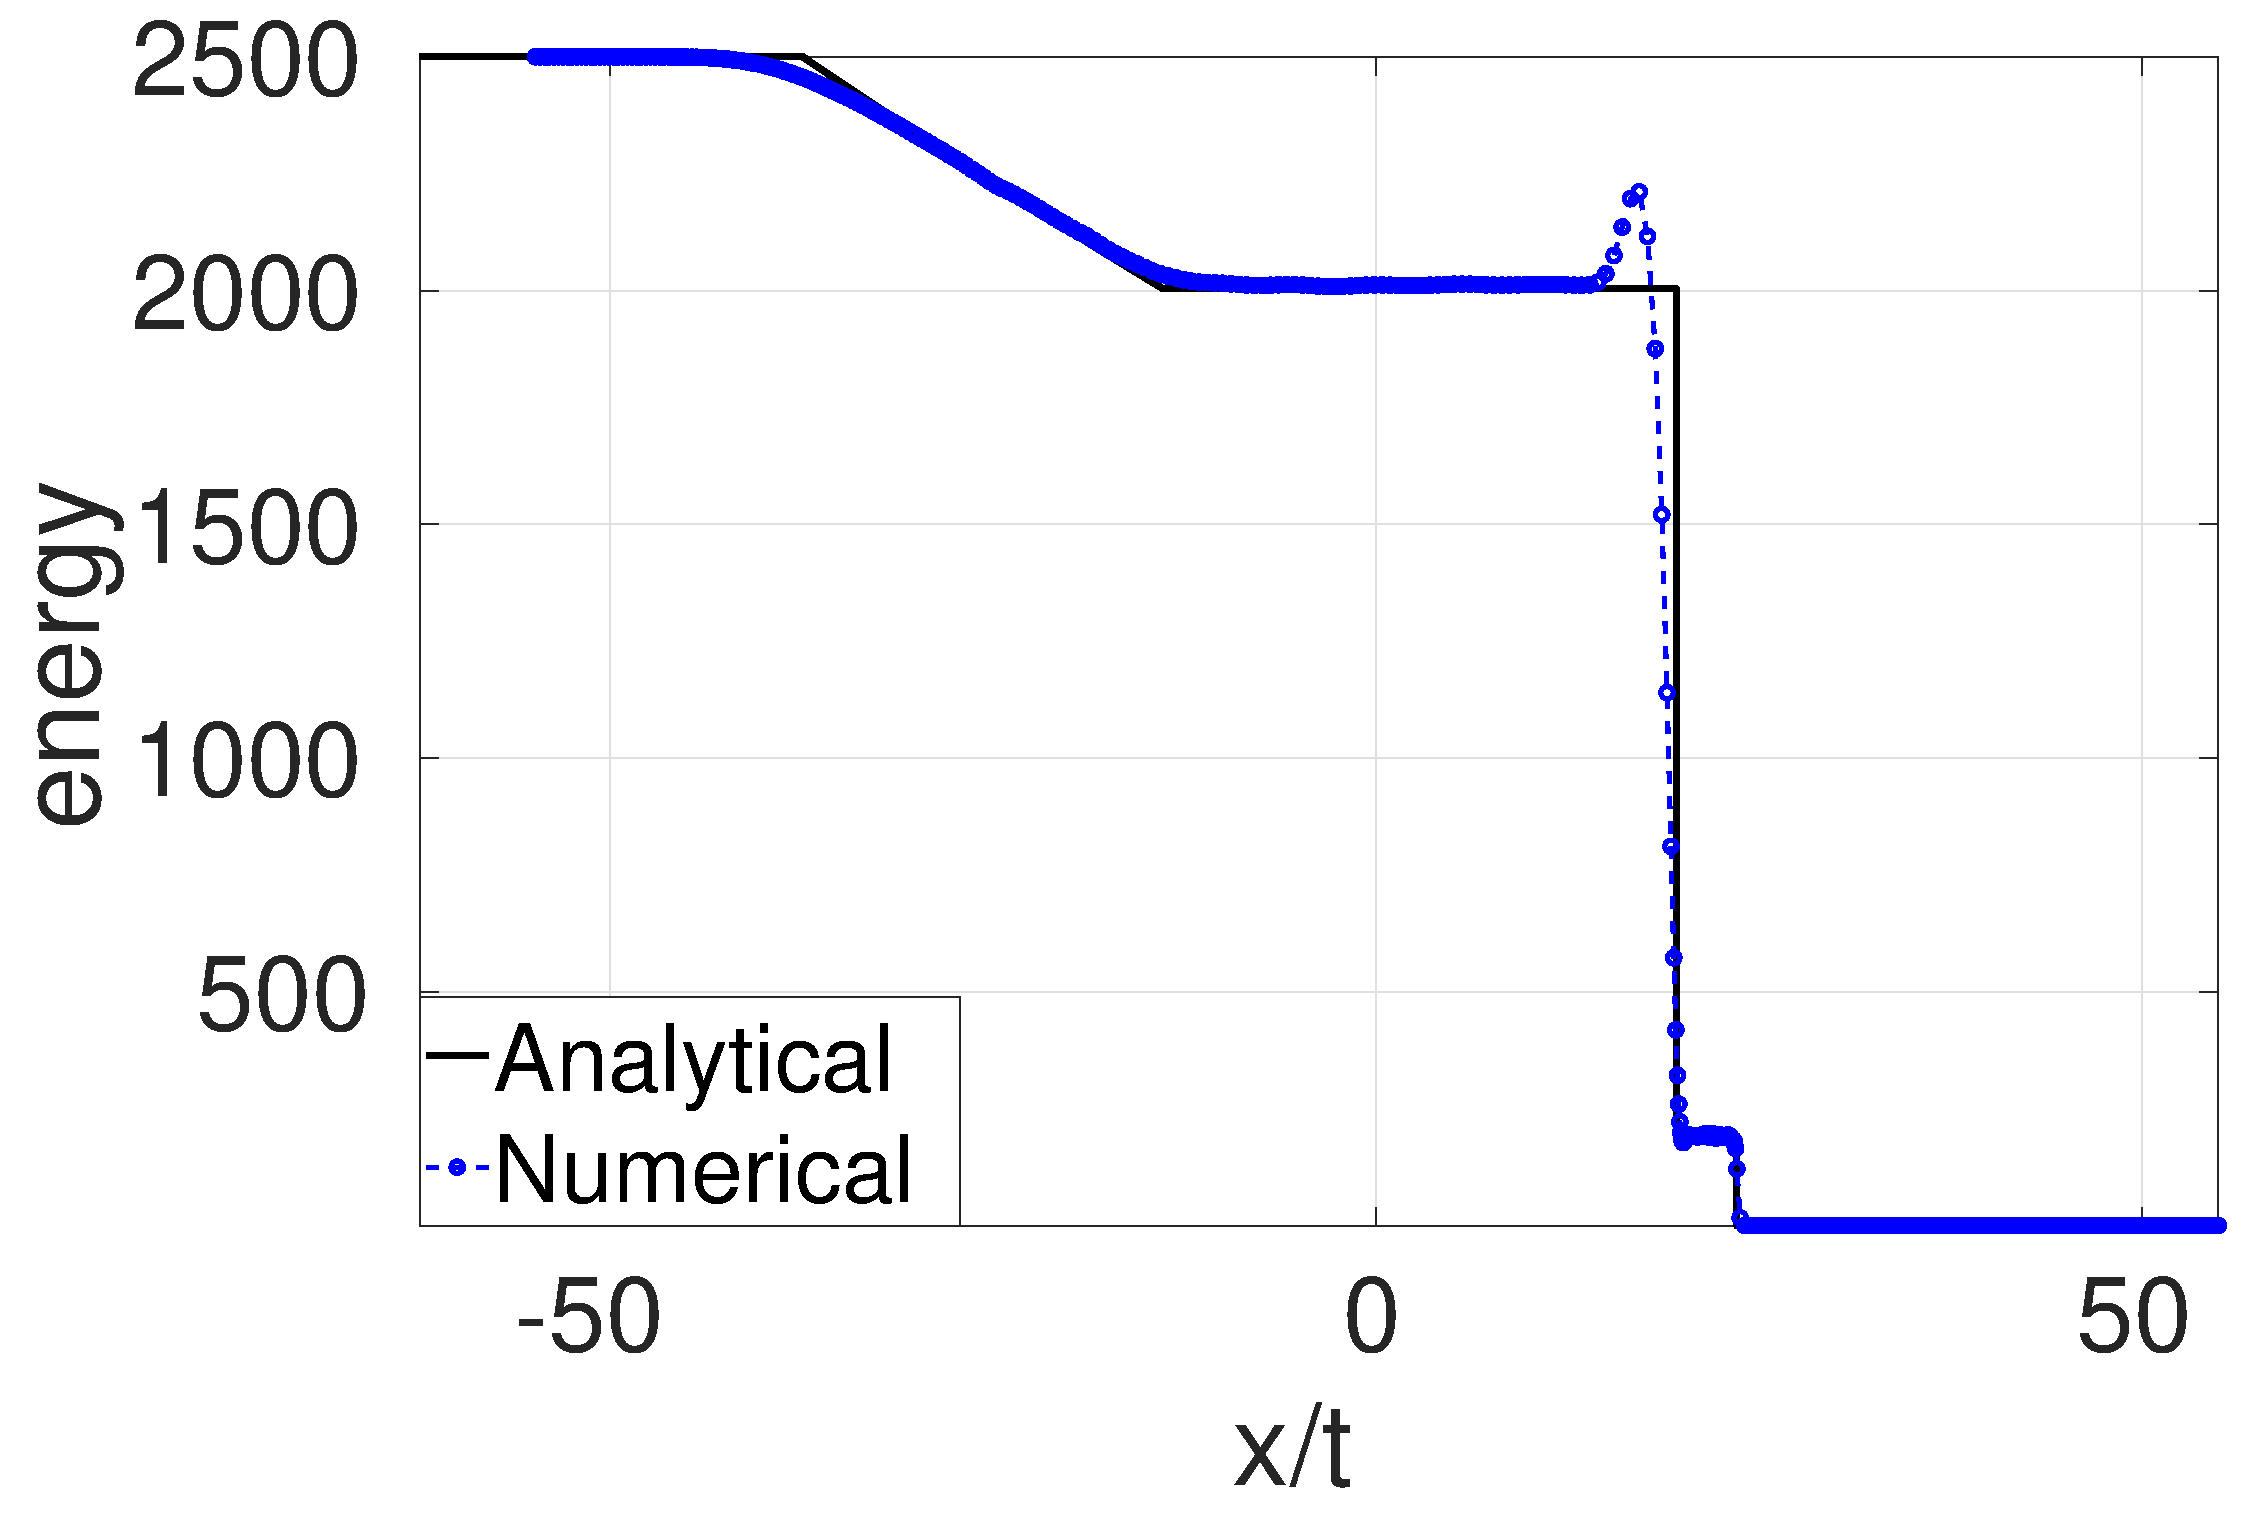
\includegraphics[width=0.99 \textwidth]{./Chapter-4/Figures/strong-blast/StrBlst-RCM-e-Rp3}
    \end{minipage}%
    \begin{minipage}{.415 \textwidth}
        \centering
        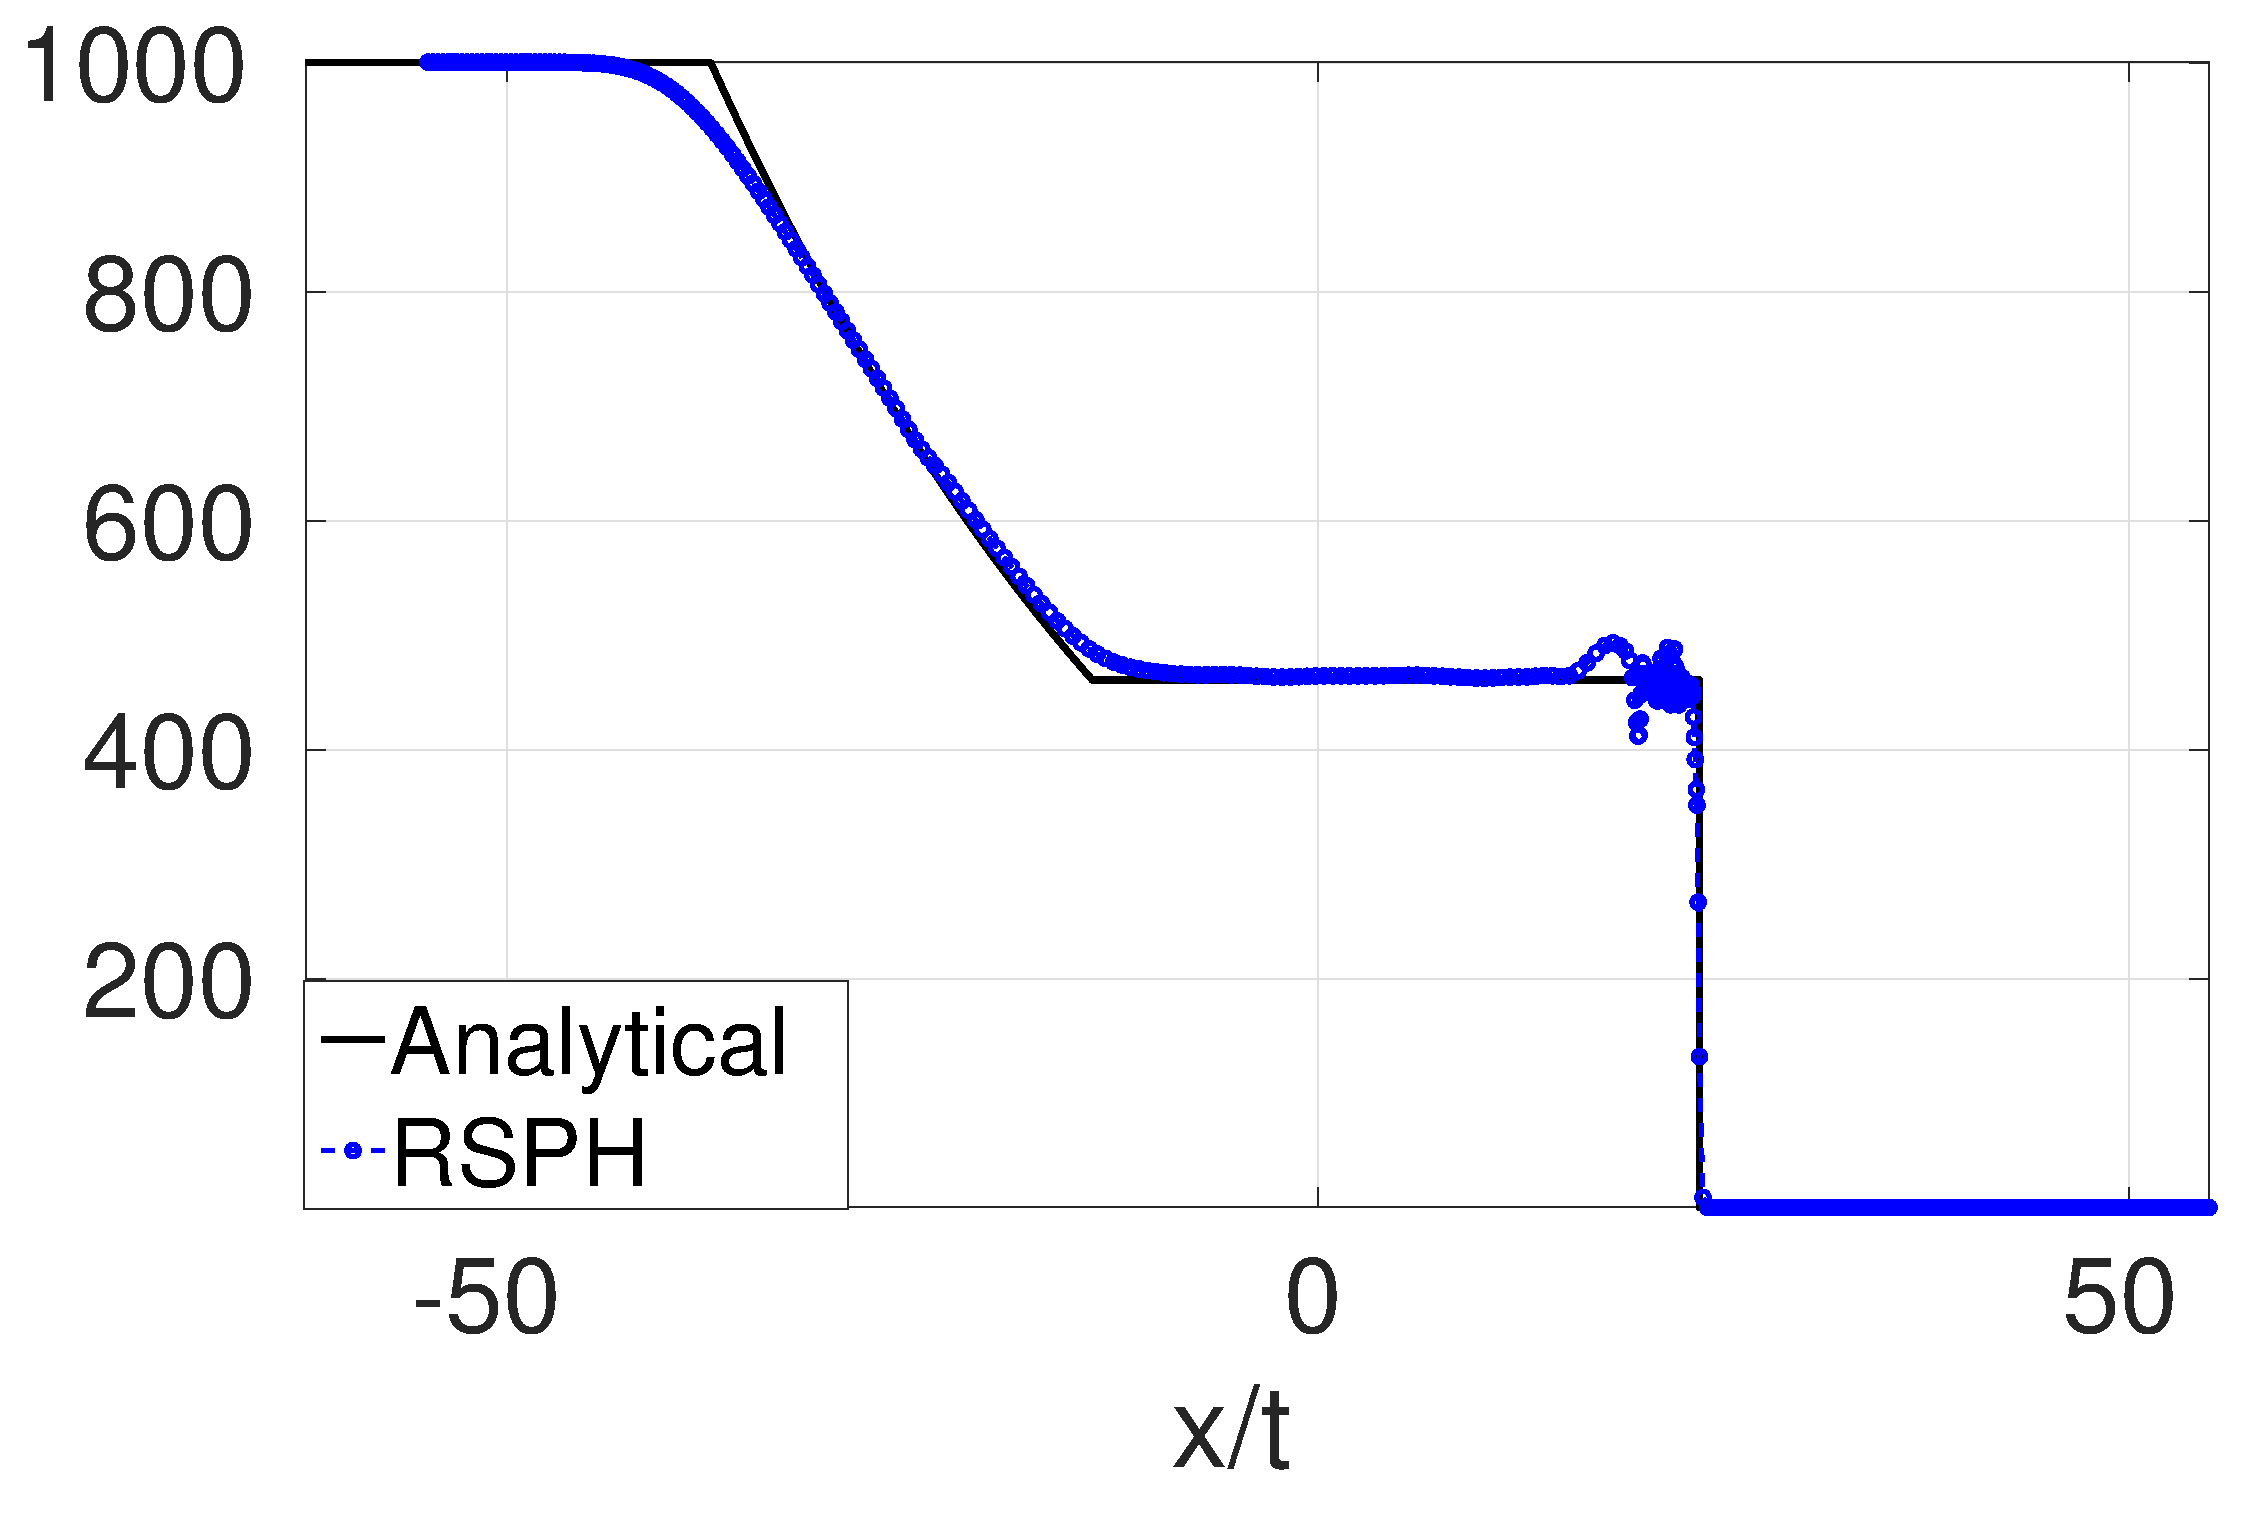
\includegraphics[width=0.99 \textwidth]{./Chapter-4/Figures/strong-blast/StrBlst-RCM-p-Rp3}
    \end{minipage}% 
    \caption{Results for test 6, the strong blast test. y axis for density plot is in log base 10.  To stabilize the simulation, RSPH sampling is in a narrower range. All physical properties are well re-produced. The oscillations between shock and contact discontinuity is relatively larger than other area. A noticeable spike is observed near contact discontinuity.}
    \label{fig:RCM-strong-blast}
\end{figure}

\subsection{3D free jet} \label{jet}
Free jet flow have been studied analytically, experimentally and numerically for many decades, not only because of its wide application but also because of its fundamental significance as a basic flow to the scientific research community. To test the capacity of RSPH for multiple dimensional applications, a free jet flow is simulated in this section by solving 3D compressible Euler Equations using standard SPH, GSPH and RSPH. We have to mention that the 3D free jet retains several features of volcanic plume development, such as mixing between erupted fluids and ambient fluids.
All simulations are using the same setting-up and compared at the same physical time. In this test, RSPH simulation is carried out based on piece wise constant construction of Riemann problem and a HLLC approximate Riemann solver. To do a well-controlled comparison, GSPH adopts the same way for Riemann problem construction and the same Riemann solver as RSPH. 

Similar to volcanic plume model described in Section \ref{sec:chp2-Mathematical-Description}, the computational domain in this test is a box. The boundaries can be categorized into the velocity inlet (a circular area at the center of the bottom of the box), no-slip wall boundary (box bottom) and pressure outlet (other faces of the box).
At the vent, exit velocity $\textbf{v}$ is set to $500 m / s$ and radius of the nozzle $r$ is set to $8m $. The pressure of ejected fluid is assumed to be the same as ambient ($101 kpa$). The temperature of ejected fluids and ambient fluids are set to $273 K$. 
Boundary conditions are imposed in a similar way as described in Section \ref{sec:SPH-bc}

\begin{figure}
    \centering
    \begin{minipage}[t]{.325\textwidth}
        \centering
        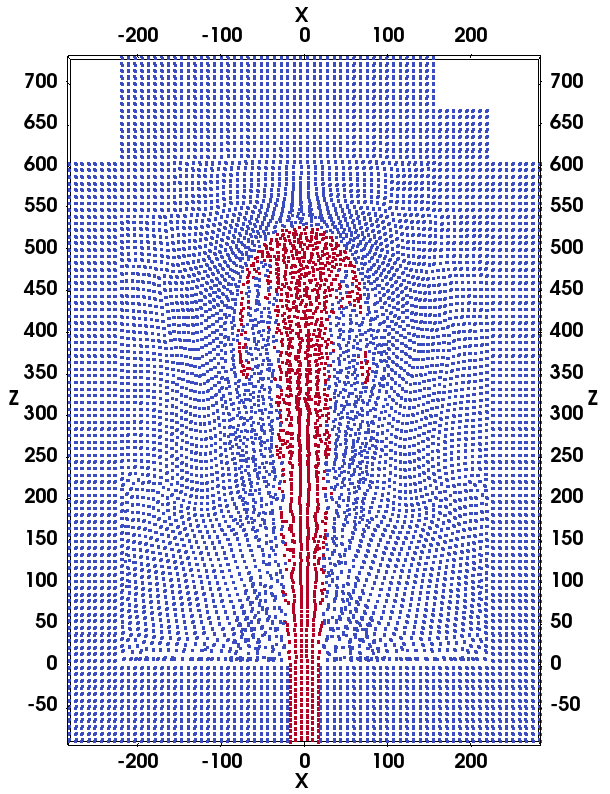
\includegraphics[width=0.99 \textwidth]{./Chapter-4/Figures/SPH-alf2-t3-cutView}
    \end{minipage}%
    \begin{minipage}[t]{.325 \textwidth}
        \centering
        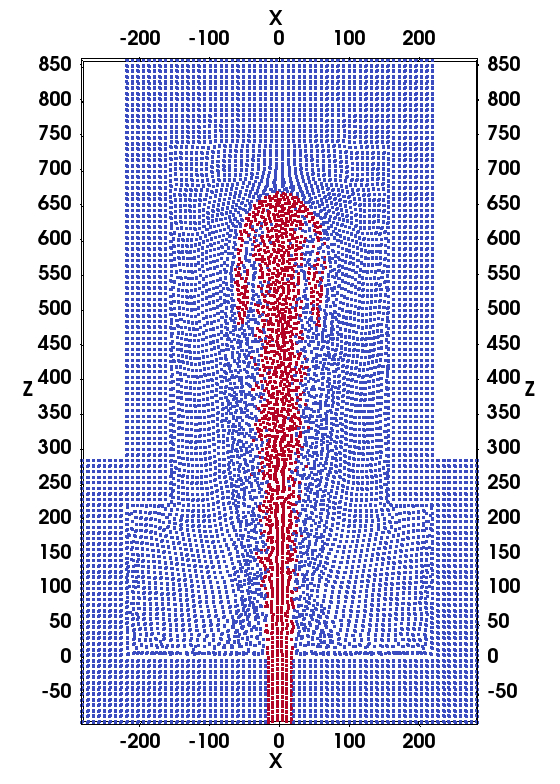
\includegraphics[width=0.99 \textwidth]{./Chapter-4/Figures/SPH-alf1-t3-cutView}
    \end{minipage}%
    \begin{minipage}[t]{.325\textwidth}
        \centering
        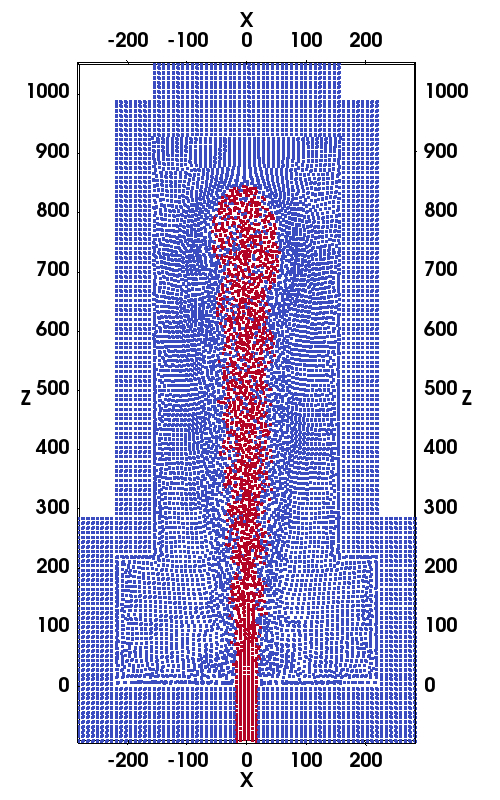
\includegraphics[width=0.99 \textwidth]{./Chapter-4/Figures/SPH-alfp3-t3-cutView}
    \end{minipage}%
    \caption{Free jet flow simulation results at $t=3.0 s$ by SPH using different artificial viscosity coefficients. These pictures are front view of a slice of the domain cut by two planes parallel to $x-z$ plane at $y=-9$ and $y=9$. From left to right, the picture is corresponding to $\alpha=0.3$, $\alpha=1.0$ and $\alpha=2.0$ respectively. Another artificial viscosity coefficient $\beta$ is set to be double of $\alpha$ for all tests. Red particles in pictures are particles erupted from the nozzle while blues are ambient fluids particles.}
    \label{fig:free-jet-SPH-comparison}
\end{figure}

\begin{figure}
    \centering
%    \begin{minipage}[t]{.325\textwidth}
%        \centering
%        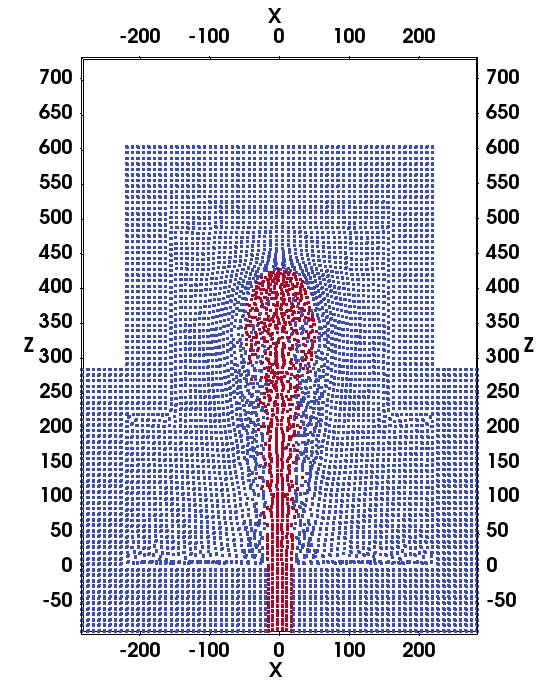
\includegraphics[width=0.99 \textwidth]{./Chapter-4/Figures/SPH-alf1-t1p5-cutView}
%    \end{minipage}%
    \begin{minipage}[t]{.325 \textwidth}
        \centering
        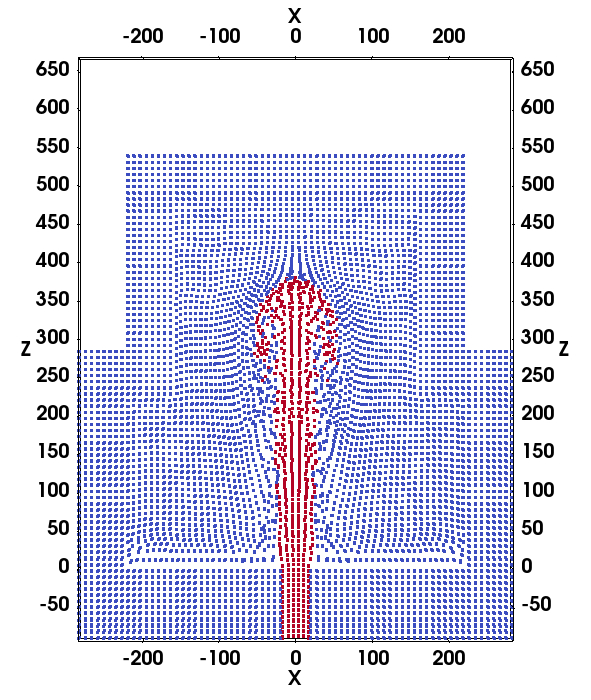
\includegraphics[width=0.99 \textwidth]{./Chapter-4/Figures/GSPH-HLLC-t1p5-cutView}
    \end{minipage}%
    \begin{minipage}[t]{.325\textwidth}
        \centering
        \includegraphics[width=0.99 \textwidth]{./Chapter-4/Figures/RSPH-t1p5-cutView}
    \end{minipage}%
    \\
    \centering
%    \begin{minipage}[t]{.325\textwidth}
%        \centering
%        \includegraphics[width=0.99 \textwidth]{./Chapter-4/Figures/SPH-alf1-t3-cutView}
%    \end{minipage}%
    \begin{minipage}[t]{.325 \textwidth}
        \centering
        \includegraphics[width=0.99 \textwidth]{./Chapter-4/Figures/GSPH-HLLC-t3-cutView}
    \end{minipage}%
    \begin{minipage}[t]{.325\textwidth}
        \centering
        \includegraphics[width=0.99 \textwidth]{./Chapter-4/Figures/RSPH-t3-cutView}
    \end{minipage}%
    \caption{Simulation results of free jet flow by GSPH and RSPH. These pictures are front view of a slice of the domain cut by two planes parallel to $x-z$ plane at $y=-9$ and $y=9$. From left to right, the picture is corresponding to SPH, GSPH and RSPH respectively. Red particles in pictures are particles erupted from the nozzle while blues are ambient fluids particles. Pictures on the first row are corresponding to $t=1.5s$ while pictures on the second row are for $t=3.0 s$}
    \label{fig:free-jet-comparison}
\end{figure}

Figure \ref{fig:free-jet-SPH-comparison} shows simulation results of the free jet flow by SPH with different artificial viscosity coefficients. The overall damping effect due to artificial dissipation is clearly shown in this figure. We observe that the lengths to which these jets reach at $t=3.0 s$ are different when using different artificial viscosity coefficient. It is obvious that the larger artificial viscosity, the shorter length the jet can reach. The length that free jet reaches can be used as an indicator of overall dissipation. While introducing undesirable damping effects, artificial viscosity is necessary for numerical stability and simulating of shocks. So, in real applications, the artificial viscosity coefficients are usually tuned (see, for example, \citep{gmd-2017-119}) to minimize artificial damping effects.

We compare RSPH with GSPH in terms of equivalent overall artificial damping effects in Fig. \ref{fig:free-jet-comparison}. Different from SPH, both GSPH and RSPH introduce artificial viscosity in an implicit way by solving local Riemann problems. As has been shown in 1D tests, RSPH can introduce less artificial viscosity than GSPH. Fig. \ref{fig:free-jet-comparison} implies that RSPH introduces less overall damping effect than GSPH in 3D application as well, which is consistent with 1D tests. That is to say, RSPH's desirable property of introducing less artificial dissipation in 1D unsteady flow is inherited in 3D applications of RSPH. Recall that RCM shows ability of resolving discontinuities as true discontinuities in 1D unsteady flows but such very desirable property does not persist in genuine two (or higher) space dimensions \citep{colella1982glimm}. Integrating of RCM within the framework of SPH avoids solving higher dimensional Riemann problems overcoming the fundamental shortcoming of RCM.

\section{Conclusion} \label{discussion}
In this chapter we have proposed RSPH, a novel SPH scheme for solving hyperbolic non-linear PDEs that combines the Random Choice Method with an approximate Riemann solver. No explicit artificial viscosity is needed. Instead, any viscosity that is used in a hydrodynamics simulation is just what the user implicitly adds. 
This control is important in applications with very strong shocks. 
Unlike classical SPH which uses the same artificial viscosity coefficients everywhere, RSPH introduces larger dissipation around the shock to guarantee numerical stability while introduces much smaller dissipation elsewhere. Such adaptive manner of assigning dissipation reduces unnecessary numerical damping but preserves demanded damping for restraining numerical instability. As demonstrated in 1D and 3D tests, RSPH causes less smearing of shocks and less overall dissipation for jet flow.
In addition, RSPH also shows good convergence behavior.

On the other hand, RSPH does not address other methodological questions that must be decided in order to use SPH, questions such as the smoothing length of the SPH kernel. We have investigated the HLLC approximate Riemann solver in this chapter; it is of interest to test other approximate solvers, to better understand the behavior of solutions. This may be particularly important when applying RSPH to other systems, where the explicit construction on which the HLLC solver rests is not readily available.
\chapter{Code Architecture and Parallelism} \label{chapter:architecture-parallelism}

\section{Introduction}
\label{sect:introduction}
Accurate prediction of volcano plume development in a given time window requires resolution (very high particle counts) that can not be accomplished without parallel computing. Imposing some types of boundary conditions (such as wind field, eruption boundary condition at the vent) requires dynamically adding and removing particles during simulation. This requires an efficient and flexible data management scheme. This chapter will present the architecture that enables efficient and flexible data management and algorithms for solver parallelization.

Most implementations of the parallel SPH method presented to date are limited to standard SPH and benchmark problems like dam breaks, or relatively simple scenarios like breaking-waves, flooding, etc. Work on more complicated implementations is relatively rare. The demands of flexible data access are scarcely addressed. Among existing CPU parallel SPH schemes, most of them focus on neighbor searching algorithms and dynamic load balancing. (eg. \citep{ferrari2009new, crespo2015dualsphysics}). Less attention has been paid to developing more flexible data management schemes. 
Fortunately, efficient and flexible data management strategies for parallel computing have been successfully implemented in mesh based methods (eg. \citep{laszloffy2000simple} for adaptive hp finite element method (FEM), and \citep{patra2005parallel} for finite volume method (FVM)). Motivated by these techniques developed for mesh based methods, we present a complete framework for parallelizing SPH program with the MPI standard allowing flexible and efficient data access.\\
Any implementation of SPH requires efficient searching and updating of neighbors during the simulation. Of the many possible choices we adopt the popular background grid method \citep{monaghan1985refined}, which is also used for domain decomposition. We refer to the elements of the background grid as buckets. 
As for the actual storage of data representing the physical quantities associated to each particle, different strategies have been adopted in existing implementations of SPH. 
In DualSPHysics \citep{crespo2015dualsphysics}, the physical quantities of each particle (position, velocity, density...) are stored in arrays, and the particles (and the arrays with particle data) are reordered following the order of the cells. It is not flexible enough to add, delete and especially access particles for such fixed-size arrays. \citet{ferrari2009new} adopted linked lists using pointers so that particles can be deleted or added during the simulation. Storage problems caused by fixed-size arrays are thereby also eliminated. We adopt hash tables to store pointers to objects of particles and buckets, which give us not only flexibility of deleting and adding of elements, but also quicker access compared with linked lists. A SFC-based index is adopted to give each particle and background bucket an unique identifier -- a strategy known to preserve some locality at minimal cost. The SFC based numbering strategy is further extended to include time step information so that particles added at the same position but different time will have different identifiers. 
We adopt an easy-programming scheme based on SFC \citep{patra1999efficient} to decompose the domain.

To the best of the author's knowledge, no current implementation of SPH has the feature of adjusting the computational domain based on simulation needs. For volcano plume simulation, this feature will greatly reduce computational cost by avoiding computing of uninfluenced fluids. This feature is accomplished by adding a scan function to monitor the outermost layer of the domain and turn ghost particles to real particles at the proper time thus effectively defining a halo domain with an almost optimally defined size.

\section{Workflow}
\begin{figure*}[!t]
\centering
\includegraphics[scale=0.43]{Chapter-5/Figures/Work_flow}
\hfil
\includegraphics[scale=0.43]{Chapter-5/Figures/Work_flow_adjust}
\caption{Workflow for SPH code. Figure to the left is the basic workflow. The right figure is the workflow that enables dynamic halo domain. These steps in orange box are newly added steps. Extra computational costs associated with these extra steps are discussed in section \ref{sec:effect-of-halo-domain}}
\label{fig:Work_flow}
\end{figure*}

In SPH, the domain is discretized by particles and the position of each particle is updated at every time step. The governing equations are estimated as sums over particles in a compact subdomain defined by the support of the kernel function. Only particles located within the support of the kernel function will interact. Thus, physical properties associated with the particle are updated based on its neighbors. A neighbor search therefore needs to be carried out before updating physical properties. Figure \ref{fig:Work_flow} shows the basic workflow of our SPH code, which includes three sections in the major updating loop: pre-updating section (neighbour searching and updating wall boundary conditions), physical quantities updating section and domain repartition section. Adding of new eruption ghost particles is carried out right after particle position updating in the updating section. Pressure outlet boundary condition is setup at initial condition setup step and dose need to update during simulation.
We use buckets, which contain all particles associated with a sub-domain (see Fig. \ref{fig:SFC_domain_decomposition}) 
and keep them stationary during the entire simulation, to reduce neighbour searching cost (since the search can now be restricted to only neighboring domains). No physical quantities are associated with bucket.

Domain is also partitioned based on the background mesh, whose elements are buckets containing the discretization points. Domain is decomposed by cutting SFC going through centroids of all buckets, as shown in Fig. \ref{fig:SFC_domain_decomposition}.
Data synchronization is carried out after every updating. Computational load of each subdomain is evaluated by summing up calibrated particle weights. Computational domain is re-decomposed to restore load balance when necessary.
In current implementation, domain repartition is not carried after every time, instead, at an optimized interval.

The basic elements, particles and buckets, are identified by unique ID that generated based on SFC. All data are managed by hash tables, with external linked list to handle hash conflict. SFC is also used to decompose the computational domain.


\section{Data management and parallelization}
\subsection{SFC based indexing}
Our data structure starts from assigning each particle and bucket an identifier, we refer to it as a key, which should be unique throughout the simulation. The key for a bucket is determined by the centroid coordinate of the bucket while the key for a particle is determined by adding coordinates and time step of the particle. The map from coordinates to key is based on SFC \citep{sagan2012space} which maps a n-dimensional domain to a one dimensional sequence. The standard procedure for obtaining the SFC is: 
\begin{itemize}
\item Scale all coordinates in computational domain ($\textbf{X}^\prime$) into an $n$ dimensional unit hypercube $[0,1]^n $: $\textbf{X}^\prime \rightarrow \textbf{X}$, where $\textbf{X}$ represents coordinates in the hypercube.
\item Compute $k_r = h_n(\textbf{X})$. Where $h_n$ is the map $h_n: [0,1]^n \rightarrow [0,1]$. 
\item Convert $k_r$ to integer $k$ by multiplying $k_r$ with a large integer and removing decimal part.
\item Sort all keys to form a SFC sequence. The SFC represents a curve passing through all particles (or centroids of buckets).
\end{itemize}
%
\begin{figure*}[!t]
\centering
\includegraphics[scale=0.26]{Chapter-5/Figures/SFC_particles_buckets}
\hfil
\includegraphics[scale = 0.275]{Chapter-5/Figures/SFC_particles_buckets_partition}
\caption{The left figure shows SFCs passing all particles and buckets. The right figure shows an example of a domain decomposition based on the SFC of buckets.}
\label{fig:SFC_domain_decomposition}
\end{figure*}

Details for constructing the map $h_n$ can be found in \citep{patra1995problem}. These keys denote a simple addressing and ordering scheme for the data, i.e., a global index space for all the objects.

In some situations, new particles need to be added during the simulation. For example, new particles need to be added at the bottom of the eject vent (see Fig. \ref{fig:Particle_adding_with_link}). To assign distinct identifiers for particles added at the "same position" but at different time steps, we extend the SFC-based key to a time-dependent SFC based key by including date of birth of particles into their keys. The time-dependent SFC based key can be denoted as: $[k,t]$, where $t$ is the time step. The map $h_n$ will become:
\begin{equation}
h_n: [0,1]^n \times \textbf{T} \rightarrow [0,1] \times \textbf{N}
\end{equation}
Where $\textbf{T} \subset [0,\infty)$ is the time dimension, and $\textbf{N}=\lbrace 0, 1, 2, 3...\rbrace$.
To guarantee locality, sorting of particle keys is based on $k$, that is to say, particles with smaller $k$ always come before particles with larger $k$. For particles that have the same $k$, ordering will then depend on $t$. Figure \ref{fig:SFC_domain_decomposition} shows SFC ordering of buckets and particles in buckets. 
Several features of this indexing scheme are suitable for SPH:
\begin{itemize}
\item Guaranteed uniqueness of keys.
\item The key of each object is generated purely based on its own coordinates. When we add new objects on different processes, the key of each object can be generated fast and independently.
\item Objects that are located closely in the Euclidian space will also be close to each other in the one dimensional SFC key space in a mean sense. Since SPH particles only interact with their neighbors, geometric locality can be exploited for efficient access of data.
\item This type of key effectively generates a global address space. Globalism of key and conservation of spatial locality make it easy to partition the sorted key sequence and obtain a decomposition of the problem.
\end{itemize}

The (time-dependent) SFC based indexing plays central pivot role in the architecture. Besides creating unique ID efficiently and independently, SFC based domain decomposition helps preserve spatial locality making it very easy to design a hash function that preserve such locality in memory. The globalism of such indexing, which is also inherited in hash table, greatly simplifies complexity when moving elements around. As index generating (hence hashing) is independent and fast, creating/deleting of element are efficient and flexible.
All these features help keep the overall architecture brief, robust and sustainable.

\subsection{Data management strategies}
\subsubsection{Particle and bucket}
The most basic data structure of SPH are particles and buckets. Both are defined as C++ classes. Information that is contained in particle objects can be categorized into six categories: identifier (the key), affiliate(rank of the process that the particle belongs to), primitive variables (variables in governing equations, e.g. density, velocity), secondary variables (physical properties that can be computed from primitive variables, they are stored to avoid repeated computations, e.g., pressure and temperature), flags (indicators, such as indicator for ghost particle or real particle) and neighbor information (it is a vector of particle keys in our application). Similarly, information that is contained in a bucket object can also be categorized into different categories: identifier, affiliate, dimension information (maximum and minimum coordinates, boundary information), flags (indicators, such as guest indicator, which is used to indicate whether the bucket belongs to another adjacent subdomain or not), neighbor information (keys of 27 neighbor buckets including its own key) and owned particles (it is a vector of particle keys in our application).
Using of several independent flags creates a multiple-dimensional categorization space which enables flexible elements categorization simplifing algorithms.
Objects of particles and buckets are then accessed through hash tables.

\subsubsection{Hash table and hash collision}
Several data structures have been considered for actual data storage. Vector and array can guarantee efficicent and flexible element access while inserting of new elements is either expensive or not allowed. List type of data structure allows flexible and efficient new element insert but element access is expensive ($(O(n)$).
Hash table guarantees fast element access ($(O(1)$) while allows flexible and efficient new element insert. Hashmap also allows flexible and efficient new element insert, but its element access is a little more expensive($(O(logn)$). We finally choose to use hash table, which is essentially a chunk of memory with many slots. The pointer to certain element object is stored in one slot. Based on the keys of data, the address-calculator(hashing) function determines in which slot the data should be stored:
\begin{equation}
Index = hash(key)
\end{equation}

Data in a hash table can be accessed with time complexity of $O(1)$ when there is no hash collision. One way to handle hash collisions is to use an additional sorted vector attached to the hash table. When several keys hash to the same index, a vector will be created. The vector is sorted based on keys so that a binary search (with an average time complexity of $O(log n)$) can be used to find the correct position for adding, deleting or retrieving of data. Another option is using an additional linked list which is more flexible in memory allocation but slower in searching $(O(n)$). In addition, pointer based memory accessing of linked lists will greatly slow down the efficiency of data access for long linked lists. Choosing the proper way to handle hash conflicts greatly depends on the problem itself. For volcano plume simulation, new particles are added at the bottom of the eruption vent (see Fig. \ref{fig:Particle_adding_with_link}), making the linked list a better choice. Pointers to these new particles will be stored in external linked lists as shown in Fig. \ref{fig:Particle_adding_with_link}.
\begin{figure}
\centering
{\includegraphics[scale=0.42]{Chapter-5/Figures/Particle_adding_with_link}}
{\caption{Non-uniform distribution of particles in the $[0,1]^n \times \textbf{T}$ space due to adding of new particles at a small area of the whole domain.}
\label{fig:Particle_adding_with_link}}
\end{figure}

\begin{figure}
\centering
{\includegraphics[scale=0.45]{Chapter-5/Figures/int_bar}}
{\caption{The influence of different load balance check intervals on simulation time. The bar values are the extra simulation time in log scale. The optimized interval is 3s.}
\label{fig:check_int}}
\end{figure}

For time-independent keys, the hash function can be a simple function like:
\begin{equation}
Index= \frac{Key - Min\,Key}{Max\,Key - Min\,Key} 
\times Hash\,Table\,Size 
\label{eq:hash_function}
\end{equation}

One natural way to hash time-dependent keys $[k,t]$ is to convert the two elements in the key into one number taking $k$ as the higher digit and $t$ as the lower digit of the large number. However, for volcano plume simulation, only ghost particles for eruption boundary condition will be successively added at the same place: the bottom of the vent. That is to say, particles are distributed non-uniformly in the $[0,1]^n \times \textbf{T}$ space as shown in Fig. \ref{fig:Particle_adding_with_link}. To avoid a non-uniform sparse hash table and conserve spatial locality, we only plug the first number, $k$, of the key, $[k,t]$, into the hashing function, Eq. (\ref{eq:hash_function}). All particles with the same birth location will hash to the same slot and be handled by external linked lists.

\subsection{Domain decomposition and load balancing strategy}
\label{sect:load_balance}
\subsubsection{Weighted work load} \label{sec:Weighted_work_load}
Particles in our problem can be categorized into four types: real particles, wall ghost particles, pressure ghost particles and eruption ghost particles. Ghost particles are for imposition of corresponding boundary conditions (See Fig. \ref{fig:Plume}). As different types of particles involve different amount of computational work, shown by table \ref{tab:Computational_cost_steps}, we assign different work load weights for different types of particles based on profiling data. Instead of simply using number of contained particles as work load for buckets, work load of each bucket is determined by summing up work load weights of all particles within the bucket.
\begin{equation}
W^{bucket} = \sum_i^{N^{particle}} W_i^{particle}
\label{eq:work-load-bucket}
\end{equation}
where $N^{particle}$ is total number of particles contained by the bucket. $W_i^{particle}$ is weight of particle, depending on particle type (see Table \ref{tab:Computational_cost_steps}).
The SFC of buckets now becomes a weighted sequence. Domain decomposition is conducted by cutting the weighted SFC of buckets into pieces.

\begin{figure}
\centering
%\CenterFloatBoxes
%\ttabbox
%{	  
	  \begin{tabular}{lrrrrrr}
	    \hline
	    Step & Cost ($ms$) & Real & wall & eruption & pressure\\
	    \hline
	    neighbor search & 0.41 & Yes & No & No & No \\
	    update momentum and energy & 0.70 & Yes & No & No & No\\
	    update density & 0.42 & Yes & No & No & No \\
	    update position & 0.01 & Yes & No & Yes &  No\\
	    velocity filtering& 0.43 & Yes & No & No & No\\
	    apply wall boundary condition     & 0.75 & No & Yes & No & No\\
	    summation ($ms$) & - & 1.97 & 0.75 & 0.01 & 0.00\\
	    \hline
	  \end{tabular}
%}
{\caption{Computational cost per particle for different steps}	}
\label{tab:Computational_cost_steps}
\end{figure}

\subsubsection{Domain decomposition and dynamic load balancing}
Figure \ref{fig:SFC_domain_decomposition} shows how the domain is decomposed based on partition of the SFC of buckets. The particles are automatically split into several groups along with buckets that contain them. As the SFC of buckets is a curve in 3D space, partition of this curve will automatically lead to 3D domain decomposition. Each piece of the SFC after partitioning, which will be calculated by each processor, should then have a balanced total work load. That is to say:
\begin{equation}
W^{process}_1 \approx W^{process}_2 ... \approx W^{process}_i ...\approx W^{process}_{N^{process}}
\label{eq:work-load-balance}
\end{equation}
where $N^{process}$ is total number of processors, work load of each processor is calculated according to Eq. (\ref{eq:work-load-process}).
\begin{equation}
W^{process} = \sum_i^{N^{bucket}} W_i^{bucket}
\label{eq:work-load-process}
\end{equation}
where the work load of each bucket is evaluated based on Eq.(\ref{eq:work-load-bucket}).

As some of the neighbor particles reside in other partitions, a set of ``guest'' particles and buckets are used to synchronize data across partitions. To minimize communications, data is synchronized only after updating of physical quantities and positions or after repartition. Data associated with a single particle (or bucket) are first packed up before send out and then unpacked after receiving. In addition, not all information contained by element (bucket or particles) is packed. For example, secondary variables and neighbour information of particles are not send out. In this way, the amount of data that need communicate is reduced. Packed data will be loaded onto a bus (an array whose elements are packed buckets or particles) and send out once. Non-blocking MPI communications is adopted to reduce communication overhead.

Movement of particles, adding of new particles, and adjustments of domain will lead to significant load imbalance between processes. To restore load balance, computational load is monitored at a given interval which is optimized based on numerical experiments (see details in section \ref{sec:numerical-tests-computation}). Repartitioning is carried out when load imbalance is larger than a given tolerance.

\section{Dynamic halo domain} 
For plume simulation and similar phenomena, where some fluid ejects into a stationary fluid and gets mixed, the stationary fluid must be represented.
A lot of CPU time will be spent on computing associated with these stationary particles. If simulation of stationary particles can be avoided, the computational cost will be greatly reduced.
We propose a simple strategy to add such a feature to our code with low computational cost. We add a scan function to monitor the outermost layer of the domain. When the ejected fluid reaches the boundary of the current domain, pressure ghost particles (light blue particles in the right figure of Fig. \ref{fig:Plume}) will be turned to real particles (red particles in the right figure of Fig. \ref{fig:Plume}) and then add a new layer of pressure ghost particles for pressure boundary conditions. Wall ghost particles (grey particles in the right figure of Fig. \ref{fig:Plume}) will also be added when necessary. The original workflow is modified to enable such a feature. The modified workflow is shown on the right in Fig. \ref{fig:Work_flow}).

An involvement flag is added to particle class to distinguish different states of involvement. Particles are categorized into three groups based on the value of the involvement flag: involved, potentially involved, and not involved. The involved particles are particles that have already been affected by the mixing. The potentially involved particles are particles that have not been involved in mixing but are adjacent to involved particles and will thus be involved in the near future. 
All communication and computation associated with uninvolved particles can be ignored. That is to say, only potential involved and involved particles need to be simulated.
As simulation progresses, the ejected fluid will reach a larger area and more and more particles will be influenced. When originally stationary air is influenced by erupted material, the mass fraction of the erupted material will increase from zero to a positive value. So we can determine whether a particle should turn to involved status based on whether the mass fraction of that particle is larger than a given threshold ($10^{-5} $ in our simulation) or not. Based on such criteria, any real particles of phase 2 (erupted material) are qualified to be involved particles.  Particles of phase 1 (air) are also qualified to be involved particles if they are inside of the plume or close to the margin of plume. Other physical properties, like velocity, might also serve as alternative ``switch criteria''. Switching of particles from potentially involved to involed status is carried out right after mass fraction updating (the ``density update" step in left figure of Fig. \ref{fig:Work_flow}).

A similar scheme is also deployed for buckets resulting in a categorization of buckets. The additional complexity is that potentially involved ghost particles must also be taken into accounted. The switch criteria for bucket from potentially involved to involved is based on the fact whether the bucket contains any involved particles. Switching of bucket from potentially involved to involved is carried out in the a newly added step in the workflow, the ``Scan the Most Outside Layer
Buckets \& Return Adapt Indicator" step.

By implementing the algorithm of dynamics halo domain presented above, the computational domain grows dynamically during simulation. Figure \ref{fig:Plume} shows a cross-sectional view of a typical computational domain during simulation. As can be seen, the plume just fit into the computational domain, which has irregular geometry.

\begin{figure*}[!t]
\centering
\includegraphics[scale=0.28]{Chapter-5/Figures/Plume_simulation}
\hfil
\includegraphics[scale=0.28]{Chapter-5/Figures/Boundary-condition}
\caption{The left figure shows contour of mass fraction at specific time during simulation. The volcano plume is represented by high mass fraction region. The right figure is a cross-section view of the computational domain at corresponding time.}
\label{fig:Plume}
\end{figure*}

\section{Numerical test} \label{sec:numerical-tests-computation}
Numerical tests are carried out in this section. Tests on overall parallel performance, including the weak scalability and strong scalability, are presented first. The effect, in terms of computational efficiency, of several special algorithms are demonstrated, including the optimized load balance check interval, calibrated particle weights and the dynamic halo domain.

\subsection{Scalability test}
\begin{figure*}[!t]
\centering
\includegraphics[scale=0.31]{Chapter-5/Figures/strong_scale}
\hfil
\includegraphics[scale=0.31]{Chapter-5/Figures/strong_scale_zoom}
\hfil
\includegraphics[scale=0.31]{Chapter-5/Figures/weak_scale}
\caption{The left figure shows strong scalability tests result. middle figure is the zoomed view of first one. It is obviously shown that strong scalability is better when the problem size is larger. The right figure is weak scalability test results}
\label{fig:2cases_efficiency}
\end{figure*}

Experiments have been carried out on the computational cluster of Center for Computational Research (CCR) at Buffalo. 
The compute servers have 12 cores (two Xeon E5645 processors per server) running at 2.40GHz clock rate with 4GB memory per core on a Q-Logic Infiniband network. Main memory and level 3 cache are shared on each node. The simulation domain is a box with initial dimension $[-4.8km, 4.8km]\times [-4.8km, 4.8km] \times [0km, 6km]$ for case 1 and $[-10km, 10km]\times [-10km, 10km] \times [0km, 5km]$ for case 2. The smoothing length (we set initial intervals between particles equal to smoothing length) equals to 200m and 100m respectively for test case 1 and test case 2. So the computational workload of test case 2 is larger than that of the test case 1. The simulations run for 20s physical time.  Parallel speed up is shown in Fig. \ref{fig:2cases_efficiency}. Test case 2 shows better speed up than test case 1 which implies that strong scalability can be improved by increasing total amount of work load.
The weak scalability test is conducted with the same initial domain as test case 1 and various smoothing length. Each simulation runs for 400 time steps. The average number of real particles for each process keeps constant at $25900$, so the average workload for each processor is approximately constant. 
Right side figure in Fig \ref{fig:2cases_efficiency} shows the timing of a weak scalability test.

\subsection{Effect of workload check interval and calibrated particle weight} \label{sec:effect-of-workload-check-interval}
\begin{figure}
\centering
%\CenterFloatBoxes
%\ttabbox
{	  
	  \begin{tabular}{lrrrr}
	    \hline
	    Physical time & 10 s & 20s & 30 s & 40 s \\
	    \hline
	    Same weight & 1141.7 & 4119.4 & 10371.0 & 12453.7\\
	    Different weights & 1108.2 & 4057.0 & 10281.5 & 12166.3\\
	    \hline
	  \end{tabular}
}
{\caption{Simulation time for the same particle weight and different particle weights at different physical times.}}
\label{tab:same_diff_particle_weight}
\end{figure}
In section \ref{sect:load_balance}, we proposed to use different particle weights for different types of particles when estimate the workload of buckets. The effect of using different particle weight is demonstrated in table \ref{tab:same_diff_particle_weight}. The simulation time is reduced by using different particle weights. However, the amount of time that is reduced is not as significant as we expected. One possible explanation is that real particles are the major population, so the load imbalance caused by assigning improper weight values to ghost particles is small.

The best load balance check interval is calibrated based on a series of simulations with different load balance scan intervals. From 0 - 50 seconds physical time, the interval of 1 second shows a better load balance than interval of 2 seconds. However, for the simulation of 50 - 100 seconds, interval of 2 seconds is better. This implies that loss of load balance accumulates faster and requires a more frequent re-decomposition of domain at the early stages of simulation. This is consistent with the plume development process: the domain grows quickly at the beginning as erupted material ejects into the environment and spreads. Afterwards, the spreading speed of the front edge slows down due to viscosity and momentum exchange leading to slowing down of domain growth. We need to emphasize that, these optimized parameters, including weights of particles and load balance checking interval, are case sensitive and need to be re-calibrated for different applications and hardware architecture.

\subsection{Effect of dynamic halo domains} \label{sec:effect-of-halo-domain}
\begin{figure}
\centering
%\CenterFloatBoxes
%\begin{floatrow}
%\ttabbox
{	  
    \begin{tabular}{lrr}
    \hline
    Functions & Total time (s) & Called times\\
    	\hline
    UPME & 2954.8 & 201 \\
    UPP & 38.55 &  201 \\
    ADPP & 21.51 & 3 \\
    ADWP  & 8.88 & 3 \\
    SWCH & 0.08 &  2 \\
    SCN  & 7.72 & 201 \\
    \hline
  \end{tabular}
}
{\caption{Computational workload of extra steps for domain adjusting. SWCH represents step that switch pressure ghost particle to real particle, ADPP is short for adding new pressure ghost particles, ADWP represents adding wall ghost particles, SCN is short for scanning the outmost layer of the domain.  Momentum and energy update (UPME) and position update (UPP) also included for comparison.}
\label{tab:Computational_cost_doamin_adj}}
\centering
{\includegraphics[scale=0.5]{Chapter-5/Figures/adj_vs_no}}
{\caption{The figure on the top shows execution time without domain adjusting, the figure on the bottom shows execution time with domain adjusting. Different bins represent execution time up to specific physical time indicated by horizontal axis.}
\label{fig:adj_vs_no}}
%\end{floatrow}
\end{figure}
For the test problem, the volcano plume finally reaches to a region of $[-10km \,\,\, 10km] \times [-10km\,\,\,10km] \times [0km\,\,\,20km]$ after around 300 seconds of eruption. When numerical simulation goes up to 90 seconds, the plume is still within a region of $[-3km\,\,\,3km] \times [-3km\,\,\,3km] \times [0km\,\,\,6km]$. This implies that adjusting of domain can avoid computing large number of uninfluenced particles, especially for the early stages of simulation. On the other hand, additional functions (see Fig. \ref{fig:Work_flow}) for domain adjusting will add extra computational cost. Table \ref{tab:Computational_cost_doamin_adj} shows the extra computational cost corresponding to these functions. Profiling data for momentum and energy update (UPME) and position update (UPP) is also included in the table for the purpose of comparison. As we can see from the table, the cost of SCN is even smaller than UPP function, which is the cheapest function (as shown in table \ref{tab:Computational_cost_steps}) in the regular workflow (see Fig. \ref{fig:Work_flow}). The other three functions, ADPP, ADWP and SWCH, are only called a few times during the simulation, and as a consequence, the extra computational cost due to them are negligible. To summarize, the additional cost caused by the domain adjusting functions is ignorable.
Figure \ref{fig:adj_vs_no} shows that simulation time of the test problem is greatly reduced when we adopt the domain adjusting strategy in our code.

\section{Conclusion}
We developed data management strategies for a MPI-parallel implementation of the SPH method to simulate volcano plumes. Neighbor searching and domain decomposition is based on the background grid. A SFC based index scheme is adopted to identify buckets and time-dependent SFC keys are used as identifiers for particles. 
Hash tables with external linked lists are adopted for accessing particles and buckets data. Based on calibrated particle weights, a dynamic load balance strategy is developed by checking load balance and re-decomposing the domain at an optimized interval. The performance of the code was further improved by several factors by adjusting the computational domain during simulation.
Overall we obtain good scalability and performance.

The flexibility of our data access methodology enables implementing mesh-free methods for solving more complicated problems and using more advanced techniques, such as dynamic particle splitting techniques \citep{vacondio2012accurate, feldman2007dynamic}, which will give higher resolution at the area of interest by splitting one large particle to several smaller ones. The data structure, particle and bucket indexing strategies, domain decomposition, dynamic load balancing method and domain adjusting strategies in present work can be adopted to other mesh-free methods (not just SPH).

\chapter{Verification and Case Studies} \label{chapter:case-studies}

\section{Introduction}
We present a series of numerical simulations to verify and validate our model in this chapter. Plume-SPH has been verified by comprehensive 1D shock tube tests in Chapter \ref{chapter:GSPH-RSPH}. In this chapter, it will be further verified by a JPUE (jet or plume that is ejected from a nozzle into a uniform environment) simulation. Velocity and mass fraction distribution both along the central axis and cross transverse are compared with experimental results. The pattern of ambient particles entrainment is also clearly shown. Then a simulation of representative strong volcanic plume, the Pinatubo eruption at June 15th 1991, is conducted. Integrated local variable are comparable with simulation results from existing 3D plume models.
The output of Pinatubo simulation will be used in Chapter \ref{chapter:ash-transportation} to create initial condition for ash transportation simulation of Pinatubo eruption.

\section{Simulation of JPUE}
JPUE can be considered as a simplified volcanic plume. While the effect of stratified atmosphere and the effect of expansion due to high temperature in volcanic plume are not represented, JPUE reproduces the entrainment due to turbulent mixing which is one of the key elements in volcanic plume development. There exist consistently good experimental data \citep { list1982turbulent,dimotakis1983structure, papanicolaou1988investigations, ezzamel2015dynamical} that describe the JPUE flow field giving an insight into details of JPUE, such as transverse velocity and concentration profile. In this section, we verify that our code and the $SPH-\varepsilon$ turbulence model is able to reproduce feature of turbulent entrainment by a JPUE simulation.

As many of these experiments were conducted with liquid, we replace the original equation of state (Eq. (\ref{eq:EOS})) with a weakly compressible Tait equation of state \citep {becker2007weakly} (see Eq. (\ref{eq:EOS-Tait})) to avoid solving the Poisson equation.
\begin{equation}
p=B\left[\left(\dfrac{\rho}{\rho_0}\right)^{\gamma}-1\right]
\label{eq:EOS-Tait}
\end{equation}
with $\gamma=7$ and $B$ is evaluated by:
\begin{equation}
B=\dfrac{\rho_0 c^2}{\gamma}
\end{equation}
where $c$ is the speed of sound in the liquid. The energy equation is actually decoupled from the momentum conservation equation and the mass conservation equation by using this equation of state (EOS). In addition, the "atmosphere" is assumed to be uniform and gravity is set to be zero. We set the temperature and density of ejected material the same as surrounding ambient. This further simplifies the scenario for the convenience of studying turbulent mixing. 

One overall feature of JPUE is "self-similarity" which means that the evolution of the JPUE is determined solely by the local scale of length and velocity which theoretically account for the fact that the rate of entrainment at the edge of JPUE is proportional to a characteristic velocity at each height. As a results, physical and numerical experiments do not necessary to have exactly the same setups and are compared on a non-dimensional basis.

\begin{table}[htp]
\centering
	\begin{centering}
      \caption{List of eruption condition for the test cases}		
	  \begin{tabular}{lrrr}
	    \hline
	    Parameters & Units  & JPUE & Plume \\
	    \hline
	    Vent velocity          & $m\cdot s^{-1}$  & 500               & 275 \\
	    Vent gas mass fraction &                  & 1.0               & 0.05 \\
	    Vent Temperature       & $K$              & 273               & 1053 \\
	    Vent height            & $m$              & 0                 & 1500 \\
	    Mass discharge rate    & $kg\cdot s^{-1}$ & $5.47 \times 10^7$ & $1.5 \times 10^9$\\
	    \hline
	  \end{tabular}
	  \label{tab:input_parameters}
	\end{centering}
\end{table}

\begin{figure}[!htb]
    \centering
    \begin{minipage}{.41\textwidth}
        \centering
        \includegraphics[width=8cm]{Chapter-6/Figures/vel_cross}
    \end{minipage}%
    \begin{minipage}{.41 \textwidth}
        \centering
        \includegraphics[width=8cm]{Chapter-6/Figures/conc_cross}
    \end{minipage}%  
    \caption{Dimensionless concentration and velocity distribution across the cross-section.}
    \label{fig:JPUE_cross-section}
\end{figure}

\begin{figure}[!htb]
    \centering
    \begin{minipage}{.41\textwidth}
        \centering
        \includegraphics[width=8cm]{Chapter-6/Figures/velo_along_axis}
    \end{minipage}%
    \begin{minipage}{.41 \textwidth}
        \centering
        \includegraphics[width=8cm]{Chapter-6/Figures/conc_along_axis}
    \end{minipage}%  
    \caption{The left plot is normalized jet width (which determined based on velocity) along the centerline. The right plot shows normalized concentration along the centerline.}
    \label{fig:JPUE_along-axis}
\end{figure}

A three dimensional axisymmetric JPUE which ejects from a round vent is simulated with eruption parameters listed in Table \ref{tab:input_parameters}. Material properties of water are used as material properties for both phases. The results are compared with experiments \citep {george1977turbulence, papanicolaou1988investigations} for verification purposes. Experimental data of concentration and velocity distribution across the cross-section were fit into a Gaussian profile (See Eq. (\ref{eq:JPUE-experiment-fit-corss})) by \citet{papanicolaou1988investigations} and  \citet{ george1977turbulence} even though the actual profile are slightly different from the Gaussian profile.

\begin{equation}
\dfrac{\varphi}{\varphi_c}=exp \left[-coef\left( \left(\dfrac{r}{z}\right)^2\right)\right]
\label{eq:JPUE-experiment-fit-corss}
\end{equation}

where $\varphi$ is either velocity or concentration, the subscript $c$ represents the centreline. $r$ is the distance from the centreline on any cross-section. $z$ is the axial distance from the origin of the jet transverse section under consideration. 
The coefficient $coef$ for concentration is 80 and 50 respectively according to \citet{george1977turbulence} and \citet{papanicolaou1988investigations}.
$coef$ for velocity is 90 and 55 respectively according to \citet{george1977turbulence} and \citet{papanicolaou1988investigations}. 

\citet{papanicolaou1988investigations} also fit concentration distribution and jet width based on velocity along centerline into a straight line (See Eq. (\ref{eq:JPUE-experiment-fit-along-axis})).. 

\begin{equation}
\dfrac{\varphi_0}{\varphi_c}=slope \left(\dfrac{z}{D} + intercept \right)
\label{eq:JPUE-experiment-fit-along-axis}
\end{equation}

where subscript $0$ represents the cross-sectionally averaged exit value, $D$ is the diameter of vent. 
$slope$ for jet width based on velocity is 0.104 and for concentration is 0.157. 
$intercept$ for jet width based on velocity is 2.58 while that for the concentration is 4.35.

Although both velocity and concentration are found to be well matched with experimental results, a small disparity in both velocity and concentration are observed near the boundary of the jet. Which is possibly caused by overestimating of the drag effect by standard SPH \citep {ritchie2001multiphase}. \citet {ritchie2001multiphase} also proposed an alternative way for density update which releived the overestimating of the drag effect. However, how well does his method conserve mass is not clear. There are several other factors that might also attribute to such disparity. Reynolds number is not reported in many experiments assuming a high enough Reynolds number. In addition, some details of the experiments, such as exit velocity profile and viscosity of the experimental liquid, are not reported. These factors prevent us from numerically reproducing these experiments in an exact way as they were conducted. However, the features of JPUE are correctly reproduced with our code.

We also investigated the mixing due to turbulence in JPUE simulation by checking the mixture of the two phases. It is shown in Fig. \ref{fig:Turb_mixing} that the ejected material and ambient fluids are mixed through eddies at the outer shear region. And the inner dense core dispersed gradually due to erosion of the outer shear region. Hence, our confidence in the numerical correctness of our code is greatly reinforced.

\begin{figure}
\centering
\includegraphics[width=13cm]{Chapter-6/Figures/JPUE_entrainment.png}
\caption{The left figure shows particle distribution. Particles of phase 1 (blue) are gradually entrained and mixed with erupted particles (red) as jet flows down stream. The right figure shows the mass fraction of erupted material at the moment corresponding to the left figure.}
\label{fig:Turb_mixing}
\end{figure}

\section{Simulation of Pinatubo June 15 1991}
The development of a volcanic plume is more complicated than JPUE in several aspects. Besides turbulent entrainment of ambient fluids, development of volcanic plume also involves heating up of entrained air and expanding in a stratified atmosphere. A strong eruption column without wind is tested in this section for the purpose of further verification and validation.
Both global variable and local variables are compared with existing models.

\subsection{Input parameters}
Eruption parameters, material properties and atmosphere are chosen to be the same as the strong plume no wind case in a comparison study on eruptive column models by \citet {costa2016results}. Eruption conditions are listed in Table \ref{tab:input_parameters}. As our model does not distinguish solid particles of different sizes, only mass fraction of solids of all size is used in simulation even though two size classes were provided by \citet {costa2016results}. The density of erupted material at the vent and radius of the vent can be computed from the given parameters. The eruption pressure is assumed to be as the same as pressure of ambient at the vent and hence is not given in the table. The vertical profiles of atmospheric properties were obtained based on the reanalysis data from ECMWF (European Centre for Medium-Range Weather Forecasts) for the period corresponding to the climactic phase of the Pinatubo eruption (Philippines, 15 June 1991). These conditions are more typical of a tropical atmosphere (see Fig. 1B in \citep{costa2016results}). 
%Wind speed is not used in our current model even though it is given (by one component speed from west to east and another component speed from south to north). 
Vertical distribution of temperature, pressure and density is used to establish stratified atmosphere. Wind velocity and specific humidity are not used in our simulation even though they were also provided in Fig. 1B \citep{costa2016results}. Material properties, shown in Table \ref{tab:material_properties}, are selected based on properties of Pinatubo and Shinmoe-dake eruption. Other material properties not given in the table can be inferred from these given parameters based on their relationships.

\begin{table}[htp]
\centering
	\begin{centering}
      \caption{List of material properties}		
	  \begin{tabular}{lrrr}
	    \hline
	    Parameters & Units  & Value \\
	    \hline
	    	Specific heat of gas at constant volume     & $J \cdot kg^{-1}\cdot K^{-1}$& 717     \\
	    Specific heat of air at constant volume     & $J \cdot kg^{-1}\cdot K^{-1}$& 1340    \\
	    	Specific heat of solid                      & $J \cdot kg^{-1}\cdot K^{-1}$& 1100    \\
	    	Specific heat of gas at constant pressure   & $J \cdot kg^{-1}\cdot K^{-1}$& 1000    \\
	    	Specific heat of air at constant pressure   & $J \cdot kg^{-1}\cdot K^{-1}$& 1810    \\
	    	Density of air at vent height               & $kg \cdot m^{-3}$       & 1.104   \\
	    Pressure at vent height                        & $Pa$              & 84363.4 \\
	    \hline
	  \end{tabular}
	  \label{tab:material_properties}
	\end{centering}
\end{table}

Fig. \ref{fig:pinatubo-simulation-results-vis} shows the mass fraction of simulated volcanic plume at 300s after eruption, at which time the plume starts spreading radially. A contour plot of the mass fraction on the vertical cross-section (y-z plane) were also provided. The zoomed view of the quivier plot shows detailed entrainment of air at the margin of the plume.

\begin{figure}[!htb]
    \centering
    \begin{minipage}{.45\textwidth}
        \centering
        \includegraphics[width=0.99 \textwidth]{Chapter-6/Figures/mssfrc-Diverging}
    \end{minipage}%
    \begin{minipage}{.45 \textwidth}
        \centering
        \includegraphics[width=0.99 \textwidth]{Chapter-6/Figures/mssfrc-Diverging-cut}
    \end{minipage}%
    \\
    \begin{minipage}{.45 \textwidth}
        \centering
        \includegraphics[width=0.99 \textwidth]{Chapter-6/Figures/gmd-mssfrc-xz}
    \end{minipage}% 
    \begin{minipage}{.45 \textwidth}
        \centering
        \includegraphics[width=0.99 \textwidth]{Chapter-6/Figures/gmd-mssfrc-xz-zoomed}
    \end{minipage}%  
    \caption{Mass fraction for $t=300s$ after eruption. Figures on the first row are visualization of SPH simulation results. The figure on the up right corner is visualization of a slice of the computational, whose thickness is around $10000m$. The lowest portion of the plume represents erupted material in eruption vent (the underground portition). Figures at the second row show contour of mass fraction and velocity quiver on x-z plane. These figures are plotted utilizing post-processed data (see Appendix \ref{app:project-SPH-grid}). The contour level in the plot are $0.00001, 0.0001, 0.001, 0.1, 0.3, 0.75, 0.95$. The figure on the lower right corner is a zoomed view of velocity quivier showing plume expansion and entrainment of air.}
    \label{fig:pinatubo-simulation-results-vis}
\end{figure}

\subsection{Global and local variables}
One of the key global quantities of great interest is the altitude to which the plume rises. The top height predicted by our model is around 40 km which agrees with other plume models. For example, the height predicted by PDAC is 42500 m, by SK-3D is 39920 m, by ATHAM is 33392 m, by AHSEE is 36700 m. As for local variables, the profiles of integrated temperature, density, mass fraction of entrained air, gas mass fraction, mass fraction of solid and the radius of the plume as a function of height are compared with existing 3D models in Fig. \ref{fig:strong_local_temp} $\sim$ \ref{fig:strong_local_radius}. To get rid of significant fluctuations in time and space we conducted a time averaging and spatial integration of the dynamic 3D flow fields by following \citet {cerminara2016large}.

As particles distribute irregularly in the space in SPH simulation results. We need to project simulation results (on irregular particles) onto a pre-defined grid before doing time average and spatial integration. See appendix A for more details of post processing.

The profiles of local variables match well with simulation results of existing 3D models in a general sense. The basic phenomena in volcanic plume development is correctly captured by our model.

\begin{figure}
\center
\includegraphics[width=7cm]{Chapter-6/Figures/Temp}
\caption{Temperature as a function of height}
\label{fig:strong_local_temp}
\end{figure}

\begin{figure}
\includegraphics[width=14.5cm]{Chapter-6/Figures/msfrac}
\caption{The mass fraction of entrained air, gas, and solid as a function of height.}
\label{fig:strong_plume_mass_fraction}
\end{figure}

As the height increases, the amount of entrained air also increases. Around the neutral height, where the umbrella expands, the entrainment of air shows a slight decrease due to lack of air surrounding the column at that height. The profile for gas, which account for both air and vapor, shows a very similar tendency as that of entrained air. Recall that vapor condensation is not considered in our model. In addition, we assume that erupted material behaves like a single phase fluid. So the mass fraction of gas is simply a function of entrained air (Eq. (\ref{eq:gas-frac-express})).
\begin{equation}
\xi_a + \xi_g = \xi_a + \left(1-\xi_a\right) \xi_{g0}
\label{eq:gas-frac-express}
\end{equation}
 
Among these 3D models, ATHAM takes vapor condensation into account and Eq. (\ref{eq:gas-frac-express}) does not hold for ATHAM. However, the profile of entrained air and profile of gas predicted by ATHAM are still very close to each other which implies that ignoring of water phase change is a valid assumption for eruptions similar to this test case (strong plume with erupted water fraction in erupted material less than 5\%). This observation can be explained by the fact that air occupies a larger portion of the gas and ignoring of phase change of vapor (which is only a small portion of gas) causes slight influence on plume development. As for mass fraction of solid, similarly, Eq. (\ref{eq:solid-frac-express1}) and Eq. (\ref{eq:solid-frac-express2}) hold for our model. 
\begin{equation}
\xi_s = \left(1 - \xi_a\right) \left(1- \xi_{g0}\right)
\label{eq:solid-frac-express1}
\end{equation}
\begin{equation}
\xi_s = 1 - \left(\xi_a + \xi_g\right)
\label{eq:solid-frac-express2}
\end{equation}

PDAC, which treats particles of two different sizes as two separate phases, predicted a similar mass fraction profile. That implies that assumption of dynamic equilibrium in our model is at least valid for eruptions similar to the test case.

With more cool air entrained into the plume and mixing with the hot erupted material, the temperature of the plume decreases as the height increases as shown in Fig. \ref{fig:strong_local_temp}. In the meanwhile, bulk density decrease due to entrainment and expansion (Fig. \ref{fig:strong_local_density}).
\begin{figure}
\center
\includegraphics[width=7cm]{Chapter-6/Figures/density_strong}
\caption{Density of the strong plume without wind after reaching its top height}
\label{fig:strong_local_density}
\end{figure}
\begin{figure}
\center
\includegraphics[width=7cm]{Chapter-6/Figures/radius_strong}
\caption{Radius of the strong plume without wind after reaching its top height.}
\label{fig:strong_local_radius}
\end{figure}
Our model adopts the same assumptions and governing equations as SK-3D. However, there is still a obvious disparity between the profiles of local variables of our model and SK-3D. One of the big differences between these two models is that we adopt a LANS type of turbulence model while SK-3D adopts a LES (large eddy simulation) turbulence model. This implies that choice of  turbulence model might play a critical role in plume simulation.

\subsection{Resolution sensitivity}
The Pinatubo eruption is simulated with different resolution (smoothing length). The neutral buoyancy level (NBL) of the plume, at which height the plume expands radially, is used as the property of interest in the resolution sensitivity study. Smoothing lengths and obtained NBLs are list in the Table \ref{tab:sml-sensitivity}. Another consideration while picking up smoothing length is to make sure that particle for phase 2 (the erupted material) could symmetrically fill the eruption conduit of given radius. Considering various smoothing lengths can break down the conservation properties of current SPH formulations, large ratio between smoothing length of air particles and smoothing length of erupted material particles is avoided.

\begin{table}[htp]
\centering
	\begin{centering}
      \caption{Sensitivity of NBL with respect to smoothing length}		
	  \begin{tabular}{lrrrr}
	    \hline
	           & Smoothing \newline length (air) & Smoothing length \newline (Erupted material) & NBL lower & NBL upper\\
	    \hline
	    Case 1 & 100 m& & &  \\
	    Case 2 & 200 m& & &  \\
	    Case 3 & 400 m& & &  \\
	    Case 4 & 600 m& & &  \\
	    \hline
	  \end{tabular}
	  \label{tab:sml-sensitivity}
	\end{centering}
\end{table}

As being showing in the table, the NBL of plume is loosely associated with resolution. When smoothing length of air is $100 m$, $200 m$ and $400 m$ respectively, the predicted NBLs are all between $17 km$ ~ $25 km$, which consistent measurements based on different techniques \citep[][e.g.]{defoor1992early, deshler1992balloonborne, self1993atmospheric}. However, when attemptting with air particle smoothing length of $600 m$, there is a relatively obvious drop in term of NBL, even though it is still within reasonable range. Possible reason for such changes in forecasted NBL might not be the resolution. When taking $600 m$ as smoothing length of air particles, there are much fewer particles in the eruption conduit. Too less particles might poorly represent the erupted material.

\subsection{Special cases: short period eruption}
All of the previous results are simulations of successive eruptions from beginning to end. In this subsection, two short periods eruptions are simulated to further investigate the capability of Plume-SPH in capturing the salient physics in volcanic plume development. In these simulations, parameters including eruption condition, material properties, atmosphere condition, resolution and domain specifications are the same as previous simulation. The only difference is that these eruptions end during the middle of simulation, leading to different eruption duration.

%Add figures showing eruption process of two different erutpion duration:

%Add analysis on the eruption process
As has been shown in Fig. The plume keeps raising up after volcano stops eruption, which excludes "push" of newly erupted material from driven forces that keeps plume raising up.

%\subsubsection{Evolution of plume} 
%
%\begin{figure}
%\center
%\includegraphics[width=15cm]{strong_elevation}
%\caption{This figure shows the dynamic evolution process of the Pinatubo with time. At the very beginning, it is driven by initial momentum and rises up quickly, mixing and entraining surround air. Around 100s, the jet stage finishes and it becomes a plume as there were enough air entrained. The plume keeps rising up until reaches the top height then starts spreading.}
%\label{fig:strong_evolution}
%\end{figure}
%
%\begin{figure}
%\includegraphics[width=10cm]{t50}
%\caption{Contour of mass fraction and velocity quiver at 50 seconds in plane x=0, the column keeps rising up and at the same time entraining air into the plume. The zoomed view (right figure) of the quiver plot clearly shows mechanism of air entrainment. The contour levels of mass fraction are 0.7, 0.5, 0.3, 0.1, $1\times 10 ^{-1}$, $1\times 10 ^{-2}$, $1\times 10 ^{-3}$, $1\times 10^{-4}$ and $1\times 10^{-5}$.}
%\label{fig:strong_plume_t50}
%\end{figure}
%
%Figure \ref{fig:strong_evolution} shows the overall evolution process of plume. Plume keeps rising up and entraining air into the plume until it reaches its top height(around t=300 seconds). Afterwards the mixtures of erupted material and air then fall back to neutral height and starts spreading radially. Detailed velocity quiver plot in Fig. \ref{fig:strong_plume_t50} shows entraining of air into the plume at the edge of column. The evolution of the plume further verifies our model.

\chapter{Volcanic Ash Transportation and Dispersal (VATD) Simulation} \label{chapter:ash-transportation}

\section{Introduction}

VATD models require initial conditions that describe an initial locus of ash that is then transported.
Most VATD models use a line source of some prescribed shape calibrated against an empirical expression for the height-MER relation. %These are written as functions of several parameters including key global descriptors of the volcanic plumes.
Such empirical vertical ash distributions may not be good representations of actual vertical ash distributions, which usually vary from case to case and have complex dependencies on eruption source parameters and atmospherics conditions.
The 3D plume simulation software (Plume-SPH) presented in this thesis provides an alternative way to create initial ash cloud without any assumption regarding plume shape. 
By eliminating assumed behavior associated with the semiempirical plume shape expressions and creating initial condition based on 3D plume simulation VATDs can predict ash transport better.
We present in this chapter technical details regarding the creation of initial conditions based on output of Plume-SPH and integrating Plume-SPH with one VATD model.
The importance of initial condition is shown in sensitivity analyses which prove that volcanic ash transportation simulation is much more sensitive to initial condition than all other input parameters.
Case study of Pinatubo eruption demonstrates that this new method can improve accuracy of ash transportation forecast significantly with more realistic initial condition.
%These key global descriptors, such as maximum height, are usually assigned based on parameter calibration.    

\section{Background}

\subsection{Volcanic cloud forecast}

The fine-grained fraction of tephra (volcanic ash) can be widely dispersed and can lead to a degradation of air quality and pose threats to aviation. Identification of volcanic ash helps schedule the flights accordingly to avoid flying through area where ash presents. Numerical estimation of ash distribution using known wind fields is necessary if we are to accurately predict ash cloud evolution. Numerous VATDs have been developed by both civil and military aviation or meteorological agencies to provide forecasts of ash cloud motion \citep{witham2007comparison}. Most VATD models use a line source of some prescribed shape calibrated against an empirical expression for the height-MER relation. The empirical expressions are written as functions of several parameters including key global descriptors of the volcanic plumes. It is a common practice to pick up the ``best match" key global descriptors by parameter calibration. Often, 1D plume models are used to provide the key global descriptors.

No matter which method is adopted, these key global descriptors, define the initial condition for VATDs, either in forms of line source term or an initial ash cloud. Line source term only distribute ash particles vertically on a line. Sometimes, an extra step is adopted to spread ash particles of line source horizontally resulting in an initial ash cloud in 3D space.
The horizontal spread also depends on empirical expression. For example, PUFF spreads particle of line source uniformly in the horizontal direction.
That is to say, both vertical distribution and horizontal distribution, if applicable, are based on empirical expressions.
Considering the complexities of volcano eruption, the actual ash distribution in initial ash clouds should vary from case to case. It is difficult to have one general expression that suitable for all cases. As has been reported and will be confirmed in this chapter, initial condition has significant effects on simulation of volcanic ash transportation. Initial condition created based on assumed plume shape might be far away from realistic and impair the accuracy of ash transportation forecast. In this chapter, we investigate another way of creating the initial ash clouds without assumed plume shape based on outputs of Plume-SPH.

We choose PUFF \citep{searcy1998puff} as the VATD model among several available ones \citep[e.g.][]{searcy1998puff,schwaiger2012ash3d} because the ``restart feature" of PUFF makes it technically easier to incorporate existing plume.
%1D plume model bent \citep[e.g.][]{bursik2001effect} and a 
It is necessary to mention that the initial condition adopted in PUFF is a 3D ash cloud other than line source, which is more commonly used in other VATD models.
A 3D plume model, Plume-SPH \citep{gmd-2017-119}, is adopted to create initial condition for PUFF. As a first-principle-based 3D numerical model, Plume-SPH not only provides more accurate prediction and new explanations for many features of explosive volcanism but also naturally create a 3D ash cloud, which can   serves as initial condition for VATDs. However, to the best of our knowledge, there are no VATD simulations taking such 3D ash clouds as initial condition yet. Our focus in this chapter is to explore conducting VATDs simulation using initial ash cloud based on 3D plume simulation.

\subsection{The Pinatubo eruption}

The 1991 eruption of Mountain Pinatubo is used as case study in this chapter. The Mountain Pinatubo erupted between June 12 and 16, 1991, after weeks of precursory activity. The climactic phase starts at June 15 0441 UTC and ends around 1341 UTC \citep{holasek1996satellite}. This climactic phase generated voluminous pyroclastic flows and sent Plinian and co-ignimbrite ash and gas columns to great altitudes \citep{scott1996pyroclastic}. The evolution of the Pinatubo ash and $SO_2$ clouds was tracked using the visual spectrum \citep{holasek1996satellite}, the ultraviolet spectrum with a total ozone mapping spectrometer (TOMS) \citep{guo2004re}, and the infrared spectrum with a variety of sensors, including advanced very high-resolution radiometer (AVHRR) \citep{guo2004particles}. There are also sufficient observational data to estimate the eruption condition for climactic phase of Pinatubo eruption \citep{suzuki2009three}. The availability of calibrated eruption condition and extensive observational data makes the Pinatubo eruption an ideal case for our research. In addition, this case is also used in chapter \ref{chapter:case-studies} for model validation. Data for the plume is readily available.

\section{Setting up simulations} \label{sec:Methodology}

One plume model and one VATD is used in this study.
%The first plume model is a 1D volcanic eruption column model, bent \citep{bursik2001effect}. In producing its eruption outputs, bent accounts for atmospheric (wind, temperature, humidity, etc.) conditions as given by atmospheric sounding data. Thus plume rise height is given as a function of volcanic source and environmental conditions. 
The plume model is Plume-SPH \citep{gmd-2017-119}, the software developed in this thesis. Its output can be directly used by VATDs based on Lagrangian methods as the initial ash cloud. A VATDs, PUFF \citep{tanaka1991development,searcy1998puff}, is used to propagate ash parcels in the wind field taking the initial ash clouds as input. In the case study, we use global NOAA/OAR/ESRL 6-h, 2.0° reanalysis wind fields data \citep{whitaker2004reanalysis, compo2006feasibility, compo2011twentieth}.

\subsection{Creating of initial ash cloud}

Key global descriptors of plume, are traditionally used to define the initial condition for VATD models. These include maximum and minimum plume height, vertical spread (a vertical scale over which the ash will be distributed), column radius. There are two different ways to determine these parameters for VATDs. The first method determines key global descriptors of plume directly by calibrating these parameters so that the simulated ash evolution match as much as possible with observation of ash transportation \citep[e.g.][]{fero2008simulation,fero2009simulating}. However, the calibrated parameters might depart from observation. For example, the calibrated maximum height of Pinatubo eruption ($<25 km$) is reported to be much lower \citep{fero2009simulating} than observed top height of around $40 km$. It is also a common practice that VATDs take output of 1D plume models as key global descriptors of plume. For example, \citet{bursik2012estimation} and \citet{ stefanescu2014temporal} use bent \citep{bursik2001effect} to generate global descriptors. The new method proposed in this chapter generates initial ash cloud directly from output of 3D plume model, which has never been attempted.
%
%\begin{figure}
%\center
%    \begin{minipage}{.325 \textwidth}
%        \centering
%        \includegraphics[width=0.99 \textwidth]{Chapter-7/Figures/cut_view_ptype}
%    \end{minipage}%
%    \begin{minipage}{.325 \textwidth}
%        \centering
%        \includegraphics[width=0.99 \textwidth]{Chapter-7/Figures/cut_view_ptype_filtered}
%    \end{minipage}%   
%    \caption{The first step to creat initial ash cloud from output of Plume-SPH. Colour indicates particle types, the red particles are phase 2, blue particle are phase 1. Picture to the left is visualization of "raw data". Pictures to the right is visualization of filtered data. Only particles of phase 2 are left.}
%    \label{fig:Plume-SPH-filter-phase}
%\end{figure}
\begin{figure}
\center
\includegraphics[width=0.45\textwidth]{./PPT/Creat_initial_Ash}
\caption{The steps to create initial condition for PUFF based on raw output of Plume-SPH.}
\label{fig:create-initial-ash-plume-sph}
\end{figure}
The steps of creating initial ash cloud are shown in Fig. \ref{fig:create-initial-ash-plume-sph}.
Outputs of Plume-SPH include two types of SPH particles, particle of phase 1 to represent ambient air and particles of phase 2 to represent erupted material. We use SPH particle of phase 2 to create initial ash cloud. After reaching to the maximum height and starting spreading horizontally, particles of phase 2 forms an initial ash cloud. See, Fig. \ref{fig:Plume-SPH-Pinatubo-ash-cloud}, the initial ash cloud of the Pinatubo eruption at around $600s$ after eruption. 3D plume simulation is considered being completed at this point. The lower part of the plume keeps moving vertically upwards and hence is involved only minimally in horizontal ash transport. Thereby, we define only the upper part of the plume as initial ash cloud based on an elevation threshold. Considering SPH particles are essentially discretization points and have no size, we need to assign grain size to each particle according to given distribution, mean and standard deviation of grain size \citep{paladio1996tephra}. As a consequence, the discretization points (has no size) are switch to Lagrangian tracers with sizes. The coordinates of these tracers, which are in the local Cartesian coordinate system of Plume-SPH, need to convert into coordinates in PUFF's global coordinate system, which is written in terms of $(longitude, latitude, height)$. PUFF then takes the initial ash clouds consisting of batch of Lagrangian tracers and propagates from time $t$ to time $t+\Delta t$ via an advection/diffusion equation \citep{searcy1998puff}.
\begin{equation}
\textbf{R}_i(t+\Delta t) = \textbf{R}_i(t) + \textbf{W}(t)\Delta t + \textbf{Z}(t)\Delta t +  \textbf{S}_i(t) \Delta t
\end{equation}
Here, $\textbf{R}_i(t)$ is the position vector of $ith$ Lagrangian tracer at time $t$, $\textbf{W}$ accounts for wind advection, $\textbf{Z}$ accounts for turbulent dispersion and $\textbf{S}$ is the terminal gravitational fallout velocity, which depends on tracer's size.
To summarize, it takes four steps to create initial ash cloud from output of Plume-SPH:
\begin{itemize}
\item filtering by SPH particle type to select SPH particles that represent erupted material
\item filtering by an elevation threshold to select these particles involved in horizontal spreading 
\item switching discretization points to Lagrangian tracers by assigning grain size to each particle
\item converting coordinates of Lagrangian tracers into VATDs' coordinate system
\end{itemize}
The volcanic plume and initial ash clouds used in the case study are shown in Fig. \ref{fig:Plume-SPH-Pinatubo-ash-cloud}. We have to point out that since both Plume-SPH and PUFF are based on Lagrangian method, no extra step is required to convert results on Lagrangian particles onto Eulerian grid.

\begin{figure}[!htb]
    \centering
    \begin{minipage}{.325\textwidth}
        \centering
        \includegraphics[width=0.99 \textwidth]{Chapter-7/Figures/mssfrc_front-filter-by-phase}
    \end{minipage}%
    \begin{minipage}{.325 \textwidth}
        \centering
        \includegraphics[width=0.99 \textwidth]{Chapter-7/Figures/mssfrc_top-with-axis}
    \end{minipage}%
    \begin{minipage}{.325 \textwidth}
        \centering
        \includegraphics[width=0.99 \textwidth]{Chapter-7/Figures/mssfrc_front-z15000}
    \end{minipage}%   
    \caption{Red represents high mass fraction of erupted material while blue represents low mass fraction. All particles in the pictures are of type phase 2 (phase 1 has been removed in step 1) at 600s after eruption, at which time, the plume has already reached the maximum height and started spreading radially. The radially expanding portion of the plume is extracted (step 2) as initial ash cloud. Pictures from left to right are: front view of the whole plume, top view of the plume and front view of the initial ash cloud, which is essentially portion of the whole plume with elevation higher than a given threshold (in this picture is $15000 m$)}
    \label{fig:Plume-SPH-Pinatubo-ash-cloud}
\end{figure}

Table \ref{tab:VATDs-source-term-determination} compares three different methods for creating initial conditions for VATDs: 1) creating initial condition based on parameter calibration without any plume model (method 1), 2) creating initial condition based on output of 1D plume model (method 2), 3) extracting initial ash cloud from 3D plume simulation (method 3). The first method determines all parameters by calibration. Then create initial line source or ash cloud according to semiempirical plume shape expression, such as Poisson or Suzuki. Both other two methods depend on plume models. Compared with 3D plume models, even though 1D plume models also account for basic conservation laws, they use entrainment coefficients to account for entrainment of air due to turbulent mixing and crosswind field. These coefficients are usually calibrated according to well studied cases. The feedback from plume to atmosphere is ignored. What's more, 3D plume model can generate initial ash cloud in a 3D space while 1D plume models still need semiempirical expression for vertical ash distribution to create 3D initial ash cloud. In addition, the number of Lagrangian tracers is a free parameter when using semiempirical plume shape expressions while it depends on simulation when extracting initial condition from 3D plume simulation results.

\begin{table}
\centering
      \caption{Three different methods for creating initial conditions (initial ash clouds) for PUFF simulation}		
	  \begin{tabular}{p{33mm}p{32mm}p{32mm}p{32mm}}
	    \hline
	    		 & No model & 1D model & 3D model \\
	    		 \hline    		 
	  Maximum height & Observation $\&$ \newline Calibration & Semiempirical &  1st principle \\
	  Average height &  Calibration & Conservation \newline laws (1D) &  1st principle  \\
	  Vertical spread &  Calibration & Semiempirical & 1st principle \\
	  Column radius & Calibration  &  Conservation \newline laws (1D) &  1st principle \\
	  Plume shape & Semiempirical & Semiempirical  & 1st principle \\
	  Tracers number & Free \newline parameter  & Free \newline Parameter & Based on \newline simulation\\ 
	    \hline
	  \end{tabular}
	  \label{tab:VATDs-source-term-determination}
\end{table}

\subsection{Restart PUFF}

The plume development and ash transportation are of different time scale and length scale. Resolution of plume simulating is much finer than that of ash transportation.
It takes around $600 s$ for Pinatubo plume to reach a steady height. However the duration of climactic phase of eruption persists for a few hours (9 hours in this case). It is computationally too expensive to do 3D plume simulation up to several hours. In order to handle the difference in time scale, we mimic successive eruption with intermittent pulsing releasing of ash particles. Particularly, we restart PUFF at an interval of $600 s$, which is physical time of plume simulation. At every restart, we integrate the output of last PUFF simulation and the ash cloud obtained from output of Plume-SPH into a new ash cloud. This new ash cloud serves as new initial condition when restart PUFF. The interval of the pulsing release equals to the simulation time of plume model, that is $600 s$ in our case study. The total number of Lagrangian tracers used in PUFF equals to summation of numbers of particles in all releases. So the total number of tracers is not a parameter selected by user any more.
\citet{fero2008simulation} proposed using more realistic time-dependent plume heights. We do not adopt that strategy here due to lack of well-estimiated time-dependent eruption conditions, although the idea is straightforward to consider.

\begin{figure}
\center
\includegraphics[width=0.90 \textwidth]{Chapter-7/Figures/Restart-PUFF.pdf} 
    \caption{Mimic successive eruption with intermittent pulsing releasing of ash particles. $t_I$ is the period of pulsing release. $t_I$ equals to physical time of 3D plume simulation.}
    \label{fig:Restart-Puff}
\end{figure}

\subsection{Sensitivity analysis of other parameters}

Besides key global descriptors of plume, other input parameters for PUFF simulation are: horizontal diffusivity, vertical diffusivity, mean grain size, grain size standard deviation, particles' number and eruption duration. We present in this subsection sensitivity studies on these parameters. We also investigate the influence of eruption duration.

A systematic sensitivity study is applied to check how other input parameters would influence the simulation results. Such sensitivity analyses will serve as basis for identifying possible sources of disparities between simulation and observation.
The sensitivity analyses illustrate that adjustment of other input parameters produces negligible visual differences in ash cloud distribution. Using different vertical diffusivities in range of $[100, 100000] m^2s^{-1} $ and different horizontal diffusivities in range of $[1, 20] m^2s^{-1}$ produces visually negligible differences. 
The eruption duration should depend on the actual eruption duration (or the duration of climactic phase) of a specific eruption. We conducted several simulations with eruption duration varying in range of $[5, 11] hours$ with slight different starting time of climactic phase. Table \ref{tab:Pinatubo-eruption-duration} lists all these simulations. However, only tiny visible differences are observed among the simulated ash transportation. The mean of grain size also has visually ignorable effects on long-term ash transportation according to our sensitivity tests varying the log mean (base 10) grain radius in a range of $[-7.3, -3.5] m$. 
The standard deviation, when varying in range of $[0.1, 10]$, generate ignorable difference on long-term ash transportation as well. Similar conclusion on parameter sensitivity is reported by \citet{fero2008simulation}.
Among these parameters, the eruption duration and beginning time shows, even though tiny, the most obvious influence on simulated ash distribution. In order to show such differences in an intuitive way, Fig. \ref{tab:Pinatubo-eruption-duration} shows simulated ash distribution corresponding to 4.9 hours duration, 9 hours duration and 11 hours duration respectively. After 72 hours, relative to the simulation starting time, these three cases generate generally similar results, with high concentration ash covers almost the same region. The difference of lower concentration distribution is relatively more obvious. Ash cloud covers broadest area when eruption duration is 11.1 hours. To summarize, all parameters other than key global descriptors have either tiny or ignorable affects on long-term ash distribution simulation.

\begin{table}[htp]
\centering
      \caption{The starting and ending time (UT) for simulating the climactic phase of Pinatubo eruption on June 15 1991. Observed plume height \citep{holasek1996satellite} at different time are also list in the table.}		
	  \begin{tabular}{p{45mm}p{23mm}p{23mm}p{23mm}p{23mm}}
	    \hline
        Eruption duration & 4.9 hours & 9 hours & 10 hours & 11.1 hours \\
	    \hline
	    Start time & 0441 & 0441 & 0441 & 0334 \\
	    Height at start time & 37.5 km & 37.5 km  & 37.5 km  & 24.5 km \\
	    
	    End time   & 0934 & 1341 & 1441 & 1441  \\
	    	Hheight at end time & 35 km & 26.5 km & 22.5 & 22.5 km \\
	    \hline
	  \end{tabular}
	  \label{tab:Pinatubo-eruption-duration}
\end{table}

\begin{figure}[!htb]
    \centering
    \begin{minipage}{.325\textwidth}
        \centering
        \includegraphics[width=0.99 \textwidth]{Chapter-7/Figures/199106180441-ash-5hr-cut15000}
    \end{minipage}%
    \begin{minipage}{.325 \textwidth}
        \centering
        \includegraphics[width=0.99 \textwidth]{Chapter-7/Figures/199106180441-ash-9hr-cut15000}
    \end{minipage}%
    \begin{minipage}{.325 \textwidth}
        \centering
        \includegraphics[width=0.99 \textwidth]{Chapter-7/Figures/199106180441-ash-11hr-cut15000}
    \end{minipage}%   
    \caption{Simulated ash cloud distribution corresponding to eruption duration of 4.9 hours, 9 hours and 11.1 hours (from left to right) respectively. Starting and ending time for each case is in Table \ref{tab:VATDs-source-term-determination}. The contours are for ash distribution at 72 hours after eruption.}
    \label{fig:PUFF-sensitivity-duration}
\end{figure}

The new methodology of generating initial ash cloud introduces another new parameter: elevation threshold. We also carry out sensitivity analysis on this parameter by varying the elevation threshold from $1500 m$ (the height of the vent) to $25000 m$. The simulated ash distributions show obviously visible differences. Such influence is especially obvious when the elevation threshold is either very large or very small. However, varying the elevation threshold in the range of $[12000, 18000] m$ generates relatively small difference in ash distribution. Figure \ref{fig:PUFF-sensitivity-elevation-threshold} compares the simulated ash distribution corresponding to elevation thresholds of $1500 m$ and $15000 m$. Compared with ash distribution for threshold of $15000 m$, an extra long tail appears when using elevation threshold of $1500 m$. Adopting smaller elevation thresholds essentially adds more tracers at lower elevation. As the wind at different elevations are different, these newly added tracers at lower elevation would transpose to different directions.

\begin{figure}[!htb]
    \centering
    \begin{minipage}{.325\textwidth}
        \centering
        \includegraphics[width=0.99 \textwidth]{Chapter-7/Figures/199106180441-ash-9hr-cut1500}
    \end{minipage}%
    \begin{minipage}{.325 \textwidth}
        \centering
        \includegraphics[width=0.99 \textwidth]{Chapter-7/Figures/199106180441-ash-9hr-cut15000}
    \end{minipage}%  
    \caption{Simulated ash distribution taking initial ash clouds obtained using different elevation thresholds ($1500 m$ and $15000$ m) from output of Plume-SPH. The contours are corresponding to ash concentration at 72 hours after eruption. The starting and ending time are corresponding to 9 hours duration case in Table \ref{tab:Pinatubo-eruption-duration}}
    \label{fig:PUFF-sensitivity-elevation-threshold}
\end{figure}

The sensitivity analyses demonstrate that the initial condition for VATDs has the most significant effect on simulated ash distribution while all other input parameters have either tiny or ignorable influence. The initial ash cloud generated based on semiempirical expression, which is a function of several parameters, might be significantly disparate from realistic ash cloud. Such initial condition might greatly compromise the accuracy of VATDs simulation.

\section{Results and discussion}

Ash transportation is simulated based on either initial condition generated according to key global descriptors of plume and semiempirical plume shape expression or initial ash cloud extracted from 3D plume simulation (Plume-SPH). The results are compared against observational ash clouds to evaluate the accuracy of each simulation. 
%To identify the source of disparity between simulation and observation of long-term ash transportation, PUFF simulation results are also compared against observed $SO_2$ clouds.
The plume development simulation is described in detail in Chapter 6. 
%A 3D initial ash cloud is created based on the outcome of plume simulation using Plume-SPH.
The steps for creating initial 3D ash cloud and for using the 3D ash cloud in VATD models have been described in detail in Section \ref{sec:Methodology}.
As for another way to create initial condition, the observed maximum height along with several other parameters assigned semiempirically \citep{bursik2012estimation} are plugged into an Poisson distribution expression to vertically distribute ash particles.
%1D plume simulation (using bent) adopts exactly the same eruption parameters, material properties and atmosphere as adopted by Plume-SPH (Table \ref{tab:material_properties}, Table \ref{tab:input_parameters}).
%For ash transportation simulation, initial condition is defined based on plume simulation output. Two parameters obtained directly from bent simulation, the horizontal spread and height of plume, are used to define the initial ash cloud together with several other parameters assigned semiempirically \citep{bursik2012estimation}. 
See details in Table \ref{tab:input_parameter_PUFF_simulation}. The output of Plume-SPH is a group of SPH particles in 3D space, from which the initial ash cloud can be directly extracted based on an elevation threshold. The simulation parameters that control the simulation characteristics are the same for both simulations. As has been shown in sensitivity analyses section, these parameters have less influence on simulation results compared with initial condition. Details can be found in Table \ref{tab:input_parameter_PUFF_simulation}.

\begin{table}[htp]
\centering
      \caption{Parameters for PUFF simulation of the climactic phase of Pinatubo eruption on June 15 1991. The first six parameters define the initial condition. First six parameters for Plume-SPH are based on plume modeling but not needed for creating initial ash cloud. }
	  \begin{tabular}{lrrr}
	    \hline
	    Parameters    & Unit & Semiempirical & Plume-SPH \\
	    \hline
	    Maximum Height ($H_{max}$) & $m$ & 40000 & 41800 \\
	    %Minimum Height & $m$ & 28019.7 & - \\
	    Horizontal Spread & $km$ & 103.808 & -\\
	    Vertical Spread ($H_{width}$) & $km$ & 6.662  & 20 \\
	    Plume Shape & - & Poisson & - \\
	    Total Ash Particles  & - & 1768500 & 1768500 \\
	    Elevation Threshold & $m$ & - &  15000 \\
	    Horizontal Diffusivity & $m^2/s$ &10000 & 10000\\
	    Vertical Diffusivity & $m^2/s$ & 10 & 10 \\
	    Grain Size Distribution & - & Gaussian & Gaussian  \\
	    Mean of Grain Size (Radius) & $mm$ & $3.5 \times 10 ^-2$ & $3.5 \times 10 ^-2$ \\
	    Standard Deviation of Grain Size & - &  1.0 & 1.0 \\
	    	Start Time & UT & 0441 & 0441 \\
	    End time & UT & 1341 & 1341 \\
	    Simulation Duration & hour & 120 & 120 \\
	    \hline
	  \end{tabular}
	  \label{tab:input_parameter_PUFF_simulation}
\end{table}

\subsection{``Plume-SPH+PUFF" and ``Semiempirical initial cloud +PUFF"}

Simulation results based on input parameters list in Table \ref{tab:input_parameters}, Table \ref{tab:material_properties} and Table \ref{tab:input_parameter_PUFF_simulation} are compared with TOMS images and AVHRR BTD ash cloud map in Fig. \ref{fig:Plume-SPH-PUFF-ash-cloud}.

\begin{figure}[!htb]
    \centering
    \begin{minipage}{.325\textwidth}
        \centering
        \includegraphics[width=0.99 \textwidth]{Chapter-7/Figures/bent-23hr-ash}
    \end{minipage}%
    \begin{minipage}{.325 \textwidth}
        \centering
        \includegraphics[width=0.99 \textwidth]{Chapter-7/Figures/SPH-Plume-23hr-ash}
    \end{minipage}%
    \begin{minipage}{.325 \textwidth}
        \centering
        \includegraphics[width=0.99 \textwidth]{Chapter-7/Figures/OB-ash-23hr-ash}
    \end{minipage}% 
    \\
        \begin{minipage}{.325\textwidth}
        \centering
        \includegraphics[width=0.99 \textwidth]{Chapter-7/Figures/bent-31hr-ash}
    \end{minipage}%
    \begin{minipage}{.325 \textwidth}
        \centering
        \includegraphics[width=0.99 \textwidth]{Chapter-7/Figures/SPH-Plume-31hr-ash}
    \end{minipage}%
    \begin{minipage}{.325 \textwidth}
        \centering
        \includegraphics[width=0.99 \textwidth]{Chapter-7/Figures/OB-ash-31hr-ash}
    \end{minipage}% 
    \\
        \begin{minipage}{.325\textwidth}
        \centering
        \includegraphics[width=0.99 \textwidth]{Chapter-7/Figures/bent-55hr-ash}
    \end{minipage}%
    \begin{minipage}{.325 \textwidth}
        \centering
        \includegraphics[width=0.99 \textwidth]{Chapter-7/Figures/SPH-Plume-55hr-ash}
    \end{minipage}%
    \begin{minipage}{.325 \textwidth}
        \centering
        \includegraphics[width=0.99 \textwidth]{Chapter-7/Figures/OB-ash-55hr-ash}
    \end{minipage}% 
    \caption{Comparison between ``Semiempirical initial cloud +PUFF" and ``Plume-SPH+PUFF". Pictures from left to right are: PUFF simulation based on initial condition created according semiempirical plume shape expression, PUFF simulation based on initial condition generated by Plume-SPH, TOMS or AVHRR image of Pinatubo ash cloud. Ash clouds at different hours after eruption are on different rows. From top to bottom, the images are corresponding to around 23 hours after eruption (UT 199106160341), 31 hours after eruption (UT 199106161141), 55 hours after eruption (UT 199106171141). The observation data on the first row are TOMS ash and ice map. The observation data on the second and third row are AVHRR BTD ash cloud map with atmospheric correction method applied \citep{guo2004particles}.}
    \label{fig:Plume-SPH-PUFF-ash-cloud}
\end{figure}

The difference in simulation results between ``Semiempirical initial cloud +PUFF" and ``Plume-SPH+PUFF" is obvious. The simulated ash concentration based on initial condition created from Plume-SPH is much closer to observation than that based on semiempirical plume shape expression. Around 23 hours and 31 hours after the beginning of the climactic phase, ``Plume-SPH+PUFF" simulation generates ash images that generally close to observational image, especially the location where the high concentration ash presents. However, these ash at near west to Pinatubo mountain observed in satellite images does not present in ``Plume-SPH+PUFF" simulation results. This disparity is very possible due to the fact that the Mountain Pinatubo continued erupting after climactic phase while our simulation only simulates the climactic phase. The ash released after climactic phase is not accounted in the simulation results. The ``Semiempirical initial cloud +PUFF" simulation, however, forecasts an ash distribution faster and narrower than observation. The location, where the high concentration ash presents, locates to the northwest of observed ash. 
Around 55 hours after the beginning of the climactic phase, the disparity between observation and simulation becomes more obvious. Ash distribution of ``Semiempirical initial cloud +PUFF" simulation locates far west to the observed ash. The high concentration area of ``Plume-SPH+PUFF" simulation, even though closer to observation than that of ``Semiempirical initial cloud +PUFF", is still more west than observation.

%Both ``Semiempirical initial cloud +PUFF" simulation and ``Plume-SPH+PUFF" simulation are conducted using the same eruption condition, material properties and atmosphere condition for plume simulation. 
At the stage of ash transportation simulation, except for the initial condition, both simulations adopt the same parameters. The number of ash particles and particle size distribution are the same for both. That is to say, the only difference between these two simulations is the initial condition. Recall the conclusions we drew in the sensitivity analyses section that the initial condition has most significant influence on ash transportation simulation. It is clear that the big difference between simulation results of ``Plume-SPH+PUFF" and ``Semiempirical initial cloud +PUFF" is attribute to the initial condition.
%It is nature to suspect that the poorer prediction of the Pinatubo plume development by bent leads to poorer initial condition and hence poorer PUFF simulation. However, this is not true. 
%One of the key global property of plume, the maximum height, is choosen to be consistent with observation \citep{lynch1996mount}. Local variables, such as radius, temperature, pressure, mass fraction of entrained air, as functions of elevation are compared in a recent internal plume models comparison study \citep{costa2016results}. Bent shows generally comparable results with other 1D and 3D plume models. It has been illustrated that 1D plume models including bent, with proper entrainment coefficients calibration, are capable of predicting global key features, such as maximum height, and local variable of volcano plumes. 
The maximum height simulated by Plume-SPH, see Fig. \ref{fig:Plume-SPH-Pinatubo-ash-cloud} is around $41800 m$, which is also very close to observation. So out suspecting is that the semiempirical way of creating initial conditions induced the large disparity between ``Semiempirical initial cloud +PUFF" simulation results and observation.

\subsection{Calibration of maximum height}

It might be the semiempirical way of creating initial ash cloud based on assumed plume shape that contributes to the large differences between ``Semiempirical initial cloud +PUFF" and observation. In this section, we majorly focus on the vertical distribution of ash particles in initial ash cloud. The vertical ash distribution created according to assumed plume shape based on observed maximum height might be significantly away from real ash distribution.
The majority of volcanic ash particles usually present a lower elevation than maximum height. For instance, \citet{holasek1996satellite, holasek1996experiments} reported the maximum Pinatubo plume height as high as around $39 km$ while the cloud heights were estimated at $20 \sim 25 km $, \citet{self1993atmospheric} report the maximum plume height could be $>35 km$ and the plume heights are $23 \sim 28 km$ after $15 \sim 16$ hours. The neutral buoyant regions of the Pinatubo aerosol estimated by different measurements are: $17 \sim 26 km$ (lidar) by \citet{defoor1992early}, $20 \sim 23 km$ (balloon) by \citet{deshler1992balloonborne}, $17 \sim 28 km$ (lidar) by \citet{jager1992pinatubo}, and $17 \sim 25 km$ (lidar) by \citet{avdyushin19931}. Based on comparison between simulated cloud with early infrared satellite images of Pinatubo, \citet{fero2008simulation} reported that the majority of ash was transported between $16$ and $18 km$. This is physically understandable as particles are concentrated along intrusion height of umbrella cloud, not near top because the plume top is just momentum overshoot.

Initial ash cloud created based on semiempirical plume shapes usually tends to distribute ash particles at higher elevation even when adopting a maximum height that is close to real maximum height. Here we check two commonly used plume shapes, the Poisson and Suzuki.
For Poisson plume shape, the vertical height of ash particles are determined according to Eq. (\ref{eq:Poisson-plume-shape}).
\begin{equation}
H=H_{max} - 0.5 H_{width}*P+H_{width}R
\label{eq:Poisson-plume-shape}
\end{equation}
where $P$ is an integral value drawn from a Poisson distribution of unit mean, $R$ is a uniformly distributed random number between 0 and 1, $H_{max}$ is the maximum plume height, $H_{width}$ represents an approximate vertical range over which the ash will be distributed.
For Suzuki plume shape \citep{suzuki1983theoretical}, volcano ash mass is assumed to distribute vertically following the Suzuki equation (Eq. (\ref{eq:Suzuki-plume-shape})).
\begin{equation}
Q(z)=Q_m* \frac{k^2(1-z/H_{max})exp\left(k(z/H_{max} -1 )\right)}{H_{max}\left[1-(1+k)exp(-k)\right]}
\label{eq:Suzuki-plume-shape}
\end{equation}
Where $Q_m$ is the total mass of erupted material, $k$ is shape factor, which is an adjustable constant that controls ash distribution with height. A low value of $k$ gives a roughly uniform distribution of mass with elevation, while high values of $k$ concentrate mass near the plume top.
Particle distribution (in terms of mass percentage or particle number percentage) in vertical direction in the initial ash cloud are shown in Fig. \ref{fig:Particle-distribution-Plume-SPH-vs-semiempirical}. In that figure, the particle distribution based on Plume-SPH output is compared with particle distribution created based on semiepirical shape expressions. The key descriptors of the plume predicted by bent are used in semiepirical shape expressions. When adopting Poisson plume shape, the majority of the particles are between $30 km \sim 40 km$. Obviously, Poisson distributes majority ash at a much higher elevation than observation. As for Suzuki, the majority of ash particles also distribute in a range that significantly higher than $25 km$. As for initial ash cloud based on Plume-SPH simulation, the major population of ash particles distribute between $17 km \sim 28 km$, which match well with observations. The maximum height is also consistent with observation. To summarize, the unrealistic initial ash cloud might be generated by semiempirical plume shape expression even when using realistic plume maximum height.

\begin{figure}[!htb]
    \centering
    \begin{minipage}{.247\textwidth}
        \centering
        \includegraphics[width=0.99 \textwidth]{Chapter-7/Figures/Plume-SPH-ParticleDis-NoTrucation-z}
    \end{minipage}%
    \begin{minipage}{.247 \textwidth}
        \centering
        \includegraphics[width=0.99 \textwidth]{Chapter-7/Figures/Plume-SPH-ParticleDis-z}
    \end{minipage}%
    \begin{minipage}{.247 \textwidth}
        \centering
        \includegraphics[width=0.99 \textwidth]{Chapter-7/Figures/Possion-Hmax40k-ParticleDis-z}
    \end{minipage}% 
    \begin{minipage}{.247 \textwidth}
        \centering
        \includegraphics[width=0.99 \textwidth]{Chapter-7/Figures/Suzuki-Hmax40k-ParticleDis-z}
    \end{minipage}% 
    \caption{Particle distribution of initial ash cloud in vertical direction. The picture to the left is corresponding to initial ash cloud obtained from Plume-SPH output. The second picture is corresponding to ash distribution truncated by a elevation threshold of $15000 m$. Third picture is corresponding to Poisson distribution with maximum height based on bent simulation. Another parameter, the vertical spread, in the expression of Poisson plume shape is $6662 m$. The picture to the right is corresponding to Suzuki distribution with maximum height based on bent simulation. Another parameter in Suzuki distribution, the shape factor, is $4$. The $x$ axis is the percentage of particle number for Plume-SPH and Poisson, is the percentage of erupted material mass percentage for Suzuki.}
    \label{fig:Particle-distribution-Plume-SPH-vs-semiempirical}
\end{figure}

For Poisson and Suzuki plume shape, vertical distribution of ash particles can't be lower down without changing the maximum height. To distribute majority population of ash particles at lower elevation, the maximum height has to be reduced to a value smaller than observed maximum height. This strategy is the same as the traditional source term calibration method. A set of initial ash clouds using different maximum heights based on Poisson plume shape assumption is shown in Fig. \ref{fig:Particle-distribution-Plume-calibrate-semiempirical}). The maximum heights, by no means, are obtained from any plume model or observation. Except for maximum height, all other parameters for creating initial ash cloud are the same as these in Table \ref{tab:input_parameter_PUFF_simulation}. The range between which major populations of ash particles locate is different when using different maximum heights. These ash clouds based on different maximum heights are then used as initial condition in PUFF simulation, whose results are show in Fig. \ref{fig:Various-Maximum-height-Pinatubo-ash-cloud}.

\begin{figure}[!htb]
    \centering
    \begin{minipage}{.247 \textwidth}
        \centering
        \includegraphics[width=0.99 \textwidth]{Chapter-7/Figures/Possion-Hmax10k-ParticleDis-z}
    \end{minipage}%
    \begin{minipage}{.247 \textwidth}
        \centering
        \includegraphics[width=0.99 \textwidth]{Chapter-7/Figures/Possion-Hmax20k-ParticleDis-z}
    \end{minipage}% 
    \begin{minipage}{.247 \textwidth}
        \centering
        \includegraphics[width=0.99 \textwidth]{Chapter-7/Figures/Possion-Hmax30k-ParticleDis-z}
    \end{minipage}% 
    \begin{minipage}{.247 \textwidth}
        \centering
        \includegraphics[width=0.99 \textwidth]{Chapter-7/Figures/Possion-Hmax35k-ParticleDis-z}
    \end{minipage}% 
    \caption{Particle distribution based on Poisson plume shape in vertical direction with different maximum heights. Pictures from left to right are corresponding to maximum height of $10000 m$,  $20000 m$,  $30000 m$, $35000 m$. Another parameter, the vertical spread, in the expression of Poisson plume shape is $6662 m$ for all cases. The $x$ axis is the percentage of particle number.}
    \label{fig:Particle-distribution-Plume-calibrate-semiempirical}
\end{figure}

\begin{figure}[!htb]
    \centering
    \begin{minipage}{.245\textwidth}
        \centering
        \includegraphics[width=0.99 \textwidth]{Chapter-7/Figures/bent-55hr-ash-MaxH10000}
    \end{minipage}%
    \begin{minipage}{.245 \textwidth}
        \centering
        \includegraphics[width=0.99 \textwidth]{Chapter-7/Figures/bent-55hr-ash-MaxH20000}
    \end{minipage}%
    \begin{minipage}{.245 \textwidth}
        \centering
        \includegraphics[width=0.99 \textwidth]{Chapter-7/Figures/bent-55hr-ash-MaxH30000}
    \end{minipage}%  
    \begin{minipage}{.245 \textwidth}
        \centering
        \includegraphics[width=0.99 \textwidth]{Chapter-7/Figures/bent-55hr-ash-MaxH35000}
    \end{minipage}%   
    \caption{Ash transportation simulated by PUFF using different initial ash cloud created with different maximum heights. Pictures from left to right are: PUFF simulation with maximum plume height of $10000 m$, $20000 m$, $30000 m$ and $35000 m$. The images are corresponding to around 55 hours after eruption (UT 199106171141).  See the observed cloud image in Fig. \ref{fig:Plume-SPH-PUFF-ash-cloud}.}
    \label{fig:Various-Maximum-height-Pinatubo-ash-cloud}
\end{figure}

Figure \ref{fig:Various-Maximum-height-Pinatubo-ash-cloud} shows that the maximum height has significant influence on ash transportation simulation. When the maximum height is $10000 m$ or $20000 m$, the high concentration area is lag behind observation. While the designated maximum height is $35000 m$, the high concentration area is a little bit faster and much narrower than observation. When using maximum height of $41343.9 m$, the high concentration area is faster and narrower (see Fig. \ref{fig:Plume-SPH-PUFF-ash-cloud}). The simulated high concentration area is closest to observation when assigning a maximum height of $30000 m$. The front of volcano ash, with lower concentration, locates west to high concentration area. A lower concentration tailing area also appears in the simulation results while there is no such tail in observed image. PUFF simulation result based on calibrated maximum height of $30000 m$ shows similar footprint to, even though smaller in terms of covered area than, those of ``Pume-SPH+PUFF" simulation. We conclude that, for climactic phase of Pinatubo eruption, the initial ash cloud created with maximum height around  $30000 m$ generates best match ash distribution with observation. That is to say, a maximum height lower than real maximum height of plume is required by Poisson plume shape to distribute ash particles at the same elevation as real ash distribution. Our hypothesis regarding the source of disparity between "Semiempirical initial cloud +PUFF" simulation and observation is confirmed.

In this section, only maximum height is adjusted to get more realistic ash distribution. Other parameters that also control the plume shape, such as vertical spread and plume width, if calibrated properly, could generate an initial ash cloud that closer to real one. However, the degree of freedom to adjust plume shape might still be limited. The third method for creating initial conditions based on 3D plume simulation is more adaptive to various cases and obviates semiempirical expressions regarding plume shape.

%\subsection{$SO_2$ clouds}
%In terms of long-term ash transportation simulation, for example, two days after climactic phase starts, ash distribution simulated by ``Plume-SPH+PUFF" are faster and more widely spreaded than observations. Several factors could contribute to the disparity between simulation and real distribution. Such as simplification in physics model, numerical error, initial condition and boundary conditions. We suspect that the disparity between simulation and observation of long-term ash transportation are majorly attributed to the simplification in PUFF, in which no microphysics is considered. PUFF takes into account the predominant physical processes that control particle movement, such as winds, dispersion and gravitational settling, but it does not account for smaller-scale physical processes. However, the microphysics, especially the mixed aggregation of ice and ash particles has been reported to enhance fallout \citep{guo2004particles} of Pinatubo ash particles. Thereby, both ice and ash particles declined more rapidly. Without considering the effect of mixed aggregation due to presence of ice, PUFF did poor job in long-term ash transportation forecast of Pinatubo eruption.
%
%The physics model of PUFF underestimates fallout of particles in scenarios when ice presents. The presence of ice, however, has less influence on $SO_2$ transportation. That is to say, PUFF might be used to simulate long-term $SO_2$ transportation, even though it was originally developed for volcanic ash transportation. The settling accounted in PUFF might be viewed as "mass sink" of $SO_2$ due to, for example, absorption or chemical reaction. More reasonable "mass sink" needs to be developed to adapt PUFF to be a real $SO_2$ cloud transportation model. In this section, we roughly use PUFF for $SO_2$ simulation to verify  our suspect on why we observe more obvious disparity between simulation and observation of long-term ash transportation. 
%
%\begin{figure}[!htb]
%    \centering
%    \begin{minipage}{.325\textwidth}
%        \centering
%        \includegraphics[width=0.99 \textwidth]{Chapter-7/Figures/SPH-Plume-7p3hr-ash}
%    \end{minipage}%
%    \begin{minipage}{.325 \textwidth}
%        \centering
%        \includegraphics[width=0.99 \textwidth]{Chapter-7/Figures/OB-SO2-7p3hr-ash}
%    \end{minipage}% 
%    \\
%    \begin{minipage}{.325\textwidth}
%        \centering
%        \includegraphics[width=0.99 \textwidth]{Chapter-7/Figures/SPH-Plume-23hr-ash}
%    \end{minipage}%
%    \begin{minipage}{.325 \textwidth}
%        \centering
%        \includegraphics[width=0.99 \textwidth]{Chapter-7/Figures/OB-SO2-23hr-ash}
%    \end{minipage}% 
%    \\
%    \begin{minipage}{.325\textwidth}
%        \centering
%        \includegraphics[width=0.99 \textwidth]{Chapter-7/Figures/SPH-Plume-31hr-ash}
%    \end{minipage}%
%    \begin{minipage}{.325 \textwidth}
%        \centering
%        \includegraphics[width=0.99 \textwidth]{Chapter-7/Figures/OB-SO2-31hr-ash}
%    \end{minipage}% 
%\\
%    \begin{minipage}{.325\textwidth}
%        \centering
%        \includegraphics[width=0.99 \textwidth]{Chapter-7/Figures/SPH-Plume-55hr-ash}
%    \end{minipage}%
%    \begin{minipage}{.325 \textwidth}
%        \centering
%        \includegraphics[width=0.99 \textwidth]{Chapter-7/Figures/OB-SO2-55hr-ash}
%    \end{minipage}% 
%\\
%    \begin{minipage}{.325\textwidth}
%        \centering
%        \includegraphics[width=0.99 \textwidth]{Chapter-7/Figures/SPH-Plume-73hr-ash}
%    \end{minipage}%
%    \begin{minipage}{.325 \textwidth}
%        \centering
%        \includegraphics[width=0.99 \textwidth]{Chapter-7/Figures/OB-SO2-73hr-ash}
%    \end{minipage}% 
%    \caption{Comparison of volcanic clouds simulated by ``Plume-SPH+PUFF" and observed $SO_2$ cloud. Pictures to the left are PUFF simulation based on Plume-SPH, pictures on the right are TOMS or AVHRR image of Pinatubo $SO_2$ cloud. $SO_2$ clouds at different hours after eruption are on different rows. From top to bottom, the images are corresponding to around 7.3 hours after starting of climatic phase (UT 199106151201), 23 hours after starting of climatic phase (UT 199106160341), 31 hours after starting of climatic phase (UT 199106161141), 55 hours after starting of climatic phase (UT 199106171141), 73 hours after starting of climatic phase (UT 199106180541).}
%    \label{fig:Plume-SPH-Pinatubo-SO2-cloud}
%\end{figure}
%
%We observe in Fig. \ref{fig:Plume-SPH-Pinatubo-SO2-cloud} that the simulated ash distribution match well with observed $SO_2$ cloud after more than one day since the beginning of climactic phase. At around 7.3 hours and 21 hours after eruption, the observed $SO_2$ ash covers a obviously large area. This is due to the fact that our simulation is only for the climactic phase but satellite observation includes $SO_2$ clouds existing before the climactic phase. At around 31 hours after starting of climactic phase, the simulated cloud match well with observation. The location of high concentration area in simulation is also consistent with observation. At 55 hours and 73 hours after starting of climactic phase, the front of simulated volcano cloud is close to observation, while the tail of simulated volcano cloud locate west to the observed tail. The area of high concentration also locates to the west of observed high concentration area. Considering that Pinatubo continued eruption after climactic phase, it is understandable that tail of observed $SO_2$ clouds lag behind the simulated tail. To reduce such disparity, the eruption duration for PUFF should be extended to include pre-climactic phase and post-climactic phase. Of course, the initial ash cloud corresponding to pre-climactic phase and post-climactic phase should be different from that of climactic phase. Proper eruption conditions are needed.
%
%To conclude, the obvious disparity between observation and PUFF simulation results of long-term ash transportation is due to inability of PUFF in accounting for acceleration of ash settling caused by ice. More physics, such as the ice caused acceleration of ash particle settling, should be included so that PUFF is able to account for aggregation and predict fallout in a more accurate way. A source term, which represents losing of $SO_2$ during transportation, is necessary to extend PUFF to a $SO_2$ transportation model.

\section{Conclusion}

This chapter presented, for the first time, a new methodology to create initial conditions for volcanic ash transportation. The new method extracts initial ash cloud from 3D plume simulation while traditional methods create initial ash cloud based on semiemperical plume shape expression. Case study of Pinatubo eruption demonstrates that this new method can create more realistic initial ash cloud and improve accuracy of ash transportation forecast. In order to explain why we got much closer ash dispersal forecast merely by adopting alternative initial conditions, more investigations were conducted. Sensitivity analyses illustrate that initial condition has more significant effects on volcanic ash transportation forecast than most of the other parameters. Calibrating of the maximum height in semiemperical plume shape expression reveals how vertical ash particle distribution in initial ash cloud could affect ash transportation. 
%At the end, the disparity between simulation and observation of long-term ash transportation is investigated concluding that it is necessary for VATDs to account for aggregation due to ice to reduce disparity in Pinatubo ash transportation forecast.

This new method provides an alternative option for creating initial conditions for ash transportation simulations. Except for the disadvantage of high computational cost it helps overcome several shortcomings of existing methods.
As numerical models based on first principle, 3D plume models eliminate parameterization and hence user intervention associated with entrainment coefficients, thereby, improve forecast capacity of ash transportation simulation. More importantly, no assumption about plume shape is needed in this new method. The plume shape generated directly by 3D simulation is more realistic and adaptive to various scenarios.
Contrastingly, semiempirical plume shape expressions only have several parameters control the vertical ash particle distribution of line source or the shape of initial ash cloud, it might have difficulties to generate initial condition that close to reality for some eruptions.
For the case study of Pinatubo eruption, we got closer simulation results to observation when using maximum height of around $30 km$, which is much lower than observed plume height of $40 km$. It is an evidence that initial ash cloud created according to semiempirical plume shape would be discrepant from reality for some eruptions. As has been shown by sensitivity analyses, such disparity has much greater influence on ash evolution simulation than all other input parameters.

The full range of research issues raised by the numerical forecasting of volcanic clouds is many and diverse. We described in this chapter the effect of initial conditions on numerical forecasts of volcanic ash transportation simulation, especially the effects of vertical ash particles distribution in the initial ash cloud. 
In fact, the differences between assumed plume particle distribution and actual (or simulated by 3D plume) model are not only in vertical direction. How do other aspects of particle distribution in the initial ash cloud affect ash transportation is yet to explore. Wind field, another important factor in volcanic ash transportation simulation is not discussed in the present work, either. Some other aspects, such as small scale physical processes, even though plays less roles, might need to be included by VATDs to improve accuracy for particular eruption event. In addition, the eruption condition, hence the initial ash clouds are subject to change during eruption, even during climactic phase of eruption. More realistic, time-dependent, initial condition for VATDs can be created from 3D plume simulation with time-dependent eruption conditions.
%SourceDoc ../YourName-Dissertation.tex
\chapter{Conclusion and Future Work} \label{chapter:Future-Work}

\section{Contributions}
A new dusty-gas one and a half phase Lagrangian plume model was developed based on the SPH method for  compressible turbulent flows. Extensions necessary for Lagrangian methodology and compressible flow were made in the formulation of the equations of motion and turbulence models. Advanced numerical techniques in SPH were exploited, tailored and developed for this model. High performance computing was used to mitigate the tradeoff between accuracy  and simulation time (depends on comprehensiveness of model, resolution, order of accuracy of numerical methods, scheme for time integration and computational techniques). The correctness of the code was verified by a series of test simulations, in which simulation results are compared against analytical solution and experimental results. The final outcome of the work, an open source software named Plume-SPH, was used for a case study, the Pinatubo eruption at June 15th 1991. The case study not only validated the assumptions made to simplify the physics but also the numerical techniques we adopted. Plume-SPH is then combined with PUFF for ash transportation and dispersion forecasting, taking June 15th 1991 Pinatubo eruption as the case, demonstrating its merit in improving accuracy of volcanic ash transportation forecasting. 

New methods for using SPH in modeling compressible flows with shock capture -- RSPH and GSPH were explored. The RSPH is showing great promise and will likely be a popular Lagrangian particle based method for such flows once current difficulties with correctly capturing turbulent flows are overcome. The GSPH explorations in this work were less successful with issue that need further study.

Currently existing 3D models focus on specific aspect of  volcanic plumes and hence, naturally, different assumptions are made in these models. However, these different aspects of volcanic plumes are not independent, they are actually coupled. For example, it has been illustrated by \cite{cerminara2016large} that gas-particle non-equilibrium would introduce a previously unrecognized jet-dragging effect, which imposes great influence on plume development, especially for weak plumes. In addition, there is no absolute boundary to determine which kind of hazard is dominant in certain eruptions. So it is necessary to simulate all associated hazards in one model. Actually, effort has already been put on developing more comprehensive plume models. For example, a large-particle module (LPM) was added to ATHAM to track the paths of rocky particles (pyroclastic or tephra) within the plume and predict where these particles fall \citep{kobs2009modeling}. We were also motivated by such an evolution of plume modeling to choose SPH as our numerical tool. The good extensibility of SPH method, which allows adding new physics and phases with much less modification of the code compared with mesh based methods, adds extra merit to Plume-SPH. That is, Plume-SPH is supposed to be more sustainable.
Last but not least, the dramatic development of computational power makes it possible to establish a more comprehensive model. While current computational capacity may not allow us to have a fully comprehensive model, the easy-extension feature of SPH makes it convenient to keep adding new physics into the model when necessary and computationally feasible. 

Work presented in this thesis represents initial efforts and results towards developing a first principles based plume model with comprehensive physics, adopting proper numerical tools and high performance computing. As will be discussed in next section, more comprehensive physics model, advanced numerical techniques and better data management strategies and algorithms are on our list to exploit in the future. Our code will also be made available in the open source form for the community to enhance.

\section{Future Work}
The research presented in this thesis developed the first version of Plume-SPH.
My proposal for future improvement of the software includes four aspects: physics model, numerical techniques, software performance and software usability.

\subsection{Physics model}
The highest priority of the future research should be given to improvement on the physics model. Simplification based on assumptions facilitated the development of the software from all sides. On the other hand, these assumptions also impair the predictive capability of the software. The first assumption that should be removed is the stationary atmosphere assumption, which gets rid of wind field from the model. Without accounting for the effect of the wind fields, the software can only be used to simulate strong plume, for which the effects of wind fields is ignorable. It is straightforward to include wind field in physical model. No changes in governing equations are needed. Only the pressure outlet boundary condition needs to be changed. More challenges will come from numerical techniques for imposing the new types of boundary conditions in SPH. 
%There are few researches on such topic up to date, let alone successful implementations in real complicated phenomena simulation. Besides the stationary atmosphere assumption,
The immediate dynamics and thermodynamic equilibrium assumption can be removed, too. In that case, each phase (air and erupted material) will be described by a full set of mass conservation equation, momentum equations and energy equation. Removing of such assumption would lead to pressure difference on two sides of interface. Techniques to handle the pressure difference will thus be necessary. Another assumption, which assumes that the erupted material is well mixed and behaves like a single phase fluid, needs to be removed if more subtle phenomena are of interest or play more dominant role. Among these potential improvements, including of wind field is the most urgent matter.

Several resources can be used  as references. PDAC\citep{neri2003multiparticle} adopts true multiphase governing equations and might serve as a good starting point to remove the ``well mixed" assumption. ATHAM  \citep{oberhuber1998volcanic}, which accounts for a lot of microphysics in the model, would be a good reference for including more microphysics. 1D plume models \citep{bursik2001effect, pouget2016sensitivity, folch2016fplume} are now pretty comprehensive, hence conclusions based on 1D plume simulation would also provide merit for more comprehensive 3D plume development.

\subsection{Numerical techniques}
SPH, even though is considered as a promising method, is still not considered as a serious candidate to become tomorrow's numerical tool. One of the main reason of this is that SPH still has unknown properties, and many questions remain unanswered on a purely theoretical ground, such as convergence, numerical stability, boundary conditions, kernel properties, time marching, existence and properties of solutions.
Adopting of more advanced numerical techniques will greatly depend on progress in purely theoretical understanding of SPH. 
Besides these more general aspects, accuracy and prediction capability of Plume-SPH can be improved if the following numerical techniques can be implemented successfully. 
\begin{itemize}
\item A better way to handle ``mixing issue". Mixing plays a fundamental rule in volcanic plume development. As has been discussed in the first chapter, classical SPH has problems in correctly integrating fluid instabilities and mixing at boundaries \citet{read2010resolving}. There are different opinions on the sources of the ``mixing issue" and different strategies to handle this issue among researchers \citep{chen1999improvement, ritchie2001multiphase, agertz2007fundamental, wadsley2008treatment, price2008modelling, read2010resolving, borgani2012hydrodynamic}. A better understanding on ``mixing issue" and new techniques to tackle ``mixing issue" is critical for improving accuracy of the software.
\item Adaptive resolution technique. Adaptive SPH particles size \citep{lopez2013dynamic, vacondio2016variable} is one of the advanced numerical techniques that might be worthwhile to explore. Benefits of successfully implementing such techniques are multiple folders. Number of particles (the discretized points) can be reduced by assigning fine resolution only when necessary and hence computational cost could be reduced. Accuracy could be increased in refined areas such as interface between volcano plume and surrounding atmosphere. Losing of strict conservation of momentum and energy caused by unequal particle mass could also be relieved by adopting the adaptive particle size scheme. The algorithm for particle splitting has to specify the number of split (daughter) particles, their distribution, spacing and kernel size. Vice versa for particle coalescing.
\item Turbulence model. A LANS type of turbulence model is adopted and extended in Plume-SPH. It would be interesting (maybe necessary) to compare the effects of using different types of turbulence models or just varying parameters $SPH-\epsilon$ turbulence model.
\item Higher order SPH, in terms of both space approximation and time integration, might worthwhile to consider. The time integration scheme in current software is first order Euler method. Even though relatively scarce, there have been researches \citep{blanc2012stabilized} on higher order time integration in SPH and it was reported that higher order time integration can avoid the tensile instability issue. There are more attempts on higher order spatial approximations \citep{bonet1999variational, dilts1999moving, leonardi2014explicit, lind2016high}.
\item More work on RSPH. HLLC approximate Riemann solver is used in test investigation in Chapter \ref{chapter:GSPH-RSPH}. There are several other variations can be attempted, for example, alternative Riemann solvers, alternative ways for constructing Riemann problems and alternative ways for sampling solution of Riemann problem. In addition, the RSPH method, with the capability of introducing less and adaptive numerical dissipation, is likely to be a good candidate for handling the ``mixing issue". More benchmark investigations (such as RTI tests or KHI tests \citep{price2008modelling,cha2010kelvin}) regarding RSPH's capability of handling turbulent mixing are necessary.
\end{itemize}

\subsection{Computational efficiency and parallel scalability}
The computational efficiency and scalability of the software is enough for implementations presented in Chapter 6 and Chapter 7. However future extending of the software by including more physics and phases would impose higher requirement. Adopting of new numerical techniques could also raise new challenges. In addition, even for other applications, current computational efficiency is not enough. For example, the attempt of simulating umbrella stage of volcano plume development failed as it involves a much larger computational domain and much longer physical time. The following strategies might be worthwhile to attempt to handle these challenges and demands. 

\begin{itemize}
\item A better way to handle hash conflict. Current way for handling hash conflict is adding a linked list, which can increase memory accessing time dramatically when the list is long. Extra time spending on memory accessing would lead to increase of workload of these particles in the linked list, results in serious load imbalance. Alternative ways with lower memory access cost, for handle hash conflicts, would also be helpful, for example, an external set instead of linked list, an external hash table or re-hashing based on more recent particle location.
\item A better domain decomposition strategy is worthwhile to try. Current SFC based domain decomposition strategy pays enough attention to load balance. It also preserves spatial locality. However, no constraint is included in the algorithm to minimize overlapped particles (between subdomains) and hence minimizing communications between processors. Either avoiding splitting domain through high-particle-density area or reducing "length" of interface between subdomains could reduce amount of information that needs to be communicated. What's more, the dynamic halo domain algorithm might lead to heavy communication overhead due to irregular shape of computational domain. Extra attention should also be paid to this issue.
\item Less zigzag memory access. The current basic data structure adopts indirect memory access pattern. To access physical quantities associated with a particle, the pointer to the HashEntry is first found through hash function and then the pointer to the particle is founded based on HashEntry. Finally the physical quantity will be access through pointers to particle objects. That is to say, to load physical quantities of a particles, the memory needs to be accessed for several times.
So the time spend on memory access (mostly time on waiting for data loading from memory) might be much more than that spend on computation attribute to such zigzags memory access pattern. Eliminating of one or two intermediate pointers is highly desired providing the architecture and maintainability of the software is not compromised. Integrating all physical updating steps into one function would reduce computational cost dramatically by reducing intermediate calculations and memory access. However, this strategy would hurt the maintainability of code and should be avoided.
\item Hybrid parallelization. As the capacity of " memory access buses" is the bottle neck of current code, hybrid parallelization that combines shared memory mode and distributed memory mode would not increase the computational efficiency as expected. However, after adopting a less zigzags memory access pattern, the hybrid parallelization can greatly increase computational efficiency and scalability due to significant decrease in communication.
\item Any efforts to take advantage of heterogeneous platforms and tackle challenges related to diversity and heterogeneity of hardware are necessary as well.
\end{itemize}

\subsection{Usability}
The usability of the software could be improved in several aspects, for example, putting all input parameters in a single file, or at lease, avoiding re-compile if input parameters changed. Several utilities should be provided for determining smoothing lengths, particle masses and domain specifications. Determination of these parameters are tricky and requires good knowledge on SPH method and details about the source code.
A wrap up around the solvers, which could provide well-defined user interface, is highly desirable for users purely interested in application study. Post processing in this thesis was carried out based on some low-efficient Paraview-based python/matlab scripts, which requires proficiency in Paraview, python and matlab to use. An efficient and user-friendly post processing module is necessary, too. At the same time, a more flexible and user-friendly pre-process module is necessary as well. 

\section{Future Applications}
Besides improving the software, more applications are desired. These will also help to identify hidden bugs, defects and make new demands driving further development of Plume-SPH.
We propose several potential applications below.
\begin{itemize}
\item Simulating of other strong eruptions. The current model is suitable for simulating eruptions in which wind field, large size solid particles and micro-physics play ignorable role during plume development. It is also desired that there are enough observational data available for case study. One eruption at hand is the second phase of 2010 eruptions of Eyjafjallajökull. However, the eruption conditions of Eyjafjallajökull varied in a large range leading to top heights varying in a large range. What's worse, besides the bent effect of wind field, the quick cooling down and extra water fraction due to melting of ice might not able to properly accounted for by current model.
\item Eruption condition sensitivity study. Sensitivity studies with respect to eruption parameters have been conducted based on other 1D and 3D plume models. However, it is still valuable to confirm their conclusions with a new model and test the capacity of this new model.
\item Sensitivity studies on other aspects of the volcano eruption. For example, uniform and parabolic eruption velocity profiles are readily available in the software. There are also four different atmosphere types available: uniform, purely hydrostatic, approximation model based on observation, realistic atmosphere based on input data. Sensitivity study regarding these aspects can be easily done.
\item Combining the plume development model with other VATDs. A combination of Plume-SPH with one of the VATDs, PUFF, is implemented in this thesis. However, more comprehensive 3D VATDs are available. It might be worthwhile to combine the 3D plume model with more comprehensive 3D VATDs. In addition, considering the plume height is varying as a function of time, it would be more accurate to use time-dependent eruption conditions.
\item Combining the plume model with underground magma reservoir models. Plume development simulations in present work are based on eruption parameters that are obtained from post-eruption estimations. An alternative way is combining the plume model development model with magma reservoir models that can predict eruption conditions.
\item Integrating the current plume model into existing uncertainty and data integration framework for volcanic ash hazards forecasting \citep{patra2013challenges, madankan2014computation, stefanescu2014temporal}. Uncertainties in volcaninc plume modeling and ash transportation forecast would not be eliminated by comprehensive first-principle based 3D plume model. Dynamic eruption condition estimation is always necessary when modeling real eruptions, during which eruption conditions changes along time. However, the computational efficiency has to be improved first. The current computational speed is not fast enough to support either uncertainty quantification nor data integration.
\end{itemize}
%%%%%%%%%%%%%%%%%%%%%%%%%%%%%%%%%%%%%%%%%%%%%%%%%%%%%%%%%%%%%%%
% Appendices
%
% Because of a quirk in LaTeX (see p. 48 of The LaTeX
% Companion, 2e), you cannot use \include along with
% \addtocontents if you want things to appear the proper
% sequence. Since the PSU Grad School requires
%%%%%%%%%%%%%%%%%%%%%%%%%%%%%%%%%%%%%%%%%%%%%%%%%%%%%%%%%%%%%%%
\appendix
\Appendix{Post processing of particle data}

\label{app:project-SPH-grid}    %% Appendix A
%\appendixfigures
\begin{figure}[!htb]
    \centering
	\includegraphics[width=14cm]{Appendix-A/Figures/FigA1.png} 
    \caption{Procedure of projection of simulation results carried by particles onto regular grids. Figures from left to right are: 1) raw data of SPH simulation results (irregularly distributed in space), 2) Add regular mesh, 3) searching for neighbours of each node (the blue SPH particles within the green circle around the red dot). The last step is not shown in these pictures, which is treating each node on the regular mesh as a SPH particle and projecting data on particles onto nodes utilizing "SPH interpolation" ( see Eq. (\ref{eq:SPH-fundamental-principle})).}
    \label{appfig:1D-shock-tests-verification}
\end{figure}

Particles distribute irregularly in SPH simulation results. To adapt post processing originally proposed for mesh-based method, we need to project simulation results onto a pre-defined regular mesh. As shown in Fig. \ref{appfig:1D-shock-tests-verification}, the basic steps for such projection are:
\begin{itemize}
\item obtain raw simulation results carried by particles that irregularly distribute in the space
\item create regular grids
\item search for neighbour paricles for each node of the regular grids.
\item interpolate physical quanties from neighbour particle onto corresponding node of regular grids according to Eq. (\ref{eq:SPH-fundamental-principle})
\end{itemize}
\include{Appendix-B/Appendix-B}
\Appendix{Binary Van Der Corput pseudo-random numbers} \label{app:Van-Der-Corput-RDN} 
A random number $\theta$ is used to determine the sample location $q_{ab}^{RSPH}$ in RSPH. The quantity of the computed RCM solution depends crucially on the random number $\{\theta ^n\}$. We adopt the Van Der Corupt pseudo-random number sequence \citep{hammersley2013monte} in this investigation following \citet{colella1982glimm}.

A general Van Der Corupt pseudo-random number sequence depends on two parameters $x_1$ and $x_2$ with $x_1 > x_2 > 0$, both are integer and relatively prime. The sequence is formally defined as \citep{hammersley2013monte}:
\begin{equation}
\theta ^n = \sum_{i=0}^{s} H_i x_1^{-(i+1)}
\label{eq:Van-Der-Corput-pseudo-random-num}
\end{equation}
where
\begin{equation}
H_i = x_2 a_i(mod \ x_1)
\label{eq:Van-Der-Corput-pseudo-random-num-Hi}
\end{equation} 
\begin{equation}
n = \sum_{i=0}^{s} a_i x_1^i
\label{eq:Van-Der-Corput-pseudo-random-num-n}
\end{equation} 
Equation (\ref{eq:Van-Der-Corput-pseudo-random-num-n}) gives the binary expansion of n when we take $x_1$ as $2$. For example,
\begin{equation}
5=1 \times 2^0 + 0 \times 2^1 + 1 \times 2^2
\end{equation}
with $m=2$. 

The next stage is to find the coefficient $H_i$ according to Eq. (\ref{eq:Van-Der-Corput-pseudo-random-num-Hi}). If we take $x_2 = 1$, for which case, $H_i = a_i, \ \forall i$. Having $H_i$, $x_1$ and $s$ ready, the random number $\theta ^n $ can be easily obtained according to Eq. (\ref{eq:Van-Der-Corput-pseudo-random-num}).
We take $x_1=2$  and $x_2 =1$ tests presented in this chapter. Other combinations of $x_1$ and $x_2$ were also discussed by \citet{toro2013riemann}. A desirable statistical property of the sequence $\{\theta ^n\}$ is that $\{\theta ^n\}$ be uniformly distributed over $[0,1]$.
 
The arithmetic mean and the standard deviation of 200 binary Van Der Corput pseudo-random numbers are $0.49459$ and $0.28885$. The chi-square statistic (see \citet{toro2013riemann} for its calculation) $\chi_{sq}$ is $1.0000$. 
The binary Van Der Corput pseudo-random numbers are generated offline to save computational time.

\Appendix{Post processing of particle data}
\label{app:project-SPH-grid}    

\begin{figure}[!htb]
    \centering
	\includegraphics[width=14cm]{Appendix-D/Figures/FigA1.png} 
    \caption{Procedure of projection of simulation results carried by particles onto regular grids. Figures from left to right are: 1) raw data of SPH simulation results (irregularly distributed in space), 2) Add regular mesh, 3) searching for neighbours of each node (the blue SPH particles within the green circle around the red dot). The last step is not shown in these pictures, which is treating each node on the regular mesh as a SPH particle and projecting data on particles onto nodes utilizing "SPH interpolation" ( see Eq. (\ref{eq:SPH-fundamental-principle})).}
    \label{appfig:1D-shock-tests-verification}
\end{figure}

Particles distribute irregularly in SPH simulation results. To adapt post processing originally proposed for mesh-based method, we need to project simulation results onto a pre-defined regular mesh. As shown in Fig. \ref{appfig:1D-shock-tests-verification}, the basic steps for such projection are:
\begin{itemize}
\item obtain raw simulation results carried by particles that irregularly distribute in the space
\item create regular grids
\item search for neighbour paricles for each node of the regular grids.
\item interpolate physical quanties from neighbour particle onto corresponding node of regular grids according to Eq. (\ref{eq:SPH-fundamental-principle})
\end{itemize}
%%%%%%%%%%%%%%%%%%%%%%%%%%%%%%%%%%%%%%%%%%%%%%%%%%%%%%%%%%%%%%%
% ESM students need to include a Nontechnical Abstract as the %
% last appendix.                                              %
%%%%%%%%%%%%%%%%%%%%%%%%%%%%%%%%%%%%%%%%%%%%%%%%%%%%%%%%%%%%%%%
% This \include command should point to the file containing
% that abstract.
%\include{nontechnical-abstract}
%%%%%%%%%%%%%%%%%%%%%%%%%%%%%%%%%%%%%%%%%%%
} % End of the \allowdisplaybreak command %
%%%%%%%%%%%%%%%%%%%%%%%%%%%%%%%%%%%%%%%%%%%

%%%%%%%%%%%%%%%%
% BIBLIOGRAPHY %
%%%%%%%%%%%%%%%%
% You can use BibTeX or other bibliography facility for your
% bibliography. LaTeX's standard stuff is shown below. If you
% bibtex, then this section should look something like:
   \begin{singlespace}
   \bibliographystyle{apsr}
   \addcontentsline{toc}{chapter}{Bibliography}
   \bibliography{dissertation}
   \end{singlespace}

%\begin{singlespace}
%\begin{thebibliography}{99}
%\addcontentsline{toc}{chapter}{Bibliography}
%\frenchspacing

%\bibitem{Wisdom87} J. Wisdom, ``Rotational Dynamics of Irregularly Shaped Natural Satellites,'' \emph{The Astronomical Journal}, Vol.~94, No.~5, 1987  pp. 1350--1360.

%\bibitem{G&H83} J. Guckenheimer and P. Holmes, \emph{Nonlinear Oscillations, Dynamical Systems, and Bifurcations of Vector Fields}, Springer-Verlag, New York, 1983.

%\end{thebibliography}
%\end{singlespace}

\backmatter

% Vita
\vita{SupplementaryMaterial/Vita}

\end{document}

